\documentclass{ou-thesis}
\usepackage{graphics}
\usepackage{amsmath}
\usepackage{rotating}
\usepackage[english]{babel}
\usepackage{morefloats}
\usepackage{todonotes}
\usepackage{chemformula}
\usepackage{pdfpages}
\usepackage{float}

\usepackage{listings}
\renewcommand{\floatpagefraction}{1}
\lstloadlanguages{bash}
\lstset{breaklines=true,breakindent=0pt,
        basicstyle=\ttfamily\small,
         prebreak=\mbox{\tiny$\searrow$},
         postbreak=\mbox{{\color{blue}\tiny$\rightarrow$}}}
\newtheorem{theorem}{Theorem}
\setcounter{page}{1} \pagenumbering{arabic}
\ifpdf
    \pdfinfo {
      /Title (CHABs)
      /Subject (Environmental Science)
      /Author (Hamzah D. Ansari)
      /Keywords (HABs)
   }
\fi
\makeatletter

\begin{document}

\graphicspath{{./figures/}}
\title{Predictive Modeling of Harmful Algal Blooms of Michigan Inland Lakes}
\author{Hamzah D. Ansari}
\degree{Master of Science in}
\department{Chemistry}
\degreeyear{2018}
\chairperson{Roman Dembinski}
\committeetwo{Linda Schweitzer}
\committeeone{David C. Szlag}
\committeethree{Thomas Raffel}
\dedication{I dedicate this thesis to Carl Sagan who greatly inspired my ambition to think critically and meticulous, ultimately leading me to hone my skills in the pursuit of science. The memory of his voice will forever echo within my conscious}
\acknowledgmentfile{Acknowledgment}
\abstractfile{Abstract}
\makefrontmatter
\renewcommand{\bibname}{REFERENCES}
\chapter{INTRODUCTION}
\setlength{\parindent}{.5 in}
\raggedright\setlength{\parindent}{.5 in}





\section{Harmful Algal Blooms}


%First paragraph. INTRODUCTION GENERIC PARAGRAPH

Harmful algal blooms (HABs) are becoming an increasing issue for drinking and recreational water use.
HABs are a result of over-productivity of phytoplankton biomass which causes the epipelagic zone appear bright green and have negative effects on other organisms \cite{moore_richard_cyanobacterial_1993}. In most cases, HABs are found in coastal regions, streams, and freshwater lakes \cite{rastogi_cyanotoxin-microcystins:_2014}
HABs are diverse, composing an array of  microorganisms ranging from  different species of cyanobacteria, diatoms, algae, and dinoflagellates found worldwide \cite{dittmann_cyanobacterial_2012}.
As an autotroph, HABs can rapidly grow under warm and nutrient-rich conditions \cite{rastogi_cyanotoxin-microcystins:_2014}. Their ability to manipulate buoyancy by modulating the intracellular gas vesicles gives them a competitive advantage over other species for light \cite{feng_how_2018}. HABs can endanger riparian owners of lake estates, recreational swimmers and aquatic organisms. Swimming or contact in any waterbody with HABs can pose a health risk as some HABs can be toxin producing species. In a nationwide survey done by the EPA, 92\% of the state in the US had detectable toxins from HABs (known as cyanotoxins) \cite{noauthor_national_2009}.


% got to say what HABs are in michigan...
%
The ecological harm caused by HABs does not necessarily come from the toxins. Even with no detectable toxins present, there are still implications from HABs. The large biomass of algae can quickly die off due to limiting resources \cite{charlton_oxygen_1980}. Consequently, the abounding biomass is consumed by other microorganisms which, in the process of respiration, depletes dissolved oxygen which renders the aquatic habitat unsuitable.  \cite{anderson_harmful_2002}.




%TOXICITY Cyanotoxins are a dangerous attribute of HABs.





Cyanobacterial toxins are vastly diverse as 600 recognized peptides have been discovered \cite{welker_cyanobacterial_2006}. The variety of toxins have a range of different mechanism of toxicity. One of the most dangerous called saxitoxin are sodium channel blockers, a potent neurotoxin which paralyze and dead from respiratory failure \cite{moore_richard_cyanobacterial_1993}.
Anatoxin-a is also a very dangerous with its potent toxicity. It is known as Very Fast Death Factor(VFDF) due to its ability to irreversibly bind to nicotinic acetylcholine receptors which consequently leading to respiratory failure in a very quickly manner \cite{codd_cyanobacterial_1999, moore_richard_cyanobacterial_1993}.

Microcystin, much of what our survey is focused on, is a small cyclic peptide having a large range of diverse structure. There are over 100 known variation of microcystin with 6 congeners recognized by the EPA are MC-LR, MC-RR and MC-LA \cite{puddick_modulation_2016}. The most frequently occurring congener variant of microcystin is MC-LR \cite{rastogi_cyanotoxin-microcystins:_2014}. Figure \ref{structure1} shows the structure of MC-LR which contains L-luecine (L) and L-Arginine (R). Other amino acids such as alanine (A), tryptophan (W), tyrosine (Y), and phenylalanine (F) can be substituted for other variant congeners. Microcystin have various forms due to different L$-$ammino acids. The main components of microcystin is mostly comprised of D-erythro$\beta$-methylaspatric acid (D-MeAsp), 3-amino-9-methoxy-10-phenyl-2,6,8-trimethyl-deca-4,6-dienoic acid (Adda), \textit{N}-methyldehydro-alanine (Mdha) and other possible variable amino acids \cite{trogen_conformational_1996,nishizawa_genetic_1999}.
Microcystins are produced by a mix of to systems, polyketide synthase(PKS) and nonribosomal peptide synthetase (NRPS) \cite{tillett_structural_2000}.
The genetic mechanism of microcystin synthesis involves multiple protein modules which are responsible for incorporating different amino acids, ultimately creating the cyclic peptide \cite{nishizawa_genetic_1999}.

Cyanotoxins are mostly intracellular, except for the case of cylindrospermonspin, a potent cytotoxin \cite{rastogi_cyanotoxin-microcystins:_2014}. The formation of blooms is usually followed by increase of cyanotoxin due to cell lysis either from cell apoptosis or from mechanical abruption \cite{rohrlack_fate_2007} Many of the species that are producing hepatoxins and neurotoxins in high amounts are killing livestock and wildlife \cite{anderson_harmful_2002}. The possible route of exposure  for humans can be from dermal contact, accidental ingestion, breathing in lake spray aerosols and failure of decontamination in drinking water plants \cite{may_aerosol_2018,codd_cyanobacterial_1999}. Exposure through dermal contact can be an irritant. HABs can create lipopolysaccharide, an endotoxic, which create rashes on upon contact with skin as it triggers a inflammatory response \cite{ moore_richard_cyanobacterial_1993}. Although a rare case, accidental ingestion of microcystin by directly drinking water from an affected lake could  lead to liver failure and eventually causing death \cite{monks_potent_2007}.

State government and health officials continuously monitor and analyze surface and drinking water for microcystin. The World Health Organization (WHO) have guidance level of 1 $\mu$g/mL for drinking water \cite{world_health_organization_guidelines_2003} For the state of Michigan, the USEPA have a draft guidance level for recreational surface water are 4 $\mu$g/mL \cite{us_epa_draft_2016}. Methods of quantifying microcystin will often measure MC-LR Levels above those guidelines requires state officials to issue health advisory not to swim in the effected area.  There are many methods of analysis for detection of either cyanobacteria or the toxins. The common routine methods employed by state agencies are ELISA kits by Abraxxis. This is an antibody method that measures the ADDA-moiety of the microcystin.
The test kit has good cross-reactivity with other congeners.
The test kit uses MC-LR for its calibration standards so the reported value is in terms of MC-LR equivalence.

Lake Erie faced an  issue with a large bloom where massive amounts of fish died off due to the void of oxygen which vastly affected the condition of the lake \cite{charlton_oxygen_1980}. HABs affected over 400,000 people hindering drinking water supply in Toledo, Ohio preventing the citizens to drink or bath from their homes \cite{mann_toledo_2014}. In this case, Maumee river has and its watershed is predominantly agriculture \cite{}. Some studies have mostly shown nutrient enrich conditions usually from agricultural runoff or disturbance of ecological conditions that affect nutrient cycling along with the warm weather causing the massive bloom \cite{ahn_evaluation_2011, ahn_rainfall_2002, anderson_harmful_2002, jiang_statistical_2008}.



Predictive models are useful utility to forecast HABs along coastal environment. Successful forecasting methods employ multiple real-time data along with effective forecast models.  NOAA uses data to predict HABs on the Gulf of Mexico, Lake Erie, and other coastal environments based on satellite data and weather models \cite{kavanaugh_assessment_2013} . Issuing warnings to the public can prevent exposure and be greatly beneficial. They have provide effective forecast, continuously available for the public on their website (\url{https://tidesandcurrents.noaa.gov/hab_info.html}). However, the forecast power is greatly diminished with sattelite imagery when there are cloudy conditions. Forecasting for inland lakes does not work with satellite imagery as the extent of the lake's area will often limit the predictability.



Predictive models based on studied features that contributes to HABs are explored instead, using measured water quality parameters, climate information, and ecological indicators.
Understanding the energy source for cyanobacteria can help to predict HAB occurrences.
Eutrophication is one of the most studied issue in terms of causing HABs. Nitrogen and phosphorus from agricultural runoff is
Nutrients in the form of organic and inorganic forms play a role in biomass production. In controlled experiments, nutrients such as inorganic nitrogen or phosphorus are limiting growth factors when microcystin aereginosa grown in the laboratory \cite{}
Phosphorus is commonly used in bacteria for making their cell walls. Co-polymers with majority of their bonds consisting of phosphodiaster bonds. There are many possible sources of nutrients that can contribute the growth of cyanobacteria and algae. The frequency of HABs around the world have increased, most likely due to the rise of anthropogenic effects such as farming, waste management, and non-point source pollution. \cite{wilhelm_relationships_2011, paerl_controlling_2011}.
The intensity, extent, and spatial coverage has been increasing globally due to more ecological disturbances \cite{codd_cyanobacterial_1999}.  HABs is believed to be largely linked by mostly by agricultural runoff as the source of stimuli \cite{smith_eutrophication_2009}.
Sources from sewage from septic tanks, animal waste and agricultural runoff  could contribute to HABs. Nutrients from agriculture runnoff can have a great effect as fertilizer application has been increasing \cite{anderson_harmful_2002}.

There are many statistical analysis on existing public data. The EPA conducted a large lake survey called the National Lake Assessment  with data collected over 1,000 lakes nationwide.


\begin{figure}[t]
  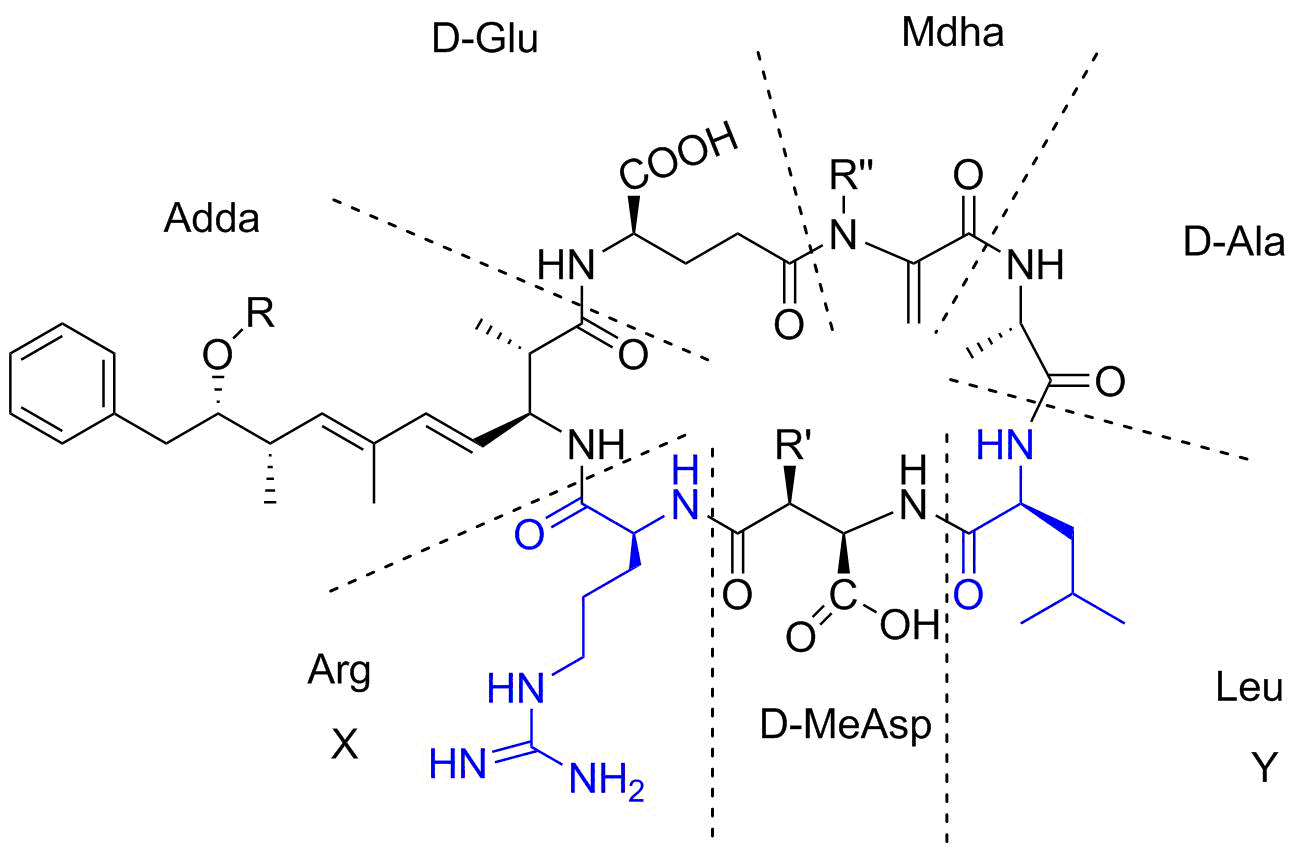
\includegraphics[width=\textwidth]{Microcystin-LR.eps}
  \caption{Structure of MC-LR}
  \begin{flushleft}
  a) Adda group responsible for the hepatoxicity
  b) L-leucine, a variable amino group amongst other congeners
  c) L-arginene, also a variable amino group in other congeners
  d) Methyl-group which can be demethylated in other congeners.
    \end{flushleft}
  \label{structure1}
\end{figure}





\section{Goals and Aims}

In our survey on 29 inland lakes in Michigan, we seek to build a predictive model on microcystins. In addition, we  measured for cylindrospermopsin and anatoxin-a to see if they are present in Michigan. Before the survey, I hypothesized if the lake's watershed is more urbanized areas I would expect higher microcystin concentrations. Developed land can increase nutrient rich runoff which can positive influence algal blooms. Previous studies shown developed areas having a major influence on the occurence of CHABs because of more possible sources like applied fertilizer or leaky septic tanks \cite{beaver_land_2014, anderson_harmful_2002}. Lakes with higher developed areas may also have a possible influence nutrient mobility, which in turn drive microcystin production.

One of our objective is to have a model that is simple and is robust in predicting HABs.
My goal is to explore what drives HABs and build a predictive model based from our collected data.  With the collected observations, I investigated the best possible predictive model from our dataset. Microcystin concentrations from LC-MS/MS and \emph{16S rRNA} gene copies will be tested as the response variable.
Some studies will assess cyanobacterial cell count or mass, concentrations of chloraphyll-a microcystin concentrations as a response variable as its most likely associated with HABs \cite{moore_richard_cyanobacterial_1993, ahn_evaluation_2011, jiang_statistical_2008, beaulieu_nutrients_2013, taranu_predicting_2017}. Cyanobacteria cell counts would be ideal for us to measure whether the lake is exhibiting a bloom. We currently are working on counting cells and unfortunately not completed thus far.  I used microcystin concentration as the main predictor variable of interest. I also observed the \emph{16s rRNA} gene copies as response variables as well as this measures relatively how much cyanobacteria there are based on the amount of 16S rRNA.

My research hypothesis:

\begin{enumerate}
\item Harmful algal blooms is influenced with land use attributes, specifically developed/urban land, which can be used to predict microcystin concentrations
\item Nutrient concentrations can be explained by land use characteristics
\item Identify important features from the collected dataset to build a predictve model for HABs.
\end{enumerate}


\chapter{SURVEY METHODS AND DESIGN}
\setlength{\parindent}{.5 in}
\raggedright\setlength{\parindent}{.5 in}



\section{Water Sampling} \label{sampling}

For the summer of 2017 a total of 29 inland lakes were sampled.  Prior to sampling, permission of riparian owner was obtained for most lakes which did not have public access. Sample surveying began on the month of June 2017 until October 2017. Each month every lake one was sampled once. Sampling locations were chosen from known list of lakes reported with HABs and existing collaborative partners. In addition, we also chose lakes that are reasonably close to I-75 expressway for the ease of transportation. See table \ref{table:Surveyed Lakes} for the list of sampled lake observed in our analysis and figure \ref{overview} for a map of our lake sites.

Water samples were collected by wading in toward the center of the lake until water height reached waist height. All water grab samples were taken roughly one foot below water surface.

Few of the lakes had public access areas for our sampling site. A total of 4 team of field surveyors sampled each with designated lakes. At each lake a hand-held multi-meter was used to measure pH, conductivity ($\mu$S/cm), dissolved oxygen (mg/L) and temperature ($^\circ$C). Phycocyanin and chlorophyll fluorescence were also measured using an Amiscience portable  with the optical excitation of 470nm and 590nm and the emission is read at 685nm, which is measured in relative fluorescence units (RFU). Each fluorometer for each lakey surveyor was calibrated against rhodamine WT dye as a secondary calibration standard, which ensure the data is relative to all other fluorometer. A portable HACH turbidity meter was used to measure turbidity in nephelometric turbidity unit (NTU). Formazin standards are used to calibrate the turbidity meter.



In July 2017 a constructed sampler float was installed at each lake. The sampler was constructed by the Dr. Raffel's team, which consisted with 3 plexi-glass plates and placed at each sampling location for the purpose of collecting zebra and quagga mussels (see figure \ref{samplerr}). The stack of three square plexiglass sheets are about 15,20, and 25cm in diameter which gives them a total surface area of 0.23 m$^2$ per sampler. Majority of sampler were installed on the riparian owner's dock or as a float. With the permission of riparian owners, the float is left in place for the  HOBO Pendant\texttrademark temperature and light logger were installed on floats at each lake site. Data was logged from July to October. In October, we collected the samplers and scraped all mussels into a glass mason jar for analysis of biomass. In addition, also installed a slotted PVC pipe which contains a Solid Phase Adsorbtion Toxin Tracking bag (SPATTS), a beta test of a new method of monitoring toxins. See appendix \ref{spattss} for more details.


Water sampling kits were prepared by storing pre-labeled water vessels stored in zip-lock bags for each lake. This was to prevent cross-contamination between different lake water samples during sampling transport and storage. Each sampling kit contained 60mL polyetheylene terephthalate (PETG) vials for microcystin analysis, 100mL sterile IDEXX\texttrademark bottles for QPCR analysis, 50mL polypropylene centrifuge vials and 250 mL HPDE Nalgene bottles for nutrient analysis. Each kit also provided alkaline lugols iodine solution for preserving cyanobacteria samples for identification and 6M \ch{H2SO4} for acid preservation of nutrient samples.



\begin{table}
\caption{List of surveyed Lakes with geographic location of sampling point}
\label{table:Surveyed Lakes}
\begin{center}
\scalebox{0.86}{
\begin{tabular}{|l|l|l|r|r|l|}
\multicolumn{1}{|c|}{Name of Lake} & \multicolumn{1}{c|}{Shorten Code} & \multicolumn{1}{c|}{County} & \multicolumn{1}{c|}{Longitude} & \multicolumn{1}{c|}{Latitude} & \multicolumn{1}{c|}{HUC 14 Reachcode} \\ \hline
Bear Lake & BEA & Kalkaska & -84.9438079727 & 44.7286139551 & 04060103001048 \\ \hline
Belleville Lake & BEL & Wayne & -83.4663770506 & 42.2145253455 & 04090005001822 \\ \hline
Bogie Lake & BOG & Oakland & -83.5054334514 & 42.6188513679 & 04090005001348 \\ \hline
Brighton Lake & BRI & Livingston & -83.7958137995 & 42.5169054061 & 04090005001500 \\ \hline
Coldwater Lake & COL & Isabella & -84.9565922285 & 43.6613607551 & 04080202000902 \\ \hline
Deer Lake & DEE & Charlevoix & -84.9770123186 & 45.166441811 & 04060105001116 \\ \hline
Ford Lake & FOR & Washtenaw & -83.5849122567 & 42.2159133043 & 04090005001823 \\ \hline
Houghton Lake & HOU & Roscommon & -84.7262816343 & 44.3385407778 & 04060102002461 \\ \hline
Hudson Lake & HUD & Lenawee & -84.2545514803 & 41.835000535 & 04100002001317 \\ \hline
Intermediate lake & INT & Antrim & -85.2293359783 & 45.0265435299 & 04060105003435 \\ \hline
Lake Cadillac & CAD & Wexford & -85.4266252378 & 44.2410192547 & 04060102001951 \\ \hline
Lake Margrethe & MAR & Crawford & -84.7830175986 & 44.6464747348 & 04060103001058 \\ \hline
Lake Nepessing & NEP & Lapeer & -83.3728265865 & 43.0161554865 & 04080204001601 \\ \hline
Lime Lake & LIM & Hillsdale & -84.3791188315 & 41.7861576065 & 04100006000872 \\ \hline
Little Glen Lake & LGL & Leelanac & -85.963633169 & 44.8687577197 & 04060104000456 \\ \hline
Little Round Lake & LRO & Lenawee & -84.3527742524 & 41.9093334799 & 04100006000858 \\ \hline
Manitou Lake & MAN & Shiawassee & -84.2038069227 & 42.925537136 & 04050005000939 \\ \hline
Ore Lake & ORE & Livingston & -83.7959940227 & 42.4805569493 & 04090005001574 \\ \hline
Paradise Lake & PAR & Emmett & -84.7512093045 & 45.6872890124 & 04060105001063 \\ \hline
Platte Lake & PLA & Benzie & -86.092789204 & 44.6900468421 & 04060104000558 \\ \hline
Pontiac Lake & PON & Oakland & -83.451096479 & 42.6664394508 & 04090005001288 \\ \hline
Posey lake & POS & Lenawee & -84.3007962072 & 41.8970465491 & 04100006000857 \\ \hline
Round Lake & ROU & Lenawee & -84.1318219224 & 42.0712488438 & 04100002001130 \\ \hline
Sanford Lake & SAN & Midland & -84.3860517762 & 43.7104273774 & 04080201001468 \\ \hline
Silver Lake & SIL & Grand Traverse & -85.687150728 & 44.6980286859 & 04060105003542 \\ \hline
Stony Creek Lake & STO & Oakland & -83.0870627175 & 42.7260717429 & 04090003001029 \\ \hline
Sugden Lake & SUG & Oakland & -83.4972563639 & 42.6173106359 & 04090005001347 \\ \hline
West Twin Lake & WTL & Montmorency & -84.3501403918 & 44.8762035424 & 04070007001271 \\ \hline
Wixom Lake & WIX & Gladwin & -84.3537506311 & 43.8276751177 & 04080201001442 \\ \hline
\end{tabular}}
\end{center}
\end{table}

\begin{figure}[!t]

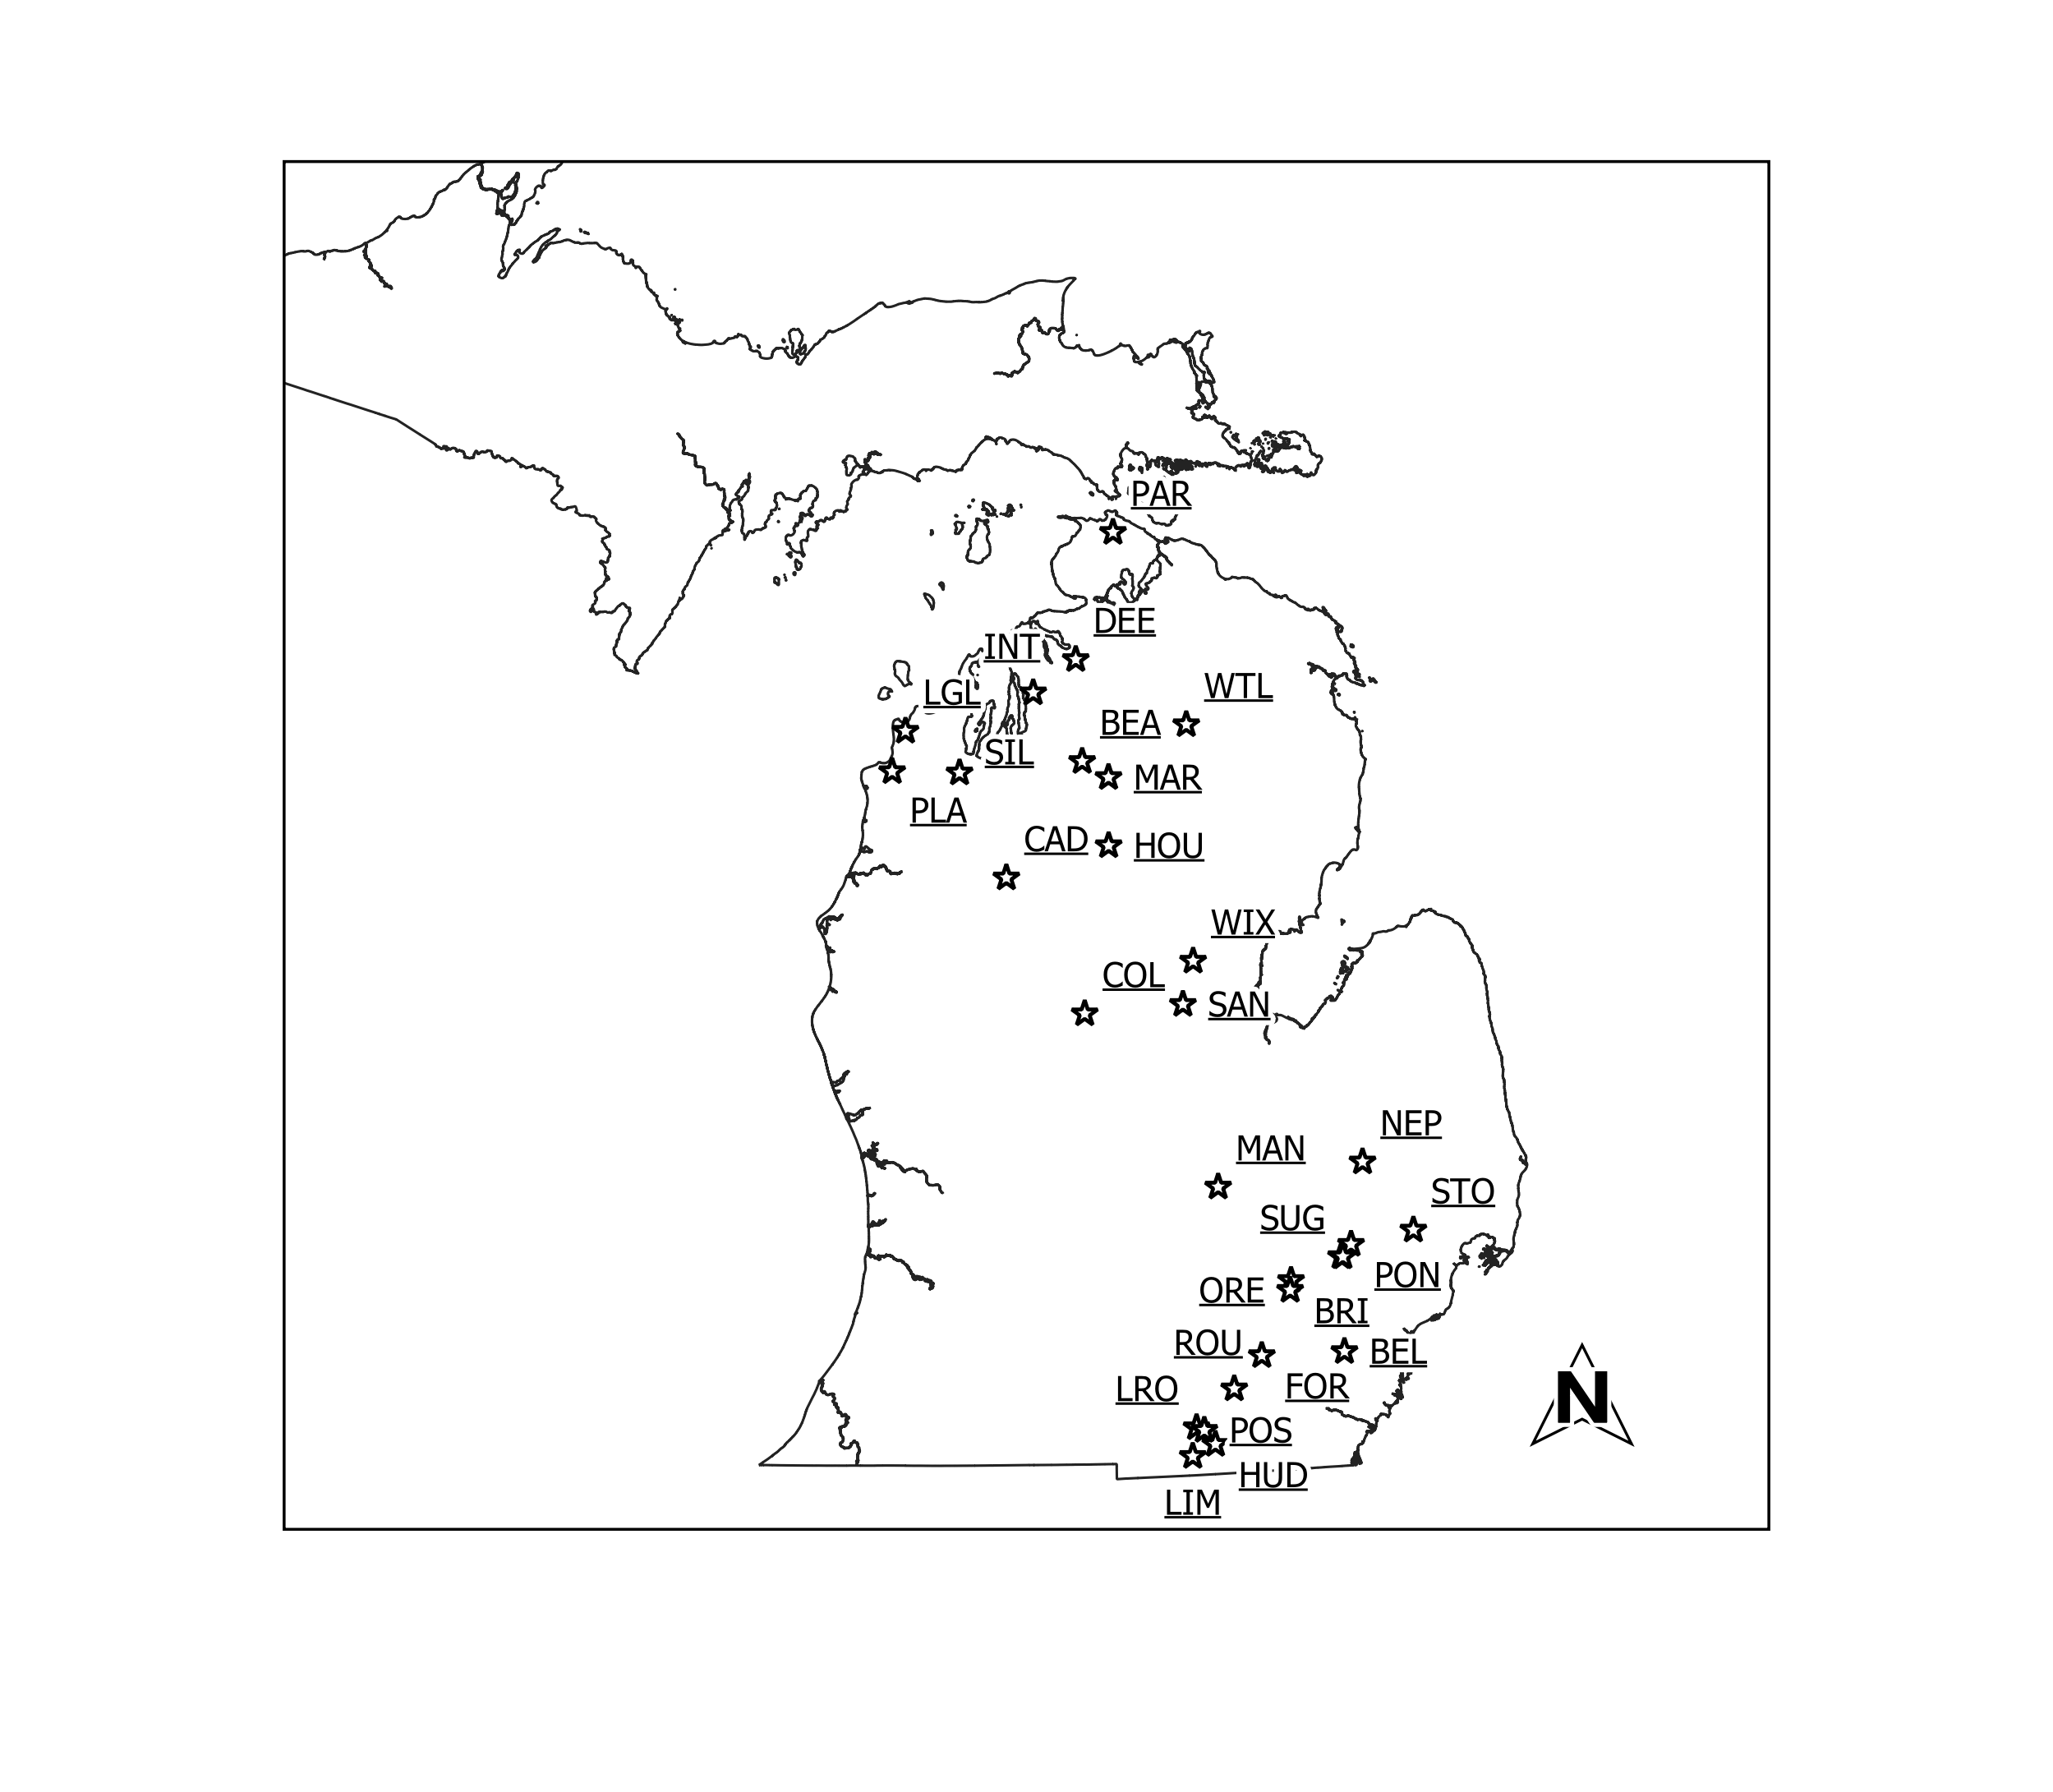
\includegraphics[width=\textwidth]{figures/Overview}
\label{overview}
\caption{Map of Sampled Lake Sites in Michigan}

\end{figure}

\begin{figure}[!ht]
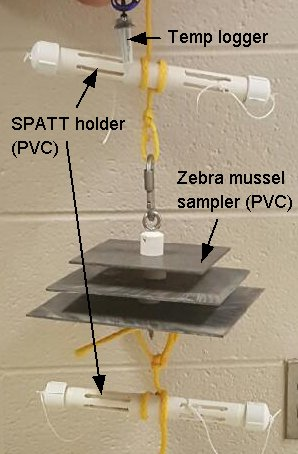
\includegraphics[width=\textwidth, angle =-90]{figures/samplers}
\caption{Picture of the constructed sampler installed at each lake}
\label{samplerr}
\end{figure}




\begin{figure}[!t]
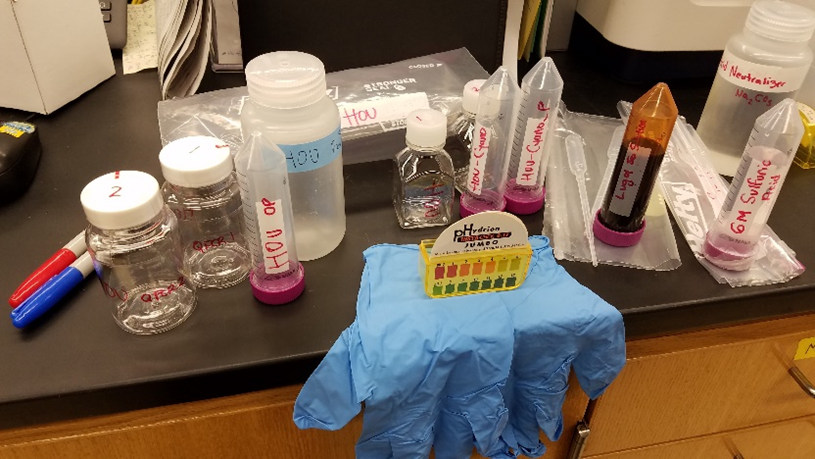
\includegraphics[width=\textwidth]{figures/samplekit}
\label{samplekit}
\end{figure}


\clearpage
\newpage

\section{Analysis}



\subsection{LC-MS/MS}

Water sample stored in 60mL PETG vials were freeze thawed for 3 cycles to lyse the cells.



A 3.5 ml aliquot of each sample above was transferred to glass vials suitable for the Thermo Scientific EQuan MAX (online sample concentrator).

Need to grab writeup from BRIAN was it filtered?????

These sample were transported to Wayne State University (WSU) and analyzed for 12 microcystin congeners, and nodularin.  The Westrick group at the WSU Lumigen Instrument Center (LIC) has developed a high-throughput LC-MS/MS analysis for microcystins in surface and drinking water analyses. The Westrick group’s LC-MS/MS platform includes a Thermo Scientific EQuan MAX (online sample concentrator) and ThermoFisher’s UltiMate 3000 (UHPLC) system and a TSQ Quantiva (MS/MS). The microcystin on-line concentration method is validated for 12 microcystins.

Their method is similar to EPA method 544 with the addition of 5 more congener analytes \cite{shoemaker_method_2015}. Figure \ref{spectra} shows a standard chromatogram of all 12 microcystins, nodularin, and the ethylated internal standard (C2D5 MC-LR) eluting between 2.2 – 5.2 minutes allowing for the total analyses time to be less than 12 minutes.  Minimum Detection limits (MDL) are 0.030  $\mu$g/L (or ppb) for microcystins.

\begin{figure}[h]
  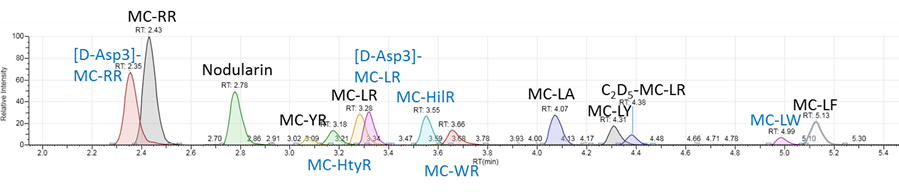
\includegraphics{LCMS_CONGENERS}
  \caption{Liquid chromotography-mass spectrometry chromatogram of the microcystin congeners}
  \label{spectra}
\end{figure}

\subsection{Nutrients}


Two 125-mL HPDE Nalgene bottles were used to collect acid-preserved water samples with 2mL of 3M \ch{H2SO4}, resulting to pH \textless 2. A 50 mL centrifuge tube is used to collect water sample without acid preservation for orthophosphate. One of the two nalgene bottle is allocated for ammonia-N and nitrate+nitrite-N by our lab at Oakland University and the other is for total phosphorus and total nitrogen run by Ben Southwell and his team at Lake Superior State University.  Samples were kept cool at 4 $^\circ$C during transport and stored at -20$^\circ$C. Upon receiving samples from field samplers samples are thawed if frozen and kept cool at 4$^\circ$C. All lake water samples are homogenized by inverting 8 times and aliquoted into 15-mL centrifuge vials and centrifuged at 3000rpm for 45 seconds. The supernatant was collected into a clean 3 mL vial and analyzed by AQ1 auto sampler. Ammonia-N is analyzed by an equivalent EPA method (USEPA Method 350.1), nitrate+nitrite-N analyzed by equivalent EPA method (USEPA Method 353.2), orthophosphate-P by equivalent EPA method (USEPA Method 365.1),total Kjeldahl nitrogen-N by equivalent EPA method (USEPA Method 351.2) and total phosphorus by equivalent EPA method (USEPA Method 365.1). All samples were analyzed within the appropriate time frame from time of sample.

\subsection{QPCR}

Phytoxigene CyanoDtec\texttrademark cyanobacteria and toxin test kit was preformed with Applied Biosystem StepOnePlus\texttrademark PCR. The kit provides two separate assay mix. Total cyanobacteria assay will quantify the 16srRNA gene copies found in the water sample. The toxin gene assay  were analyzed in parallel for each month of grab samples.  The PCR reaction mix contained 5 ul of template/sample extracts and 20 ul of rehydrated mastermix.  Each sample were run in singlicate due to limited amounts of reagent and budget. Positive standards for target genes  were run on each PCR analysis. CyanoNAS nucleic standards are removed from -20C and allowed to thaw prior to analysis.  Standards were run in duplicates.

Samples for QPCR were filtered either on site with portable Santino pump, or brought back to the lab for filtration within the day.
Each lake, 100mL or more of water sample was collected in a sterile IDEXX vessel then filtered through a 0.4$\mu$m pore size polycarbonate membrane  and stored at -20C until sampling route is back. Once filtered, they are immediately transferred into BioGX vials. BioGX vials are stored at -80C until analysis. BioGx vials contains 500 uL of lysis buffer, lysis beads and filtrate. For cell lysis, vials were vigorously shaken by bead beater for 2 minutes. After bead beaten, sample vials were centrifuged for 1 min. Supernatant was transferred to a microcentrifuge tube and centrifuged for 5 min, then transferred the final supernatant to another set of microcentrifuge tubes for PCR template.  Sample extracts are stored at 4C and analyzed within the day.



PCR heat cycles were programmed with initial denaturing step at 95$^\circ$C for 2 min, then a repeat of 95$^\circ$C for 15 seconds and 60$^\circ$C for 30 seconds reaching a total of 40 cycles. The appropriate gene targets filters were manually set to match the emission spectra of each probes. Each PCR run, standard curve is generated  from within the StepOnePlus software. CT threshold and baseline was manually assigned for each run by visually assessing each target run. The calculated gene copies are done automatically by the StepOnePlus software, expressed in gene copies/$\mu$L of lysate. The final reportable value is calculated by this equation:

\begin{center}
  $Genecopies/mL = (Genecopies/\mu L \: of \: lysate) \times (\frac{500\mu L \: of \: lysate}{\text{mL of Sample Volume}})$
\end{center}





\section{Watershed Characteristics}


Watershed delineation and calculation of land use was done using quantum geographic information system (QGIS) \cite{qgis_development_team_qgis_2009}.
Elevation data was downloaded in bulk by an FTP client as mosaic raster files for the state of Michigan downloaded from USGS (https://earthexplorer.usgs.gov/).
Elevation data  prepared by using $r.fill.dir$ function from GRASS which fills sinks or depressions \cite{grass_development_team_geographic_2017}. A flow accumulation raster map is generated from this command. The value of each cell designates the amount of flow based on drainage characteristics the elevation data. Visually viewing the histogram of the distribution of flow accumulation values, selecting the highest values displays will display the most probable areas the flow of water will be. This provided visual aid in selecting the pour point of each lake. A new shapefile was created and selected each lake's pour with the visual aid of stream flow lines. Using the $r.distance$ function from GRASS, i was able to snap each pour point to the proper place. Each lake's watershed was delineated using $r.drain$ to create a elevation model map derived from the flow accumulation raster file. The drainage raster file is then used as an input for function $r.water.outlet$ along with the coordinates of fixed pour point location, which gives the shape of each lake's watershed extent.

Land use data was downloaded from the 2006 National Land Cover Database \cite{development_completion_nodate}. The land use data were classified at anderson level-II, which has 20 different classification of land distinguishing different biomes and regions.  To simplify the land use data, the raster is reclassified into 8 anderson level-I categories using $r.recode$ tool from GRASS. The 8 anderson level-I classes are water, developed, barren, shrubs, forest, herbaceous and wetlands. Raster file was transformed into a vectorized shapefile. The shapefile was merged by union (or dissolved) by each lake's watershed, which resulted area of each land use class within each lake's watershed. This data was exported as a .csv file and prepared for statistical analysis.

Precipitation data were retrieved from the Global Historical Climatology Netowrk (GHCN) database from NOAA \cite{}. Daily precipitation data was downloaded from NOAA's FTP server (\url{ftp://ftp.ncdc.noaa.gov/pub/data/ghcn/daily/}).  The geolocation of each rain gauge station were imported into QGIS and mapped. The distribution of the rain gauges were not uniformally distributed. Thiessen/Voronoi polygons for each station were generated and overlayed on each watershed. The area of each thiessen/voronoi polygon's intersection with the corresponding catchmen is divided by the area of the lake's watershed to give a weighted value. The mean areal precipitation for each lake's watershed is calculated by taking each station's measurements and multiplying by the weighted value, then averaged together.  Ambient air temperature for each watershed is simply averaged together with their intersection of the lake's watershed. A multi-join was done in R using the \emph{dplyr} package for precipitation data with each sampled lake joined by lakes watershed \cite{wickham_dplyr:_2017}. Averaged 3, 5, 7, and 30 days lagged precipitation and ambient air temprature were calculated for our analysis.

\section{Statistical Modeling}

Each analytical measurement was compiled and organized by each sampling event. We have data sampled from Lake Superiour, Lake St. Clair and Lake Erie, however with my discussions with Dr. Szlag and Dr. Raffel, we decided to exclude them in our analysis.  Their unique geology and lake morphology does not fit our focus on inland lakes.
Data manipulation and analysis was done in Program R, a statistical computing language \cite{r_core_team_r:_2018}. The \emph{dplyr} package was used for data cleaning, compiling and preperation to have our dataset ready for statistical analysis \cite{wickham_dplyr:_2017}. Linear mixed models were used to analyze our data as this accounts for the variance of each of our lake site. The library package $lme4$ is used for our linear mixed modeling \cite{bates_fitting_2015}.

The requirements for building a linear model assumes the distribution of explanatory and response variables follow a normal distribution \cite{bates_fitting_2015}.
From our collected dataset, we assessed each variable's distribution and log-transformed to fit a normal distribution. To solve the problem of data values that are zero, we added the corresponding mininum detection limit first, then applied a log trasformation. See table \ref{variable} for a summary of which variable was transformed and the shorten variable name.

In our pursuit for finding important variables that potentially can explain our predictor variables, a best subsets regression analysis is used to find our features.  Measurements from each lake is a factor that may contribute as a random effect. This can be an issue where measurements from each lake is pseudoreplicated \cite{eisenhart_assumptions_1947}. Subset analysis is done on an averaged dataset based on each lake which works around this issue.
With the best variables from the regression subset, backward step-wise regression will be preformed to further refine the best fit model. Variables will be backwardly selected by F-test \cite{kenward_method_1987}. A linear mixed model will be used to verify our best models as it allows to account the variance of each sample site. Each non-nested models are rank by the lowest Bayesian Information Criterion (BIC) being our best model.


\chapter{RESULTS AND DISCUSSIONS}
\setlength{\parindent}{.5 in}
\raggedright\setlength{\parindent}{.5 in}


\section{Lake Results}

The compiled dataset with n=112 observations with some missing values.


Microcystin concentration displayed a slight curve when plotted against time peaking in the month of August. The average were low in June and October()

In our toxin analysis, we did not detect any cylindrospermonsin in our survey. We had one instance of anatoxin-a detected at Brighton lake in August 2017. From our QPCR analysis, we did not find any genes responsible for producing cylindrospermonsin (\emph{cyrA}), saxitoxin (\emph{sxtA}).  We found microcystin concentrations vary for each lake and through time. MC-RR, MC-LR and MC-LA were the most detected congeners in our survey. MC-RR was found with the highest concentrations 8.55 $\mu$g/L at Brighton Lake. We found varying amounts of \emph{mcyE} gene copies in each lake. Majority of our samples were below the EPA guidance level. From our sampled lake sites, Belleville, Brighton, Ford, Hudson, and Wixom Lake had instances of microcystin concentrations that exceeded the EPA guidance level of 4 $\mu$g/L (see figure \ref{microcystin}).

Mostly all of our sampled lakes were mostly alkaline conditions averaging around 8.53$\pm$0.37 pH ranging from 7.44 to 9.94. Dissolved oxygen averaged around 12.98$\pm$20.8 mg/L of \ch{O2}.

\section{\emph{A Priori} Hypothesis Test}

There were a slight positive trend with developed land-use plotted with log10(MC) concentration ,however the relationship is not significant  ($\beta=0.59$, $F_{{1,27}}=1.75$ , $p=0.20$). There was also no significant relationship between log10\emph{mcyE} gene copies and developed land use ($\beta=0.62$, $F_{{1,27}}=1.08$ , $p=0.30$), or with log10(\emph{16S rRNA}) gene copies ($\beta=0.48$, $F_{{1,25}}=1.75$ , $p=0.27$).
The amount  of zebra mussels did not significantly affect any of our response variables.
Forest land use had a significant negative relationship with \emph{16s rRNA} gene copies ($\beta=-1.42$, $F_{{1,25}}=7.08$, $p=0.013$). Albiet, forest land use did not have a significant effect on microcystin concentrations ($\beta=-0.34$, $F_{{1,26}}=0.32$, $p=0.57$).
The 16S rRNA gene copies has a signification positive relationship with microcystin concentrations.

Observing our correlation matrix (see \ref{matrix}), we can see some correlation between some of our variables. Land-use with nutrient concentrations. Agriculture had a positive effect on nitrate+nitrite,



\section{Feature Selection}

From our best subset analysis with the largest subset size of 4 (nvmax=4), we chose orthophosphate, total phosphate, turbidity,  and mcyE gene as our full model as its frequently chosen and persistent in each iteration (see figure \ref{subset}).

Total phosphate was not a signifigant predictor ($\beta=0.49$, $F_{{1,27}}=0.45$ $p=0.50$).
Microcystin concentration was signifigantly correlated with turbidity {$\beta=0.29$, $F_{{1,107}}=6.88$ $p=0.01$}

For predictive model for 16S rRNA gene copies, Chloraphyll, agriculture were chosen frequently in the subset analysis \ref{subset2}.

Total phosphorus did not show to have any signifigant relationship with any of our response variable.

\section{Discussions}






From , we wanted to deduce the idea of disturbance from developed land is associated with HABs. Disturbances of flora contributes to lower nutrient retention and hydrological impacts that can cause more blooms \cite{anderson_harmful_2002, codd_cyanobacterial_2000, fraterrigo_influence_2008}. From our data, we did not see a significant relationship between developed land use and any of our nutrient analysis.
Microcystin could increase as developed is more prevalent in the lake's watershed.

Other studies have found this relationship signifigantly positive.
One study on Lake Tai in China seeked to find correlation with fecal bacteria as a surrogate for urbanization and microcystin concentrations \cite{wilhelm_relationships_2011}.
They examined fecal bacteria asscociated with human population as a predictor. They did not find a signifigant correlation between human fecal bacteria and microcystin concentration or algal biomass \cite{wilhelm_relationships_2011}.
A statistical analysis study  on the EPA National Lake Assessment results found microcystin concentrations correlated to percentage of developed land use in the lakes watershed \cite{beaver_land_2014}. However in our data, we do not see a significant relationship. With each lake's watersheds characteristics,

A study in South Korea found 3-week lagged water temperature,dissolved oxygen and pH with to correlate with each other in their models \cite{ahn_evaluation_2011}.
We did not find

Growing cyanobacteria measurements taken at the same time . Their is an assumption being made.

Total nitrogen was found to explain the variance of microcystin concentrations \cite{taranu_predicting_2017}.

Man-made lakes are found to be twice as higher concentrations in cylindrospermonsin \cite{loftin_cyanotoxins_2016}.





Low-nutrient lakes can still exhibit blooms.
Cyanobacteria are versatile as they can acquire nutrients under extreme conditions. They can utilize a process called quorom sensing which they coordinate with each other by using a signaling hormone acylated homoserine lactones \cite{van_mooy_quorum_2012}. This creates a network of cells which work together as a unit, often as seen as a layer of green goo floating on top of water. This can complicate our model as this is not accounted for.

QPCR results as a response variable comes with complication as this does not distinguish alive or dead cyanobacteria.


Biological properties are not necessarily linear. One thing to consider here is the sampling frequency. We sampled once a month for four months, which gives four sampling results for each lake. This may not explain everything about each lake.

Failure to address ecological factors also can fail models. Previous studies in inland Michigan lakes are finding New Zealand Mudsnails to have an impact on finding blooms \cite{vanderploeg_zebra_2001}.


Water sampling for nutrient is difficult. Time series data, nutrient dynamic. Continuous measurements  water data would be best, but for a large survey its almost impractical. Other organisms compete with these common nutrients. Aquatic macrophytes largely acquire dissolved phosphorus. Nutrients acting as a stimulus could be a function similar to the shape of a Michaelis-Menton curve. Time between sampling the lake at the peak of the bloom and the flush of nutrient inputs can be lagged, and most likely different depending on each lakes morphology.

Bioavailability of phosphorus is pH dependent, where most is available between when in alkaline conditions greater \cite{lucas_relationships_1961}.




\begin{table}[!ht]
  \label{variable}
  \caption{List of coded measured variables and transformation}
\centering
\scalebox{0.66}{
\begin{tabular}{lll}
  \hline
Short Name & Variable Name (Units) & Transformation \\
  \hline
OP & Ortho-P (mg-P/L) & log10(OP + 0.003) \\
  NOX & Nitrate/Nitrite (mg-N/L) & log10(NOX + 0.04) \\
  NH3 & Ammonia (mg-N/L) & log10(NH3 + 0.006) \\
  TP & Total phosphorus (mg-P/L) & log10(TP + 0.002) \\
  TKN & Total kjeldahl nitrogen (mg-N/L) & log10(TKN + 0.07) \\
  TNTP & Total nitrogen to total phosphorus ratio & None \\
  X16SRNA & Cyano 16s rRNA gene copies (cp/mL) & log10(X16SRNA + 20) \\
  MCYE & mcyE gene copies (cp/mL) & log10(MCYE + 20) \\
  SUM & Microcysin sum from all 12 MC congeners (ppb) & log10(SUM + 0.03) \\
  wtemp & Water temprature at time of sampling (Celcius) & None \\
  pH & pH & None \\
  do & Dissolved oxygen (mg/L) & log10(do + 0.01) \\
  conduc & Conductance (uS/cm) & log10(conduc + 0.01) \\
  turb & Turbidity (NTU) & log10(turb + 0.01) \\
  chloro & Chloraphyll-a (RFU) & log10(chloro + 0.01) \\
  phyco & Phycocyanin (RFU) & log10(phyco + 0.01) \\
  TN & Total nitrogen (mg-N/L) & log10(TN + 0.116) \\
  Max\_Depth & Maximum depth of lake (meters) & None \\
  Lake\_Area\_sqKm & Lake area (sq Km) & log10(Lake\_Area\_sqKm + 1) \\
  Watershed\_Area\_sqKm & Watershed Area (sq Km) & log10(Watershed\_Area\_sqKm + 1) \\
  Lake Area\_Watershed Ratio & Lake area to watershed area ratio & log10(Lake Area\_Watershed Ratio + 1) \\
  Water & Land-Use percentage in lakes watershed & None \\
  Developed & Land-Use percentage in lakess watershed & None \\
  Barren & Land-Use percentage in lakes watershed & None \\
  Forest & Land-Use percentage in lakes watershed & None \\
  Shrubs & Land-Use percentage in lakes watershed & None \\
  Herbaceous & Land-Use percentage in lakes watershed & None \\
  Agriculture & Land-Use percentage in lakes watershed & None \\
  Wetlands & Land-Use percentage in lakes watershed & None \\
  LogMusselMass & Zebra mussel Mass (grams) & log10(MusselMass + 1) \\
  LogMusselNum & Zebra mussel counts & log10(MusselNum + 1) \\
  precip3 & Average precipitation 3 days before sampling  (mm) & log10(precip3 + 1) \\
  temp3ambient & Average temperature 3 days before sampling (Celcius) & None \\
  precip5 & Average precipitation 5 days before sampling (mm) & log10(precip5 + 1) \\
  temp5ambient & Average temperature 5 days before sampling (Celcius) & None \\
  precip7 & Average precipitation 7 days before sampling (mm) & log10(precip7 + 1) \\
  temp7ambient & Average temperature 7 days before sampling (Celcius) & None \\
  precip30 & Average precipitation 30 days before sampling (mm) & log10(precip30 + 1) \\
  temp30ambinet & Average temperature 30 days before sampling(Celcius) & None \\
  hobotemp & Average Temprature from Hobo pendant one month before sampling (Celcius) & None \\
  hobolight & Average light intensity from Hobo pendant one month before sampling (lux) & log10(hobolight +1) \\
   \hline
\end{tabular}}
\end{table}

\begin{figure}[!ht]
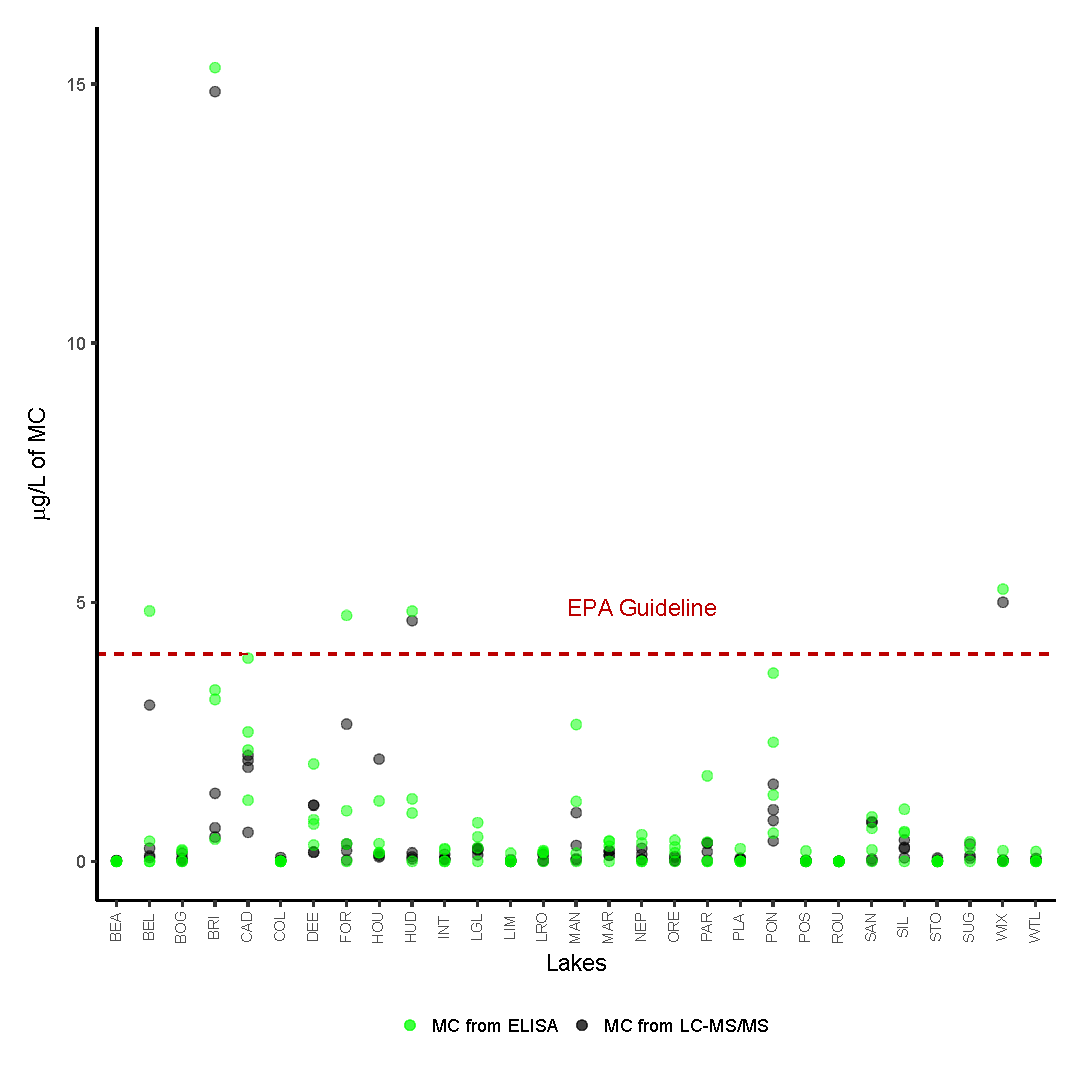
\includegraphics[scale=0.8]{figures/Microcystin}
\caption{Total microcystins by each lake}
\label{microcystin}
Microcystin results from ELISA and LC-MS/MS are plotted by each lake.
\end{figure}

\begin{figure}[!ht]
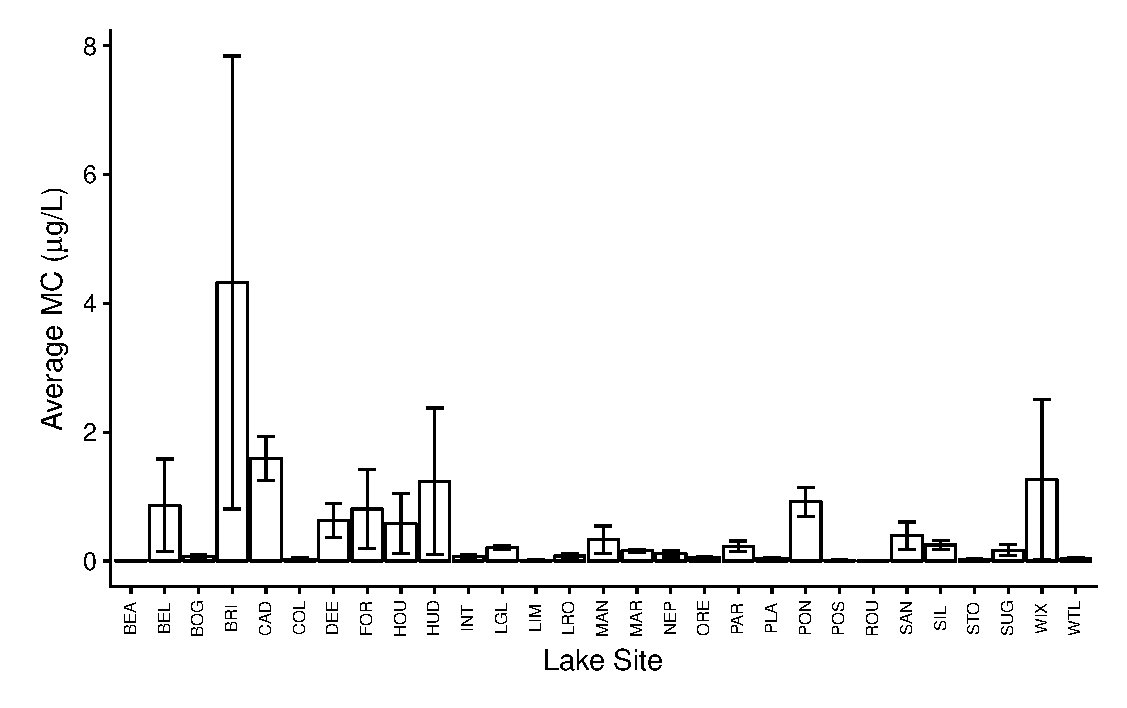
\includegraphics{figures/barmcsum}
\caption{Average total microcystin of each lake measured by LC-MS/MS}
\label{mcbar}
\end{figure}



\begin{figure}[!ht]
  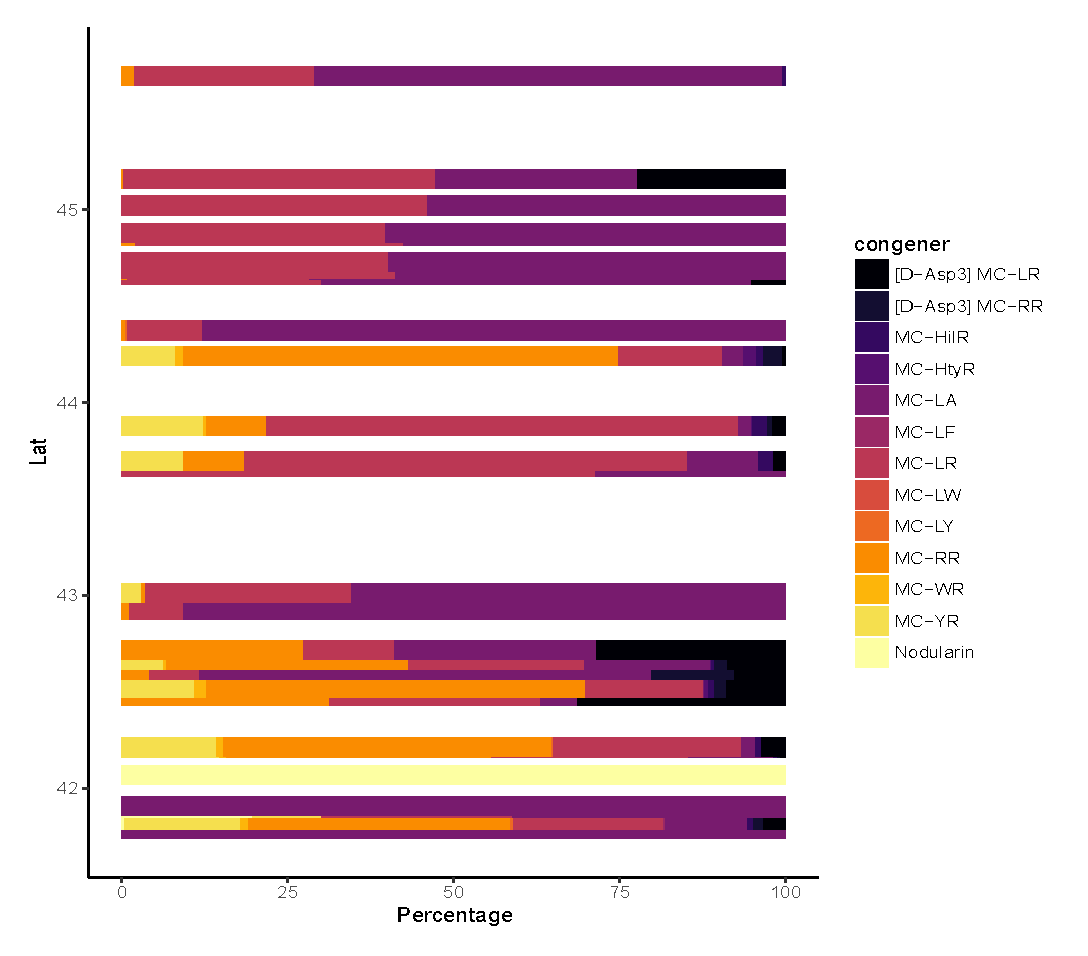
\includegraphics[scale=0.9]{congeners}
    \caption{Proportion of MC congeners plotted by latitude}
  \label{congenerlat}
\end{figure}

\begin{figure}[!ht]
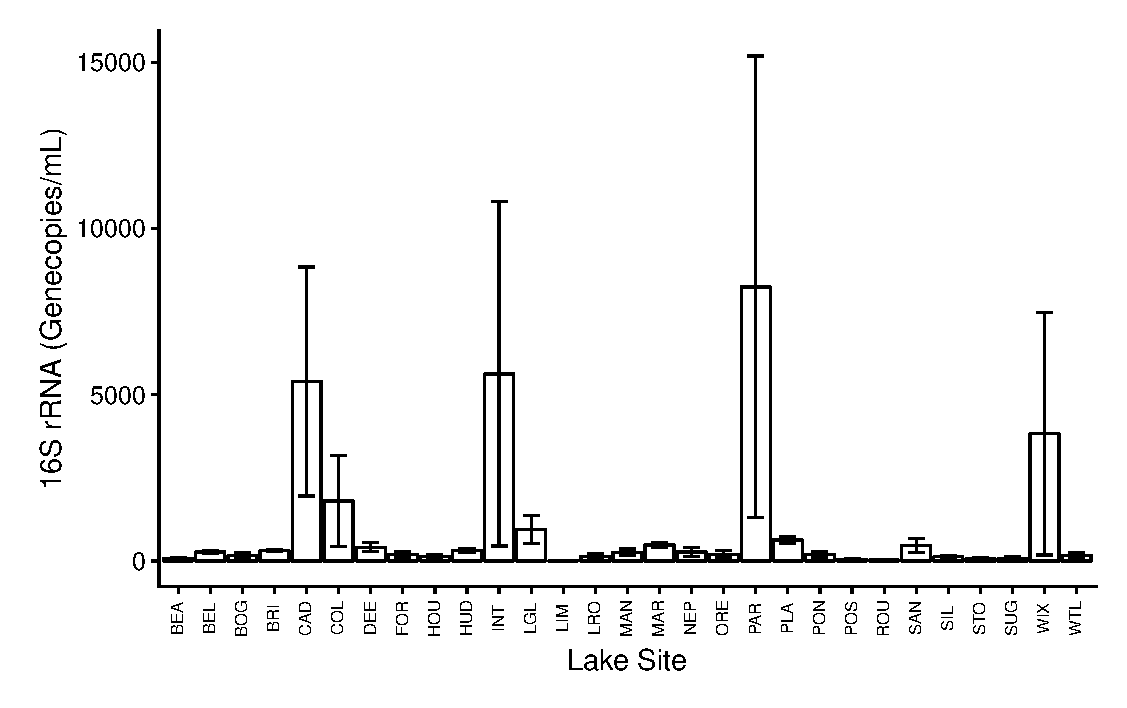
\includegraphics{figures/bar16srna}
\caption{Average 16S rRNA Genecopies/mL of sample by each lake}
\label{box16srna}
\end{figure}

\begin{table}[!ht]
\centering
  \caption{Microcystin congener statistical summary}
  \label{}
\begin{tabular}{@{\extracolsep{5pt}}lccccc}
\\[-1.8ex]\hline
\hline \\[-1.8ex]
Statistic & \multicolumn{1}{c}{N} & \multicolumn{1}{c}{Mean} & \multicolumn{1}{c}{St. Dev.} & \multicolumn{1}{c}{Min} & \multicolumn{1}{c}{Max} \\
\hline \\[-1.8ex]
Nodularin & 114 & 0.0003 & 0.002 & ND & 0.021 \\
{[D-Asp3]}MC-RR & 114 & 0.006 & 0.028 & ND & 0.255 \\
MC-RR & 114 & 0.185 & 0.855 & ND & 8.552 \\
MC-YR & 114 & 0.046 & 0.202 & ND & 1.799 \\
MC-HtyR & 114 & 0.002 & 0.012 & ND & 0.107 \\
MC-LR & 114 & 0.142 & 0.447 & ND & 3.570 \\
{[D-Asp3]}MC-LR & 114 & 0.027 & 0.107 & ND & 0.902 \\
MC-HilR & 114 & 0.004 & 0.019 & ND & 0.150 \\
MC-WR & 114 & 0.005 & 0.029 & ND & 0.302 \\
MC-LA & 114 & 0.088 & 0.196 & ND & 1.729 \\
MC-LY & 114 & 0.0004 & 0.002 & ND & 0.024 \\
MC-LW & 114 & ND & ND & ND & ND \\
MC-LF & 114 & 0.0002 & 0.001 & ND & 0.012 \\
MC Sum from LC MS/MS  & 114 & 0.505 & 1.580 & ND & 14.857 \\
MC from ELISA & 115 & 0.747 & 1.784 & ND & 15.320 \\
\hline \\[-1.8ex]
\multicolumn{6}{r}{Values are expressed as($\mu$g of MC*${L^{-1}}$)} \\
\end{tabular}
\end{table}



\begin{table}[!ht]
  \centering
  \caption{QPCR statistical summary table}
  \label{QPCR}
  \begin{tabular}{@{\extracolsep{5pt}}lccccc}
  \\[-1.8ex]\hline
  \hline \\[-1.8ex]
  Statistic & \multicolumn{1}{c}{N} & \multicolumn{1}{c}{Mean} & \multicolumn{1}{c}{St. Dev.} & \multicolumn{1}{c}{Min} & \multicolumn{1}{c}{Max} \\
  \hline \\[-1.8ex]
  16S rRNA & 112 & 405,761 & 798,946 & ND & 6,765,631 \\
  mcyE & 91 & 8,517 & 49,396 & ND & 467,174 \\
  cyrA & 93 & ND & ND & ND & ND \\
  sxtA & 93 & ND & ND & ND & ND \\
  \hline \\[-1.8ex]
  \multicolumn{6}{r}{* Values are expressed as Gene copies/$\mu$L} \\
  \multicolumn{6}{r}{ND=No Detects} \\
  \end{tabular}
  \end{table}



  \begin{figure}[!ht]
  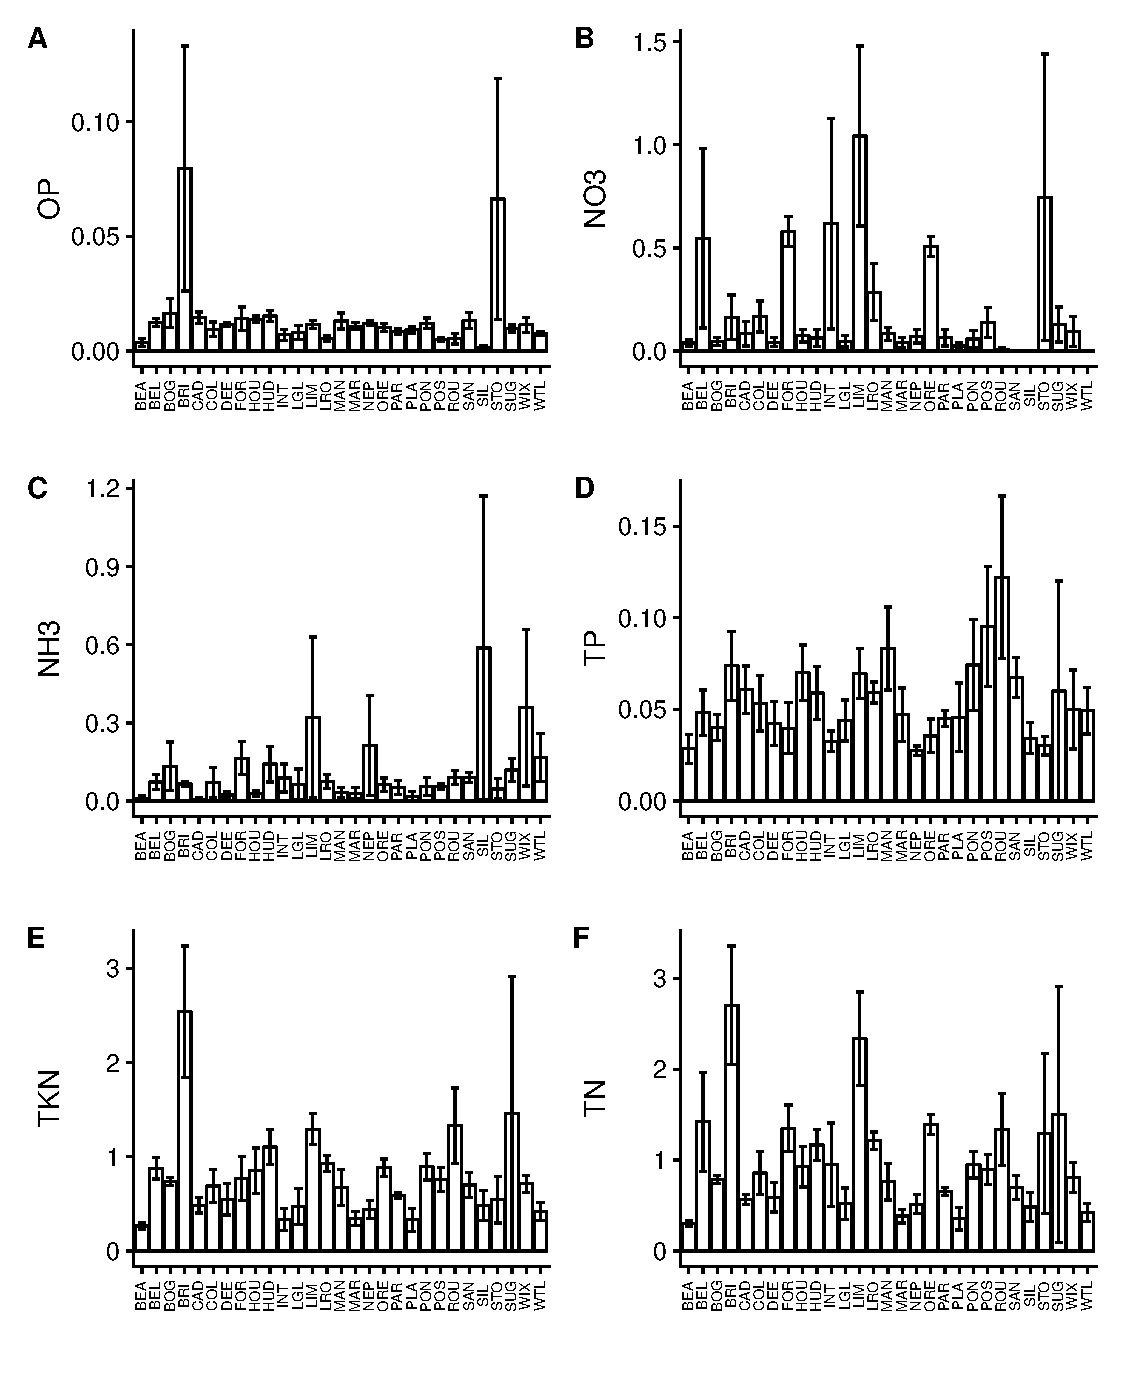
\includegraphics[width=\textwidth, height=15cm]{figures/nutboxplotlake}
  \caption{Nutrients}
  \end{figure}




  \begin{table}[!ht]
    \centering
    \caption{Lake nutrients statistical summary}
    \label{}
  \begin{tabular}{@{\extracolsep{5pt}}lccccc}
  \\[-1.8ex]\hline
  \hline \\[-1.8ex]
  Statistic & \multicolumn{1}{c}{N} & \multicolumn{1}{c}{Mean} & \multicolumn{1}{c}{St. Dev.} & \multicolumn{1}{c}{Min} & \multicolumn{1}{c}{Max} \\
  \hline \\[-1.8ex]
   Orthophosphate (mg P/L) & 114 & 0.015 & 0.030 & 0.000 & 0.237 \\
  Nitrate+Nitrite (mg N/L) & 115 & 0.199 & 0.443 & 0.000 & 2.827 \\
  Ammonia (mg N/L)  & 115 & 0.112 & 0.281 & 0.000 & 2.338 \\
  Total Phosphorus (mg P/L) & 114 & 0.055 & 0.037 & 0.000 & 0.239 \\
  Total Kjeldahl Nitrogen (mg N/L) & 114 & 0.763 & 0.602 & 0.000 & 4.555 \\
  Total Nitrogen & 114 & 1.074 & 0.870 & 0.103 & 4.717 \\
  \hline \\[-1.8ex]
  \end{tabular}
  \end{table}





\begin{figure}[!ht]
  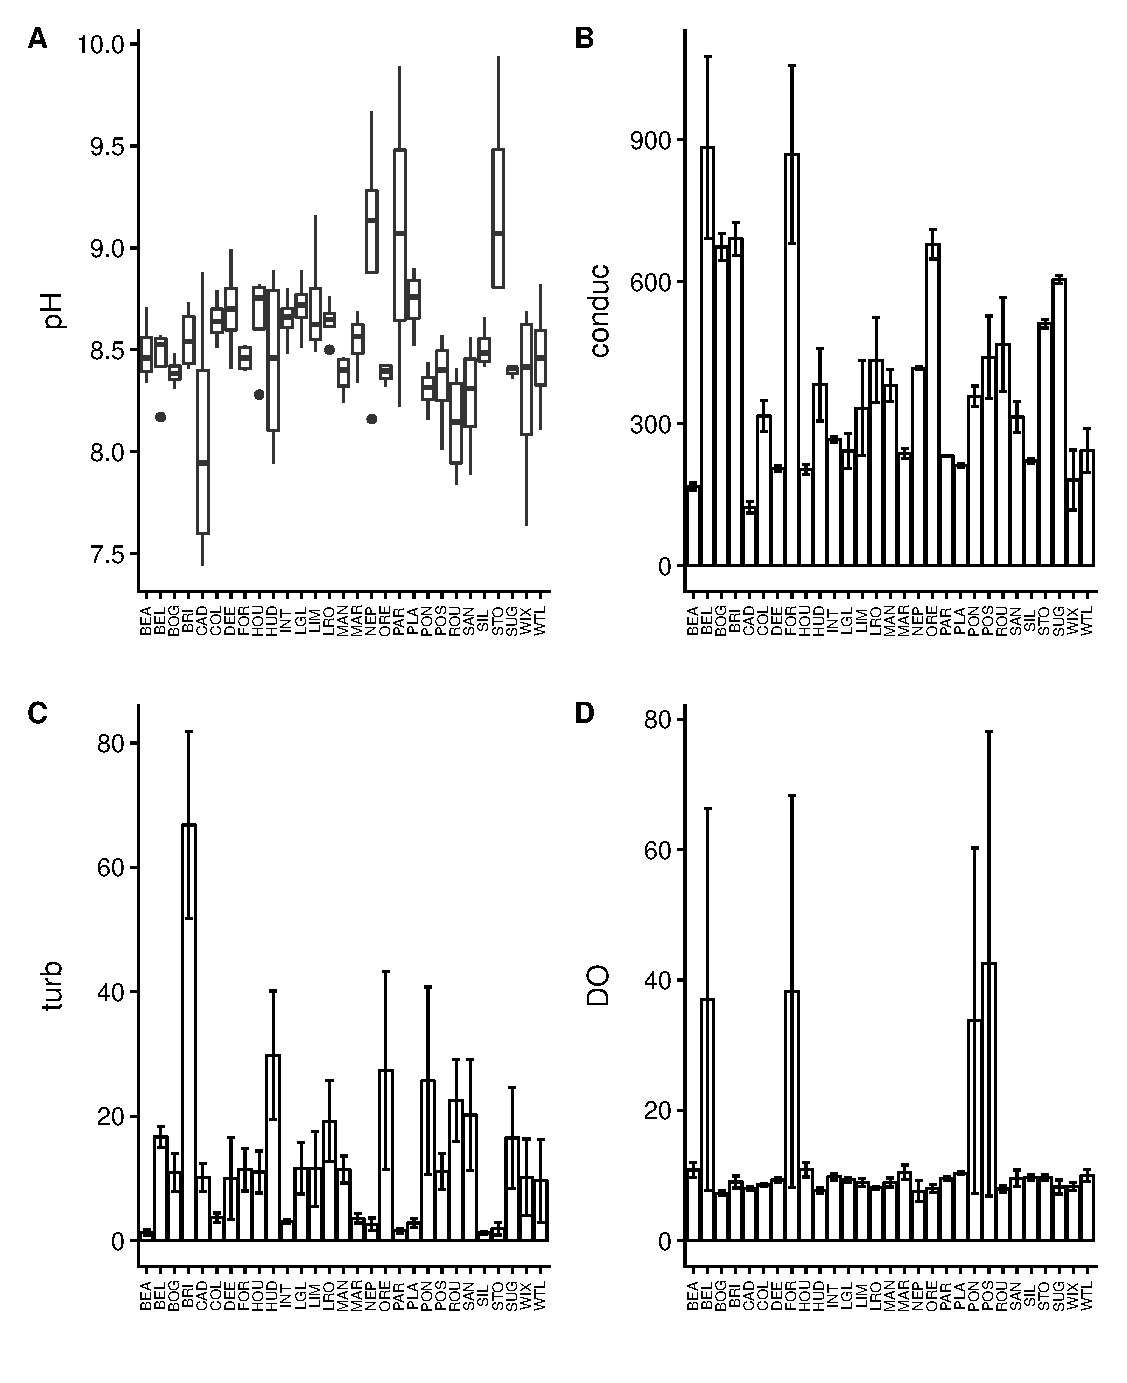
\includegraphics{figures/watboxplotlake.eps}
  \caption{Water chemical parameters}
  (A) Boxplot of pH for all (A).
\end{figure}



\clearpage
\newpage


\begin{figure}[!ht]
  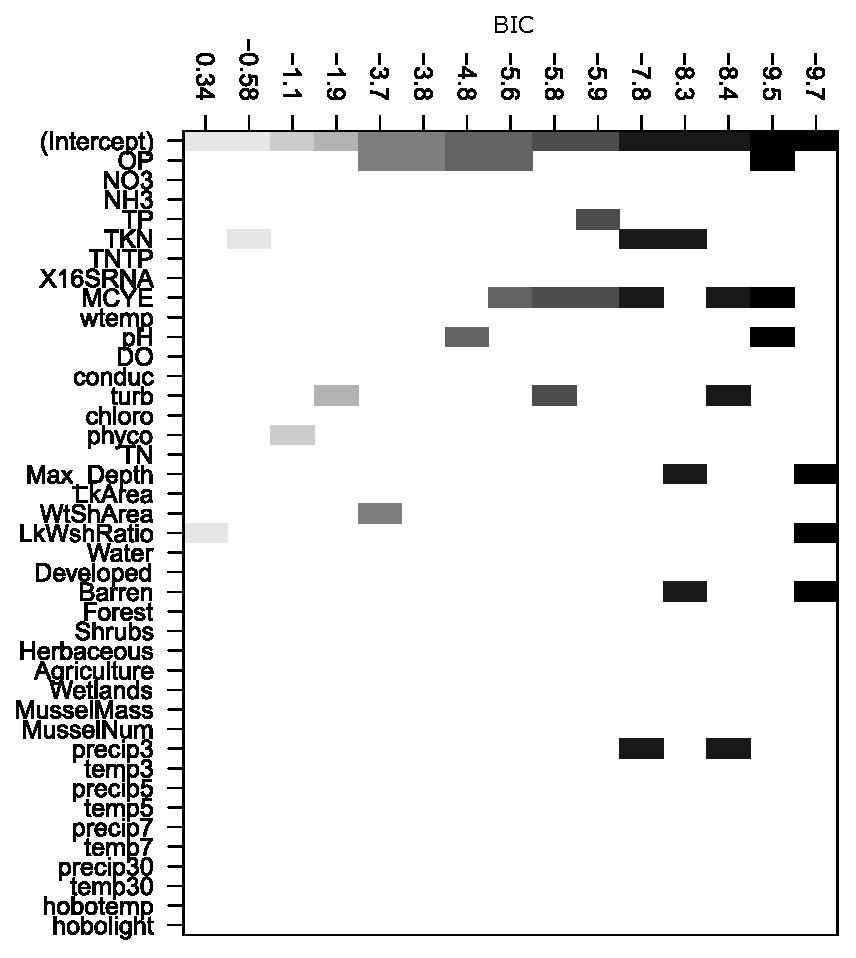
\includegraphics[width=\textwidth]{Subset}
  \caption{Best Subset: MC Sum from LC-MS/MS as response variable}
  \label{subset}
  Each row is a model, if a variable is included in the model it is represented as a shaded rectangle. The BIC is plotted on the y axis where the lowest value is higher up on the axis. The better the model, the lower the BIC, thus the top rows are the better model.
\end{figure}

\begin{figure}[!ht]
  \caption{Correlation Matrix}
  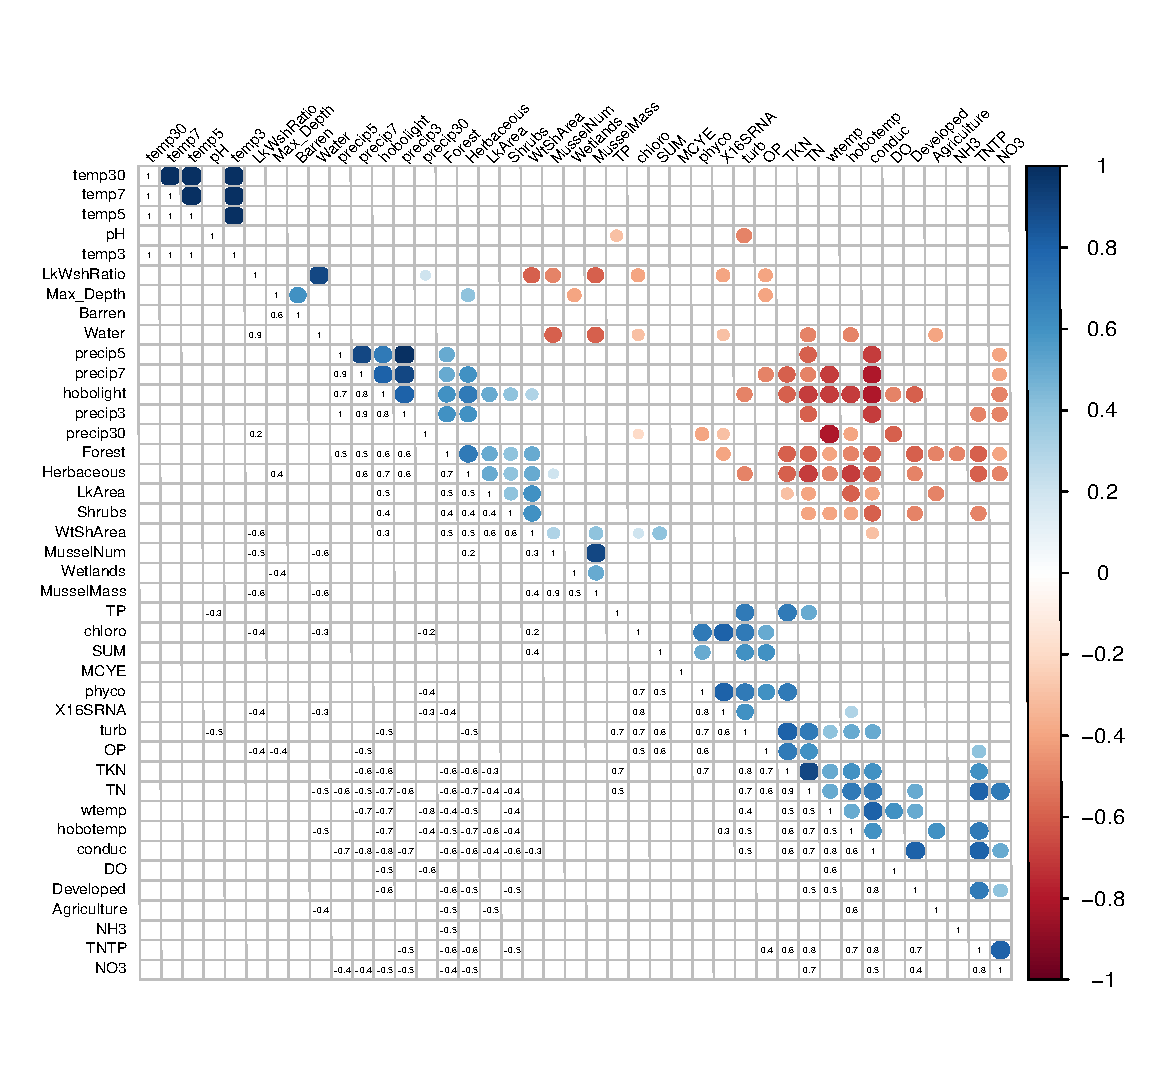
\includegraphics{matrix}
  Positive correlation is represented with solid blue box and negative correlation with scored box.
  \label{matrix}
\end{figure}



\begin{figure}[!ht]
  \includegraphics{Subset2}
  \caption{Best Subset: \emph{16s rRNA} Gene copies as response variable}
  \label{subset2}
\end{figure}


\chapter{CONCLUSION}
\setlength{\parindent}{.5 in}
\raggedright\setlength{\parindent}{.5 in}




Using a predictive model can potentially be a vital utility for protecting the public from HABs. Protecting public health is a balance of scientific knowledge, risk assessment of the situation and maximizing available tools at our disposal. It is apparent that it is difficult to model such a complex dynamic. In general there are no best models in an ideal sense, but statistical modeling can help identify meaningful relationships. Point sampling does not encapsulate all the complex relationship and does not explain subtle changes. Confounding variables such as unaccounted disturbances not measured from our survey is not accounted. 

We are currently exploring artificial neural-networking to model our full dataset.


\clearpage
\newpage

\bibliographystyle{biochem.bst}
\bibliography{sources}
\begin{appendix}
\appendixchapter{Solid Phase Adsorption Toxin Tracking} \label{spattss}


\section*{SPATTs}
Solid Phase Adsorption Toxin Tracking (SPATTs) is new unique method of monitoring waterbodies. A Nitex mesh bag containing HP-20 resin (styrene-divinylbenzene copolymer) is submerged in waterbody of interest for a period of time. During this period, free-floating compounds will adsorb onto the polymer beads. SPATTs can are then retrieved and analyzed for chemical analytes of interest. This technique can be useful if sampling frequency is financially limited..





\section*{Methods}

A 1 meter x 5 centimeter strip of Nitex mesh were precisionaly cut. The Nitex strip was sewn by folding half lenth-wise (or \emph{hot dog} style). With tape holding the fold, the end of the strip was sewn 0.5cm from the edge. Stiching design was tight to ensure no leakage of polymer beads.

9-10cm of sewn Nitex strips were cut and zip-tied about 0.5cm at one end. 3.00-3.01 grams of HP-20 resin was filled using a funnel. The other end is zip-tied once the Nitex bag is full. SPATT bags are activated by soaking in 100\% methanol for 24 hours under $4^\circ$C. Next the SPATTs were rinsed with Milli-Q water and then soaked for 24 hours in Milli-Q water under $4^\circ$C before deploying the SPATTs bag in our target sample lakes.

At each lake site, two SPATT bags were loaded into a slotted PVC pipe. At each lake, a float was installed as described in section \ref{sampling}. SPATTs are left for about a month at each lake. When SPATTs are retrieved, they are carefully removed and rinsed with Milli-Q water and stored in a 15mL centrifuge vial with a plastic spacer on the bottom. SPATTs are stored at $4^\circ$ during transport back to the lab. The SPATTs are centrifuged at 8000rpm. The spacer allows liquid to pool on the bottom when centrifuged. When centrifuged, the SPATT bags are cut open and the resin is poured into a 50mL centrifuge tube. Milli-Q water is used to rinse the SPATT bags to effectivly transfer all the resin. About 30mL of Milli-Q water is used. The solution is allowed to rest so the resin settles to the bottom. Using a pipet, the water is carefully decanted until the total volume is 5mL.  A solution of 80\% methanol with 10$\mu$M ammonium formate is added to the tube until the total volume is 50mL. The solution is gently mixed and then allowed to settle for 30 minutes.

\section*{Results}

Out of all 12 congeners, MC-LA, MC-LR, and MC-RR were the most frequently detected congener.

\begin{table}[!ht]
\centering
  \caption*{Microcystin Congener from SPATTs}
  \label{}
\begin{tabular}{@{\extracolsep{5pt}}lccccc}
\\[-1.8ex]\hline
\hline \\[-1.8ex]
Statistic & \multicolumn{1}{c}{N} & \multicolumn{1}{c}{Mean} & \multicolumn{1}{c}{St. Dev.} & \multicolumn{1}{c}{Min} & \multicolumn{1}{c}{Max} \\
\hline \\[-1.8ex]
{[D-Asp3]}MC-RR & 91 & ND & ND & ND & ND \\
MC-RR & 91 & 164 & 1,116 & ND & 10,380 \\
Nodularin & 91 & 2 & 17 & ND & 160 \\
MC-YR & 91 & 10 & 30 & ND & 145 \\
MC-HtyR & 91 & 0 & 2 & ND & 18 \\
MC-LR & 91 & 353 & 1,211 & ND & 8,146 \\
{[D-Asp3]}MC-LR & 91 & 2 & 10 & ND & 92 \\
MC-HilR & 91 & 1 & 6 & ND & 53 \\
MC-WR & 91 & 0 & 1 & ND & 7 \\
MC-LA & 91 & 534 & 2,063 & ND & 13,977 \\
MC-LY & 91 & 1 & 11 & ND & 101 \\
MC-LW & 91 & 0 & 0 & ND & 0 \\
MC-LF & 91 & 0 & 2 & ND & 18 \\
Total MC & 91 & 1,066 & 3,273 & ND & 22,124 \\
\hline \\[-1.8ex]
\multicolumn{6}{r}{Values are expressed as (ng of MC / gram of resin)} \\
\end{tabular}
\end{table}

\begin{figure}[!ht]
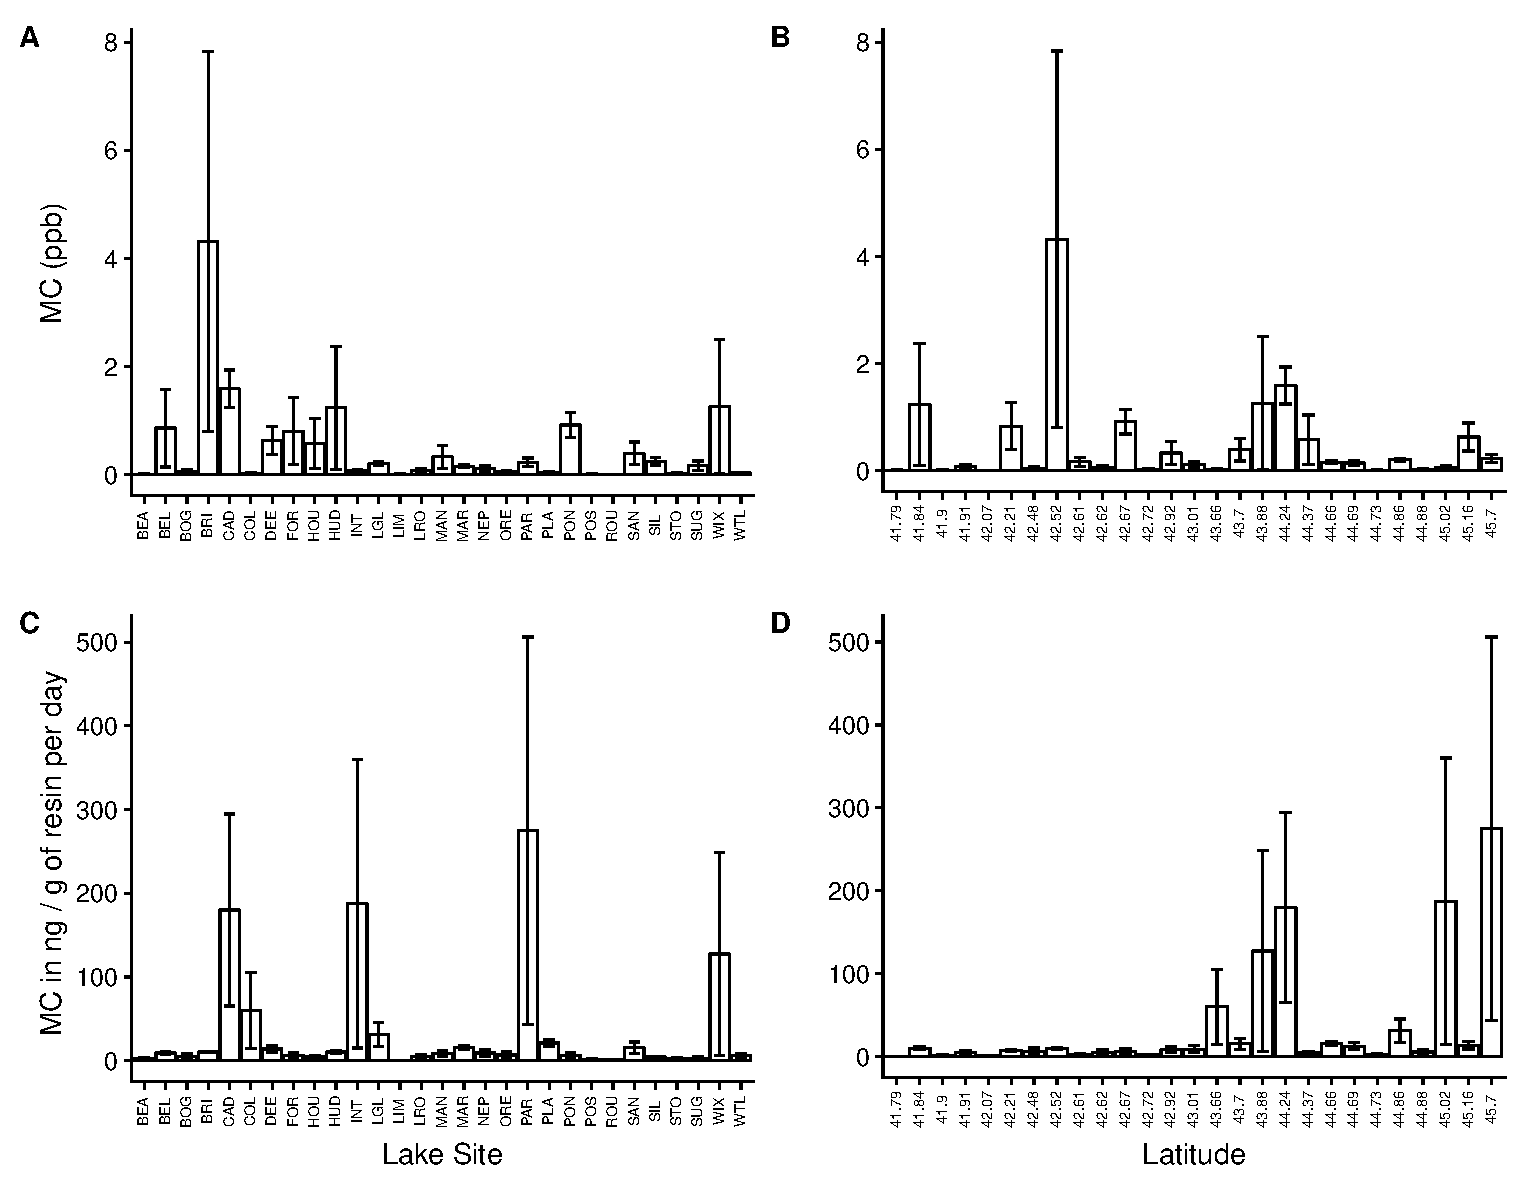
\includegraphics[width=\textwidth]{figures/spatttboxplotlake}
\label{spattbox}
\caption*{Comparitive Results of Microcystin Measured from SPATTS and Grab Samples}
A) B) C) D)
\end{figure}


\clearpage
\newpage


\appendixchapter{Data Collection Using Open Data Kit}

\GrizzAppendix{Geospatial Data Collection Guide Using Open Data Kit}

\GrizzAppendixSection{Introduction}

Collaborative work is the fundamental part of a large scale research project.  Data aggregation and structural collection is one of the few key factors that determines the quality of the study. Large scale studies are often done by a team of multiple groups and organizations. There are available commercial tools which can aid in data collection and aggregation automatically. ArcGIS \footnote{ESRI 2017. ArcGIS Desktop: Release 10.5.1 Redlands, CA: Environmental Systems Research Institute.} coupled with their Android/IOS app called Collector for ArcGIS \footnote{https://www.esri.com/products/collector-for-arcgis}.

From my experience I found a viable alternative which does not require an expensive license. I wish to help other research studies with a cheaper alternative and greatly facilitate their pursuit. I have written this guide to allow anyone to build from the ground up on setting a database and providing a viable way to organize an enterprise. This guide is aimed to initially setup a database for non-profit organization and academic research with a limited budget. The initial cost is \$5 per month for a virtual private server (VPS) which has enough storage for a small database.  The software tool is from an open-source software by \gls{odk}\footnote{Open Data Kit 2.0: Expanding and Refining Information Services for Developing Regions \url{http://www.hotmobile.org/2013/papers/full/2.pdf} Waylon Brunette, Mitchell Sundt, Nicola Dell, Rohit Chaudhri, Nathan Breit, Gaetano Borriello In HotMobile, 2013. \url{http://dl.acm.org/citation.cfm?id=2444790}}.

\GrizzAppendixSection{Required Components}

Here you must setup a server that stores you data and be accessible through the Internet. Having your own computer machine as a server is a viable solution but it requires more extensive networking knowledge. An alternative solution is to purchase a rent a server from a third party which automatically sets up and quickly gets connected to the Internet. A Virtual Private Server (VPS) are cheap and flexible servers to set up a database up on the cloud. For as little as \$5 dollars a month one can have a server with everything they need to start collecting data.

DigitalOcean, Amazon (free trial for a year), Google VPS can work. I suggest anyone of them, but in this guide we will choose to setup from DigitalOcean as its the cheapest available server. I recommend Debian or Ubuntu linux distribution to setup your database. In this guide, we will choose Debian 9 (Stretch).

\GrizzAppendixSection{Syntax}
\noindent
In the terminal, you will need bash commands to setup the server's configuration. In this guide, bash commands will be represented the \$ symbol. Each line of code is represented with a single \$ at the beginning. Enter the text following anything after the \$. With some lines of code, there will be included comments which will be represented by the \#.

\begin{lstlisting}
  $ run this command   # This is a comment
\end{lstlisting}

\noindent
Note that the first line starts with a\#. This is not a command but a comment. In bash language, this is usually ignored. In this guide, a line starting with \$ designates a command. Do not include the \$ as its merely a symbol to designate a command. Running lines will not have \$ as its indented to be one line of code.

\GrizzAppendixSection{Server Setup}

\noindent
You must get an SSH client to access the server for setting up ODK Aggregate. For Linux or Mac, use the native terminal application to access the server. For windows users, I recommended program is PuTTy \url{https://www.putty.org/}. Install this program for windows. With PuTTy, open up PuTTy and enter in the IP address and click ``Open''. You will enter ``root'' and the password given by the online service or by the user installation setup.  Usually when using VPS services, the IP address and the password for user \emph{root} information is given by email.
\noindent
The command for linux or mac users, they can use Terminal and use this command:
\begin{lstlisting}[language=bash]
  $  ssh root@[EnterYourIp]   # SSH with root as user
  #  replace [EnterYourIp] with the given IP address
\end{lstlisting}

\noindent
From a fresh installation, the first prompt when accessing the server will be to change your password. Choose a good strong password for the root username and have it written down.  After setting the password, preform any upgrades and install sudo which allows a normal user to have elevated privileges and install nano, a text editor. This may be already installed but some distributions might not have them. To do this, follow these commands.

\begin{lstlisting}[language=bash]
  $  apt update            # Use the apt package manager and update repository
  $  apt upgrade -y        # Preform any upgrades
  $  apt dist-upgrade -y   # Distribution upgrades
  $  apt install sudo nano # Install the sudo and nano packages
\end{lstlisting}

\noindent
Next, we will set a separate username. The \emph{root} user is only used to administer the server.  Choose any name as you see fit and something you can remember. For our example, for the case of this guide, \emph{dummy} will be the username.

\begin{lstlisting}[language=bash]
  $  adduser dummy
\end{lstlisting}

\noindent
You will be prompted to create a password. When asked for name and other user information, hit ``Enter'' to leave it blank. This does not need to be filled out.

\noindent Here, we will also assign this new user as a sudo user. This will enable the new user to have elevated privileges. This will allow to run command lines with root access if ``sudo'' is run before the line of command. Be cautious with commands with sudo.

\begin{lstlisting}[language=bash]
  $  usermod -a -G sudo dummy # Add the user dummy to sudo group
\end{lstlisting}

\noindent
Its highly advisable to setup a pubic/private \gls{rsa} key pair for more secure login setup. This prevents unauthorized access to the server and prevents the basic brute-force attacks. Here are the steps necessary to secure the server against malicious attacks. We will also setup a firewall called ufw (Uncomplicated Firewall) which is very simple to setup and secure your server. We will also generate a key-pair for this user. You can have a passphrase which is an additional layer of security, or leave it blank. When generated, the public key will be located at \path{/home/dummy/.ssh/id_rsa.pub}. Follow this command:

\begin{lstlisting}[language=bash]
  $  su dummy             # Switch out from root and change the user to dummy
  $  sudo apt install ufw # Install uncomplicated firewall
  $  sudo ufw allow 22    # Allow SSH ports
  $  sudo ufw allow 8080  # Allow aggregate server
  $  sudo ufw allow 5432  # Allow PostgreSQL server
  $  ssh-keygen           # Generate the keys for SSH

\end{lstlisting}

\noindent
Next, we will move the generate public key to the authorized key folder. We will also limit the permissions of the authorized keys for only the user dummy to access, install putty tools and use it to convert the private key for windows client to use:

\begin{lstlisting}[language=bash]
  $  sudo mv ~/.ssh/id_rsa.pub ~/.ssh/authorized_keys
  $  chmod 600 ~/.ssh/authorized_keys
  $  sudo apt install putty-tools
  $  cd ~/.ssh
  $  puttygen id_rsa -o id_rsa.ppk

\end{lstlisting}

\noindent
Next, you have to retrieve the converted key file from the server to your own local machine. With windows, I recommend using WinSCP for secure file transfer \url{https://winscp.net/eng/index.php}. When prompted, enter the IP address in host name, port 22, and enter the new username and password (dummy). In WinSCP, hidden files are not shown by default. Hit Ctrl+Alt+H to show hidden files. On the right side panel, you will find the servers directory. The left side is the local computer's directory. Here we can transfer files between the machines securely. On the right side, locate .ssh folder and find the id\_rsa.ppk file and download it to your document folder. Simply double-click the file to download it to your local machine.

\noindent
This file can be pre-loaded int PuTTy. Double click the id\_rsa.ppk file, open up PuTTy and type the IP address. Entering in the username will automatically log in without password as the key authenticates you.

\noindent
Next, we will disable login by password which only allows users with the key file to access the server. This secures the server as it prevents malicious bots from brute-force attacks:

\begin{lstlisting}[language=bash]
  $  sudo nano /etc/ssh/sshd_config
\end{lstlisting}

\noindent
The command will open up \emph{nano} text editor. Scroll down the config file by pressing the down arrow key. Find the line that contains

\begin{lstlisting}
  >    PermitRootLogin yes
\end{lstlisting}

\noindent
Change it to:

\begin{lstlisting}[language=bash]
  >    PermitRootLogin no
\end{lstlisting}

\noindent
Scroll all the way to the end and find the line containing:

\begin{lstlisting}[language=bash]
  >    PasswordAuthentication yes
\end{lstlisting}

\noindent
And change it to:

\begin{lstlisting}[language=bash]
  >    PasswordAuthenticion no
\end{lstlisting}

\noindent
Make sure there is no \# in the beginning of the changed lines. Exit nano text editor by pressing ``Ctrl+X''. Press ``Y'' to save file and hit ``Enter'' to write file.

\noindent
Next restart ssh:

\begin{lstlisting}[language=bash]
  $  sudo service ssh restart
\end{lstlisting}

\noindent
Next, you will install ODK Aggregate. ODK Aggregate is a Java web applet that handles the data and stores into a database. The web applet is hosted as a website and can be accessed through any web browser. On the host machine, we will need to setup tomcat server that hosts ODK Aggregate along with an SQL server. PostgreSQL is used as we can also extend this to work with spatial data and be accessible from QGIS. As of writing this guide, ODK Aggregate is version 1.5.0. You may need to find the current version. Go to \url{https://github.com/opendatakit/aggregate}. If the version is different than 1.5.0, change the link following after the ``wget'' command.

\begin{lstlisting}
  $  sudo apt install tomcat8 unzip
  $  wget https://github.com/opendatakit/aggregate/releases/download/v1.5.0/ODK-Aggregate-v1.5.0-Linux-x64.run.zip
  $  unzip ODK-Aggregate-v1.5.0-Linux-x64.run.zip
  $  chmod +x ODK-Aggregate-v1.5.0-Linux-x64.run
  $  ./ODK-Aggregate-v1.5.0-Linux-x64.run
\end{lstlisting}

\noindent
You will see a prompt when the ODK Aggregate Setup Wizard appears. Follow these steps:

\begin{enumerate}
\item Read the license. Hit ``Enter'' to scroll through the document. Type ``Y'' at the end of the document to accept the license terms.
\item Type \path{ODK} to create a folder where the necessary files will be created.
\item  Type ``3'' to setup a PostgreSQL platform setup
\item Type ``Y'' to downloaded
\item Type ``N'' for ssl
\item Type ``1'' for no ssl
\item Type ``Y'' for port config
\item Hit ``Enter'' to default 8080
\item Type the IP address of the server.
\item Hit ``Y'' for PostgreSQL
\item Hit ``Enter'' to set the default PostgreSQL port to 5432
\item Hit ``Enter'' for default username \emph{odk\_user}
\item Make up a password for this user login
\item It will ask the name of the database \emph{odk\_prod}
\item Then it will ask to setup a name for your schema. \emph{odk\_prod}
\item The ``ODK Aggregate Instance Name'' is used as a display for your users. This can typically be set for a project name or title. For our purpose, it will be set to
\emph{demo}.
\item Create a super user name, most likely whomever is managing the data. We will set ours to be called \emph{super}.
\end{enumerate}

\noindent
Next, you must setup PostgreSQL:
\begin{lstlisting}
  $  echo deb http://apt.postgresql.org/pub/repos/apt/stretch-pgdg main | sudo tee -a /etc/apt/sources.list
  $  wget --quiet -O https://www.postgresql.org/media/keys/ACCC4CF8.asc | sudo apt-key add -
  $  sudo apt update
  $  sudo apt install postgresql-9.4
\end{lstlisting}

Next you need to create postgres as a username and setup a password. Here you will be switching into \emph{psql} command prompt to set things up. Once you are done, you will exit \emph{psql} by typing $\backslash$q which will lead into the regular bash home directory. Follow these command:

\begin{lstlisting}[language=bash]
  $  sudo -u postgres psql postgres #  This will log you into psql command prompt.
    % postgres=# \password postgres
    % postgres=# \q
  $                                 #  Back to bash command prompt
\end{lstlisting}

\noindent
Now you must set up the configuration of PostgreSQL to allow remote connections. You will edit the \path{/etc/postgreql/9.4/main/pg_hba.conf} file and the \path{/etc/postgresql/main/postgresql.conf}:

\begin{lstlisting}[language=bash]
  $  sudo nano /etc/postgresql/9.4/main/pg_hba.conf
\end{lstlisting}

\noindent
Change the line that has this:
\begin{lstlisting}[language=bash]
  >    local   all    all      peer
\end{lstlisting}
\noindent
To this:
\begin{lstlisting}[language=bash]
  >    local   all    all      md5
\end{lstlisting}

\noindent
Also add this line at the very end of the file:
\begin{lstlisting}[language=bash]
  >   host   all     all      0.0.0.0/0 md5
\end{lstlisting}

\noindent
Then exit by pressing ``Ctrl+X'', then hit ``Y'' to confirm, then hit ``Enter''. Lets edit the other file:

\begin{lstlisting}[language=bash]
  $  sudo nano /etc/postgresql/9.4/main/postgresql.conf
\end{lstlisting}

\noindent
Find this line:
\begin{lstlisting}[language=bash]
  >    #listen_addresses = 'localhost'
\end{lstlisting}

\noindent
Replace it with this, note the removal of  \# at the beginning of the line:

\begin{lstlisting}[language=bash]
  >    listen_addresses = '*'
\end{lstlisting}


\noindent
Now you will run the SQL configuration file generated from ODK Aggregate to setup the database in PostgreSQL. This will create the user \emph{odk\_user} and the database and schema \emph{odk\_prod}. Once this is done, you will restart PostgreSQL and have the database online.

\begin{lstlisting}[language=bash]
  $  sudo -u postgres psql postgres
      % postgres=# \cd '/home/dummy/ODK/ODK\ Aggregate'
      % postgres=# \i create_db_and_user.sql
      % postgres=# \q
  $  sudo systemctl restart postgresql
\end{lstlisting}


\noindent
ODK Aggregate run file from the previous step generated a .war file that needs to be copied to apache tomcat webapps folder. With tomcat8 installed on debian, the webapps folder is located at \path{/var/lib/tomcat8/webapps}.


\begin{lstlisting}[language=bash]
  $ cd $HOME/ODK/ODK\ Aggregate/
  $ sudo cp ODKAggregate.war /var/lib/tomcat8/webapps
  $ sudo service apache restart
\end{lstlisting}

\noindent
Now you should have the ODK Aggregate server running. You can simply access the server by going to your web browser on your local computer and access it by replacing your given ip address of the server in this form: \url{http://xxx.xxx.xxx.xxx:8080/ODKAggregate} Log into your super user login and click ``Site Admin''. Here you can add more users to administer the site or be a data collector. Site administrators have the ability to create more users and have all other power as a data collector. For a simple user who is just collecting data, you can have them set as ``Data Collector'' and not be able to change any data that has already been collected. Next, we must create a form for the data collectors to use.


\noindent
Before you start collecting data, you must set up a predefined form which consists of variables of interest. The ODK Collect app can collect spatial data in a form of GPS points, path of coordinates or trace a spatial polygon. ODK Aggregate can accept .xml files which needs to be created. The ODK Suite provides an online tool to create a desired form \url{https://build.opendatakit.org/}. When you first go to the site, you will be asked to sign up for a login. You do not have to create an account and can simply click cancel.

\noindent
Here you can design your survey form. On the top-right hand corner, you must name this form. This will be displayed for the user, so choose something that pertains to what kind of data is being collected. Next, you will choose what kind of data are going to be collected. The most important are usually the date/time and GPS coordinates. On the bottom, there is an option to select location. When selected, a configuration window will appear on your right-hand side. For the name, name it location. You can have it configured to be a single point, a path which creates a polyline, or a shape which creates a polygon shape. For the date and time, you can configure the full date and time or just the date. Depending on your project, you can select a variety of data ranging from audio or video data or a design questionnaire. For audio or video there is a media option. You can collect audio, video and picture or have all three options if you wish. The questionnaires can be designed by clicking the select multiple option. Here you can have options for the data collector to choose from. This can be configured to have a follow-up questions depending on what options the data collector initially selects. More information can be found by clicking help for more advance configurations.

\noindent
Once you have a satisfied form, you must save the form as an .xml file. On the top-right hand side, click File and select Export to XML. Once saved, head over you your ODK Aggregate website and click on ``Form Management''. Click ``Add New Form'' and select the .xml file to upload to the server.

\noindent
Next, the data collectors need to have the ODK Collect app to start collecting data. Android users can download the ODK Collect app either through the Google Play store or directly download the .apk file from \url{https://github.com/opendatakit/collect/releases/tag/v1.15.1}. Unfortunately there is no app for the IOS platform.

\noindent
First, you must set the settings. Go to the ``general settings'' and tap on ``server'' settings. For the option ``Type'' choose the \emph{ODK Aggregate} option. The URL will be the the same as the ODK Aggregate web address. Username and password will be the users that are created from ODK Aggregate website, or the super user. Head back to the main menu and click on ``Get Blank Form''. This will download the forms you have uploaded to the ODK Aggregate server. The app can collect data offline and send the filled forms once connected online. For each entry of data, tap the ``Fill Blank Form'' option and select the appropriate form. Here you will start filling out the form. Once completed, you will save the form offline. If you are connected to the Internet, you will have to upload the filled forms to the ODK Aggregate server. To do so, head to the main menu and select the ``Send Finalized Form'' option and simply tap on the form that is saved. This will now upload the data to your server.

\GrizzAppendixSection{Conclusion}

The utility from using ODK tools is beneficial for large scale studies, especially handing with geospatial data. ODK Aggregate is very flexible in working with other forms of applications. With PostgreSQL database, the stored data can be accessed either throught the ODK Aggregate webserver or by connecting to the PostgreSQL database connection. QGIS ,ArcGIS Desktop or Microsoft Access can connect to this database and pull data. For more advance configuration, see the ODK documentation: \url{https://docs.opendatakit.org/}. You may want to consider registering a domain name which allows you to enter a human-recognizable address instead of an IP address.


%\appendixchapter{R Code}

%\begin{lstlisting}[language=R, basicstyle=\small\ttfamily]

### Load R Packages ###
library(lme4)
library(leaps)
library(tidyverse)
library(car)

### Import data ###
zimported <- read.csv("MasterSheet.csv")

# NA are -999 so convert to NULL or NA
zimported[zimported==-999] <- NA

# Mastersheet with some new variables and date converted to dates.
Master_Sheet <- zimported %>%
  select(-id) %>% # Dropping ID collumn
  mutate(Dates = ymd(zimported$Date)) %>%
  mutate(TN = NOX + TKN) %>%
  mutate(TNTP = TN/TP)

# Import precipitation data
# Downloaded from NOAA
zghcnd <- read.csv("GHCND.csv")

# Get station names asscociated with lake watershed
# Imported from QGIS output. Named zzghcnd.csv
zzghcnd <- read.csv("zzghcnd.csv")

# Join precip data to lake by station
zjoined <- zghcnd %>%
  full_join(zzghcnd, by = c("STATION" = "station")) %>%
  drop_na(lk_code)

# Filter out collumns and add dates and months
zNOAA <- zjoined %>%
  select(date = DATE, prcp = PRCP, LK_CODE = lk_code, tobs = TOBS) %>%
  mutate(Dates = ymd(date)) %>%
  select(Dates, prcp, LK_CODE, tobs) %>%
  mutate(Months.rain = (month(Dates, label=TRUE, abbr = FALSE)))


#######################


# Ecoregion Import
ecoregion <- read.csv(file="ecoregion.csv")

# Lake information
Lake_info_comprehensive <- read.csv(file="Lake_info_comprehensive.csv")

# Import hobo logger data.
# Each hobo loggers were compiled and averaged by each month
zhobo <- read.csv(file="Hobo_MONTHLY.csv")

# Calculate land use percentages from Lake info sheet
info <- Lake_info_comprehensive %>%
  rowwise() %>%
  mutate(sum = sum(Water,Developed,Barren,Forest,Shrubs,
                   Herbaceous,Agriculture,Wetlands)) %>%
  mutate_at(vars(Water:Wetlands), funs(./sum))

# Data Manipulation

# Order months by month instead of alphabetical.
# Also calculate total Sum from SPATTS
# Added a time interval for temporal joins

MonthOrdered <- as.data.frame(Master_Sheet) %>%
  mutate(month = factor(month.name[Month], levels = month.name)) %>%
  arrange(month) %>%
  mutate_at(vars(
    S_D_Asp3_RR, S_MC_RR, S_Nodul,
    S_MC_YR, S_MC_HtyR, S_MC_LR,
    S_D_Asp3_RR, S_MC_HilR, S_MC_WR,
    S_MC_LA, S_MC_LY, S_MC_LW,
               S_MC_LF), funs(.*45/3)) %>%
  # Converted spatts into nanogram per gram of resin
  rowwise() %>%
  mutate(S_SUM =
           sum(S_D_Asp3_RR, S_MC_RR, S_Nodul,
               S_MC_YR, S_MC_HtyR, S_MC_LR,
               S_D_Asp3_RR, S_MC_HilR, S_MC_WR,
               S_MC_LA, S_MC_LY, S_MC_LW,
               S_MC_LF)) %>%
  mutate(fiveday = ymd(Dates - ddays(5)),
         threeday = ymd(Dates - ddays(3)),
         sevenday = ymd(Dates - ddays(7))
         ,thirtyday = ymd(Dates - ddays(30)))

MonthOrdered[MonthOrdered==Inf] <- 0





#Precipitation Data Join
zRain <- full_join(MonthOrdered,
                   zNOAA,
                   by = c("LK_CODE" = "LK_CODE"))

#Filter rain data to match date ranges.
zNOAA3 <- zRain %>% rowwise() %>%
  filter(Dates.y >= as.Date(threeday) &
         Dates.y <= as.Date(Dates.x))
zNOAA5 <- zRain %>% rowwise() %>%
  filter(Dates.y >= as.Date(fiveday) &
         Dates.y <= as.Date(Dates.x))
zNOAA7 <- zRain %>% rowwise() %>%
  filter(Dates.y >= as.Date(sevenday) &
         Dates.y <= as.Date(Dates.x))
zNOAA30 <- zRain %>% rowwise() %>%
  filter(Dates.y >= as.Date(thirtyday) &
         Dates.y <= as.Date(Dates.x))

#Average by Day of sampling varied by lagged temprature dates.
zzNOAA3 <- zNOAA3 %>%
  group_by(LK_CODE, Mo) %>%
  summarise(precip3 = mean(prcp, na.rm = TRUE),
            temp3ambient = mean(tobs, na.rm =TRUE))

zzNOAA5 <- zNOAA5 %>%
  group_by(LK_CODE, Mo) %>%
  summarise(precip5 = mean(prcp, na.rm = TRUE),
            temp5ambient = mean(tobs, na.rm =TRUE))

zzNOAA7 <- zNOAA7 %>%
  group_by(LK_CODE, Mo) %>%
  summarise(precip7 = mean(prcp, na.rm = TRUE),
            temp7ambient = mean(tobs, na.rm =TRUE))

zzNOAA30 <- zNOAA30 %>%
  group_by(LK_CODE, Mo) %>%
  summarise(precip30 = mean(prcp, na.rm = TRUE),
            temp30ambient = mean(tobs, na.rm =TRUE))

# Surveyor information
zzsurveyor <- read.csv(file="surveyor.csv")

#Ultimate Join of all tables
zUltimateSheet <- MonthOrdered %>%
  full_join(info,
            by = c("LK_CODE" = "LK_CODE")) %>%
  full_join(ecoregion,
            by = c("LK_CODE" = "LK_CODE")) %>%
  full_join(zzNOAA3,
            by = c("LK_CODE" = "LK_CODE", "Mo" = "Mo")) %>%
  full_join(zzNOAA5,
            by = c("LK_CODE" = "LK_CODE", "Mo" = "Mo")) %>%
  full_join(zzNOAA7,
            by = c("LK_CODE" = "LK_CODE", "Mo" = "Mo")) %>%
  full_join(zzNOAA30,
            by = c("LK_CODE" = "LK_CODE", "Mo" = "Mo")) %>%
  full_join(zhobo,
            by = c("LK_CODE" = "LK_CODE", "Month" = "Month")) %>%
  full_join(zzsurveyor,
            by = c("LK_CODE" = "LK_CODE")) %>%
  rename(hobotemp = TEMP,
         hobolight = LIGH,
         ecoregion = US_L3NAME) %>%
  mutate(LK_CODE = factor(LK_CODE),
         year = as.factor(year),
         network = factor(Network, levels = c("1", "2", "3", "4"),
                          exclude = TRUE),
         open = as.factor(Open_clos)) %>%
  rowwise() %>%
  filter_all(all_vars(!grepl('SUP',.))) %>%
  filter_all(all_vars(!grepl('ERI',.))) %>%
  filter_all(all_vars(!grepl('STC',.))) %>%
  filter_all(all_vars(!grepl('CUL',.))) %>%
  select(-county, -REACHCODE, -sum)



# Convert all characters as factor
UltimateFactor <- as.data.frame(zUltimateSheet) %>%
  mutate_if(is.character, as.factor) %>%
  mutate(surveyor = factor(surveyor, levels = c(1,2,3,4)))
# Surveyors dummy variables as factor


# Modeling Log Transformed dataset.
# Each variable is added by reportable detection limit
#Log transformed all data
LOGTransformed <- UltimateFactor %>%
  mutate_at(vars(OP),
            funs(log10(.+0.003))) %>%
  mutate_at(vars(NOX),
            funs(log10(.+0.04))) %>%
  mutate_at(vars(NH3),
            funs(log10(. + 0.006))) %>%
  mutate_at(vars(TP),
            funs(log10(. + 0.002))) %>%
  mutate_at(vars(TKN),
            funs(log10(. + 0.07))) %>%
  mutate_at(vars(TN),
            funs(log10(. + 0.116))) %>%
  mutate_at(vars(do),
            funs(log10(. + 0.01))) %>%
  mutate_at(vars(turb, conduc),
            funs(log10(. + 0.01))) %>%
  mutate_at(vars(ELISA),
            funs(log10(. + 0.15))) %>%
  mutate_at(vars(Lake_Area_sqKm),
            funs(log10(. + 1))) %>%
  mutate_at(vars(Watershed_Area_sqKm),
            funs(log10(. + 1))) %>%
  mutate_at(vars(phyco,chloro),
            funs(log10(. + 0.01))) %>%
  mutate_at(vars(X16SRNA, CYANA, MCYE, CyrA, SxtA),
            funs(log10(. + 20))) %>%
  # qpcr results log transformed
  mutate_at(vars(Nodul:SUM),
            funs(log10(. + 0.03))) %>%
  # Mass Spec
  mutate_at(vars(Anatoxin:S_ELISA),
            funs(log10(. + 1))) %>%
  # SPATTS
  mutate_at(vars(precip3, precip5, precip7,
                 precip30, hobolight),
            funs(log10(.+1))) %>%
  # Drop variables not to be included in modeling
  select(-CYANA,-SxtA,-Sensored,-PPIA,-Sensored_1,
         -S_EL_CENS,-Dates, -month,
         -fiveday:-Network,-Open_clos,
         -Present_Absent_Zebra,-network,
         -open, -Anatoxin, -Cylindro,-CyrA)


#Averaged by each lake, then log transformed
MCSUMresponseAverage <- UltimateFactor  %>%
  select(-CYANA,-SxtA,-Sensored,-PPIA,-Sensored_1,
         -S_EL_CENS,-Dates, -month,
         -fiveday:-Network,-Open_clos,
         -Present_Absent_Zebra,-network,
         -open, -Anatoxin, -Cylindro,-CyrA) %>%
  group_by(LK_CODE) %>%
  summarise_all(funs(mean(., na.rm=TRUE))) %>%
  mutate_at(vars(OP), funs(log10(.+0.003))) %>%
  mutate_at(vars(NOX), funs(log10(.+0.04))) %>%
  mutate_at(vars(NH3), funs(log10(. + 0.006))) %>%
  mutate_at(vars(TP), funs(log10(. + 0.002))) %>%
  mutate_at(vars(TKN), funs(log10(. + 0.07))) %>%
  mutate_at(vars(TN), funs(log10(. + 0.116))) %>%
  mutate_at(vars(do), funs(log10(. + 0.01))) %>%
  mutate_at(vars(turb, conduc), funs(log10(. + 0.01))) %>%
  mutate_at(vars(ELISA), funs(log10(. + 0.15))) %>%
  mutate_at(vars(Lake_Area_sqKm), funs(log10(. + 1))) %>%
  mutate_at(vars(Watershed_Area_sqKm), funs(log10(. + 1))) %>%
  mutate_at(vars(phyco,chloro), funs(log10(. + 0.01))) %>%
  mutate_at(vars(X16SRNA, MCYE), funs(log10(. + 20))) %>%
  mutate_at(vars(Nodul:SUM), funs(log10(. + 0.03))) %>%
  #Mass Spec
  mutate_at(vars(S_D_Asp3_RR:S_SUM), funs(log10(. + 1))) %>%
  # SPATTS
  mutate_at(vars(precip3, precip5, precip7,
                 precip30, hobolight), funs(log10(.+1))) %>%
  select(-LK_CODE:-doy, -Nodul:-MC_LF,
         -ecoregion, -surveyor, -ELISA,
         -S_D_Asp3_RR:-S_ELISA)
\end{lstlisting}


\appendixchapter{Lake Atlas}

%\GrizzAppendix{Lake Atlas}


\begin{figure}[t]
\centerline{%
  \resizebox{\textwidth}{!}{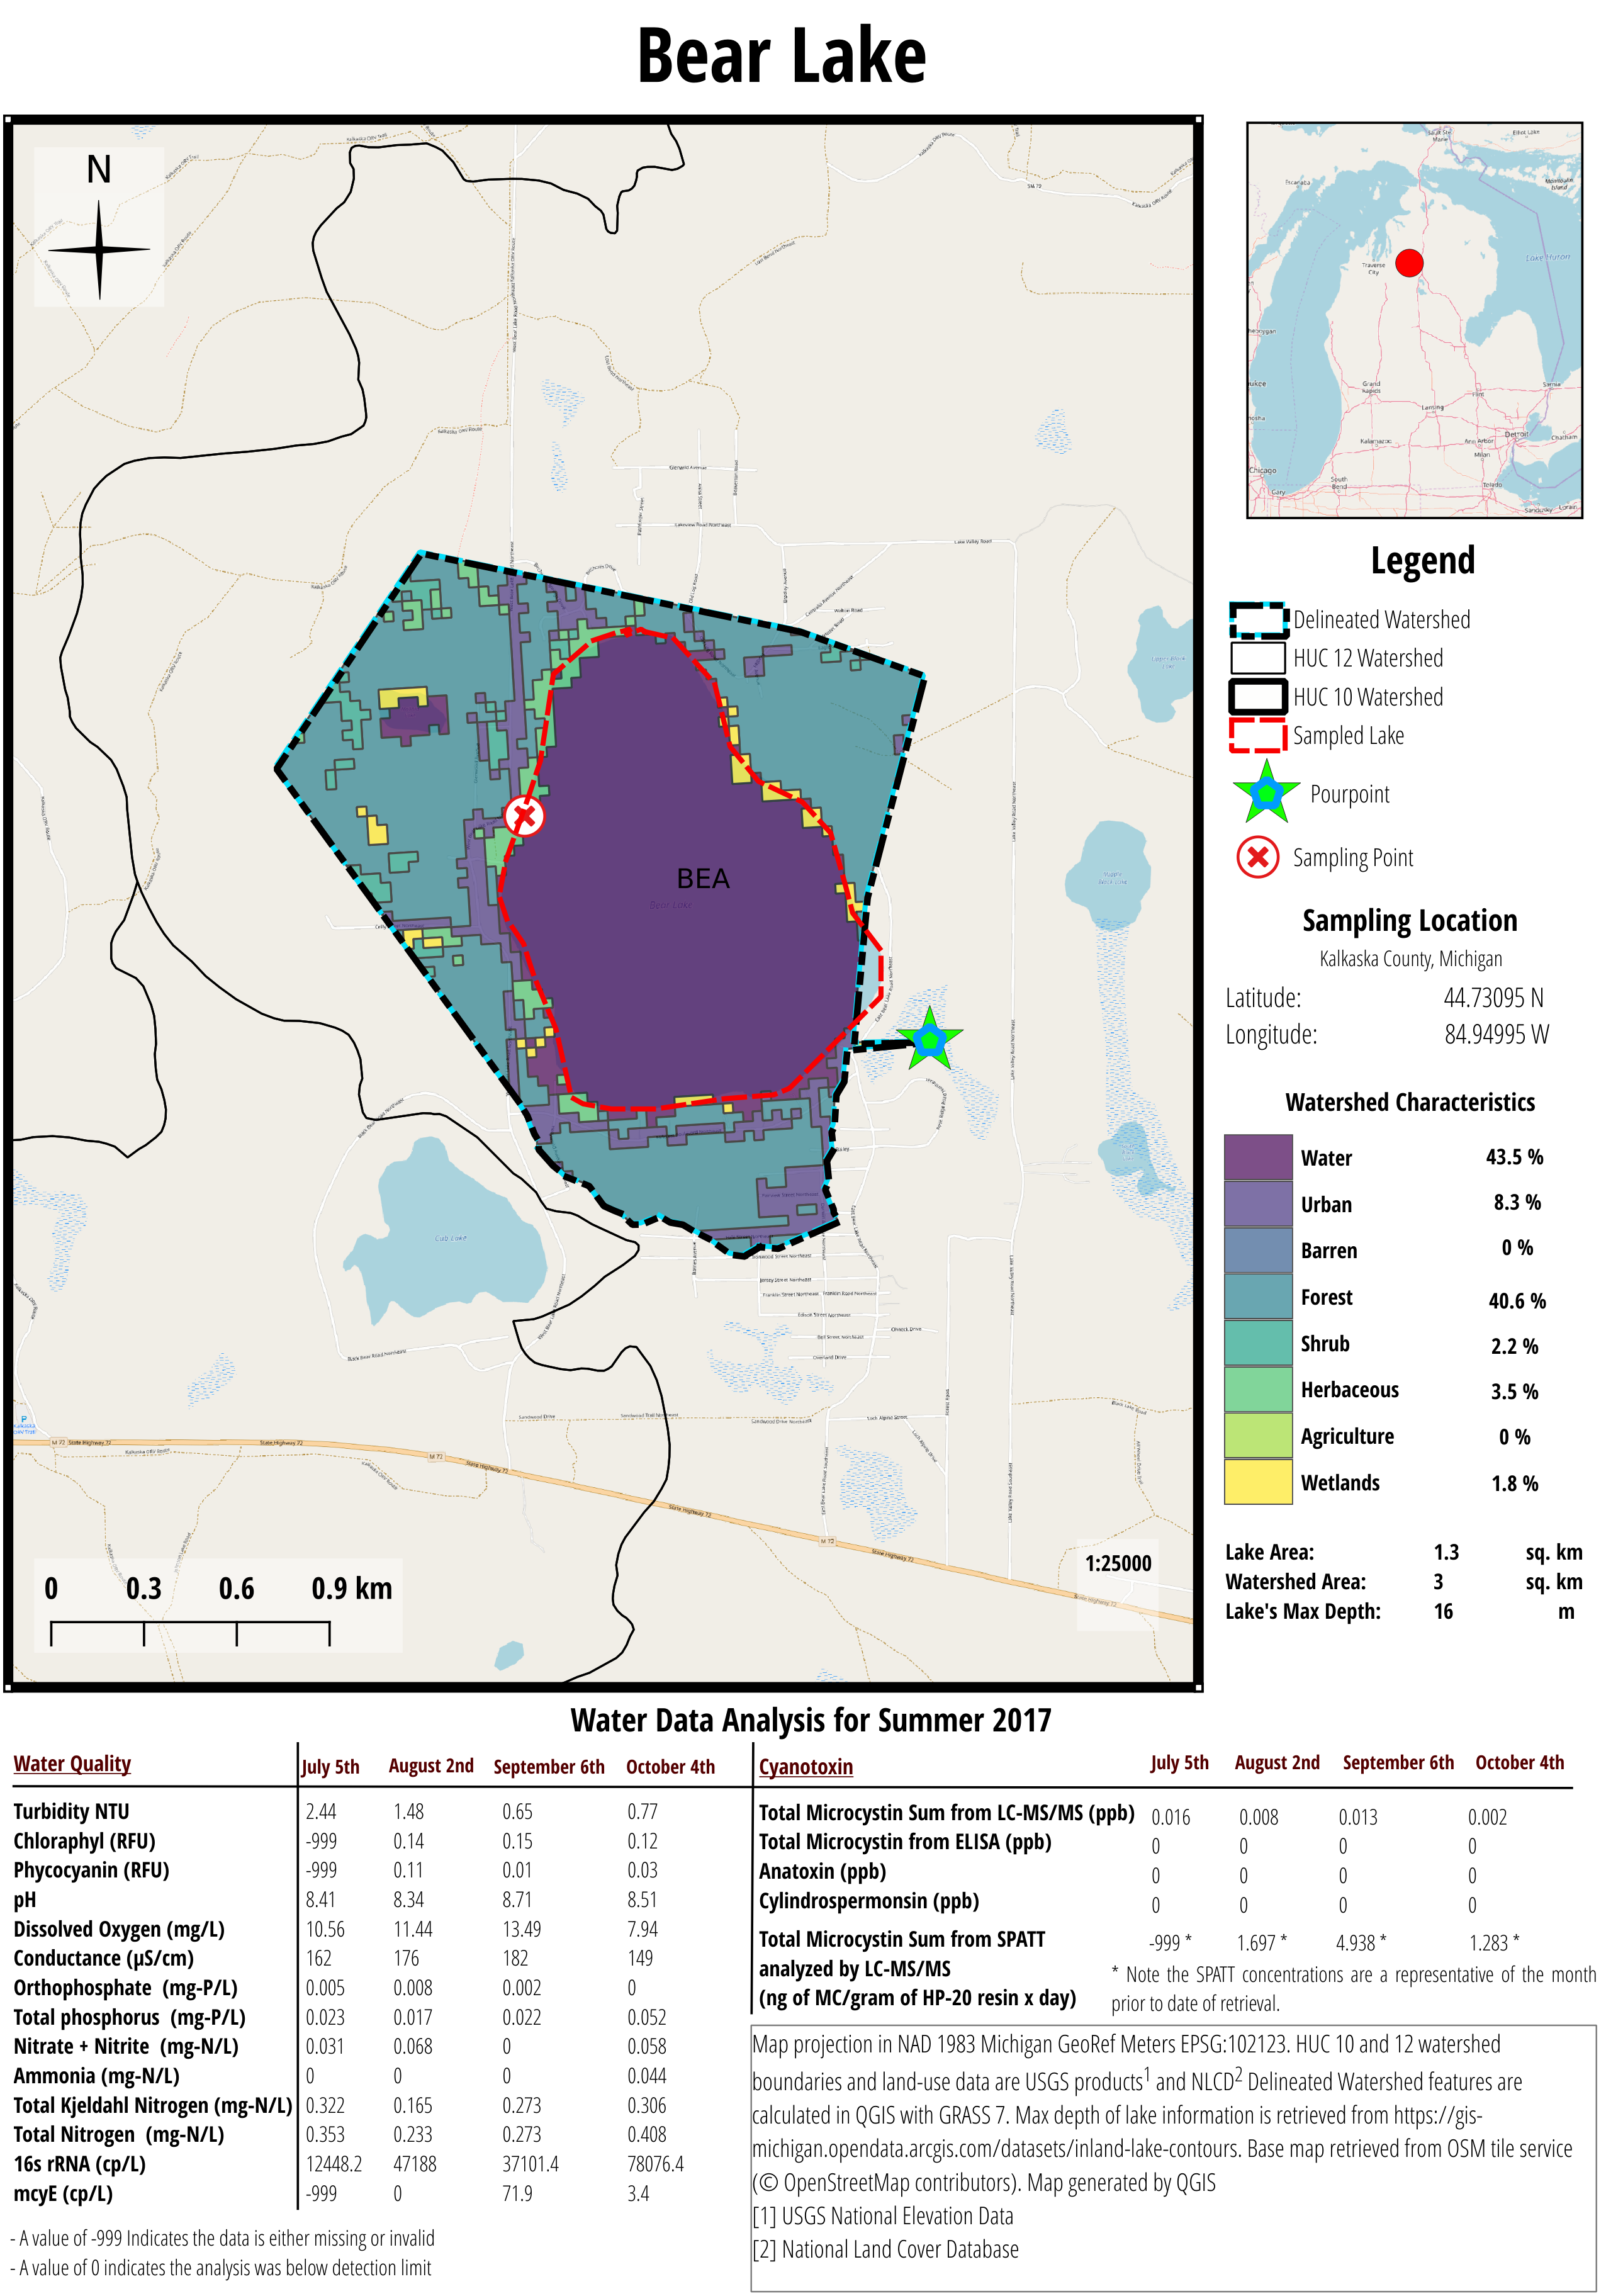
\includegraphics{figures/atlas/output_1}}
  }
\caption{GIS Map of Bear Lake}
\end{figure}

\begin{figure}[t]
\centerline{%
  \resizebox{\textwidth}{!}{\includegraphics{figures/atlas/output_2}}
  }
\caption{GIS Map of Belleville Lake}
\end{figure}

\begin{figure}[t]
\centerline{%
  \resizebox{\textwidth}{!}{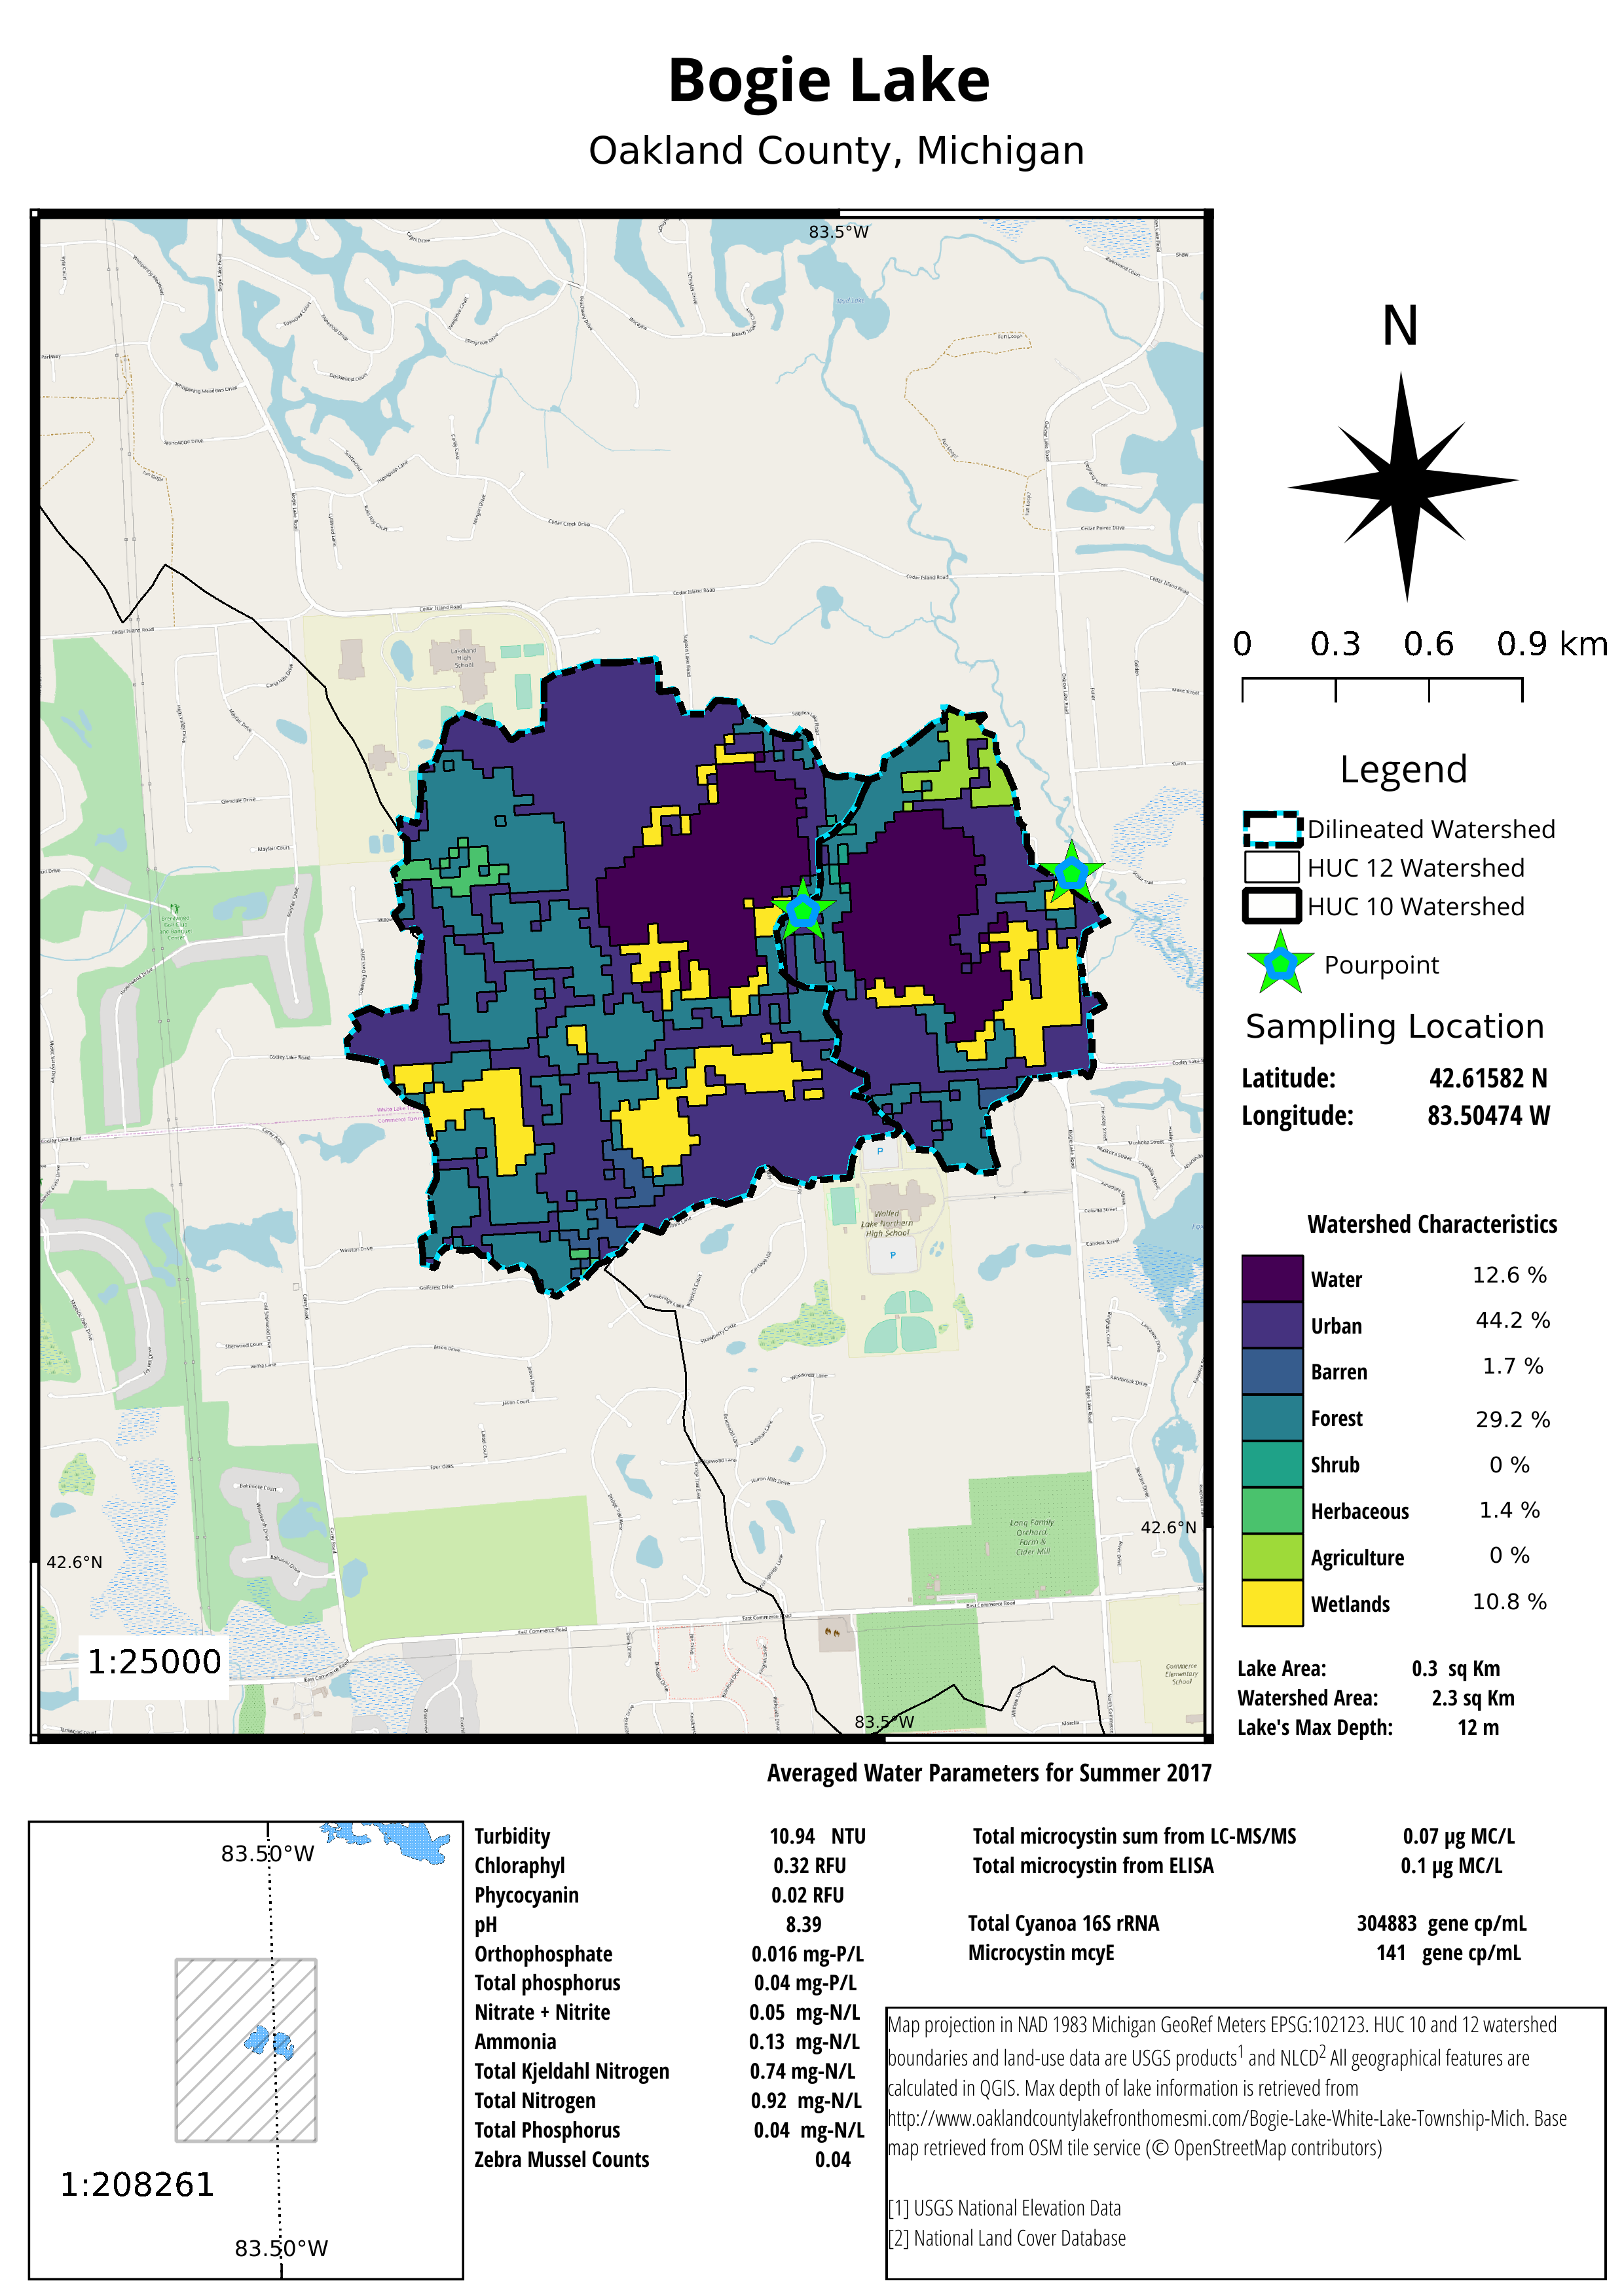
\includegraphics{figures/atlas/output_3}}
  }
\caption{GIS Map of Bogie Lake}
\end{figure}

\begin{figure}[t]
\centerline{%
  \resizebox{\textwidth}{!}{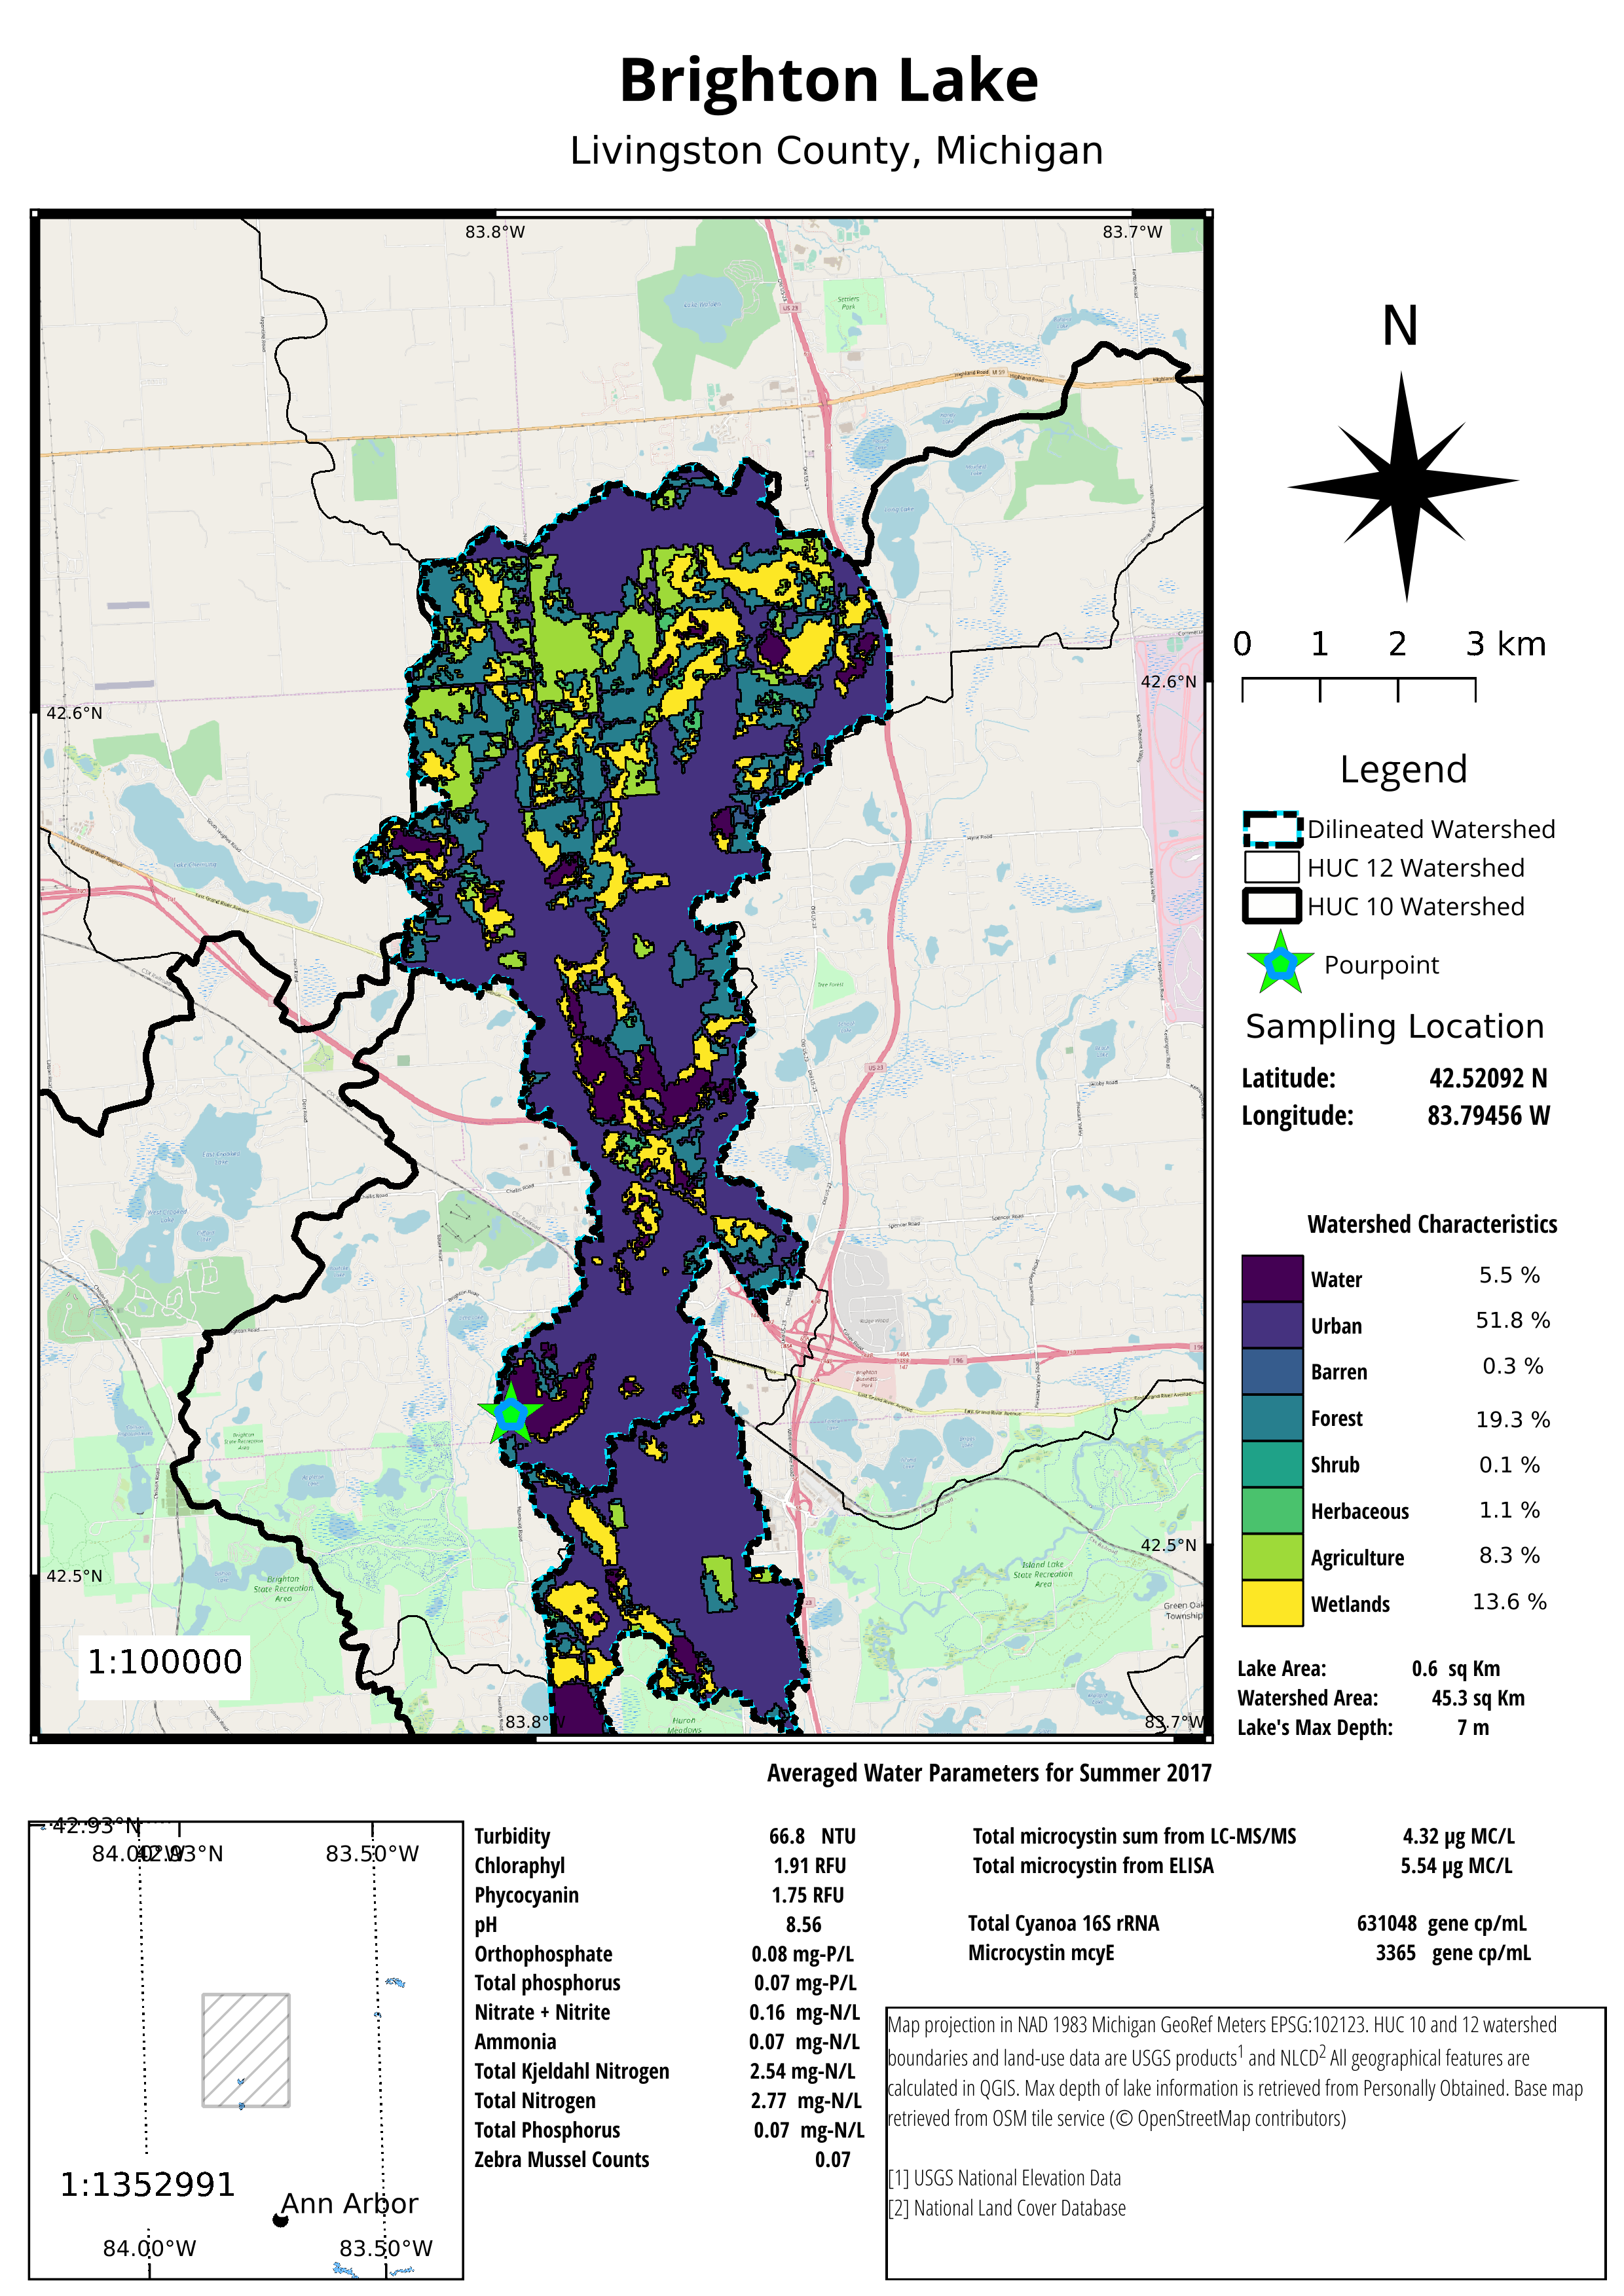
\includegraphics{figures/atlas/output_4}}
  }
\caption{GIS Map of Brighton Lake}
\end{figure}

\begin{figure}[t]
\centerline{%
  \resizebox{\textwidth}{!}{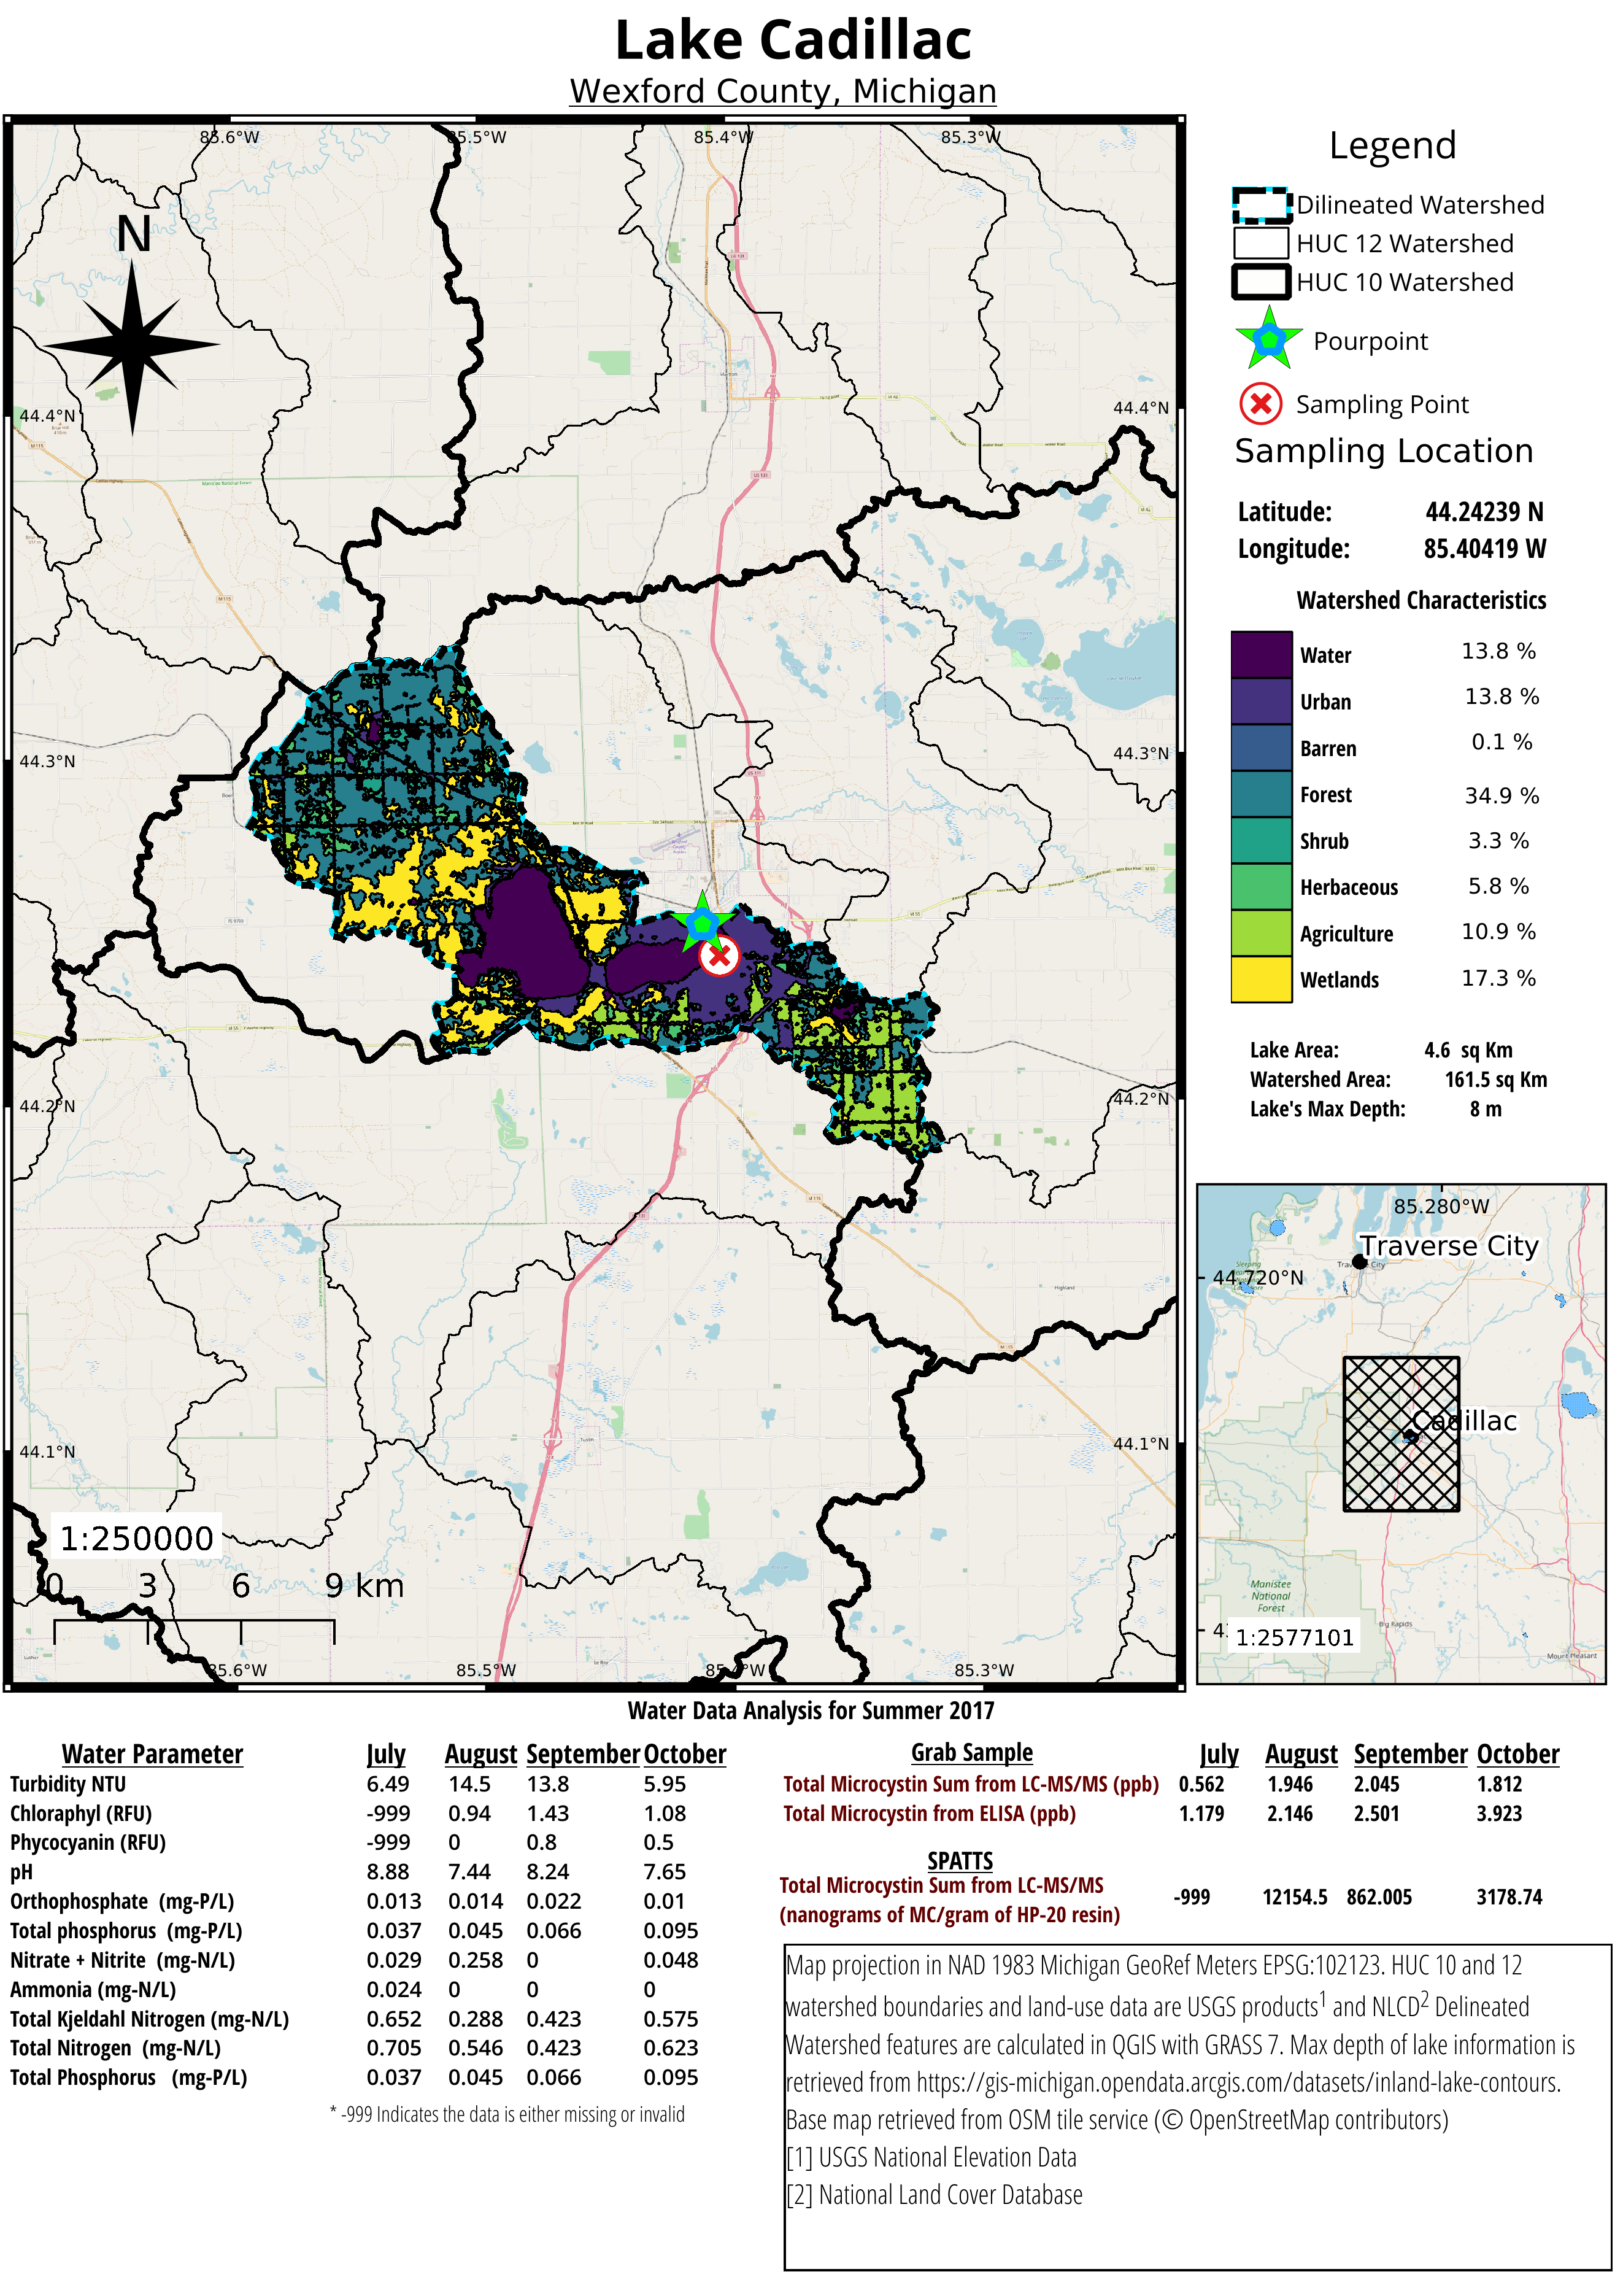
\includegraphics{figures/atlas/output_5}}
  }
\caption{GIS Map of Lake Cadillac}
\end{figure}

\begin{figure}[t]
\centerline{%
  \resizebox{\textwidth}{!}{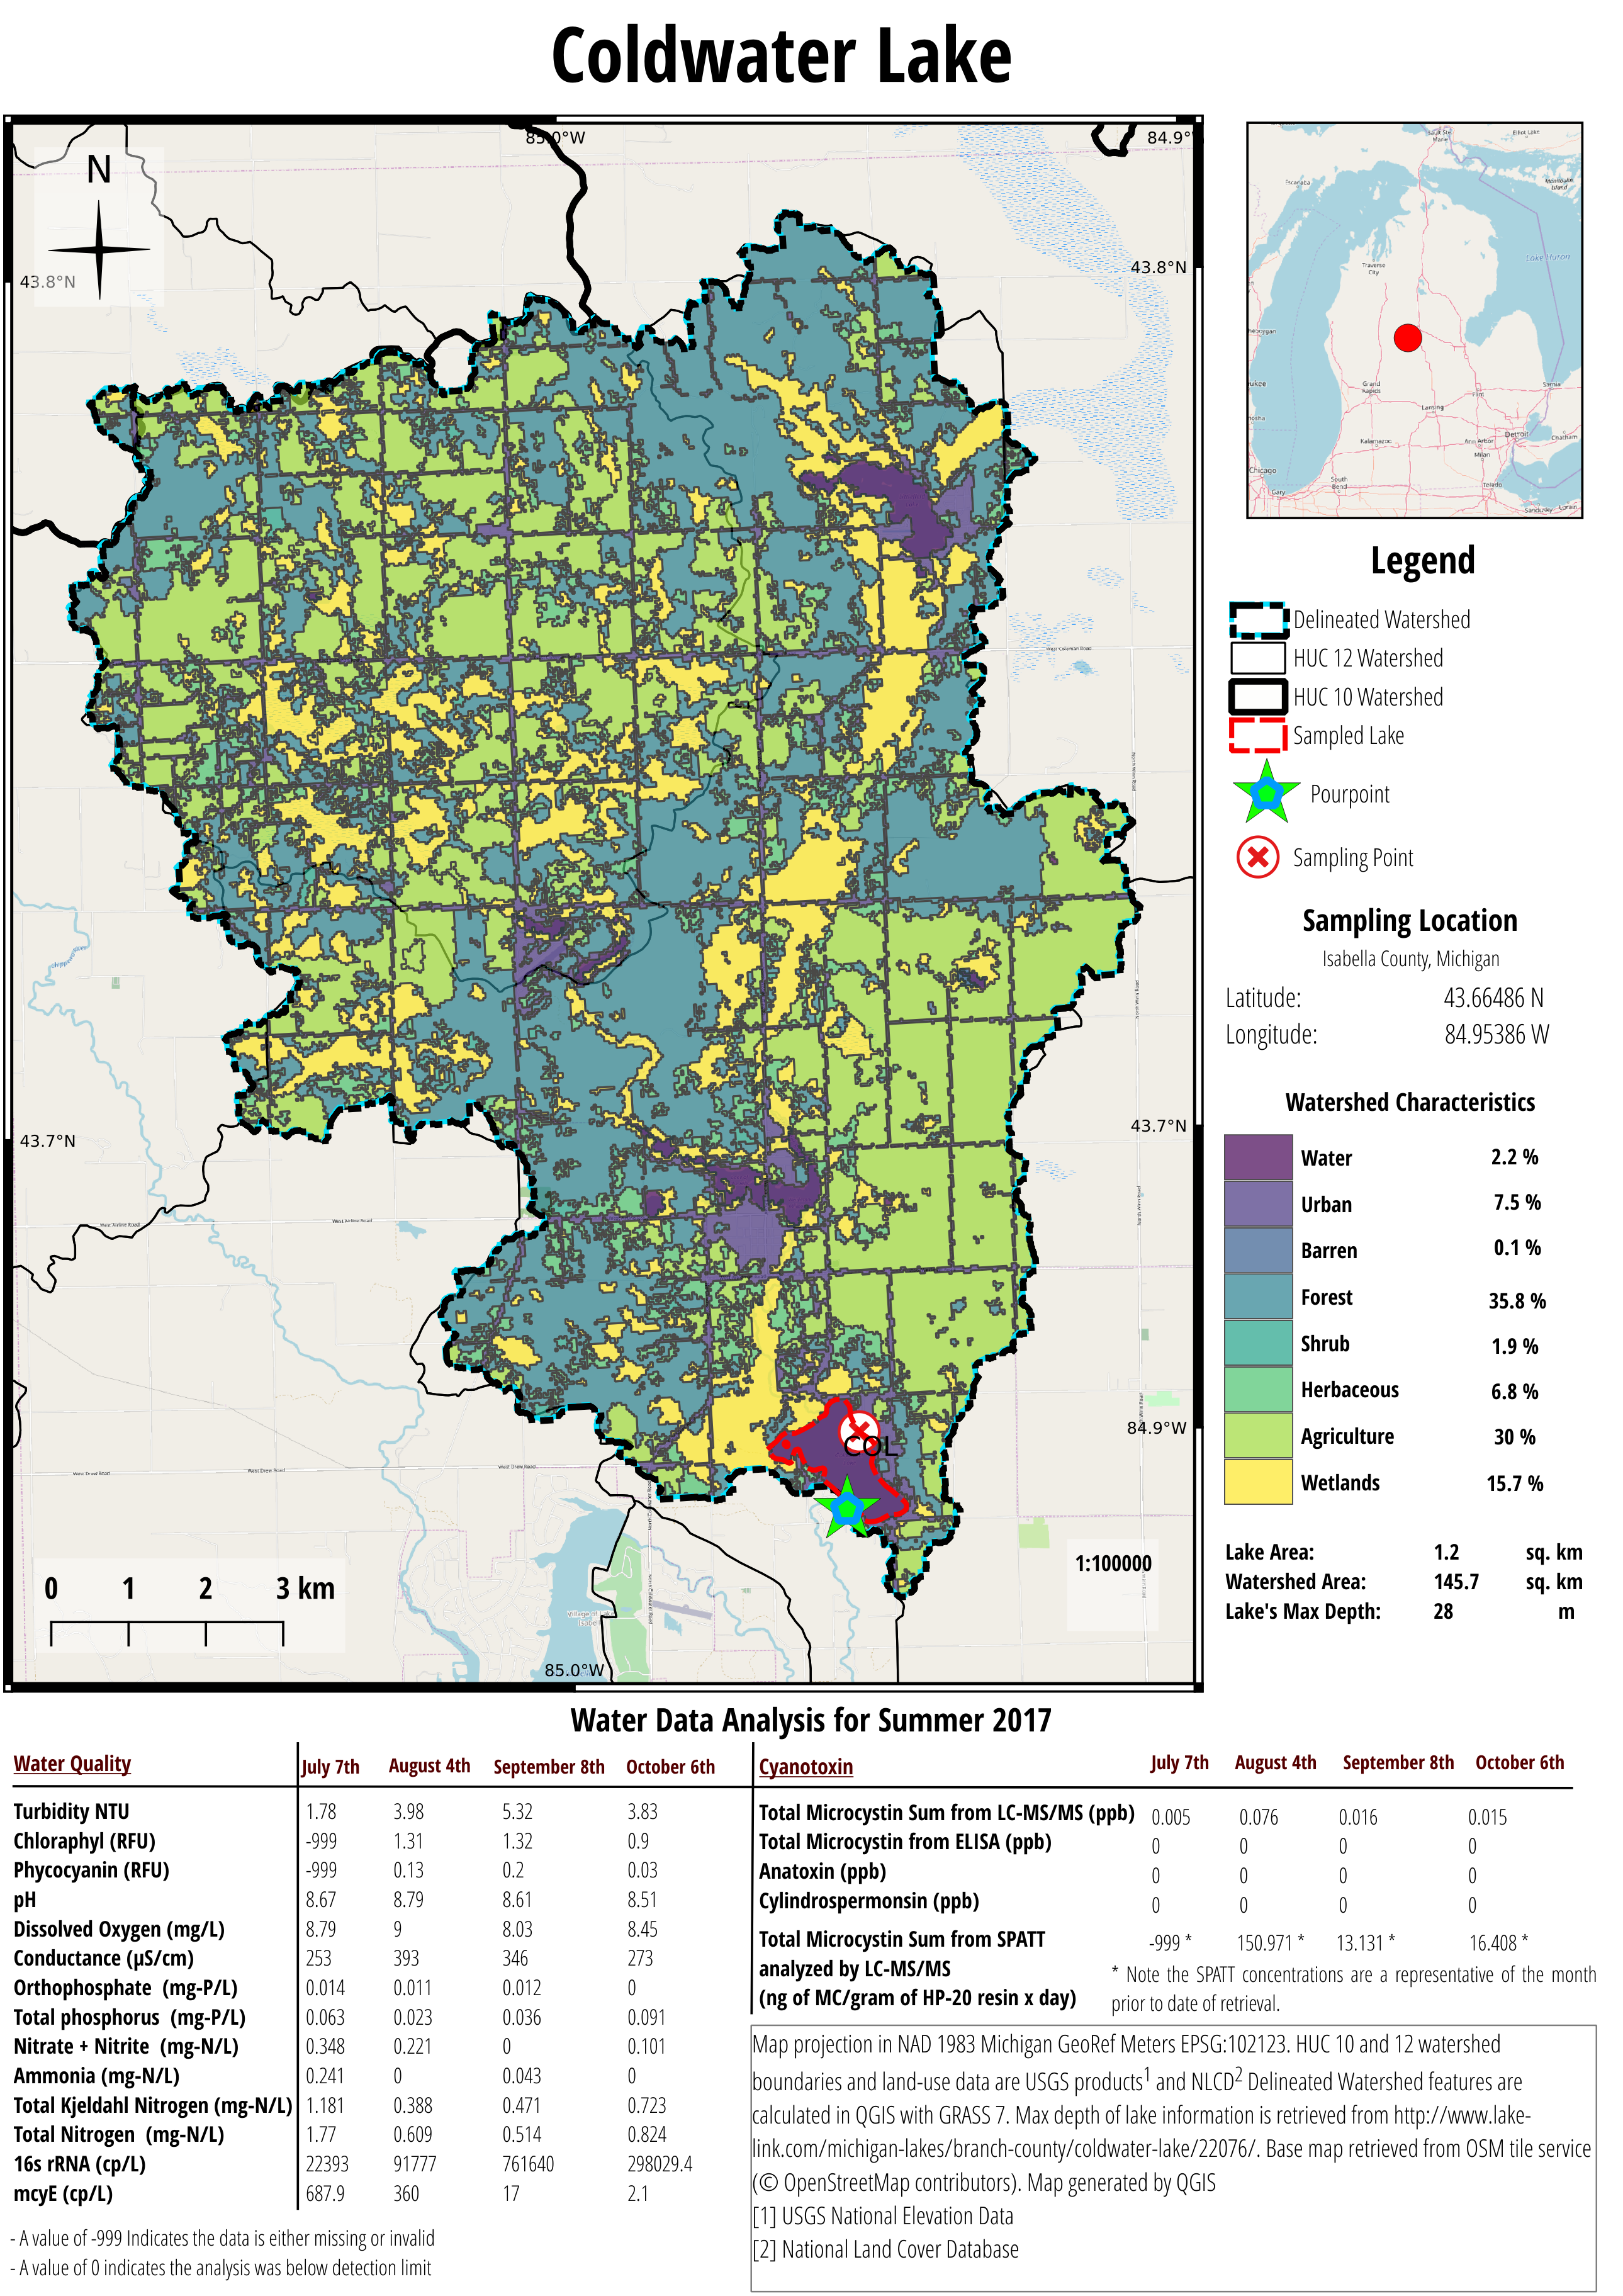
\includegraphics{figures/atlas/output_6}}
  }
\caption{GIS Map of Coldwater Lake}
\end{figure}

\begin{figure}[t]
\centerline{%
  \resizebox{\textwidth}{!}{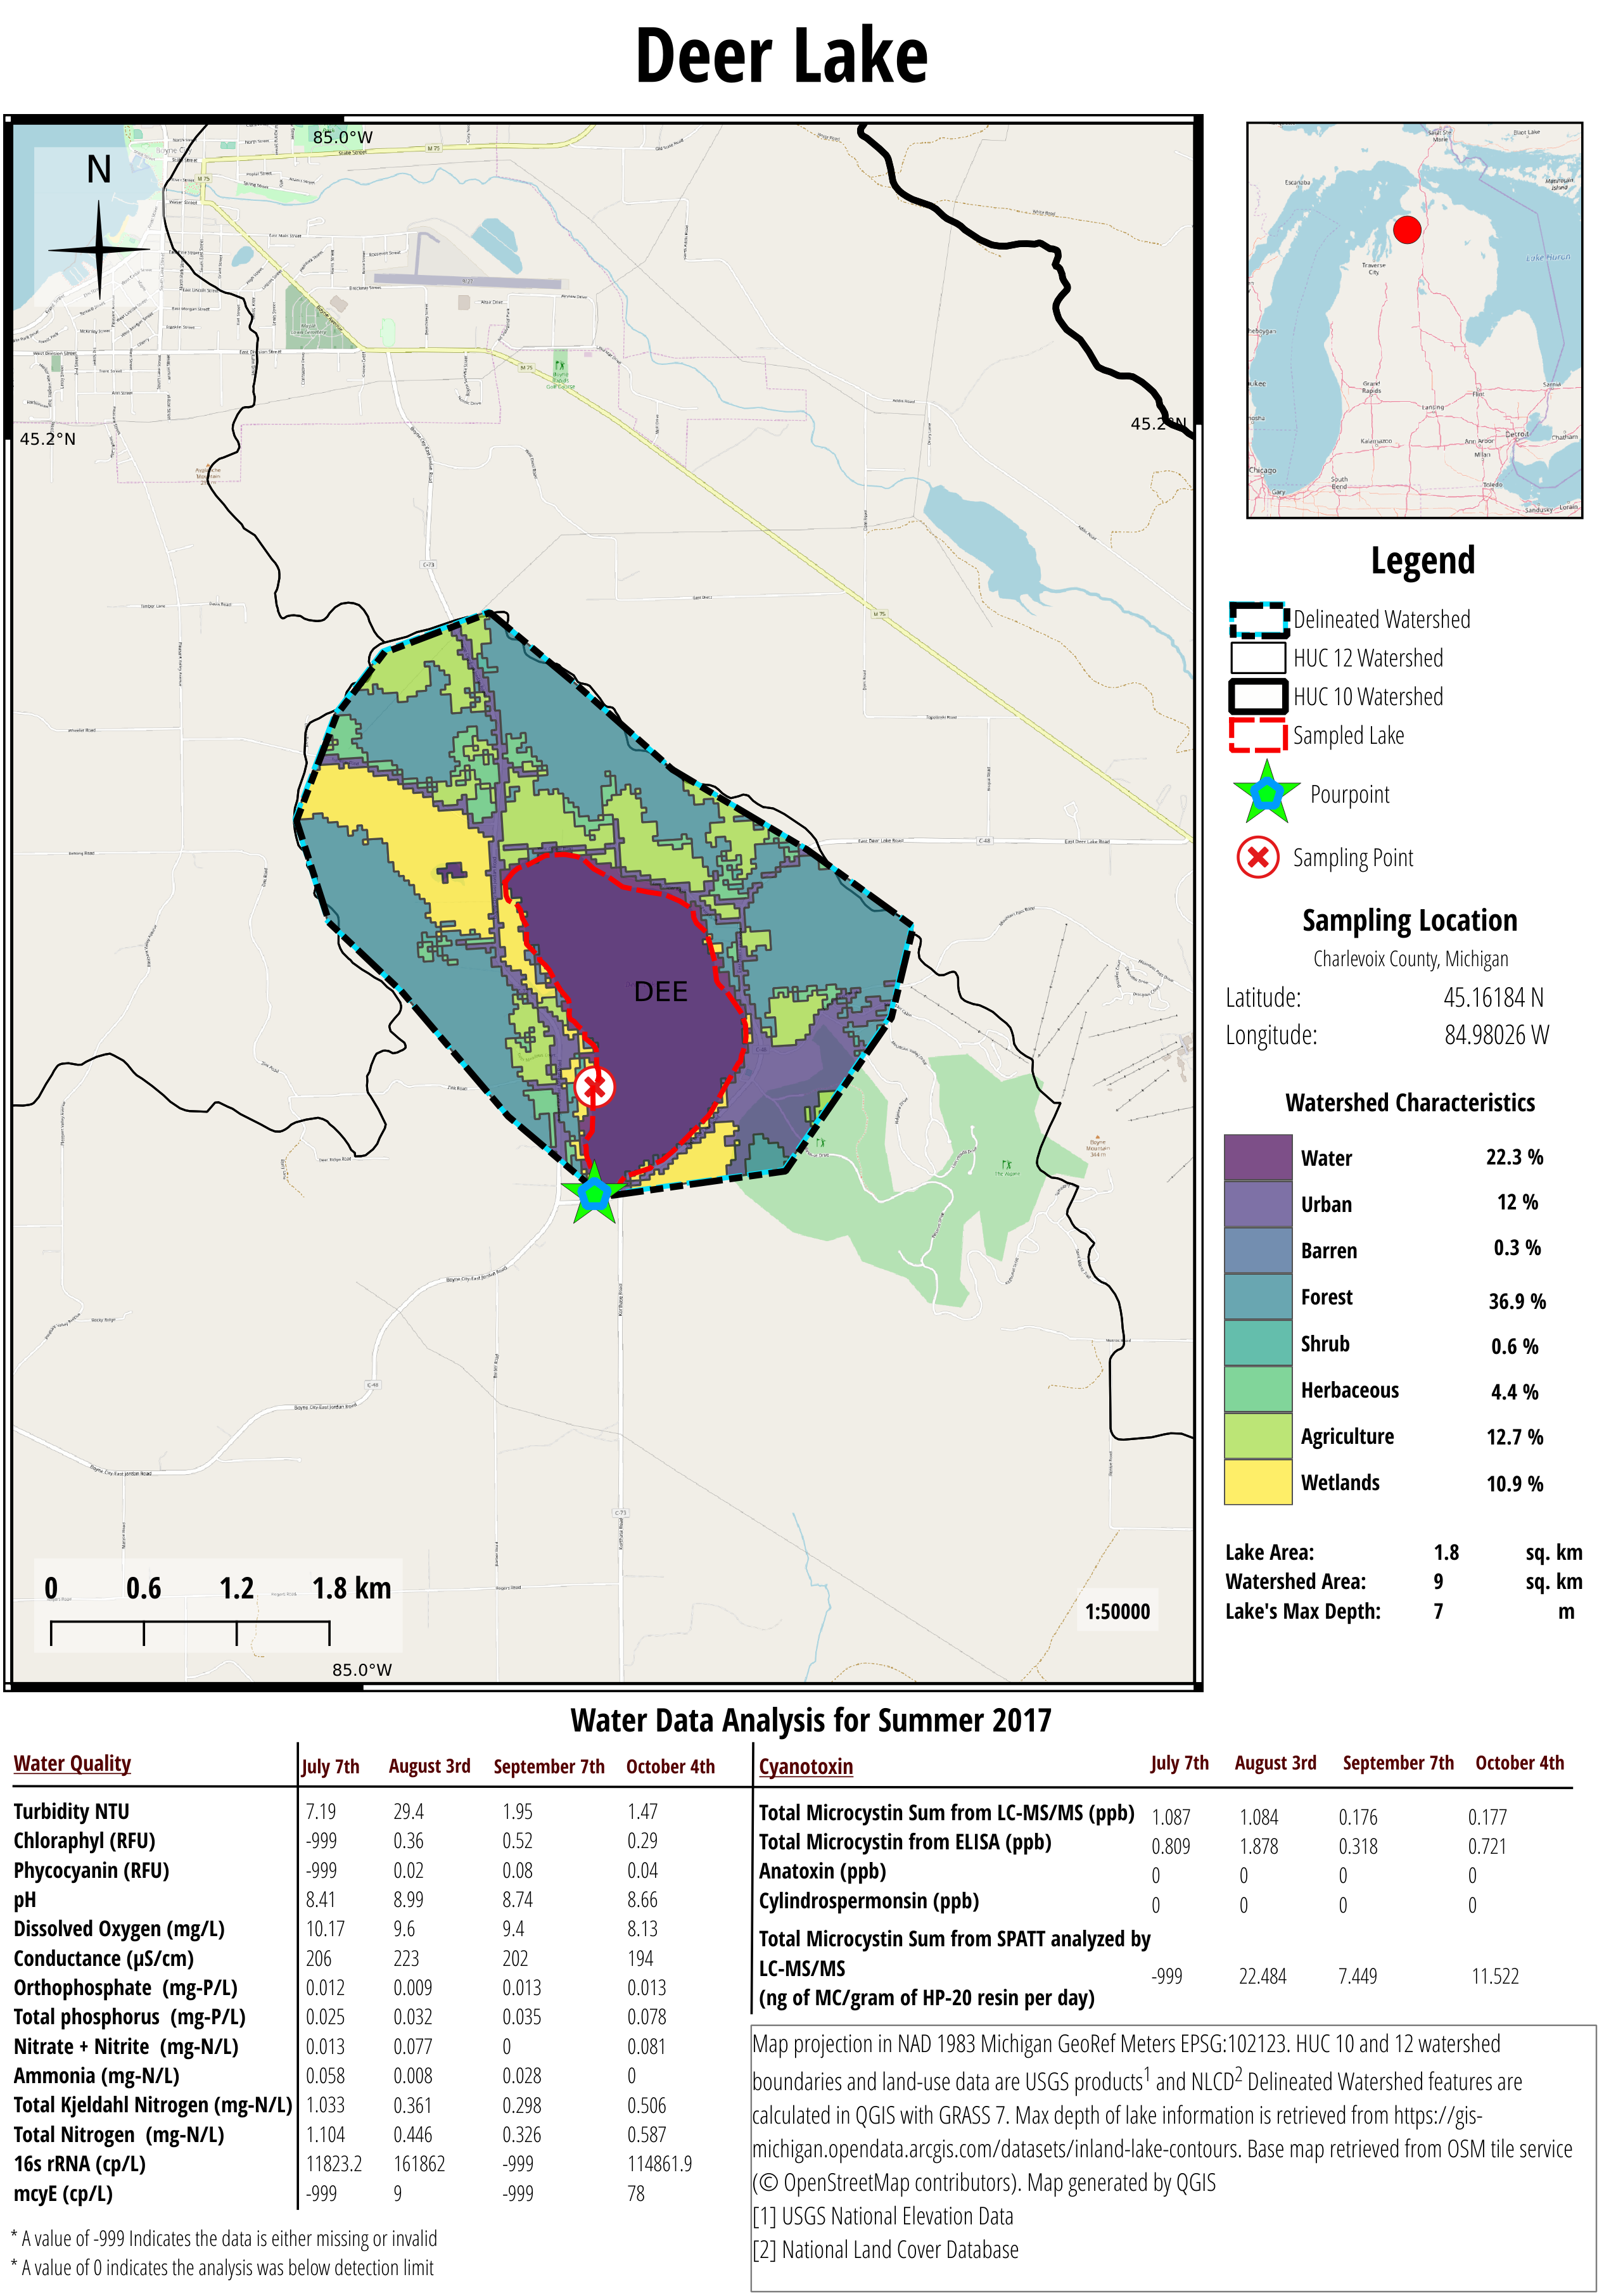
\includegraphics{figures/atlas/output_7}}
  }
\caption{GIS Map of Deer Lake}
\end{figure}

\begin{figure}[t]
\centerline{%
  \resizebox{\textwidth}{!}{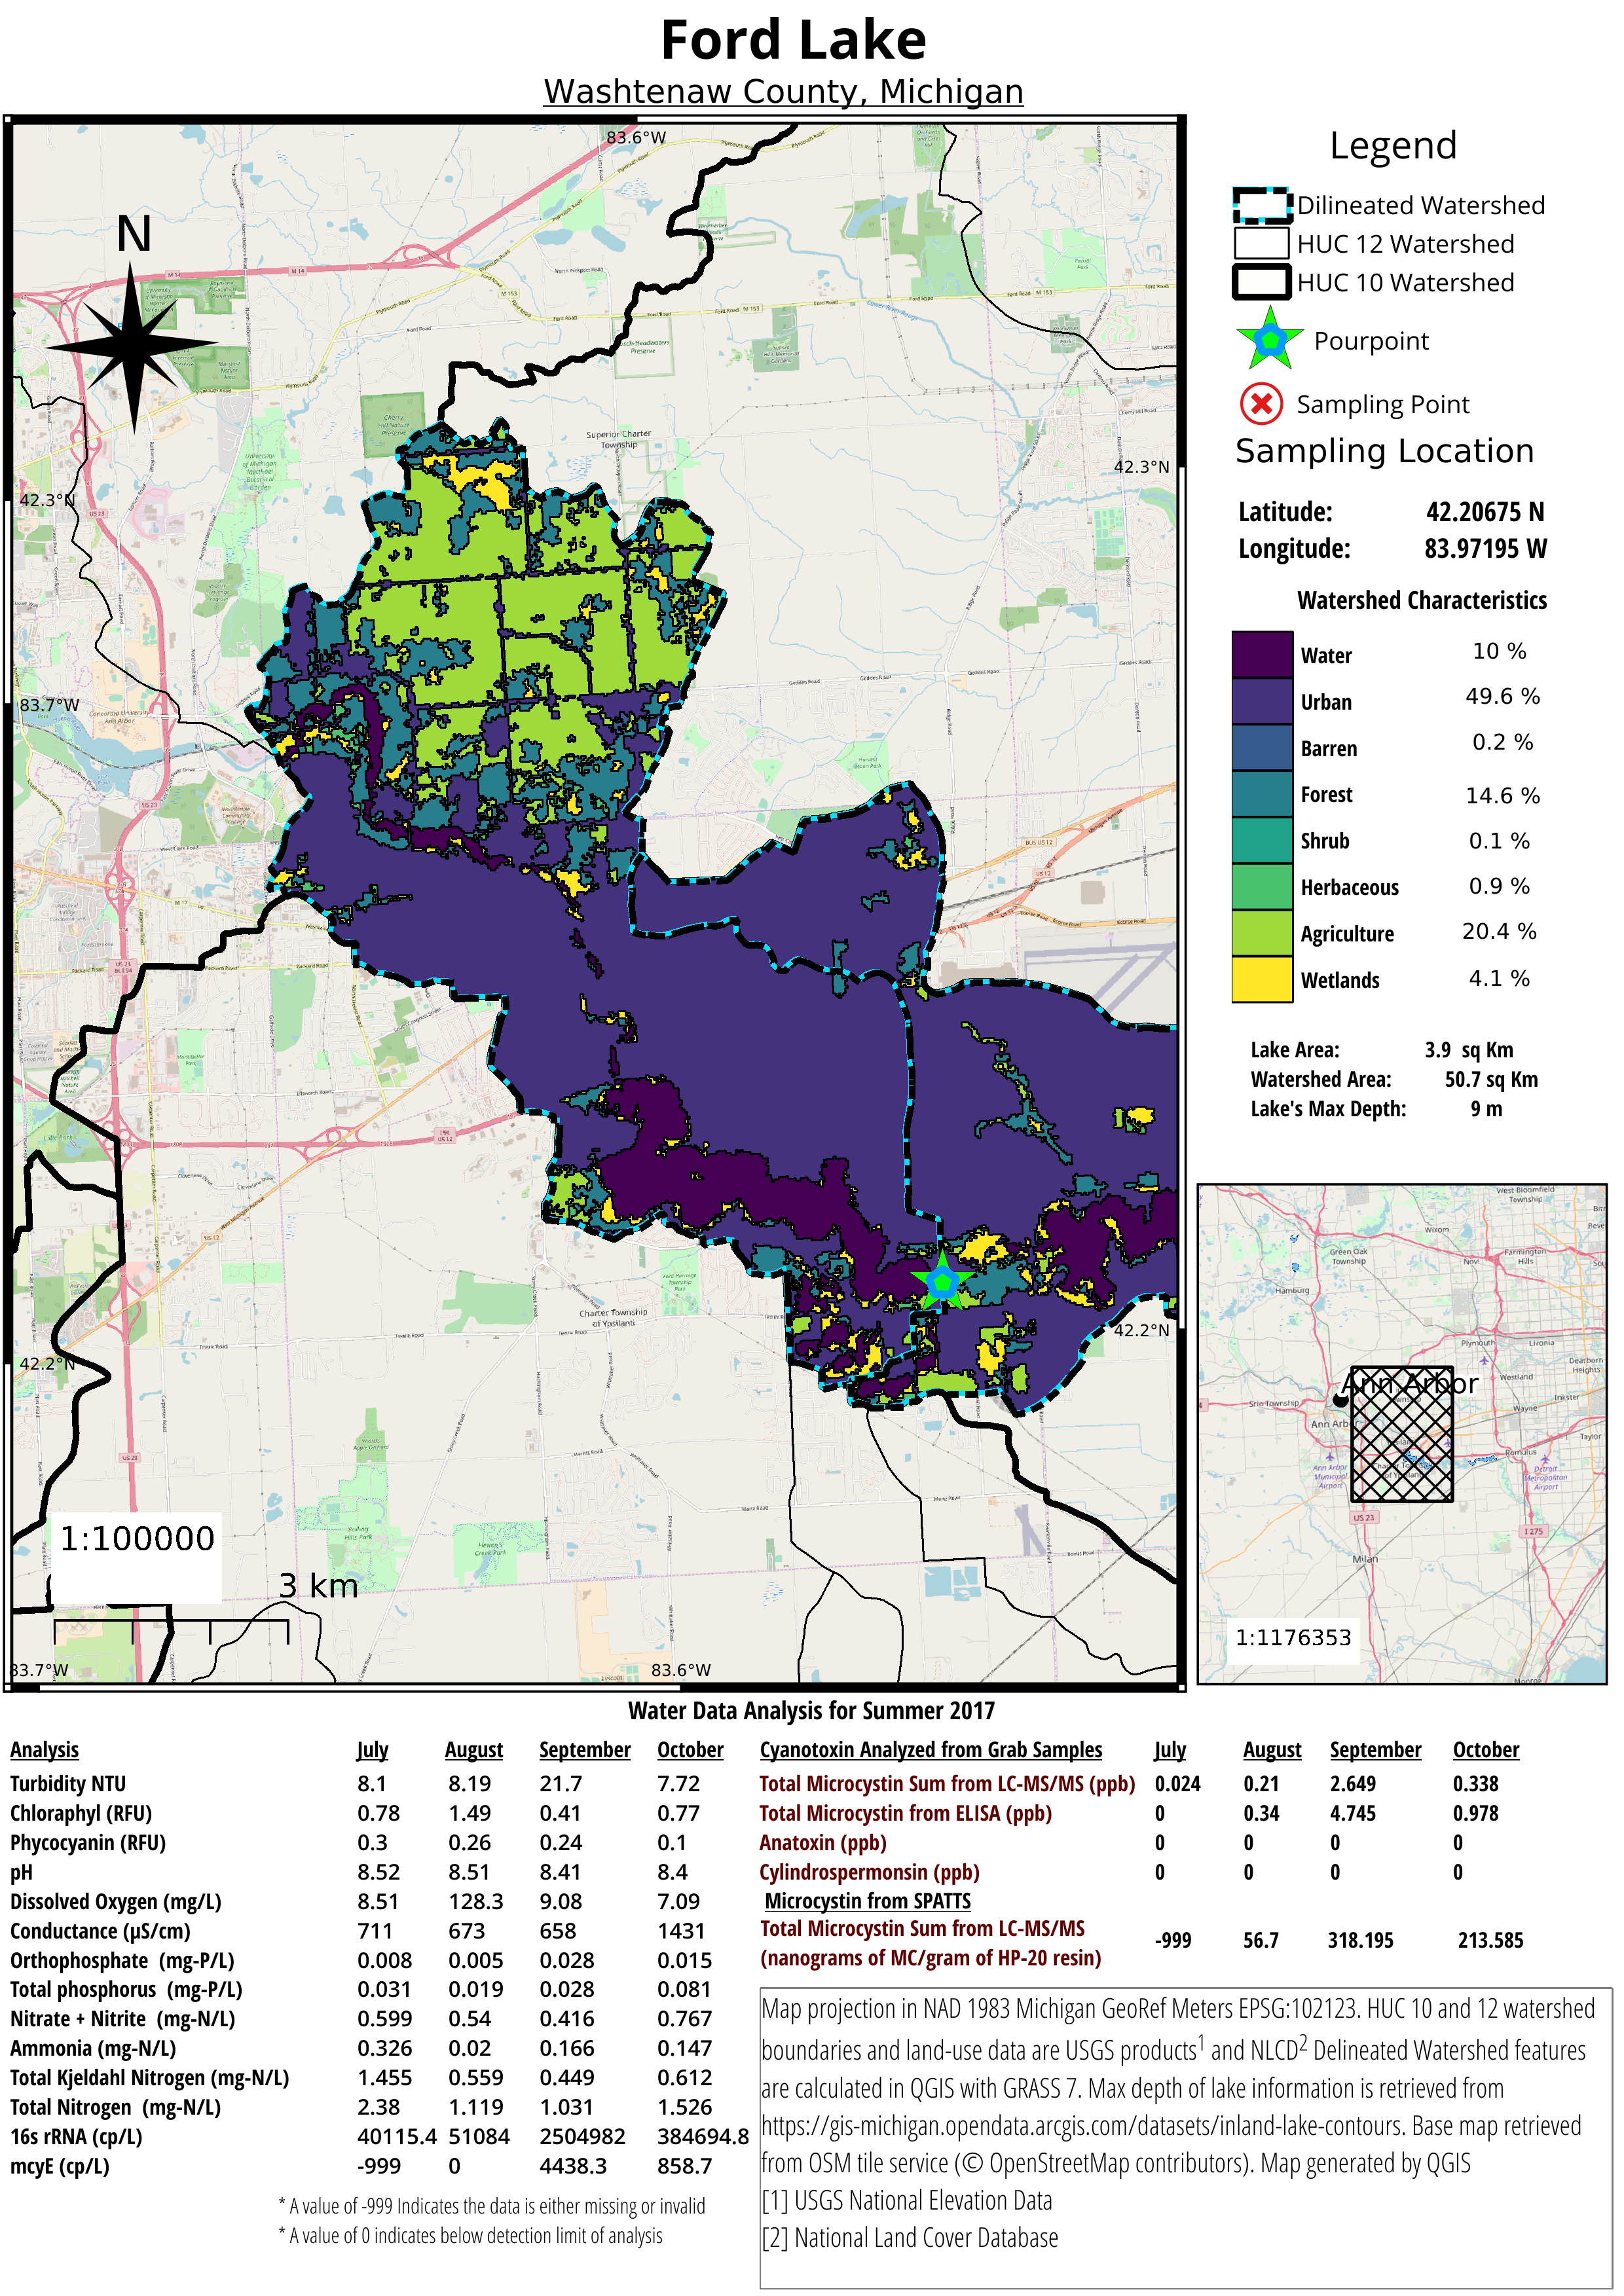
\includegraphics{figures/atlas/output_8}}
  }
\caption{GIS Map of Ford Lake}
\end{figure}

\begin{figure}[t]
\centerline{%
  \resizebox{\textwidth}{!}{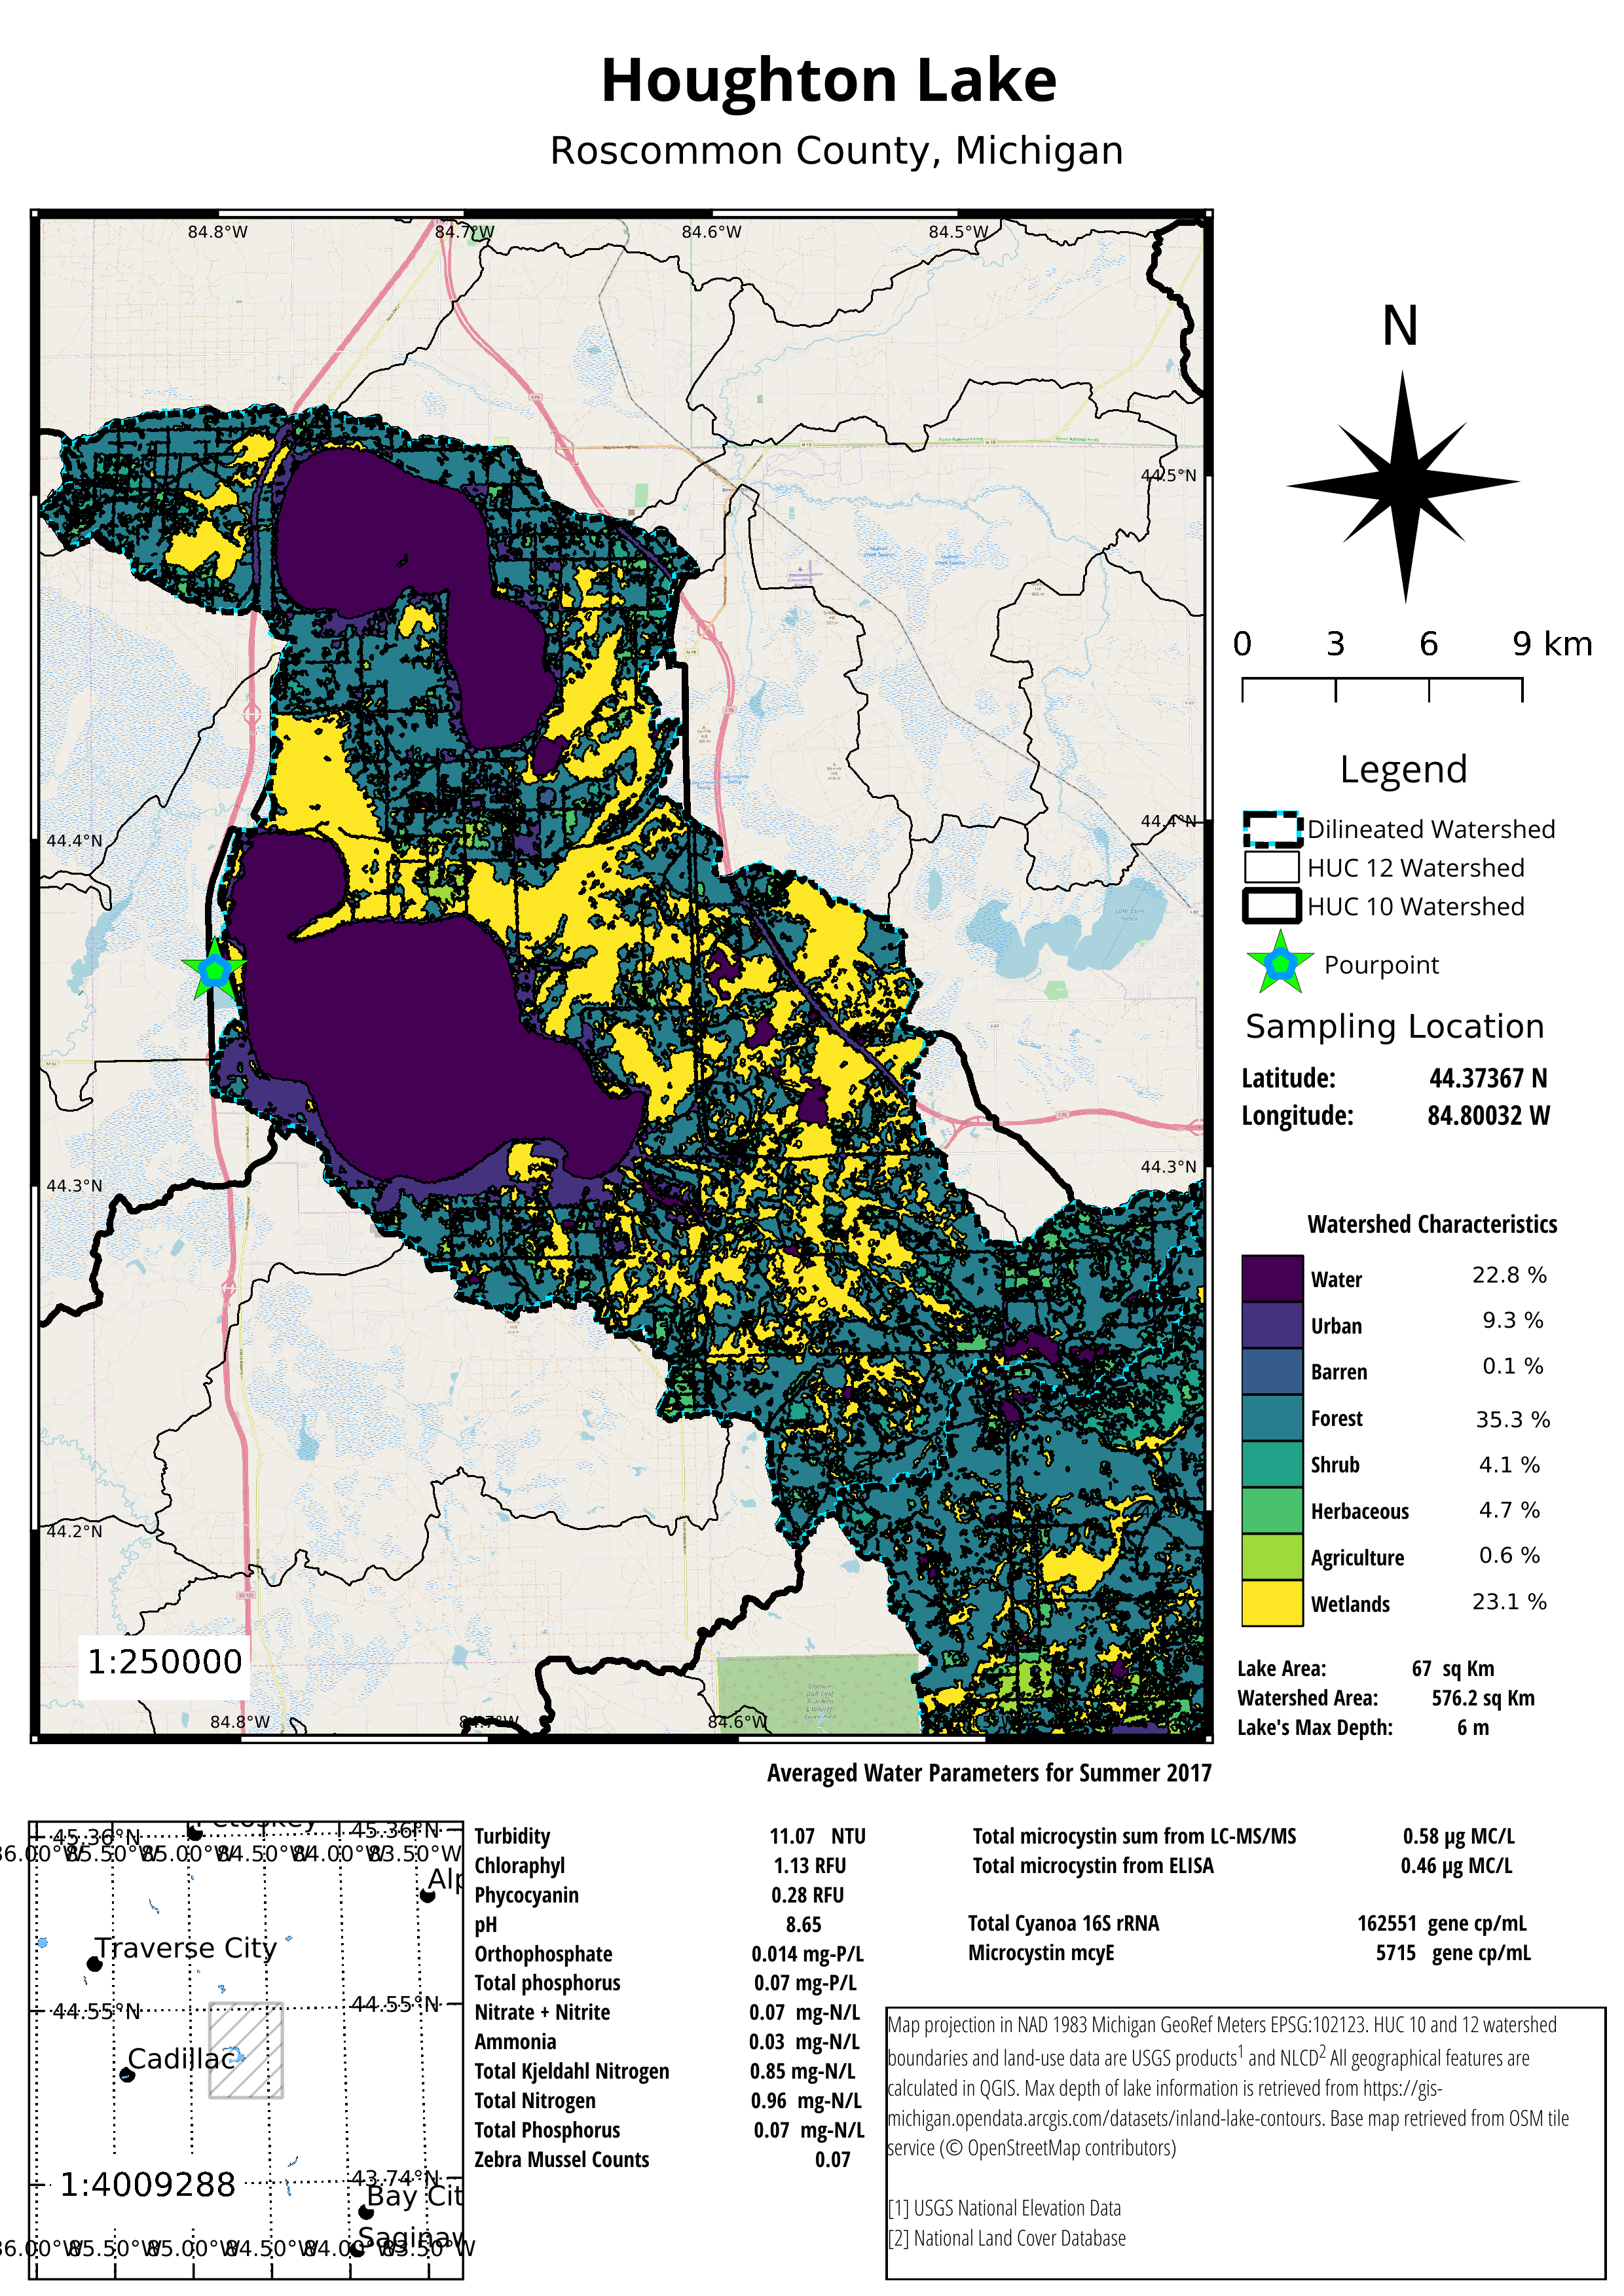
\includegraphics{figures/atlas/output_9}}
  }
\caption{GIS Map of Houghton Lake}
\end{figure}

\begin{figure}[t]
\centerline{%
  \resizebox{\textwidth}{!}{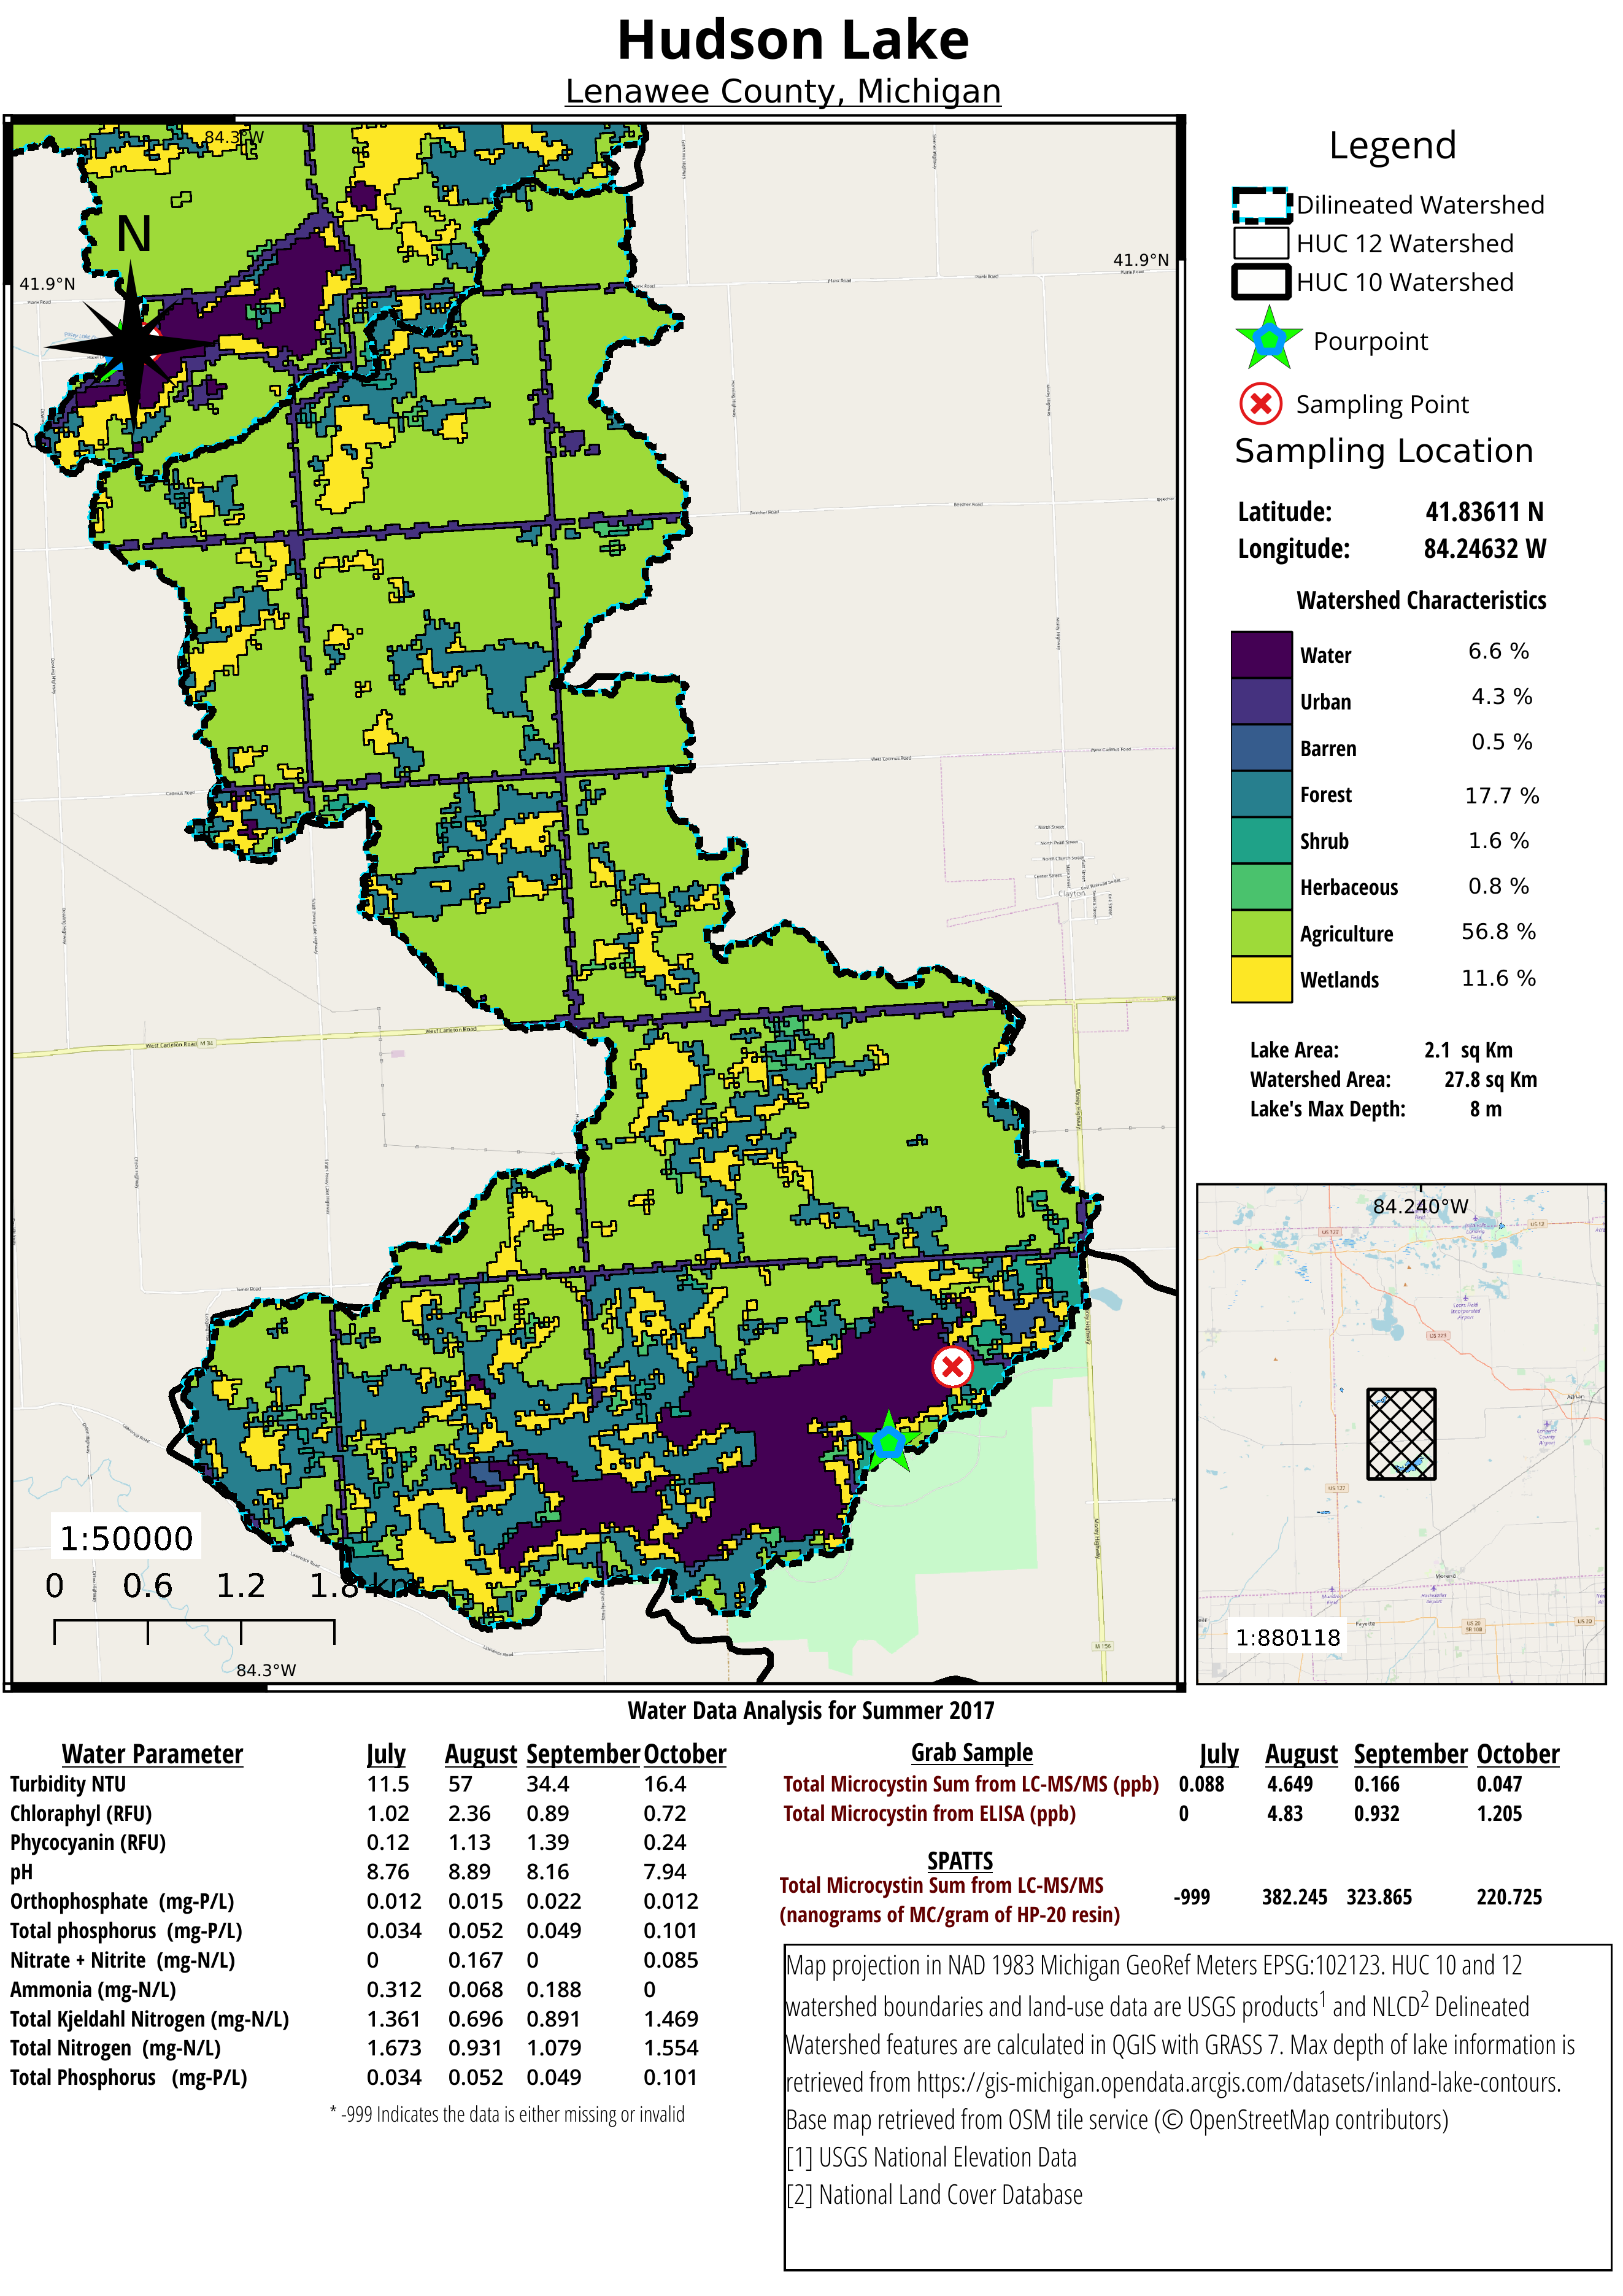
\includegraphics{figures/atlas/output_10}}
  }
\caption{GIS Map of Hudson Lake}
\end{figure}

\begin{figure}[t]
\centerline{%
  \resizebox{\textwidth}{!}{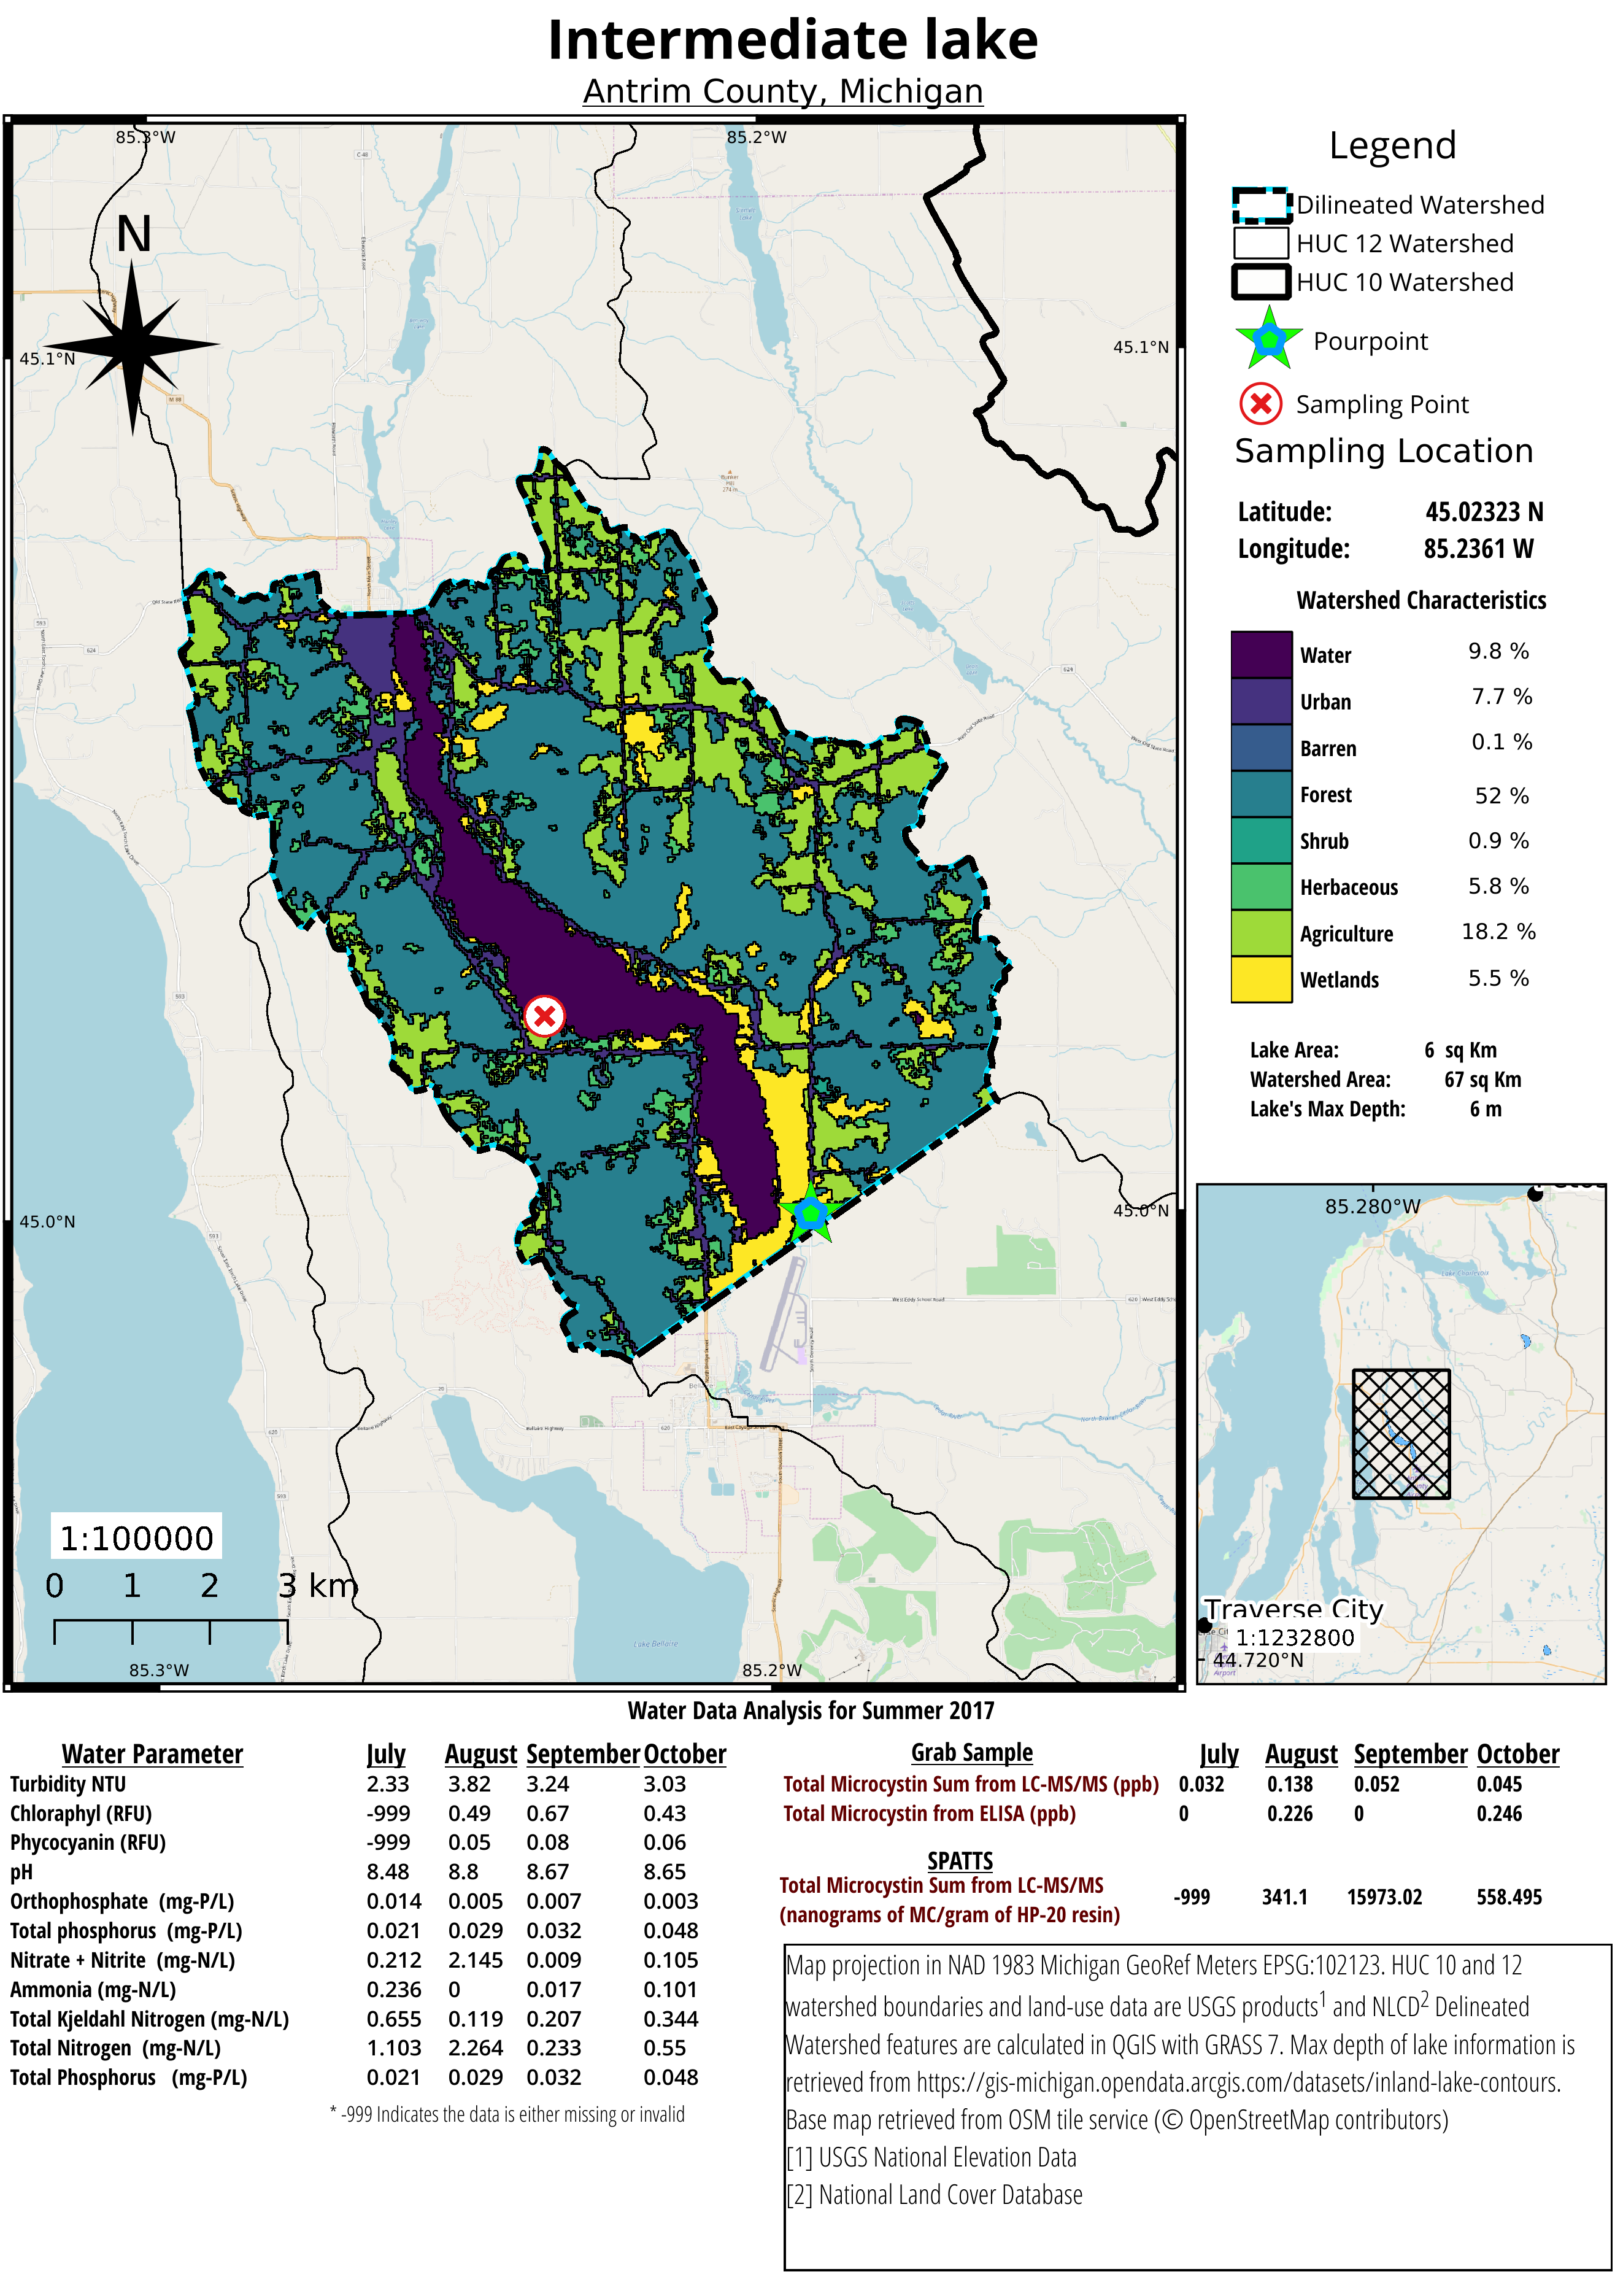
\includegraphics{figures/atlas/output_11}}
  }
\caption{GIS Map of Intermediate Lake}
\end{figure}

\begin{figure}[t]
\centerline{%
  \resizebox{\textwidth}{!}{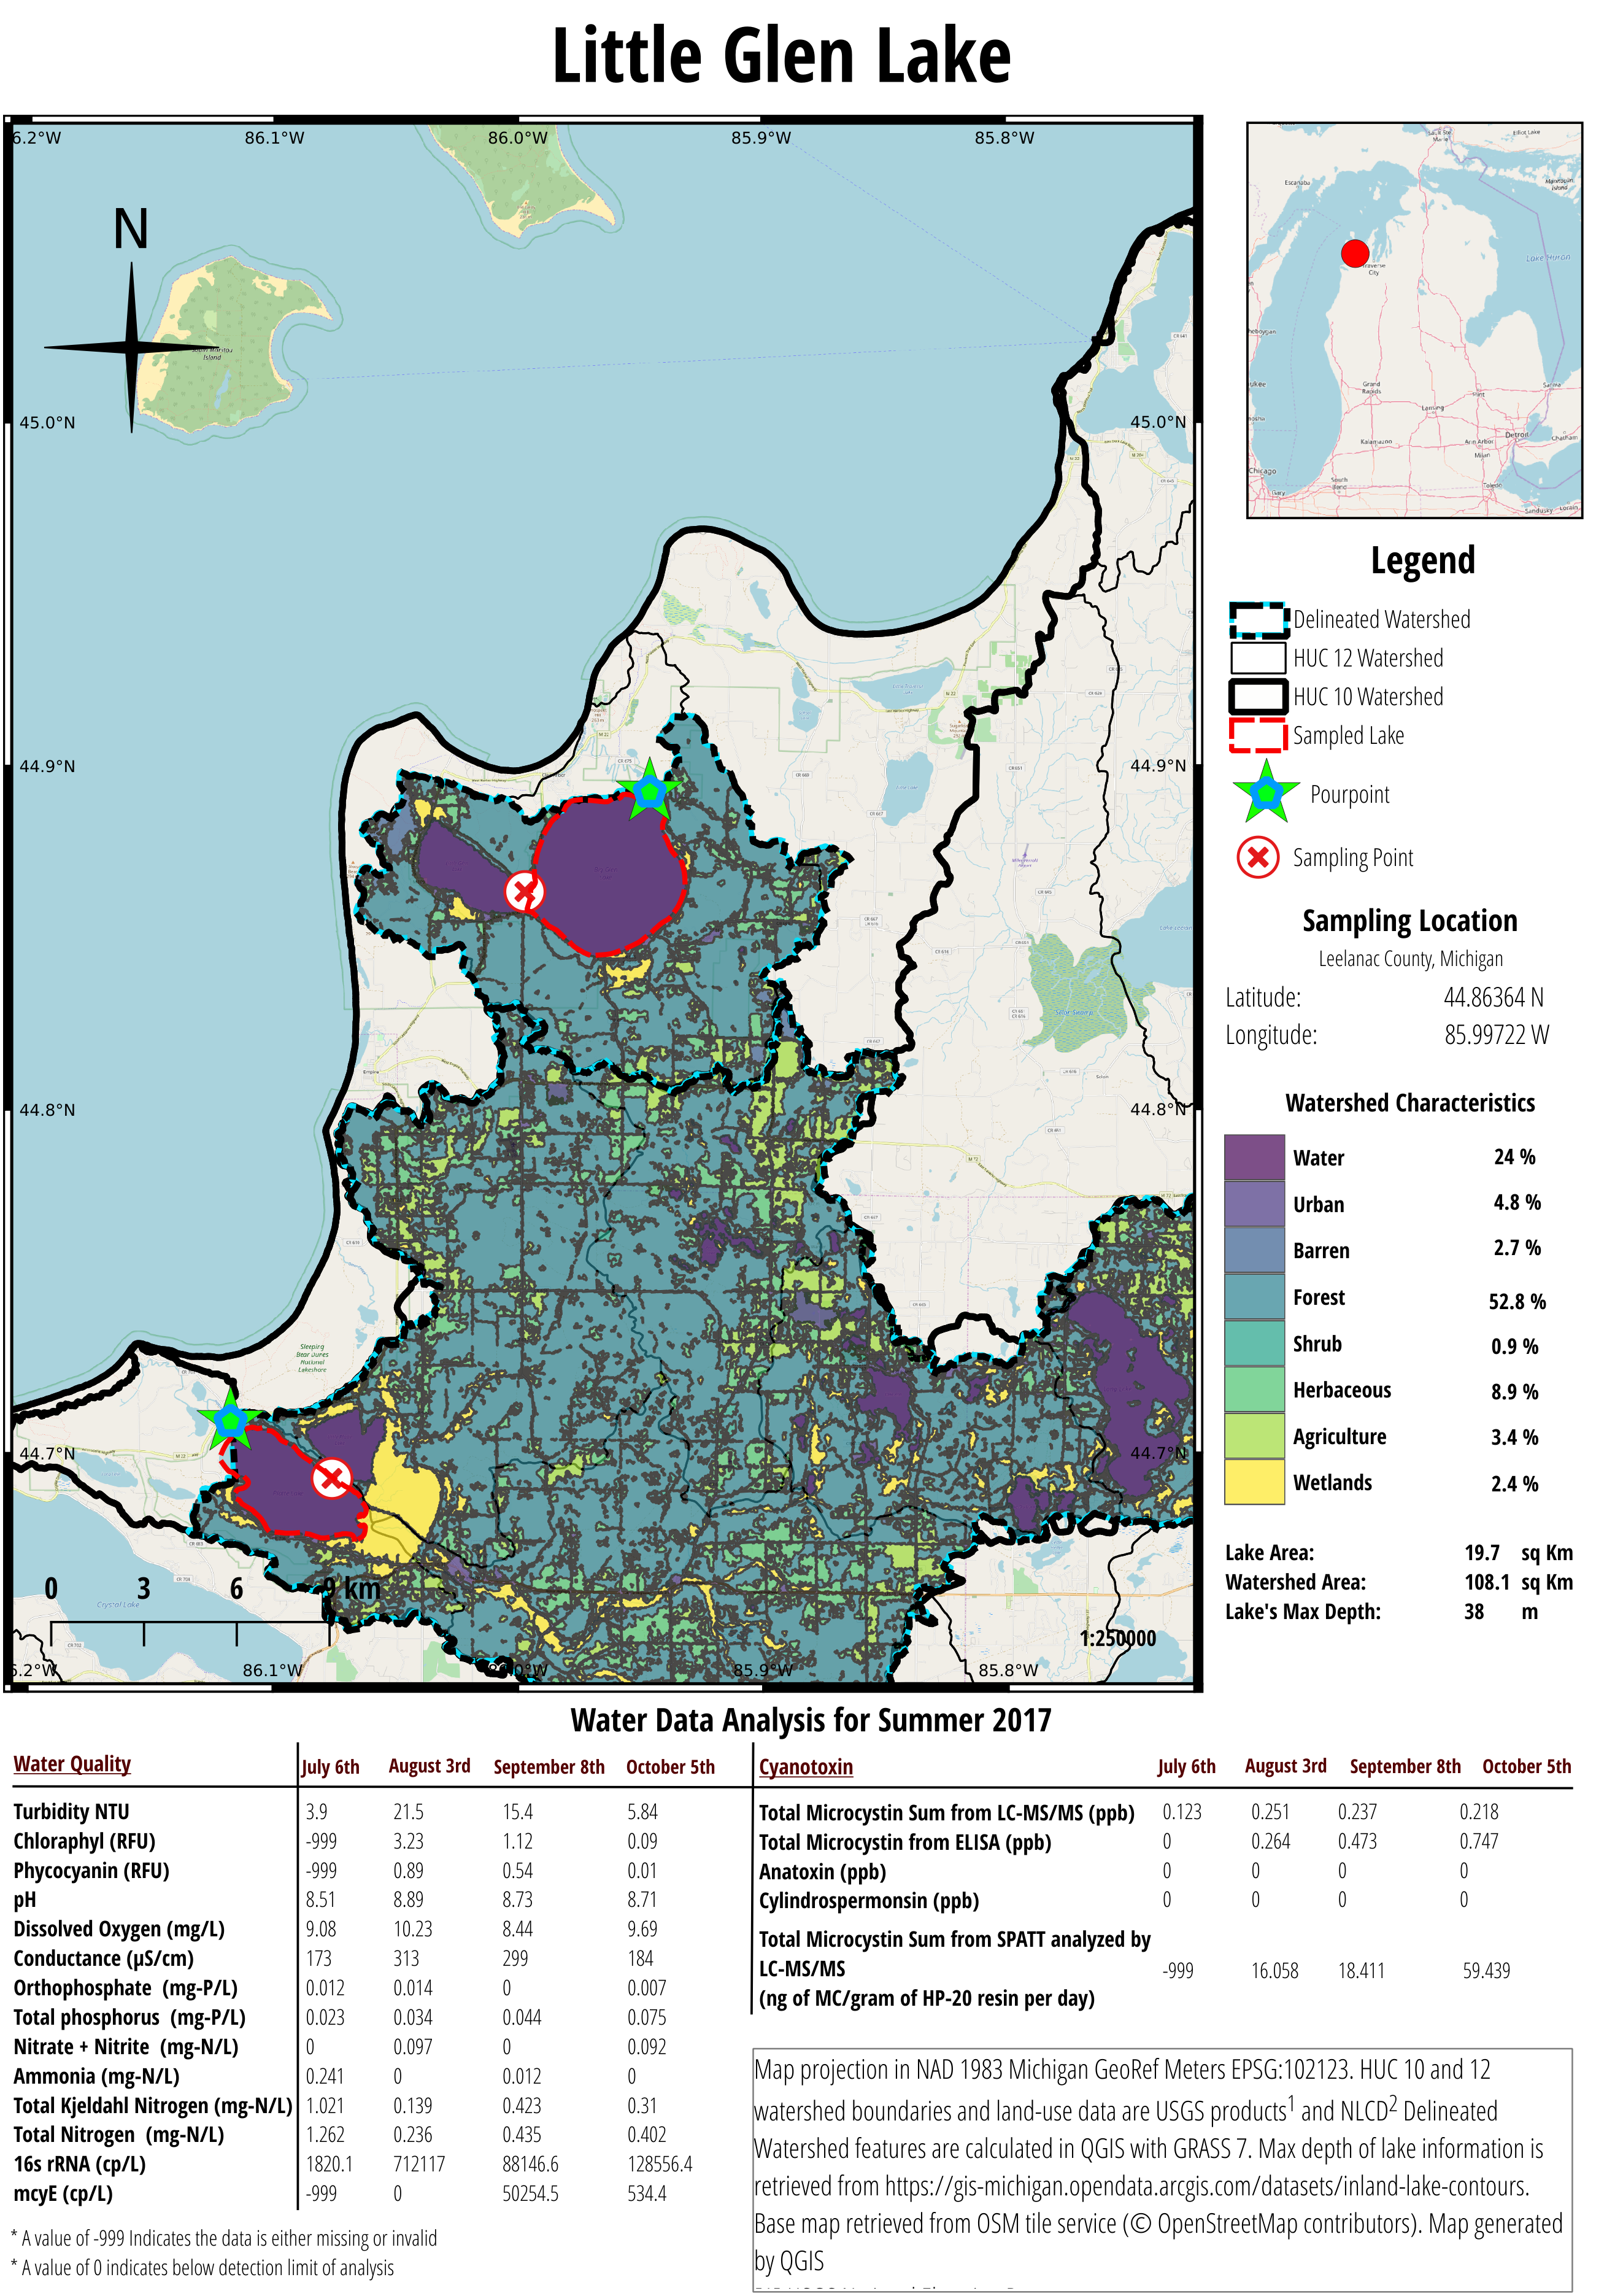
\includegraphics{figures/atlas/output_12}}
  }
\caption{GIS Map of Little Glen Lake}
\end{figure}

\begin{figure}[t]
\centerline{%
  \resizebox{\textwidth}{!}{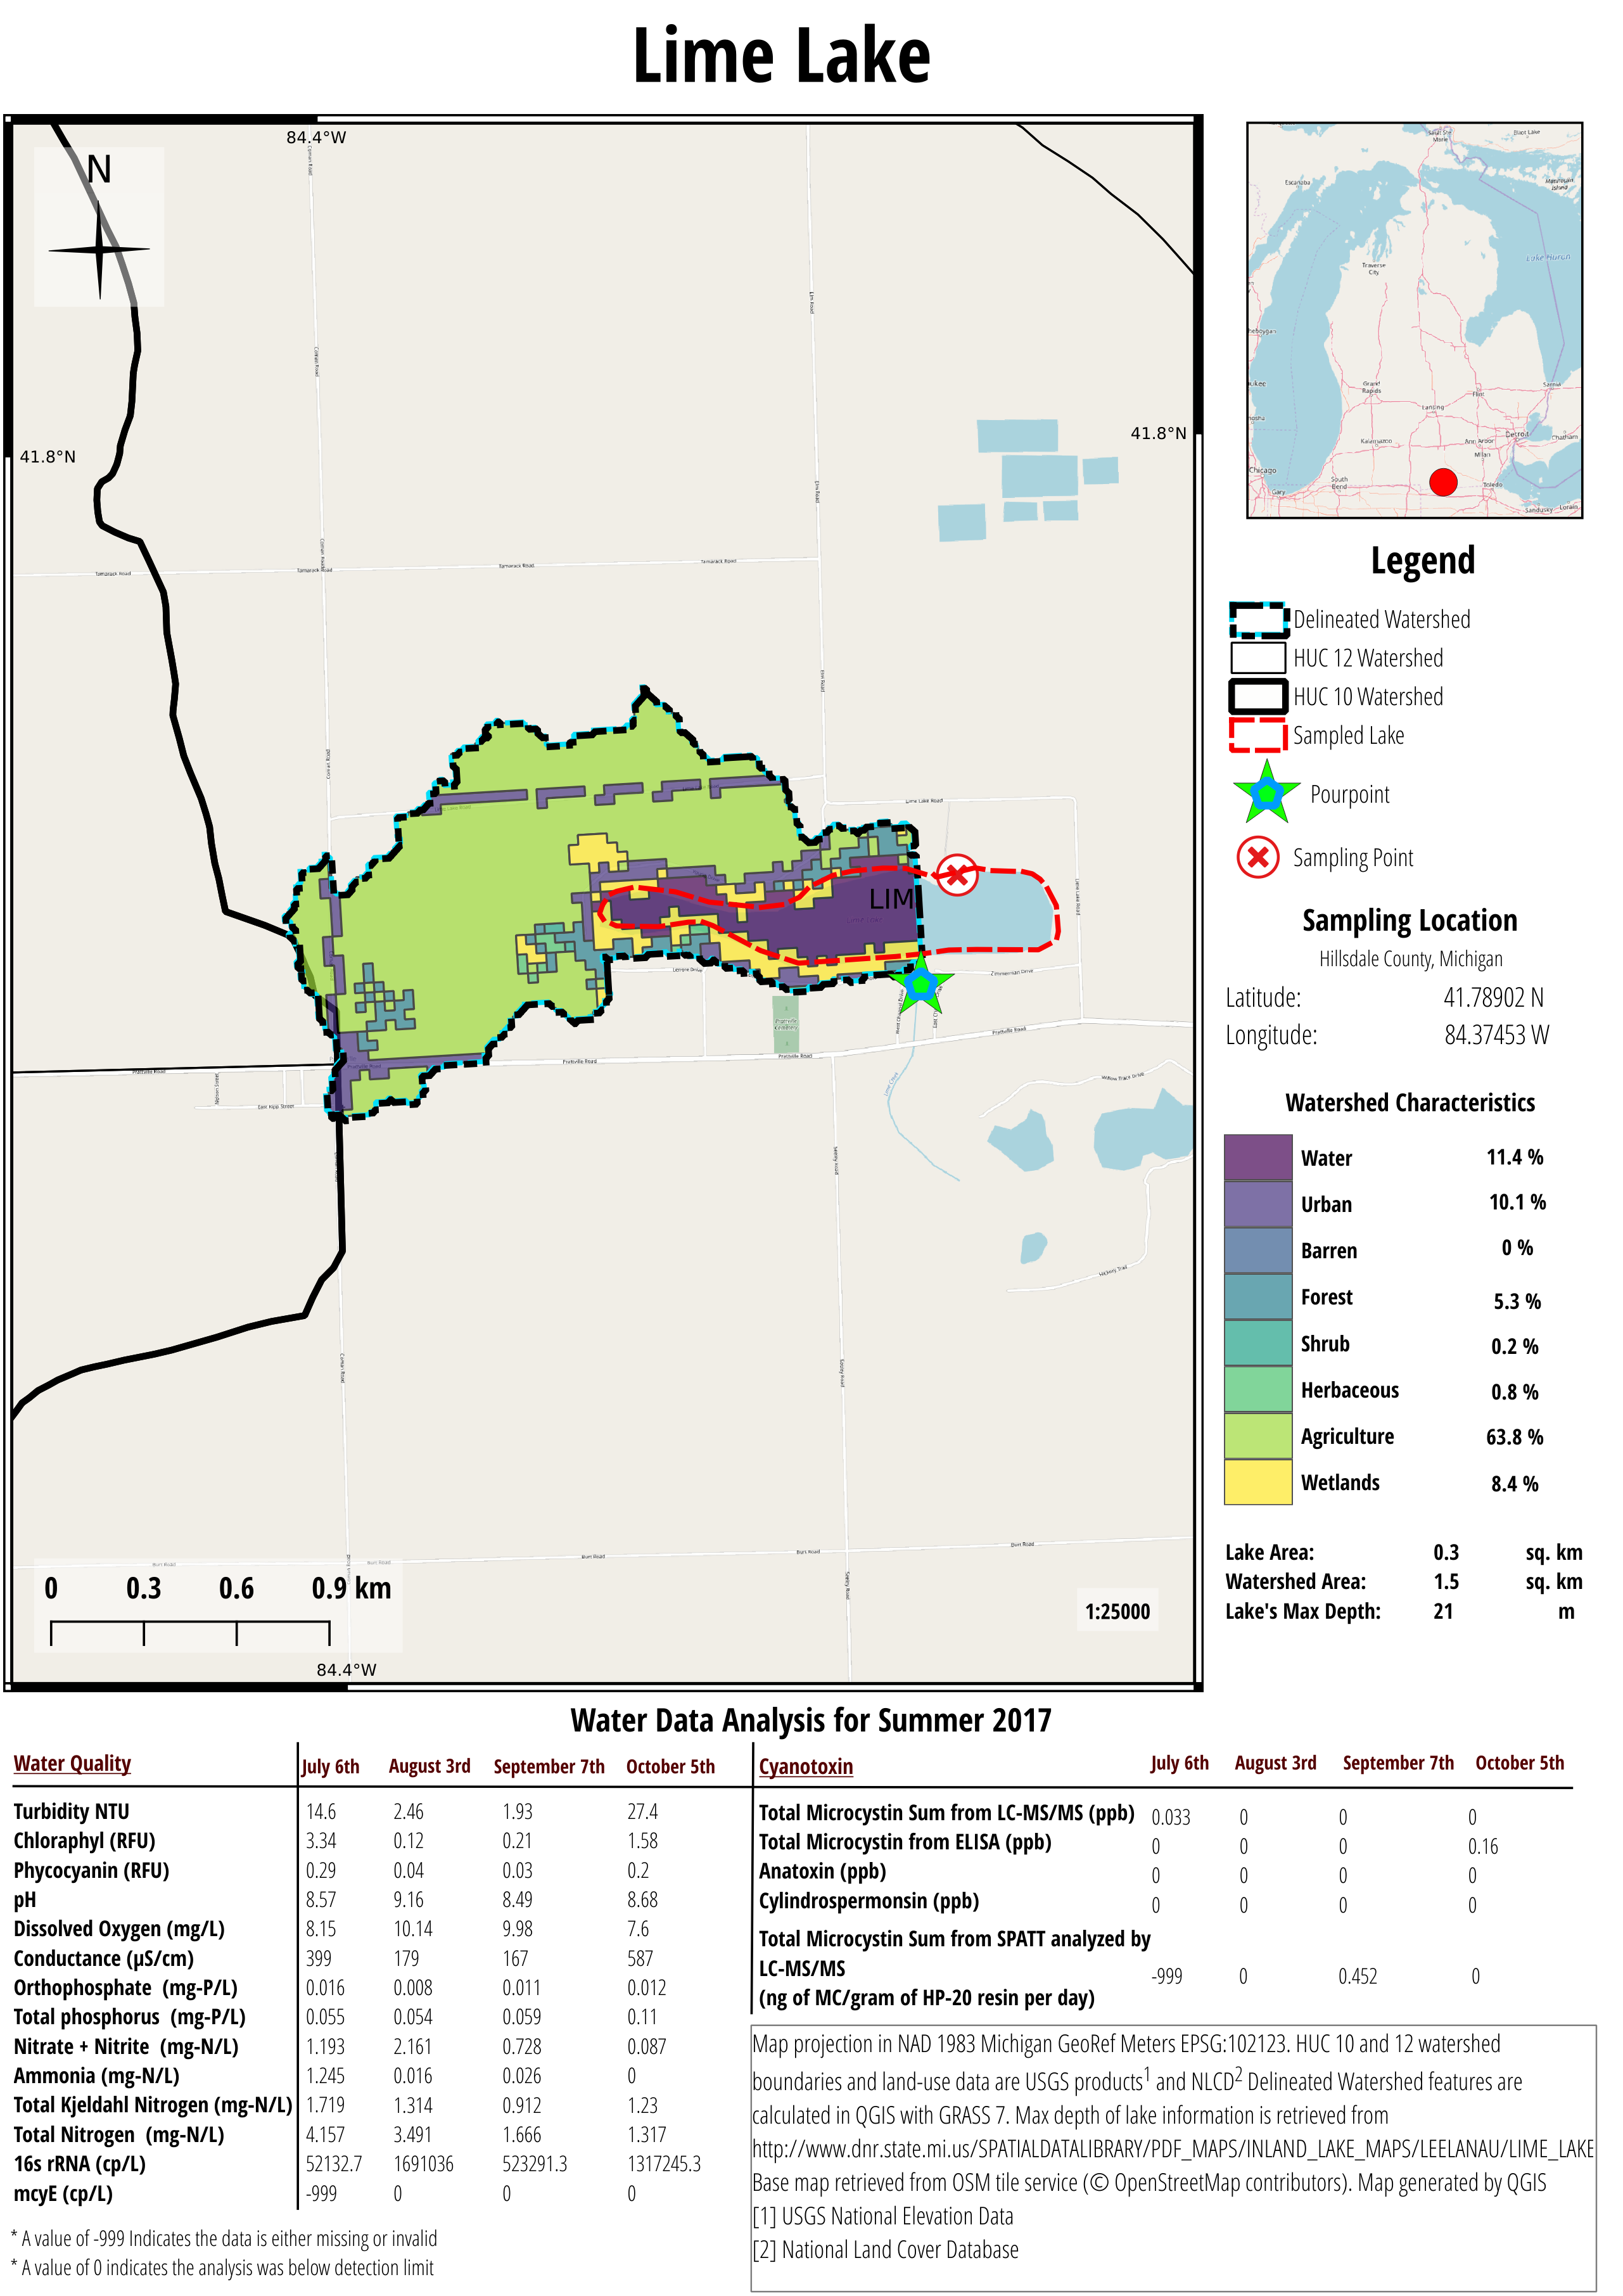
\includegraphics{figures/atlas/output_13}}
  }
\caption{GIS Map of Lime Lake}
\end{figure}

\begin{figure}[t]
\centerline{%
  \resizebox{\textwidth}{!}{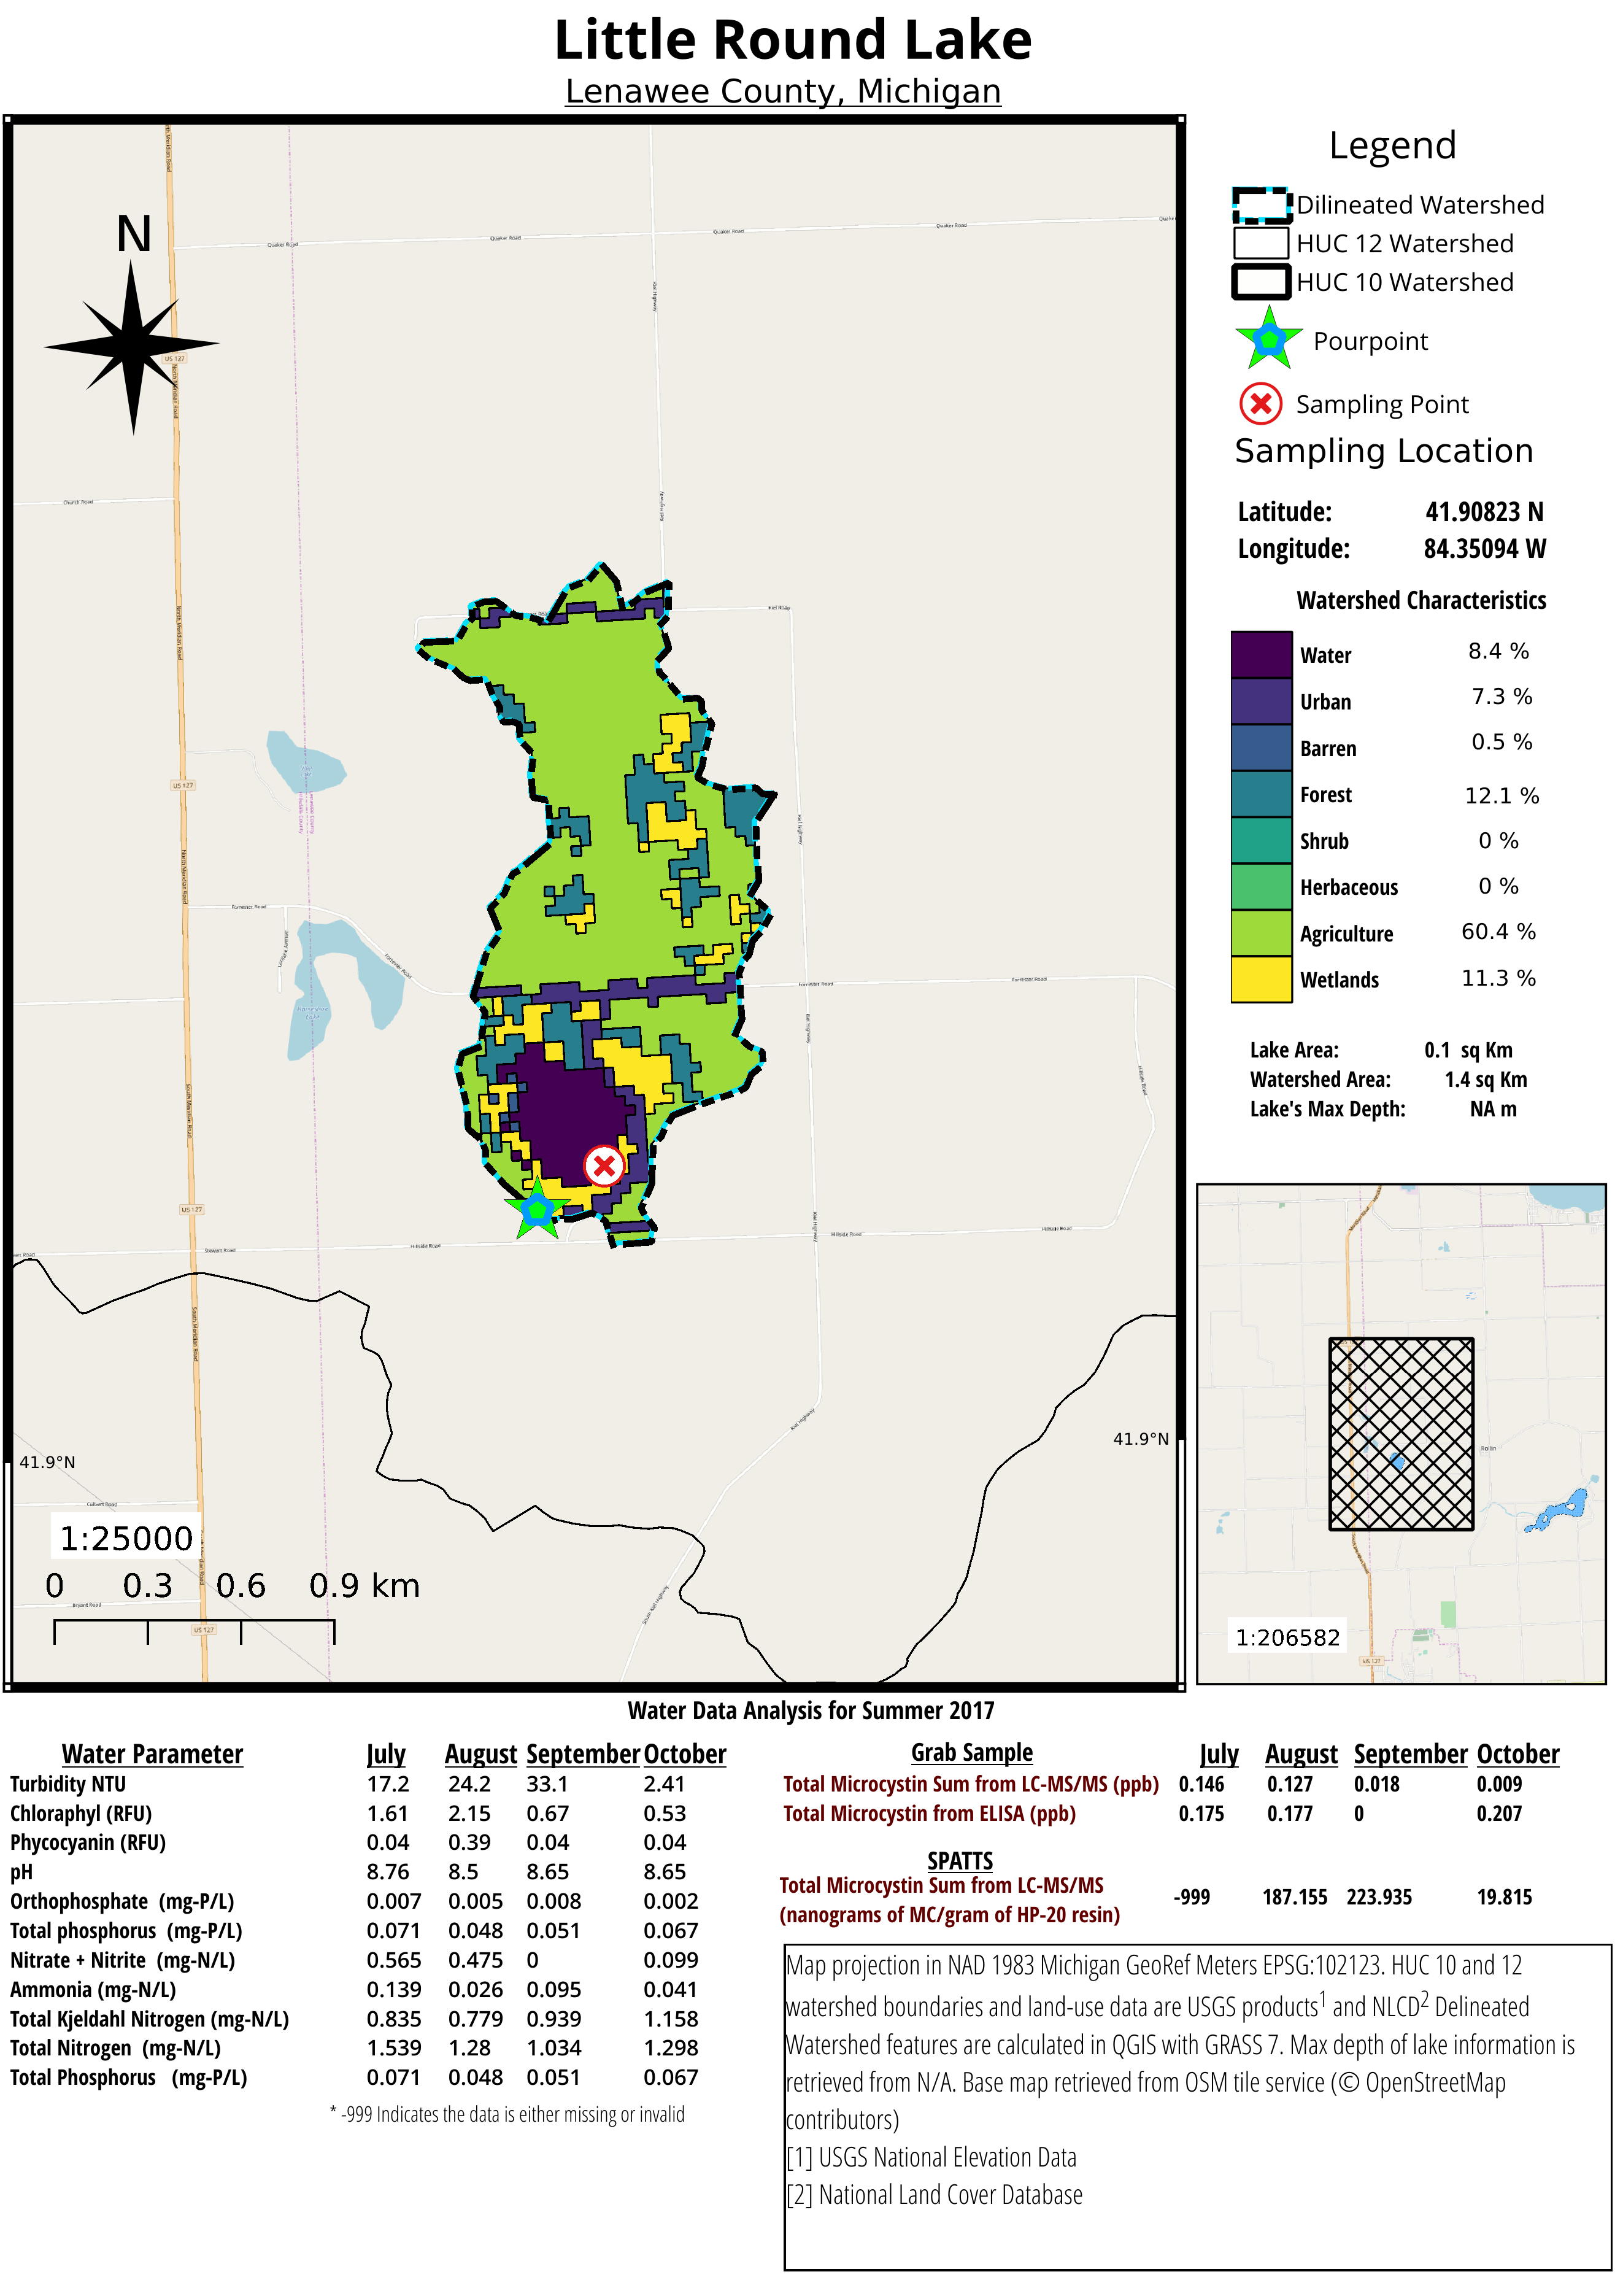
\includegraphics{figures/atlas/output_14}}
  }
\caption{GIS Map of Little Round Lake}
\end{figure}

\begin{figure}[t]
\centerline{%
  \resizebox{\textwidth}{!}{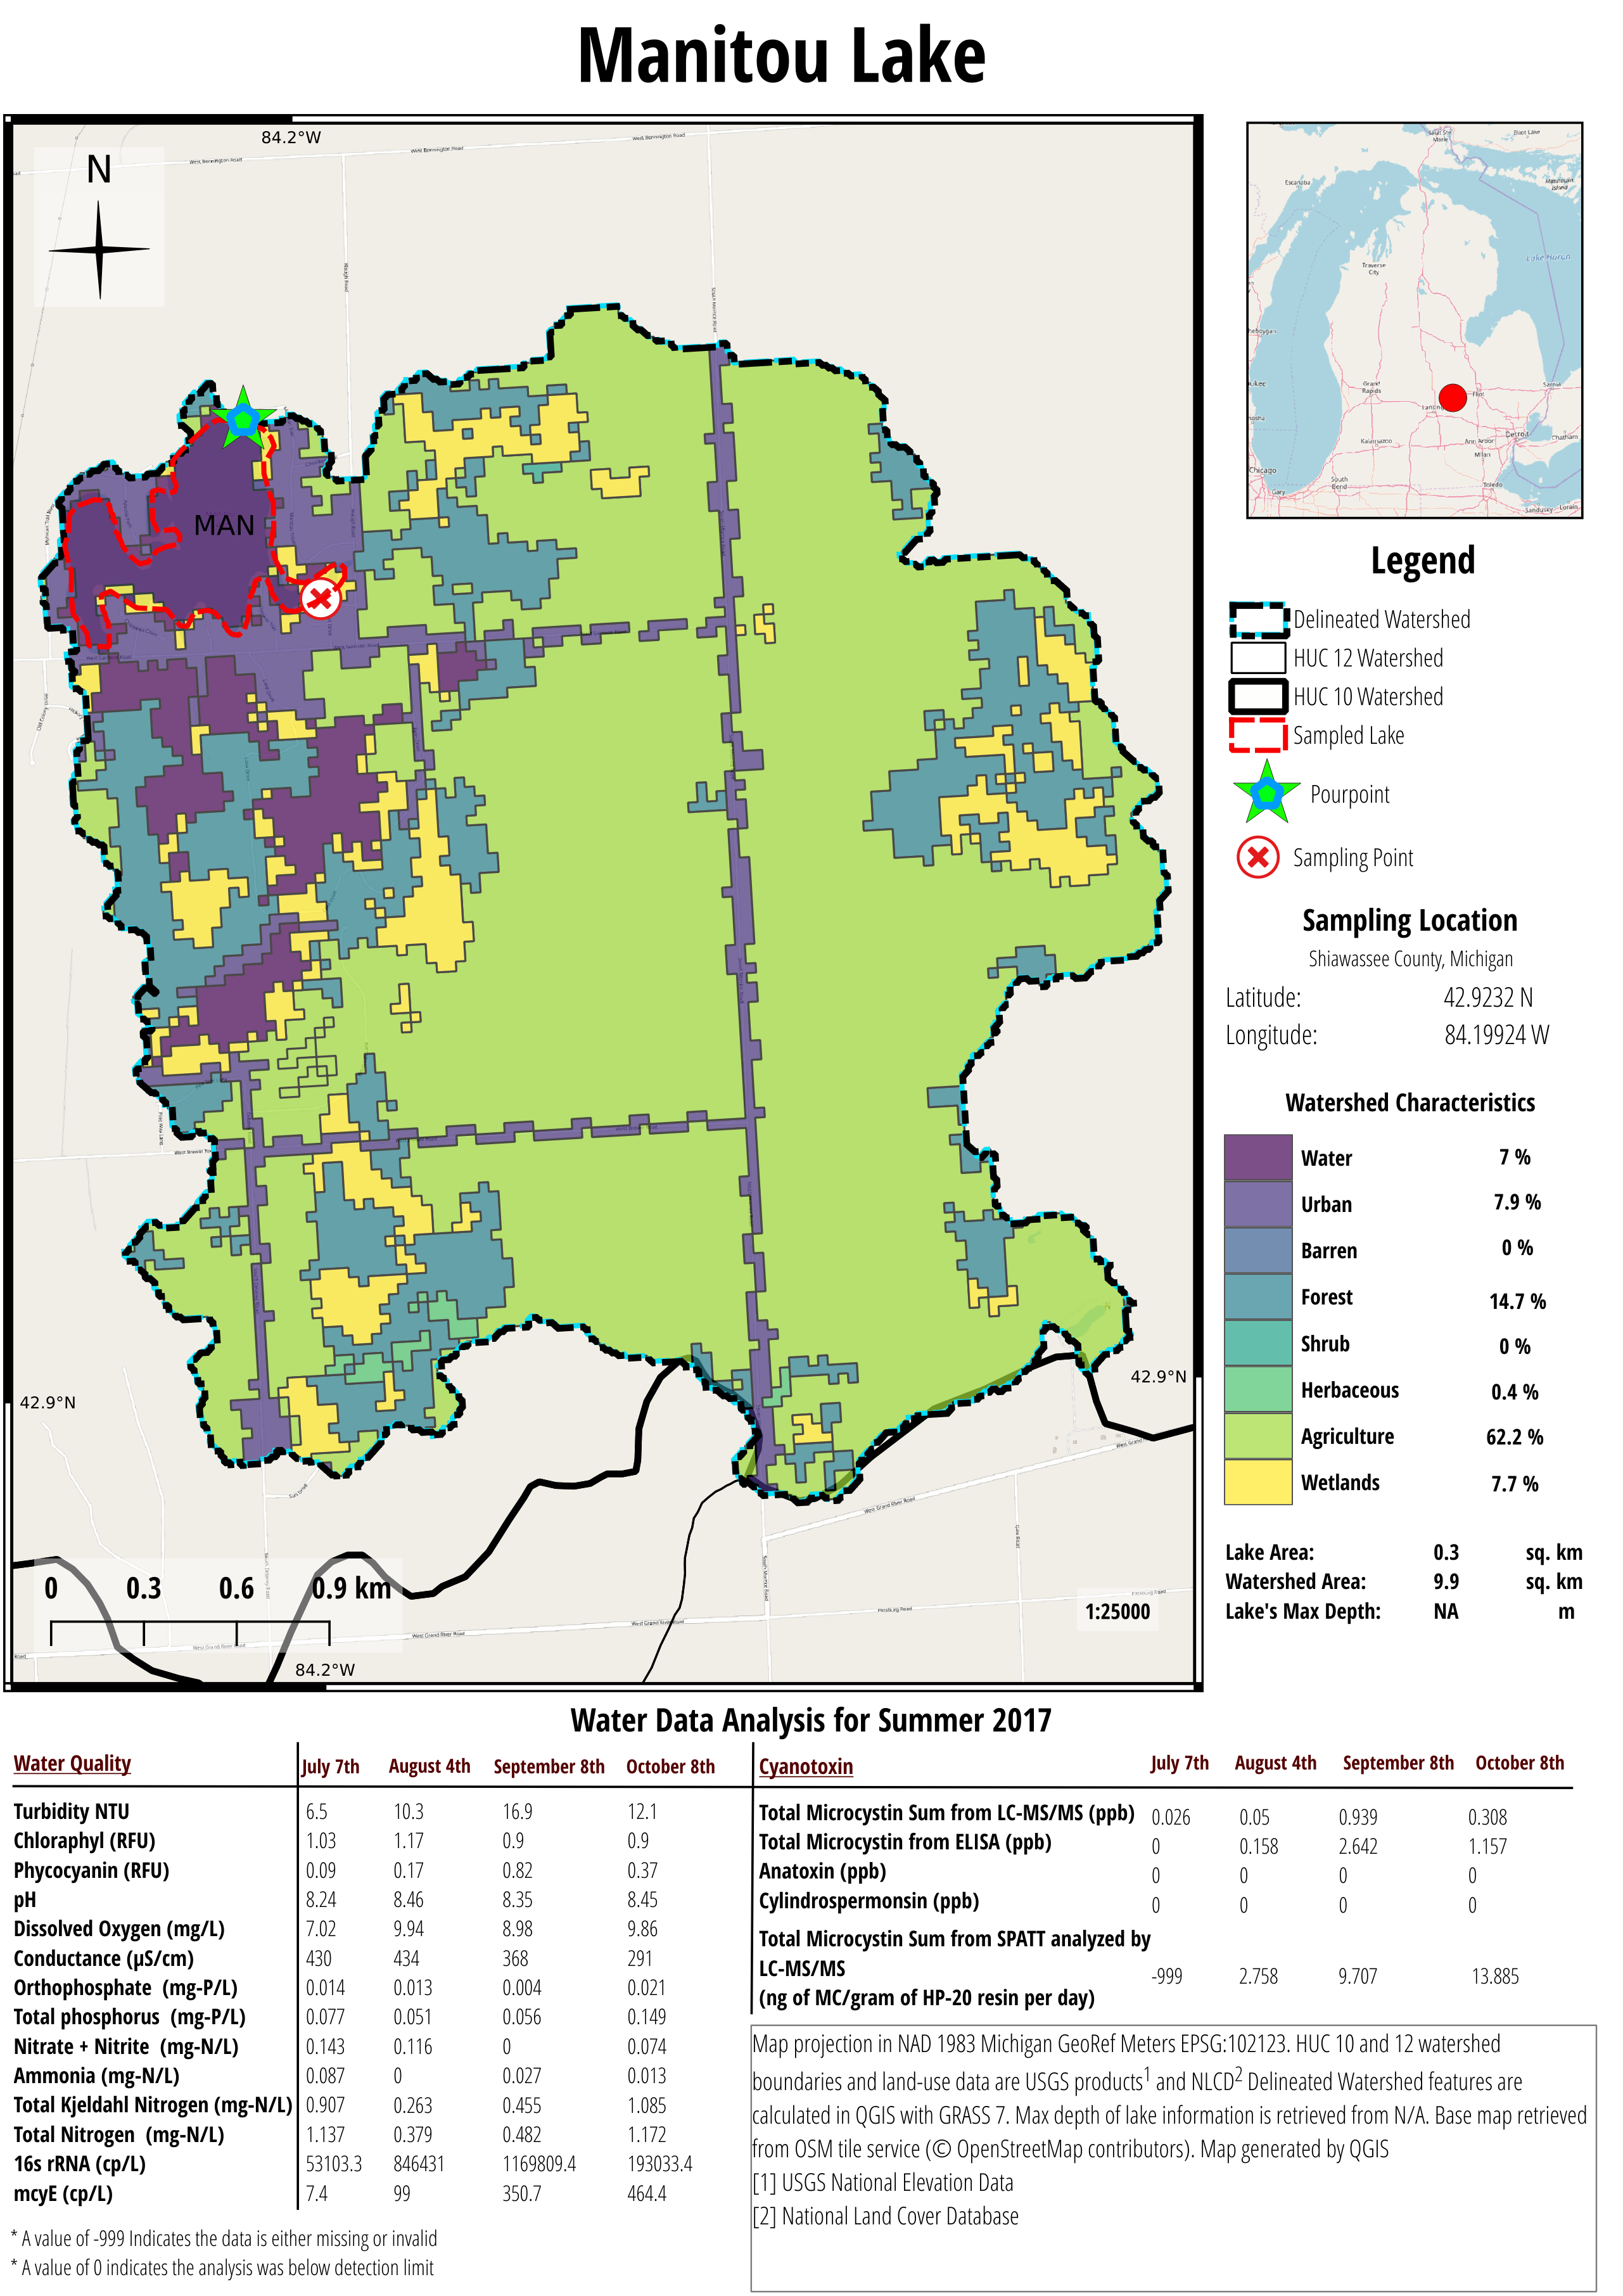
\includegraphics{figures/atlas/output_15}}
  }
\caption{GIS Map of Manitou Lake}
\end{figure}

\begin{figure}[t]
\centerline{%
  \resizebox{\textwidth}{!}{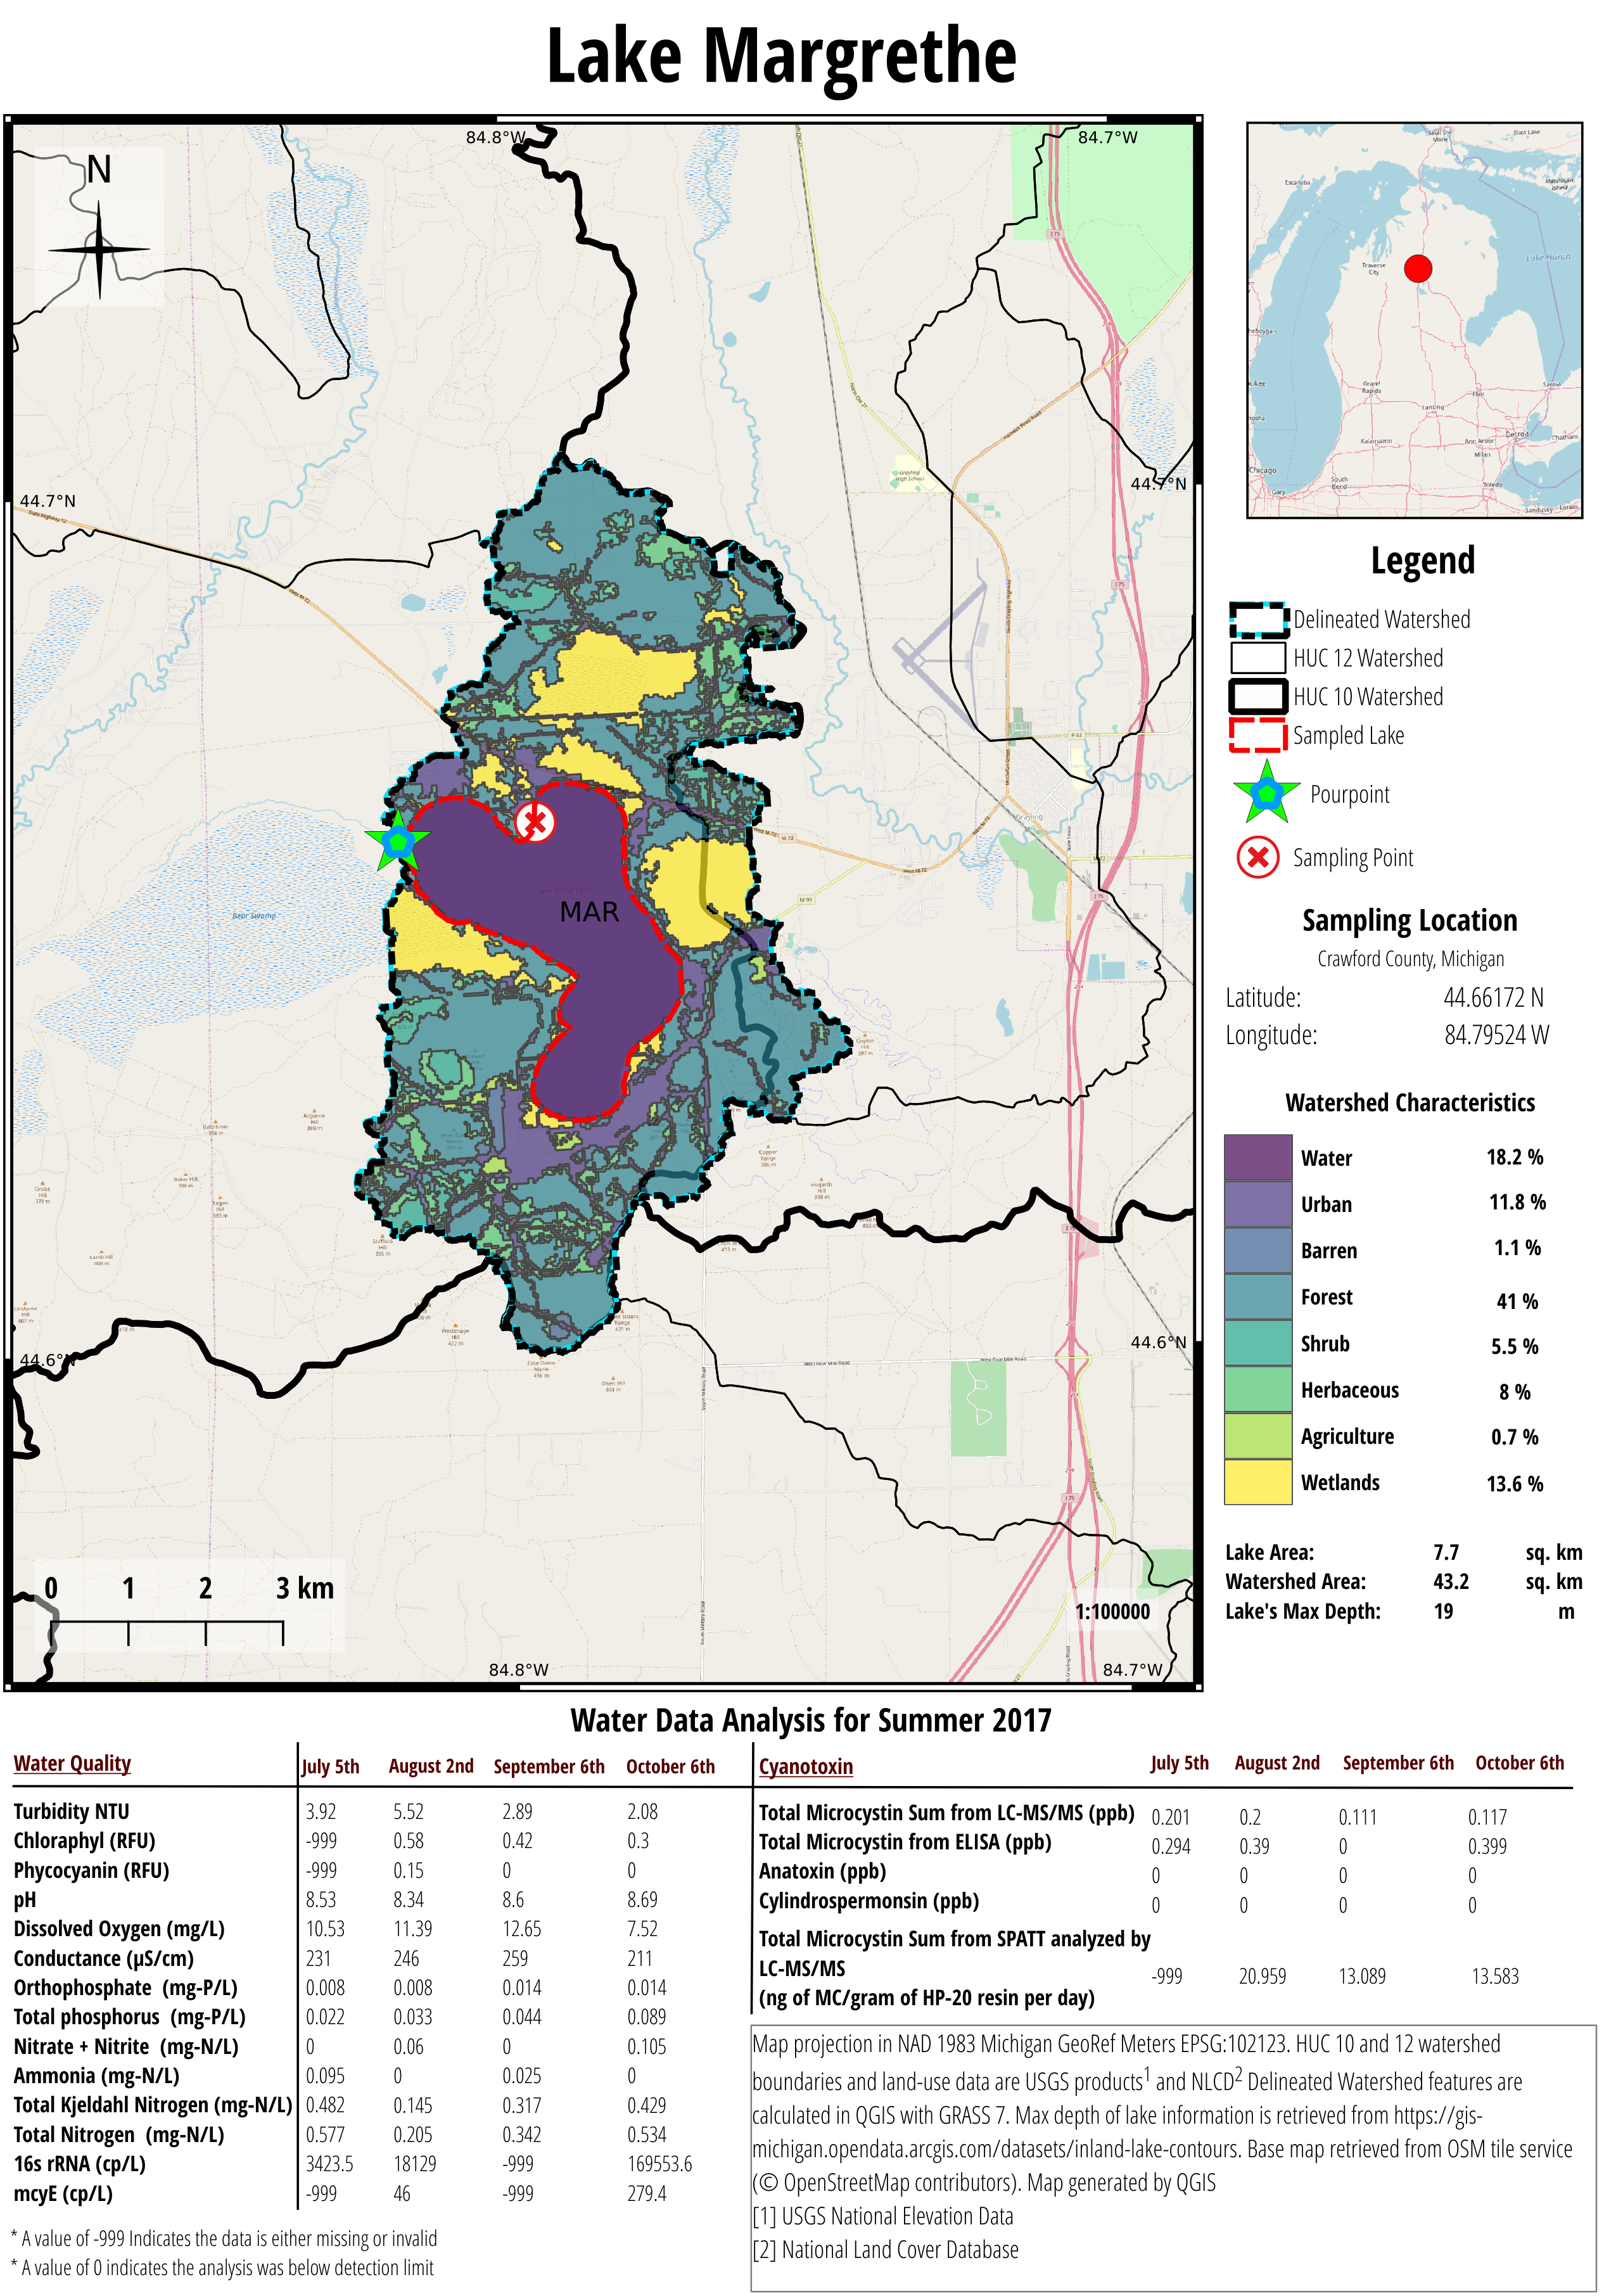
\includegraphics{figures/atlas/output_16}}
  }
\caption{GIS Map of Lake Margrethe}
\end{figure}

\begin{figure}[t]
\centerline{%
  \resizebox{\textwidth}{!}{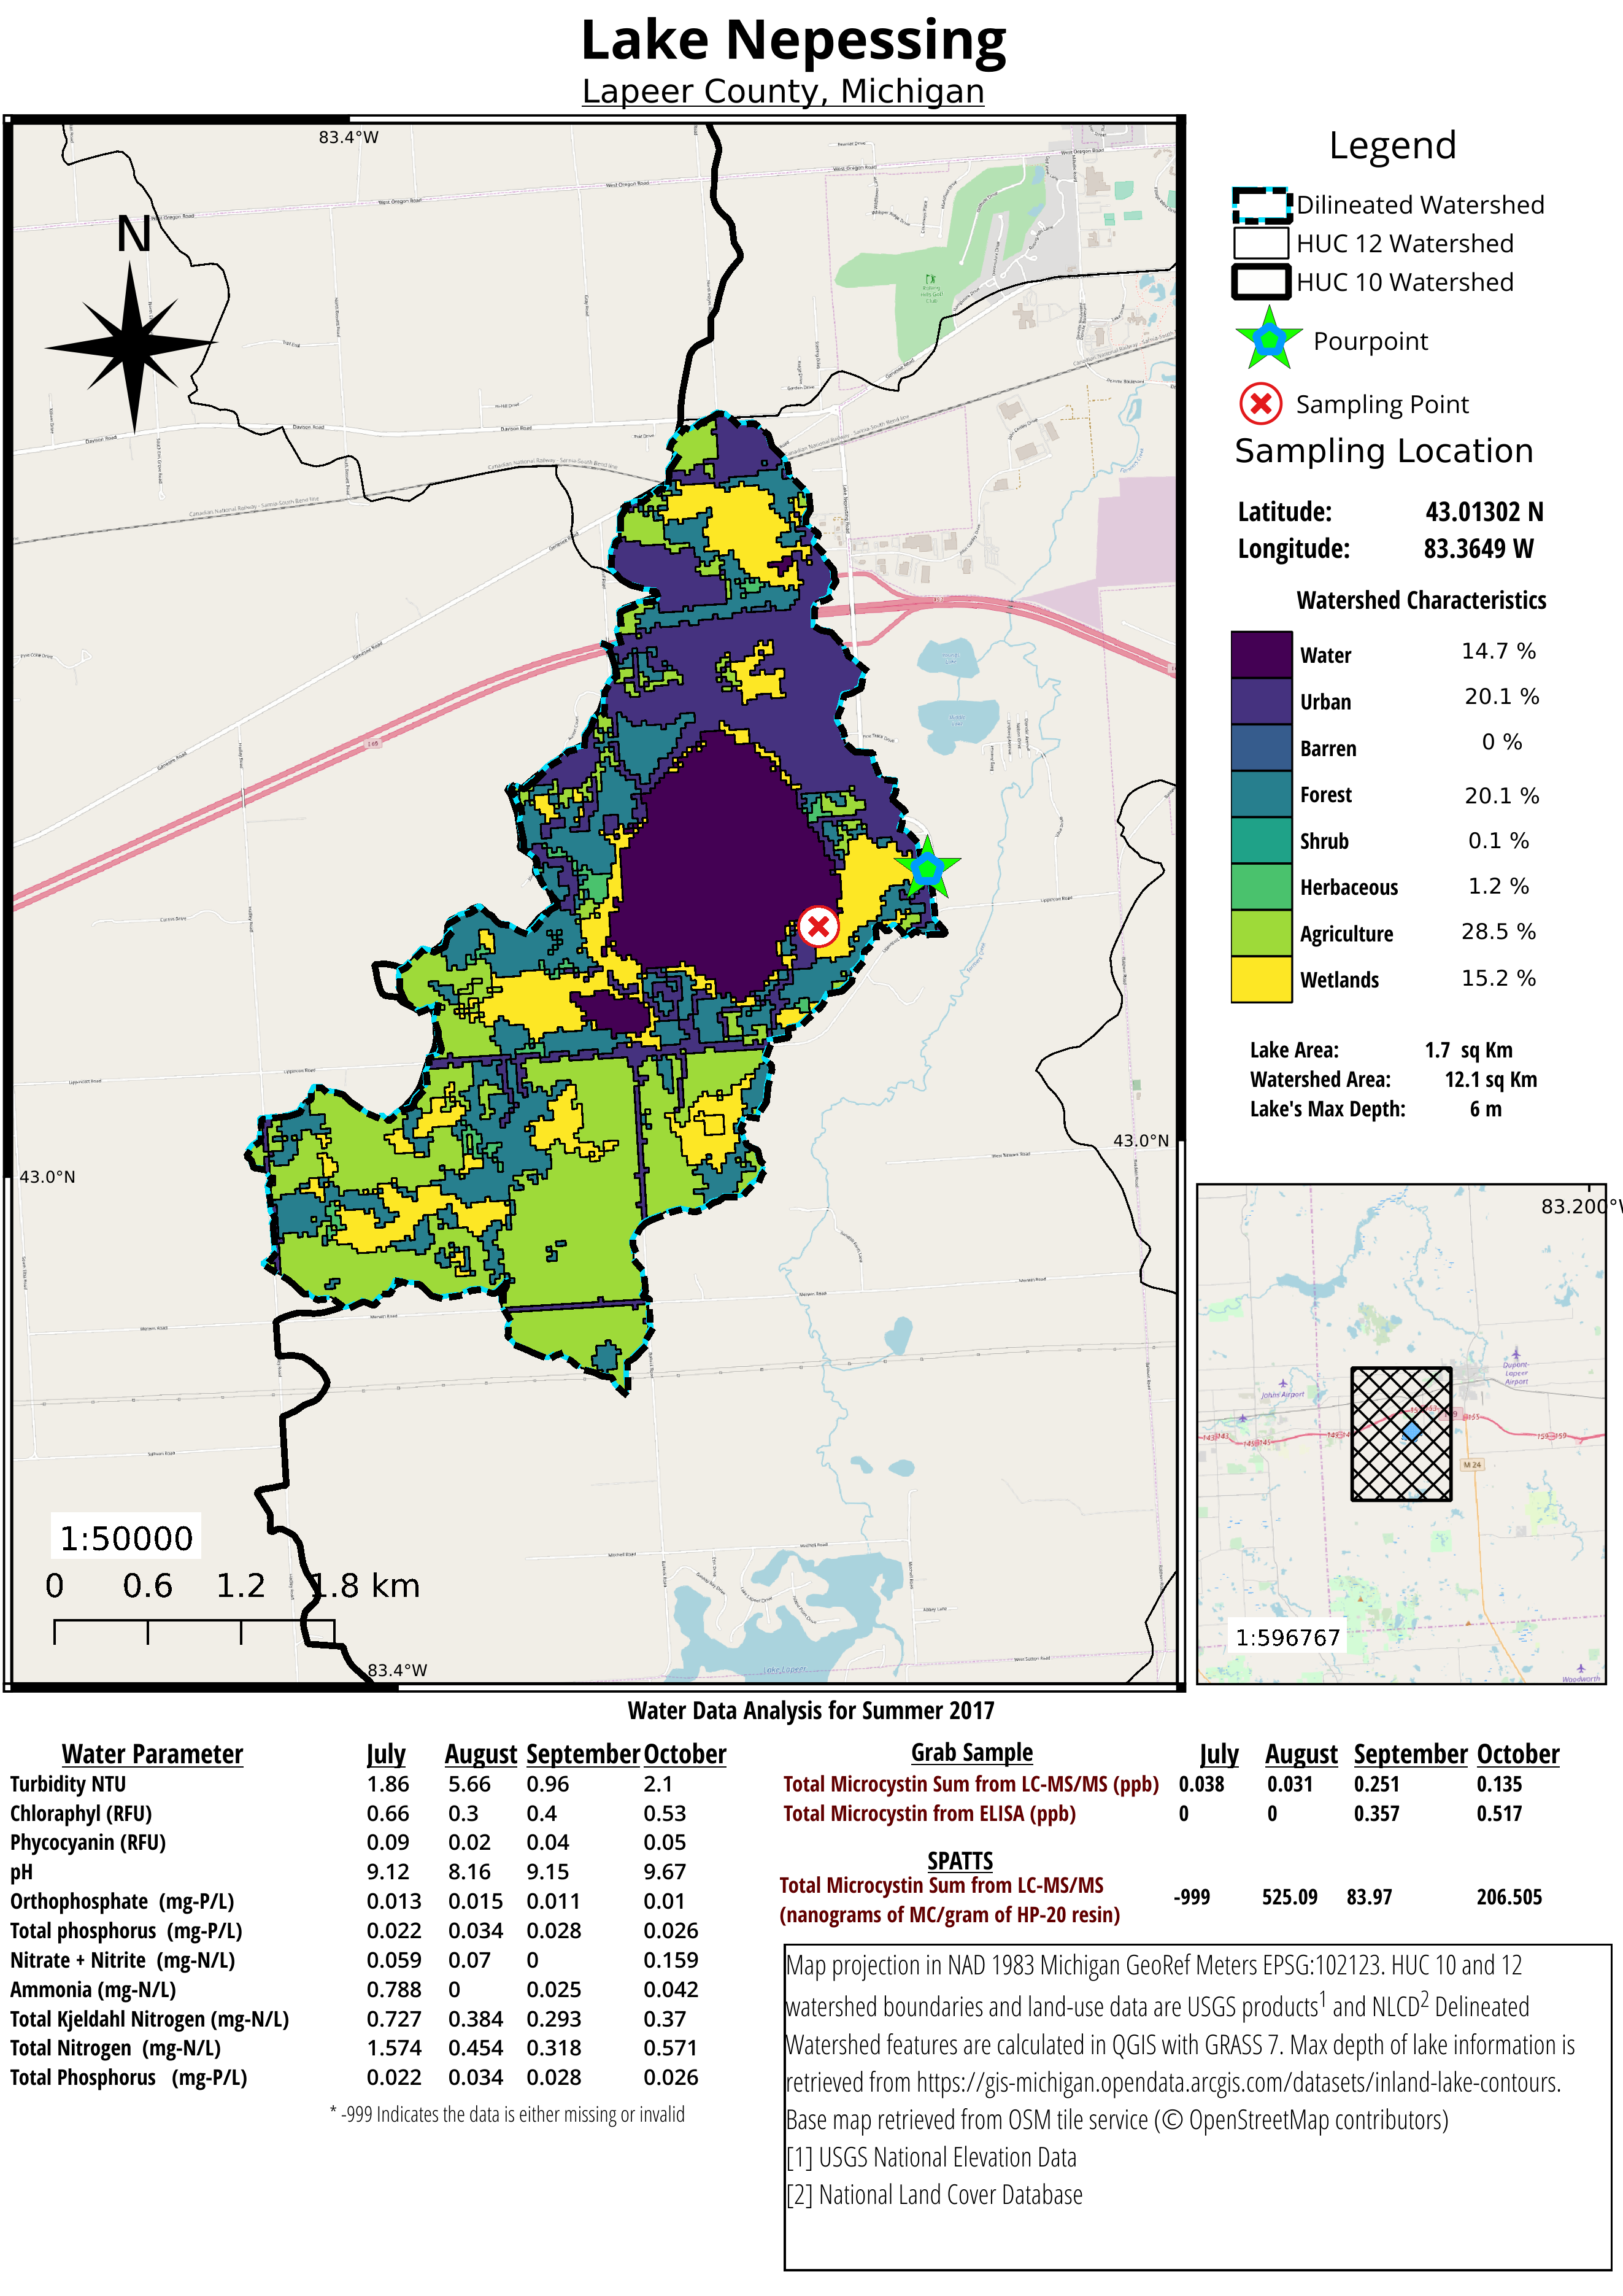
\includegraphics{figures/atlas/output_17}}
  }
\caption{GIS Map of Lake Nepessing}
\end{figure}

\begin{figure}[t]
\centerline{%
  \resizebox{\textwidth}{!}{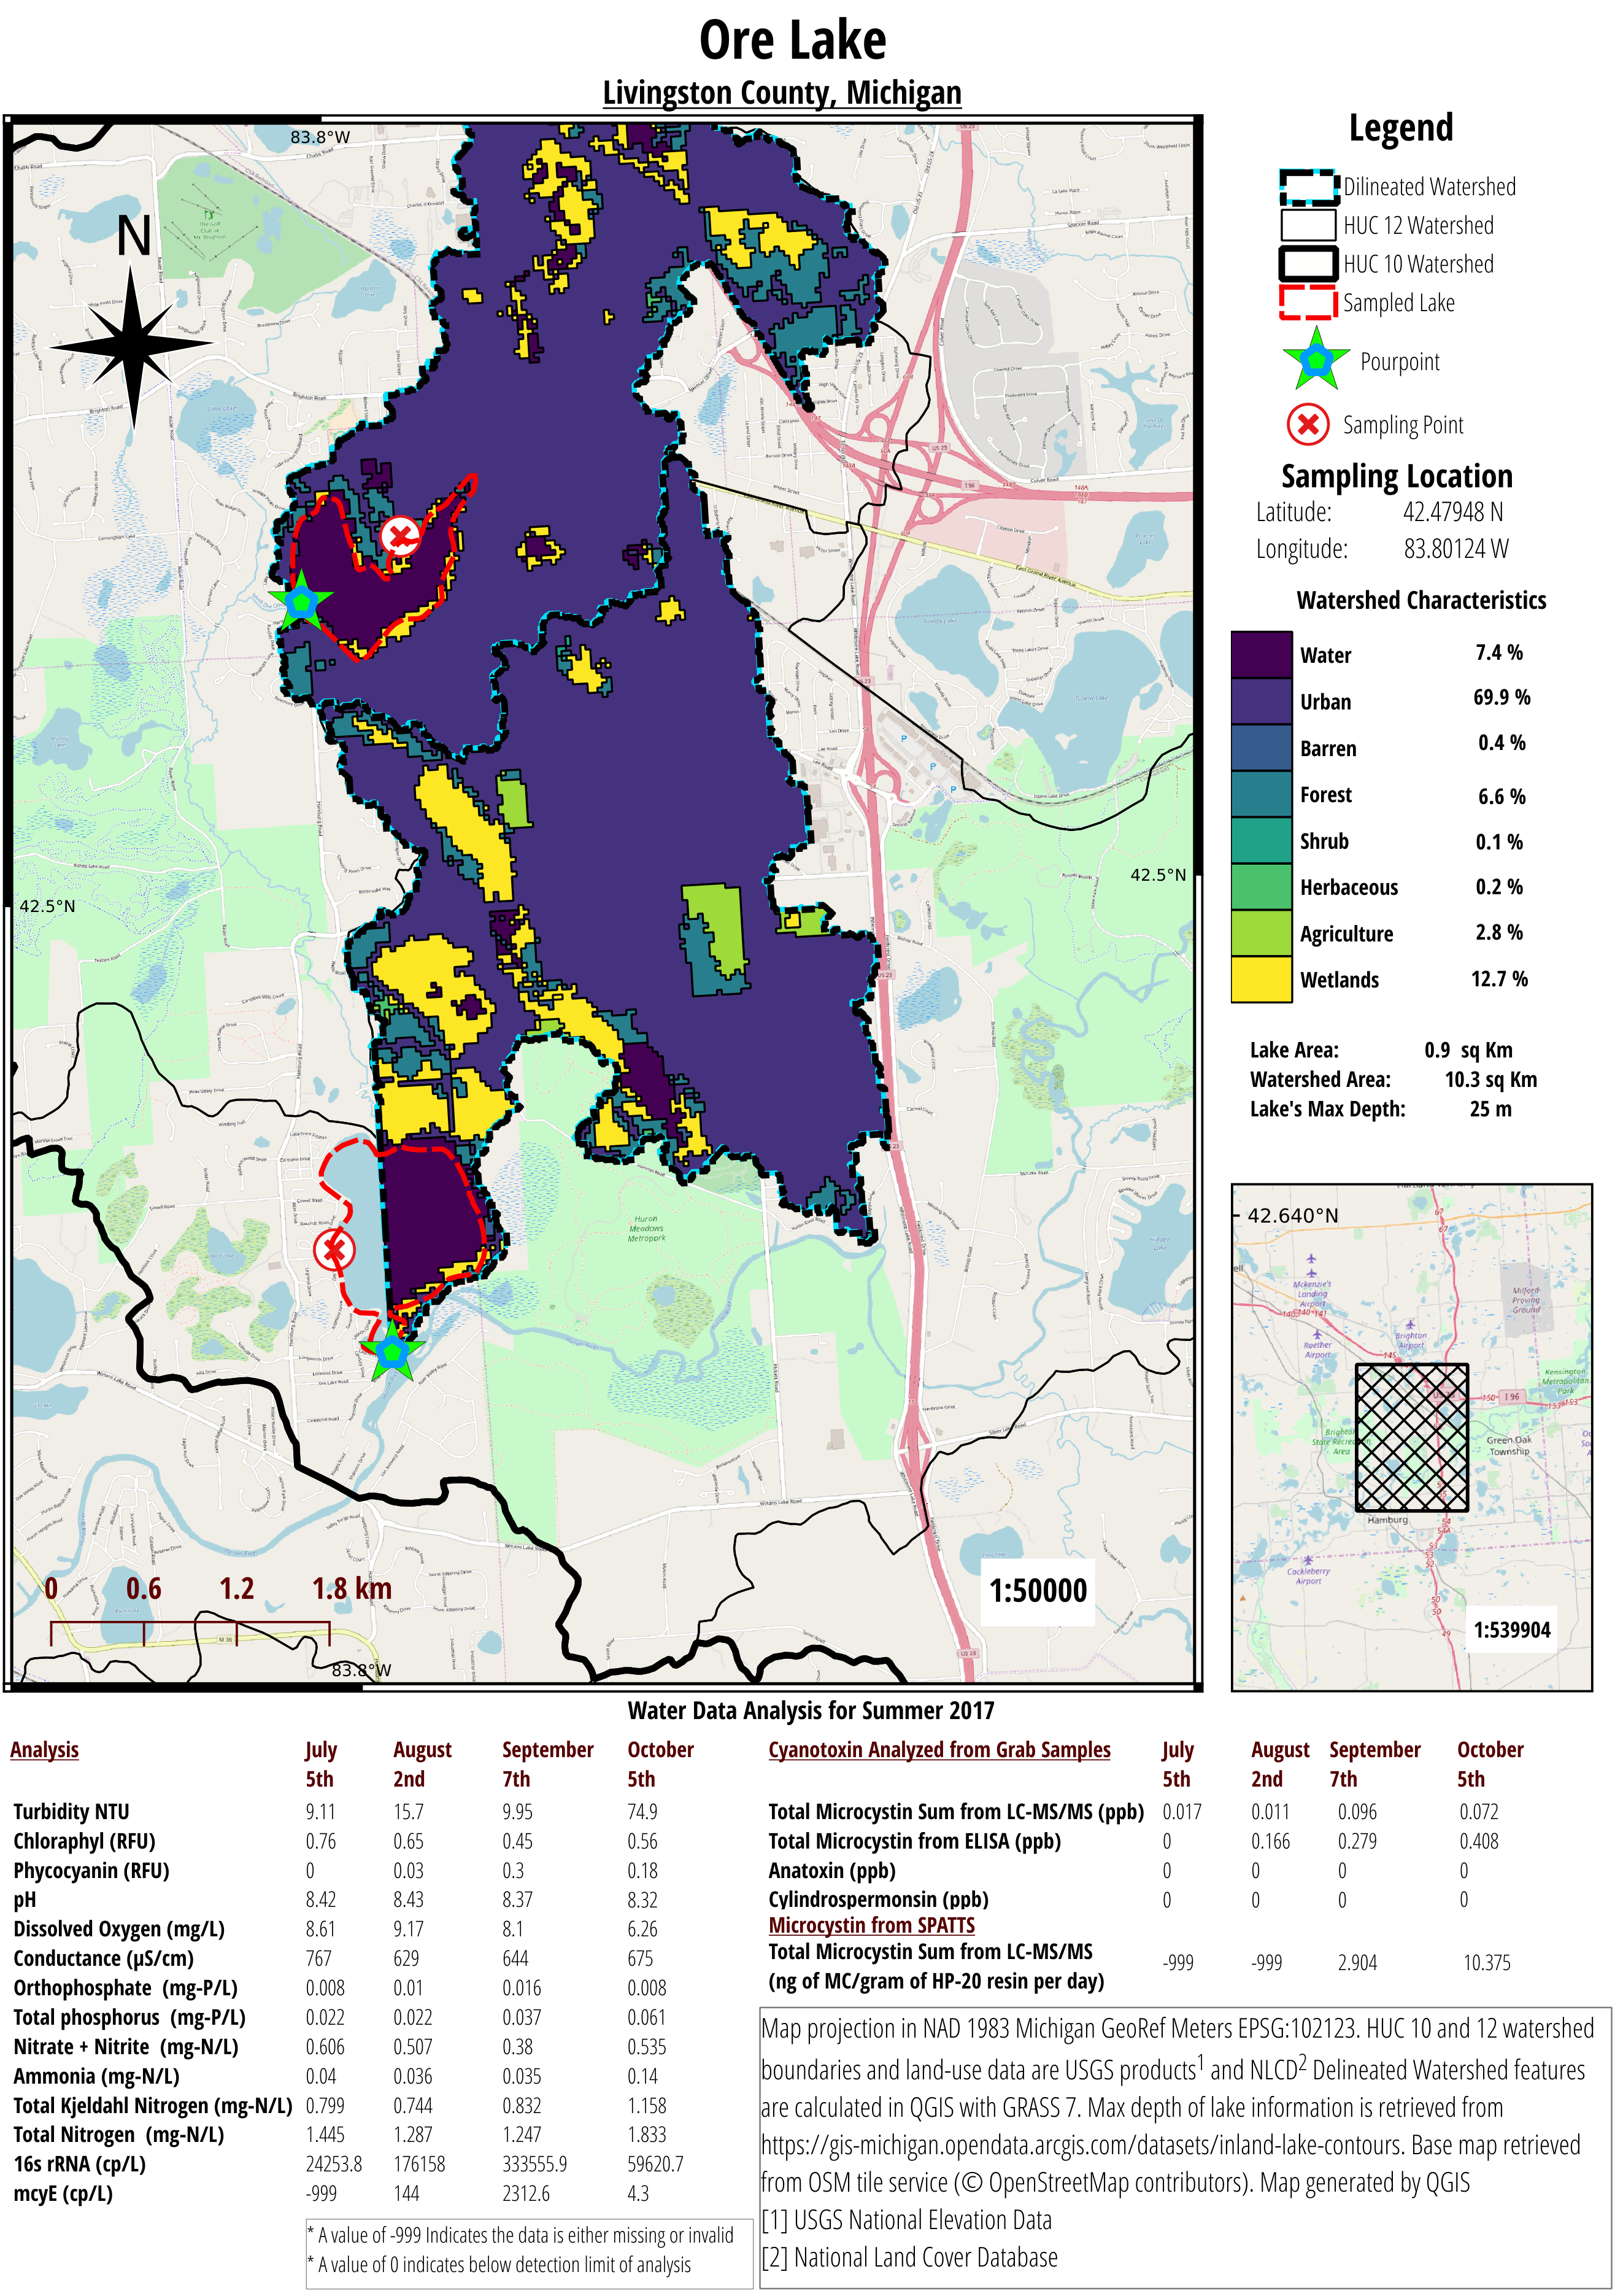
\includegraphics{figures/atlas/output_18}}
  }
\caption{GIS Map of Ore Lake}
\end{figure}

\begin{figure}[t]
\centerline{%
  \resizebox{\textwidth}{!}{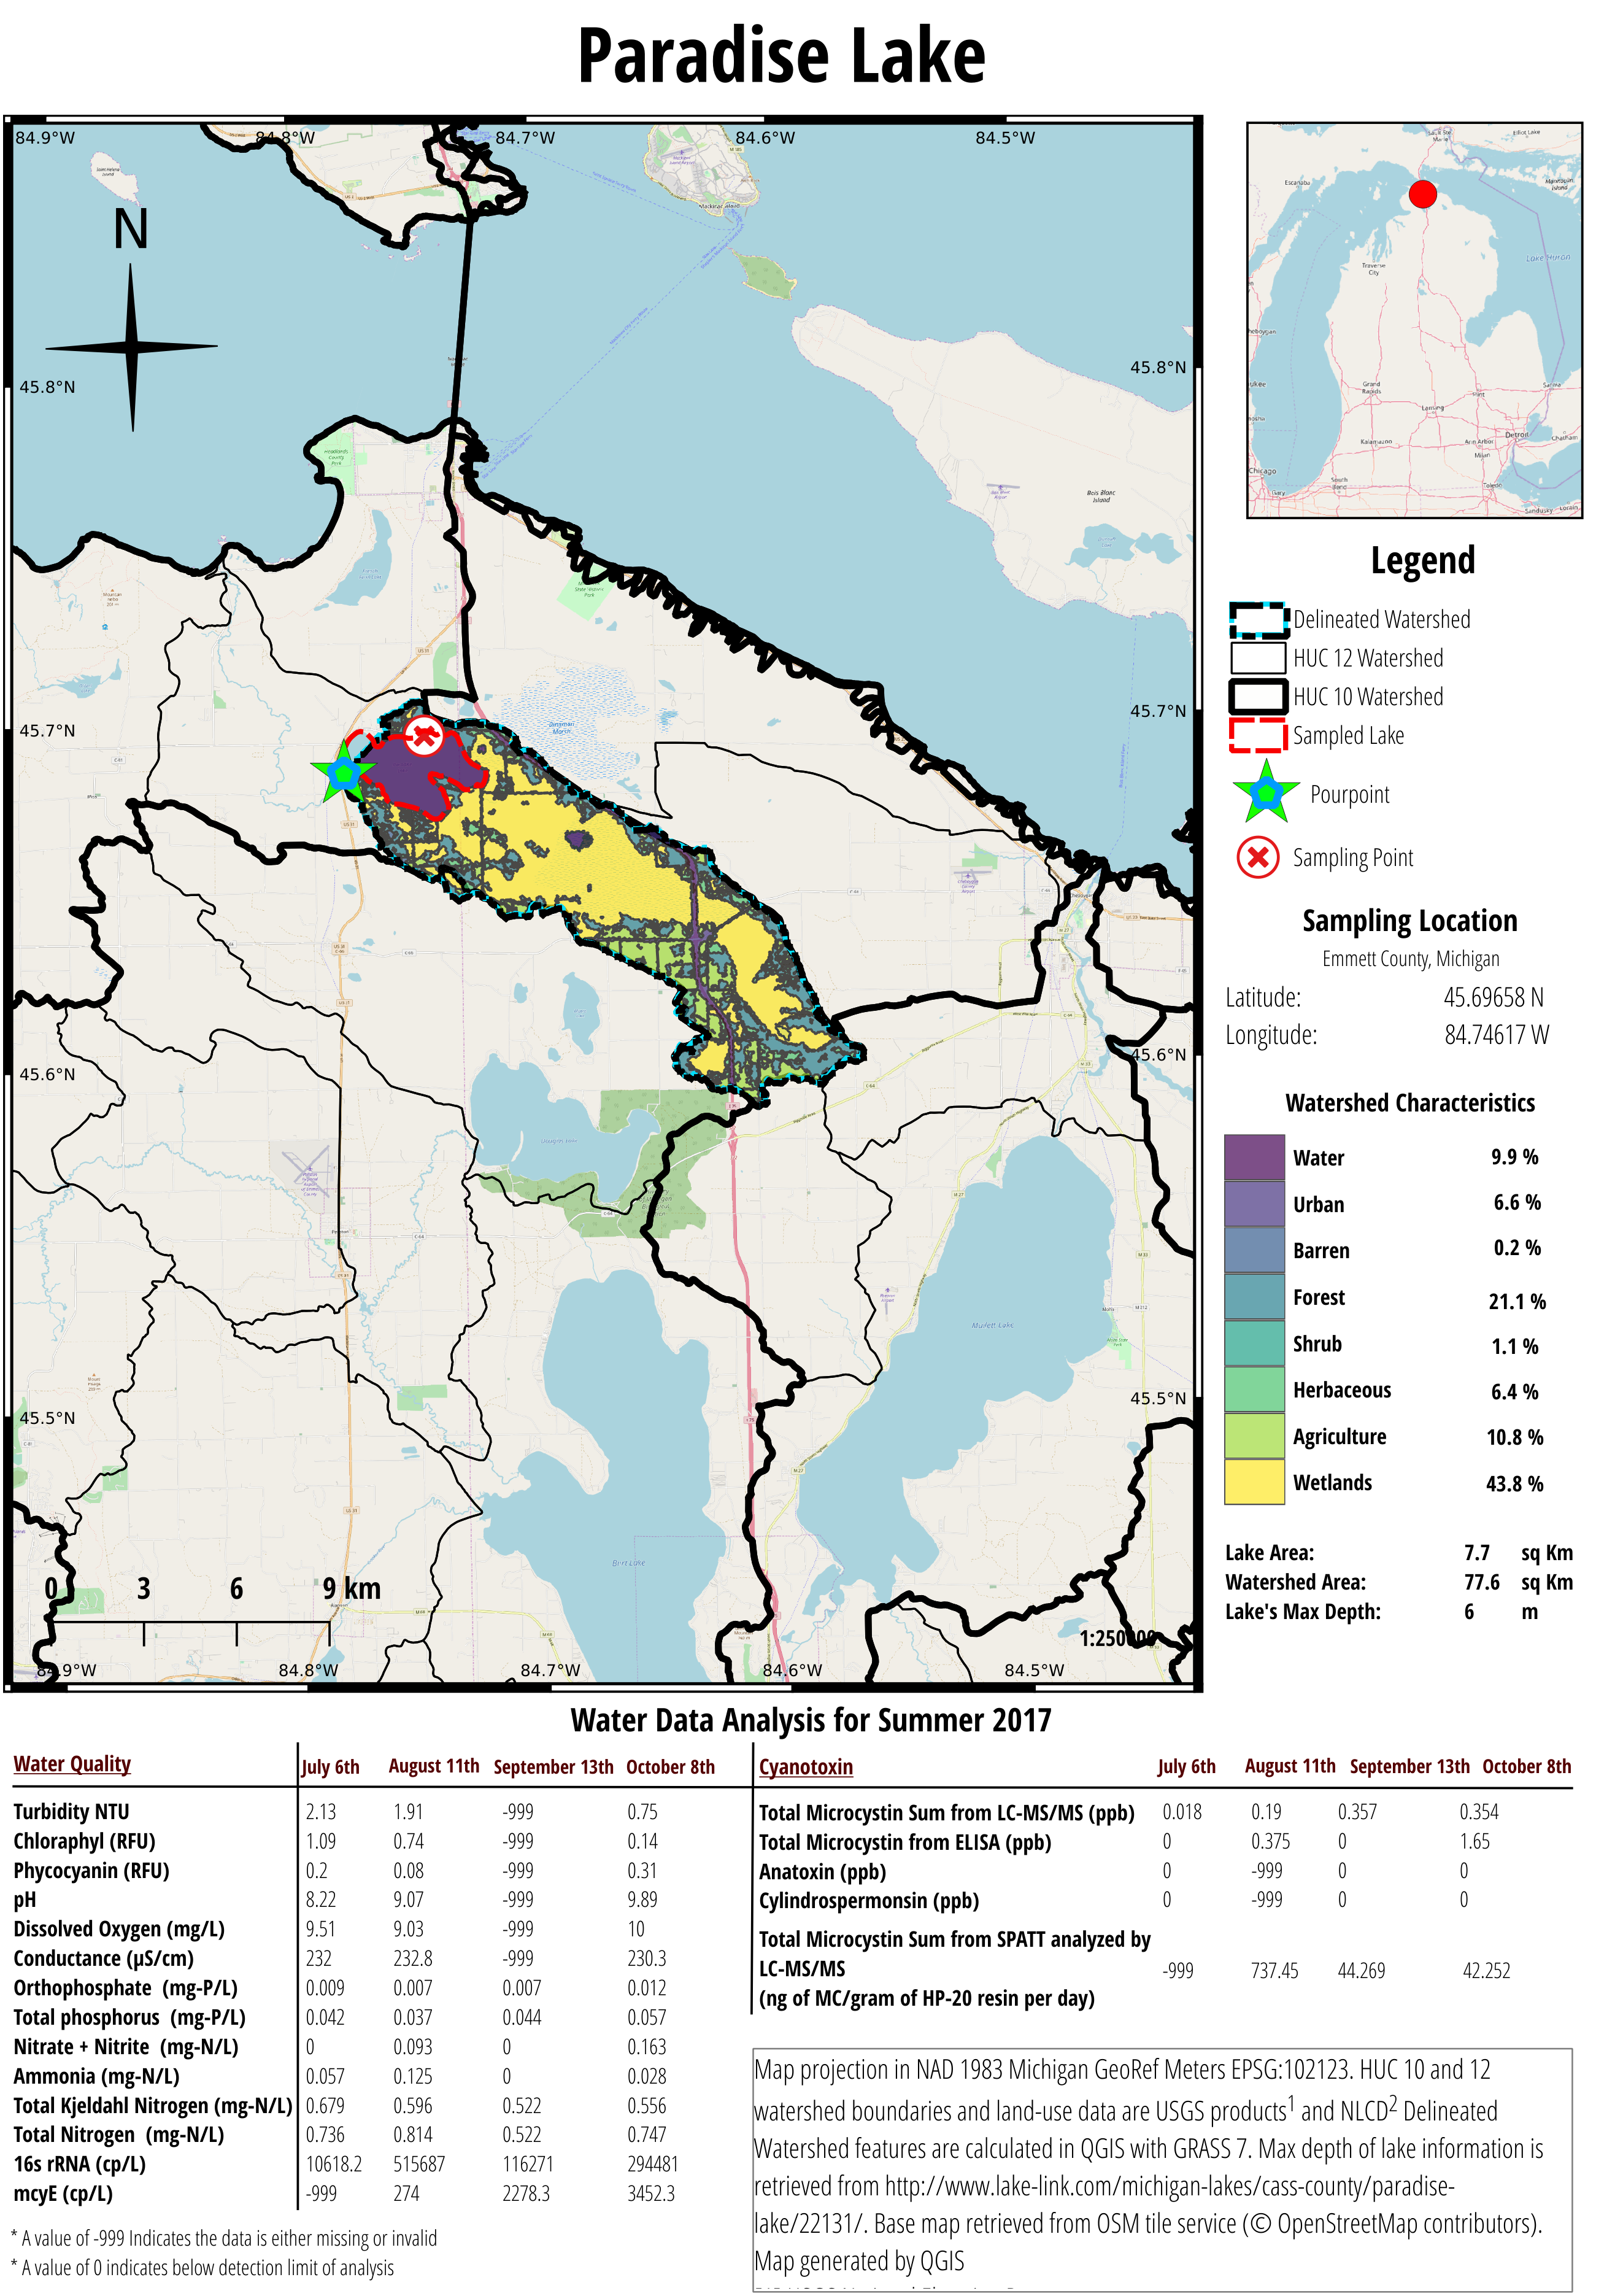
\includegraphics{figures/atlas/output_19}}
  }
\caption{GIS Map of Paradise Lake}
\end{figure}

\begin{figure}[t]
\centerline{%
  \resizebox{\textwidth}{!}{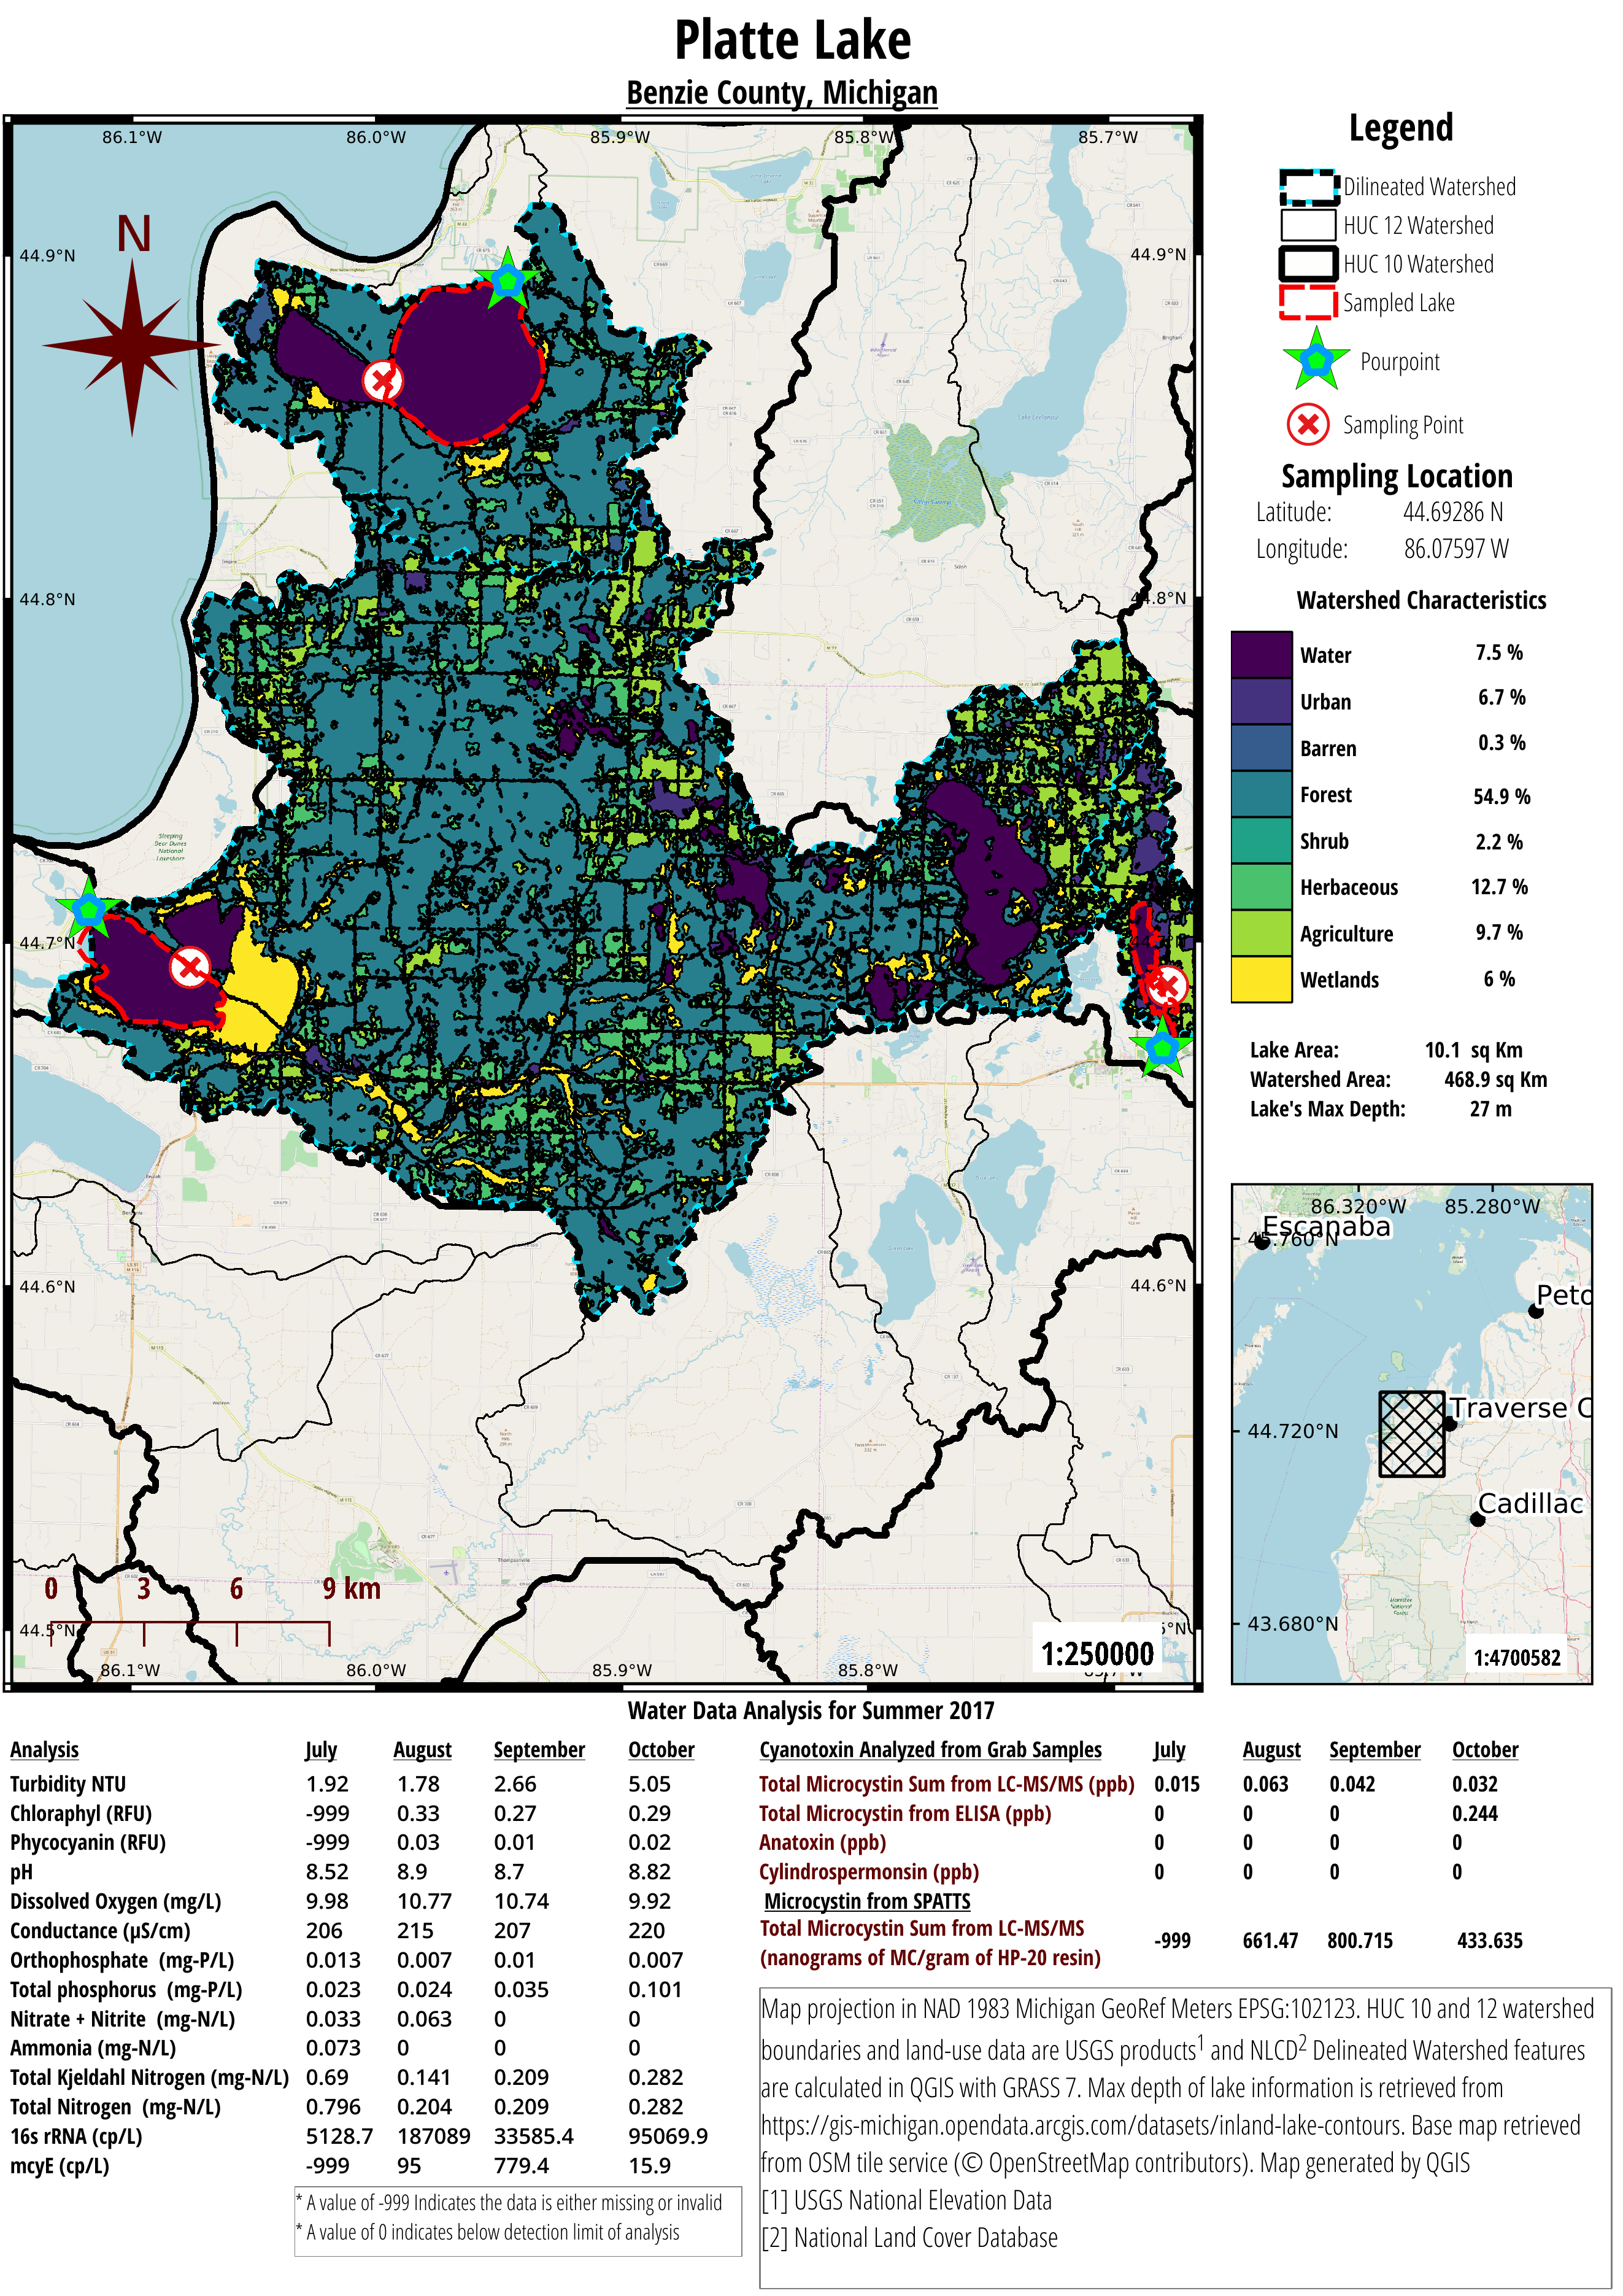
\includegraphics{figures/atlas/output_20}}
  }
\caption{GIS Map of Platte Lake}
\end{figure}

\begin{figure}[t]
\centerline{%
  \resizebox{\textwidth}{!}{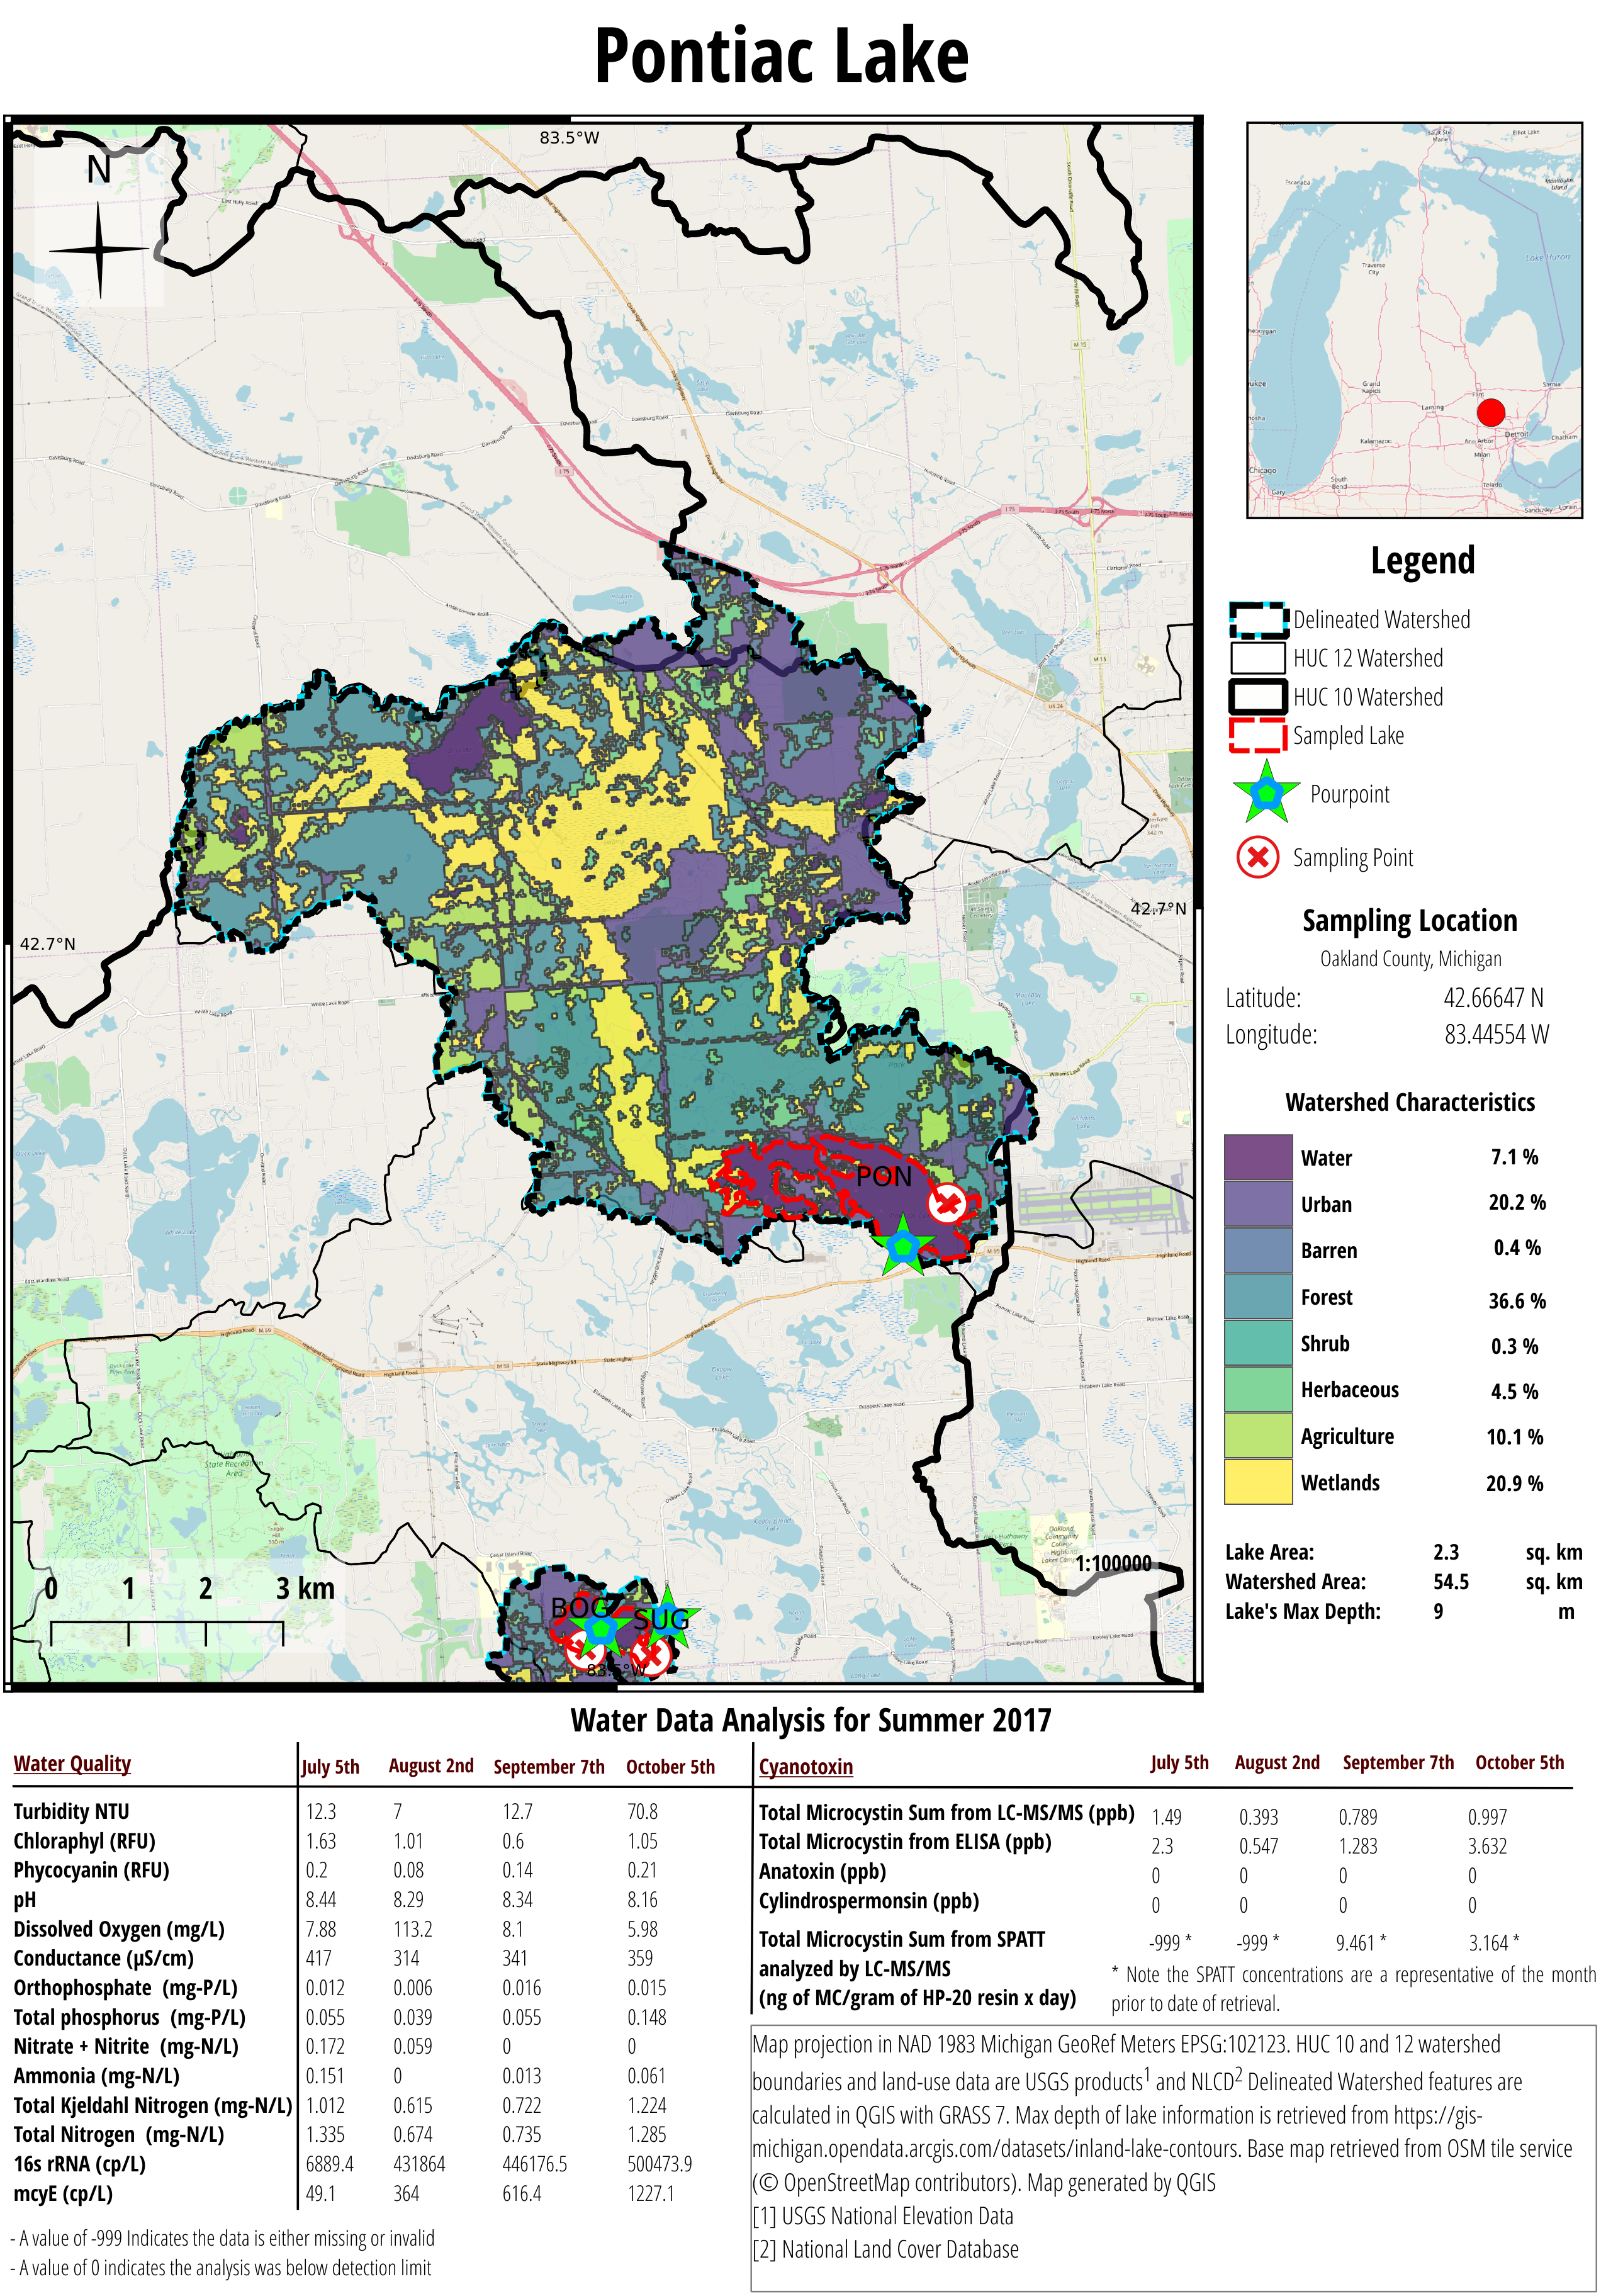
\includegraphics{figures/atlas/output_21}}
  }
\caption{GIS Map of Pontiac Lake}
\end{figure}

\begin{figure}[t]
\centerline{%
  \resizebox{\textwidth}{!}{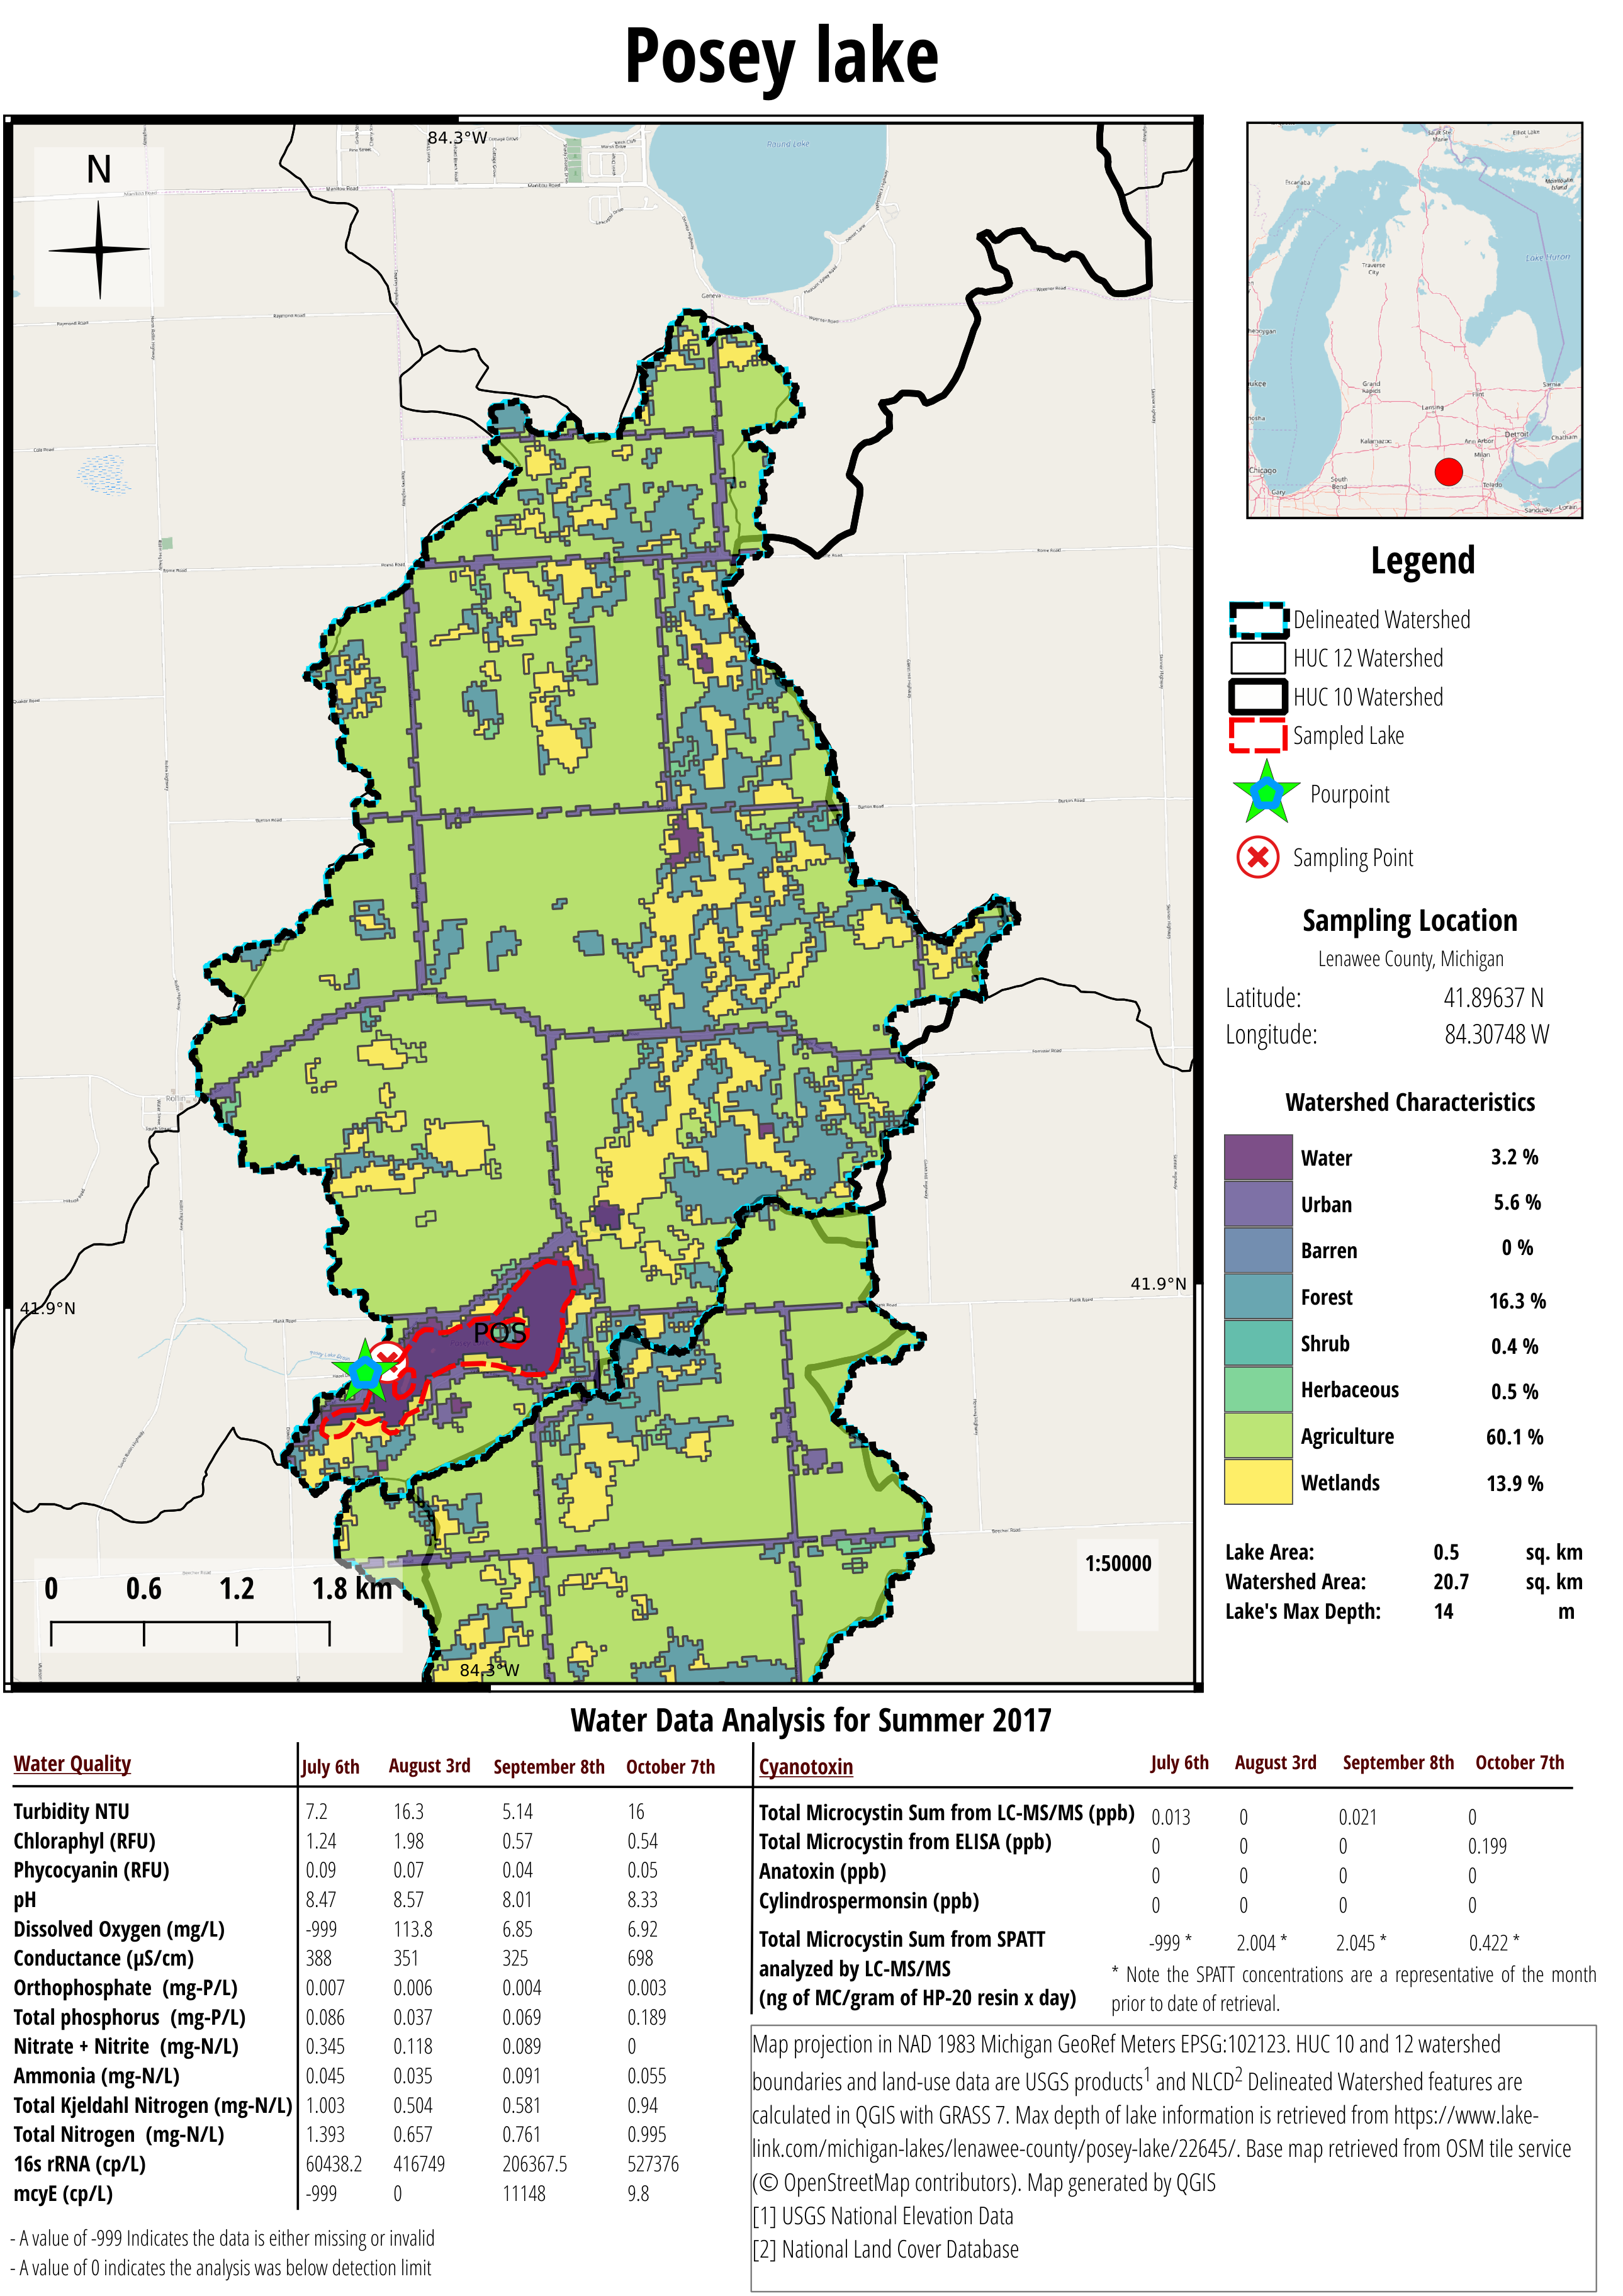
\includegraphics{figures/atlas/output_22}}
  }
\caption{GIS Map of Posey Lake}
\end{figure}

\begin{figure}[t]
\centerline{%
  \resizebox{\textwidth}{!}{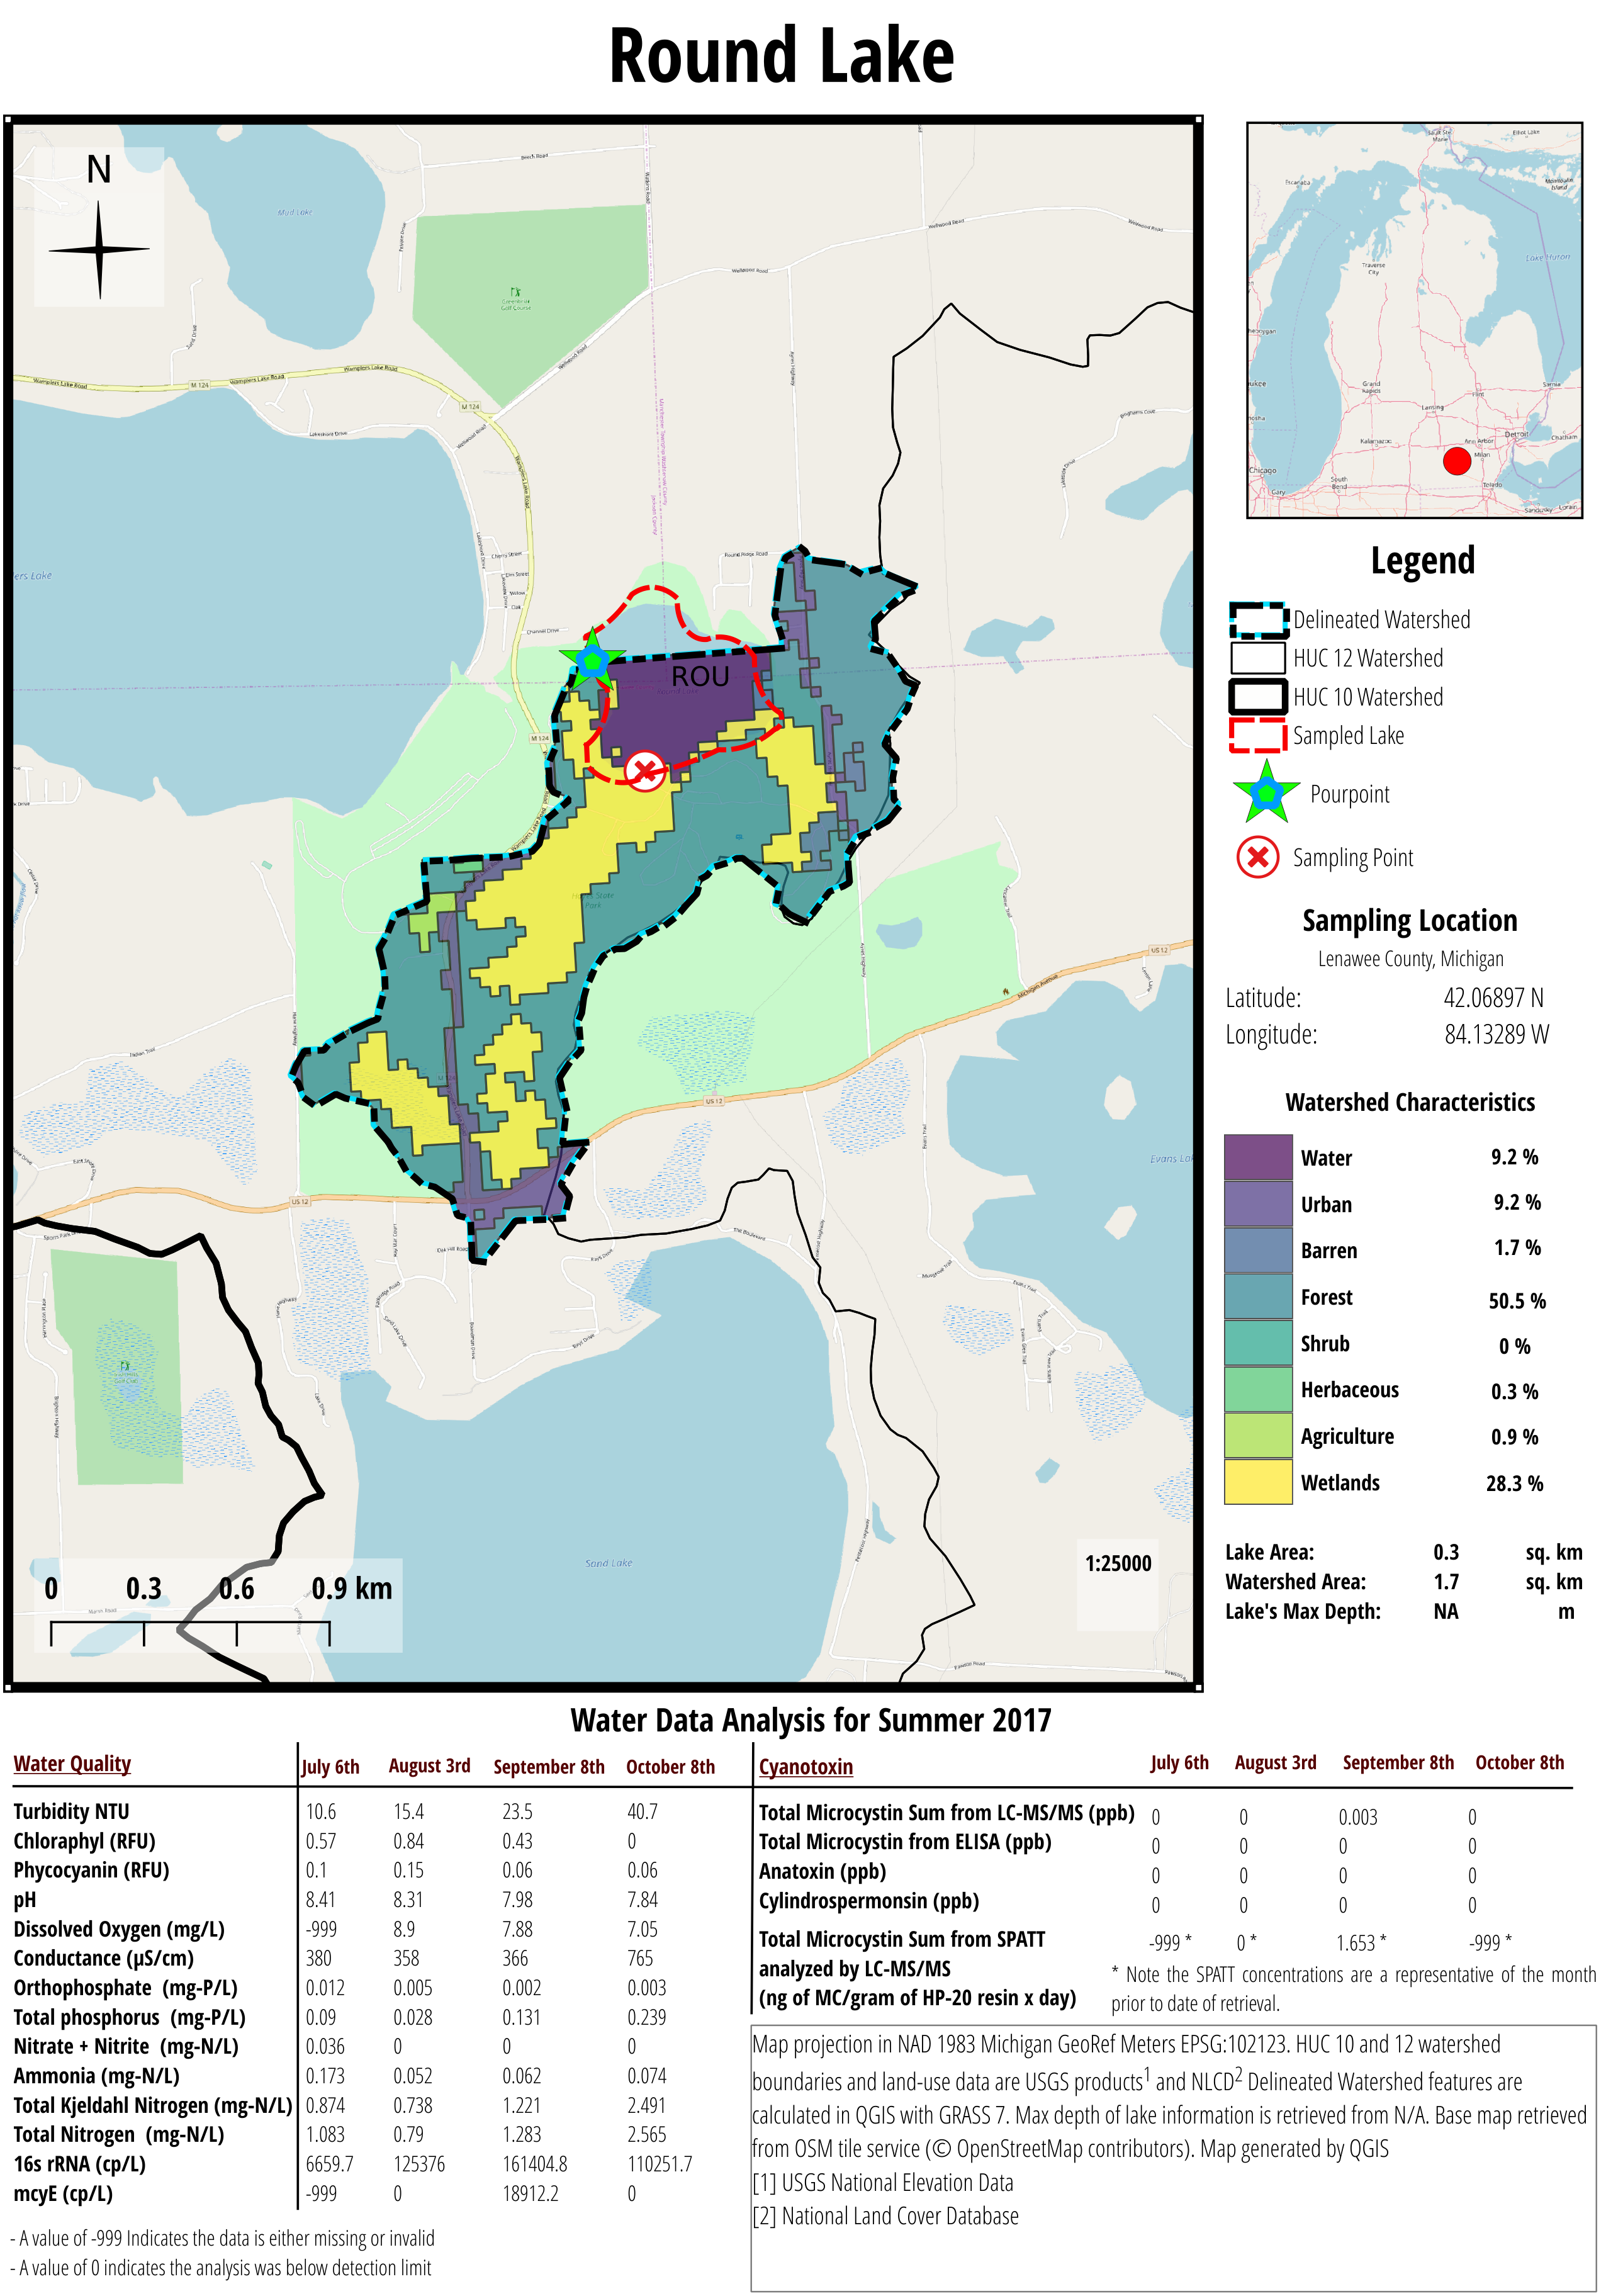
\includegraphics{figures/atlas/output_23}}
  }
\caption{GIS Map of Round Lake}
\end{figure}

\begin{figure}[t]
\centerline{%
  \resizebox{\textwidth}{!}{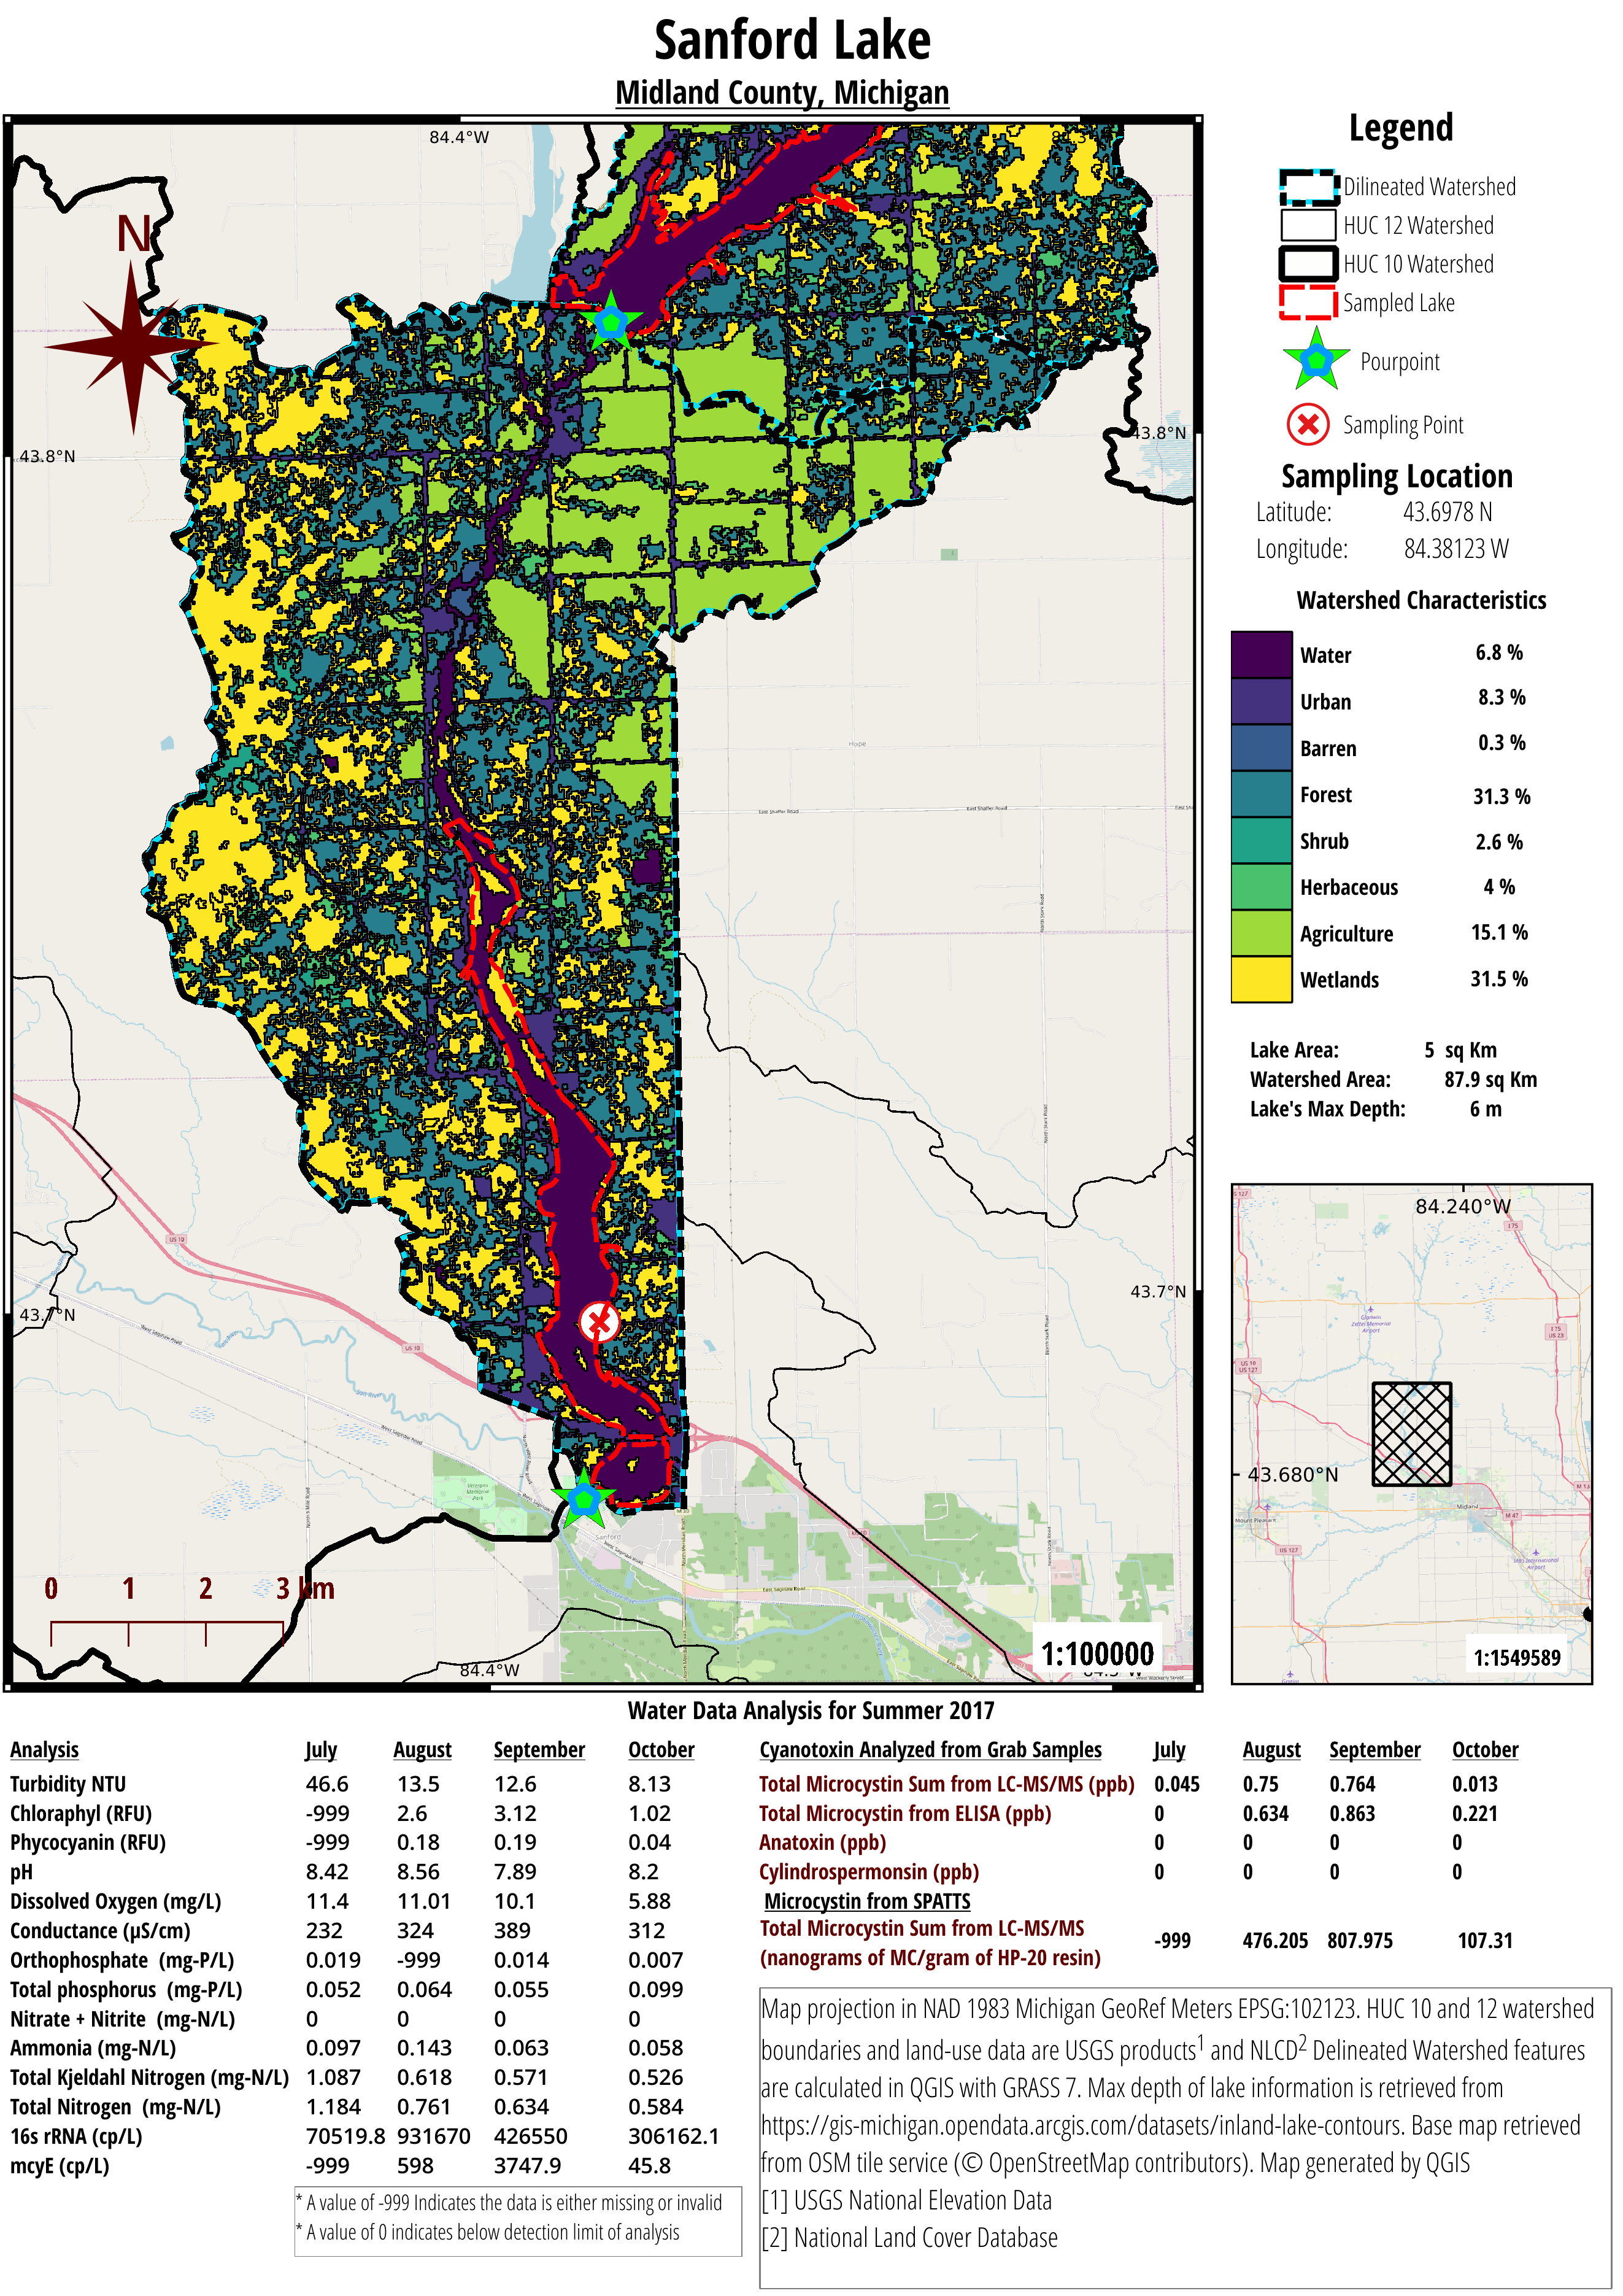
\includegraphics{figures/atlas/output_24}}
  }
\caption{GIS Map of Sanford Lake}
\end{figure}

\begin{figure}[t]
\centerline{%
  \resizebox{\textwidth}{!}{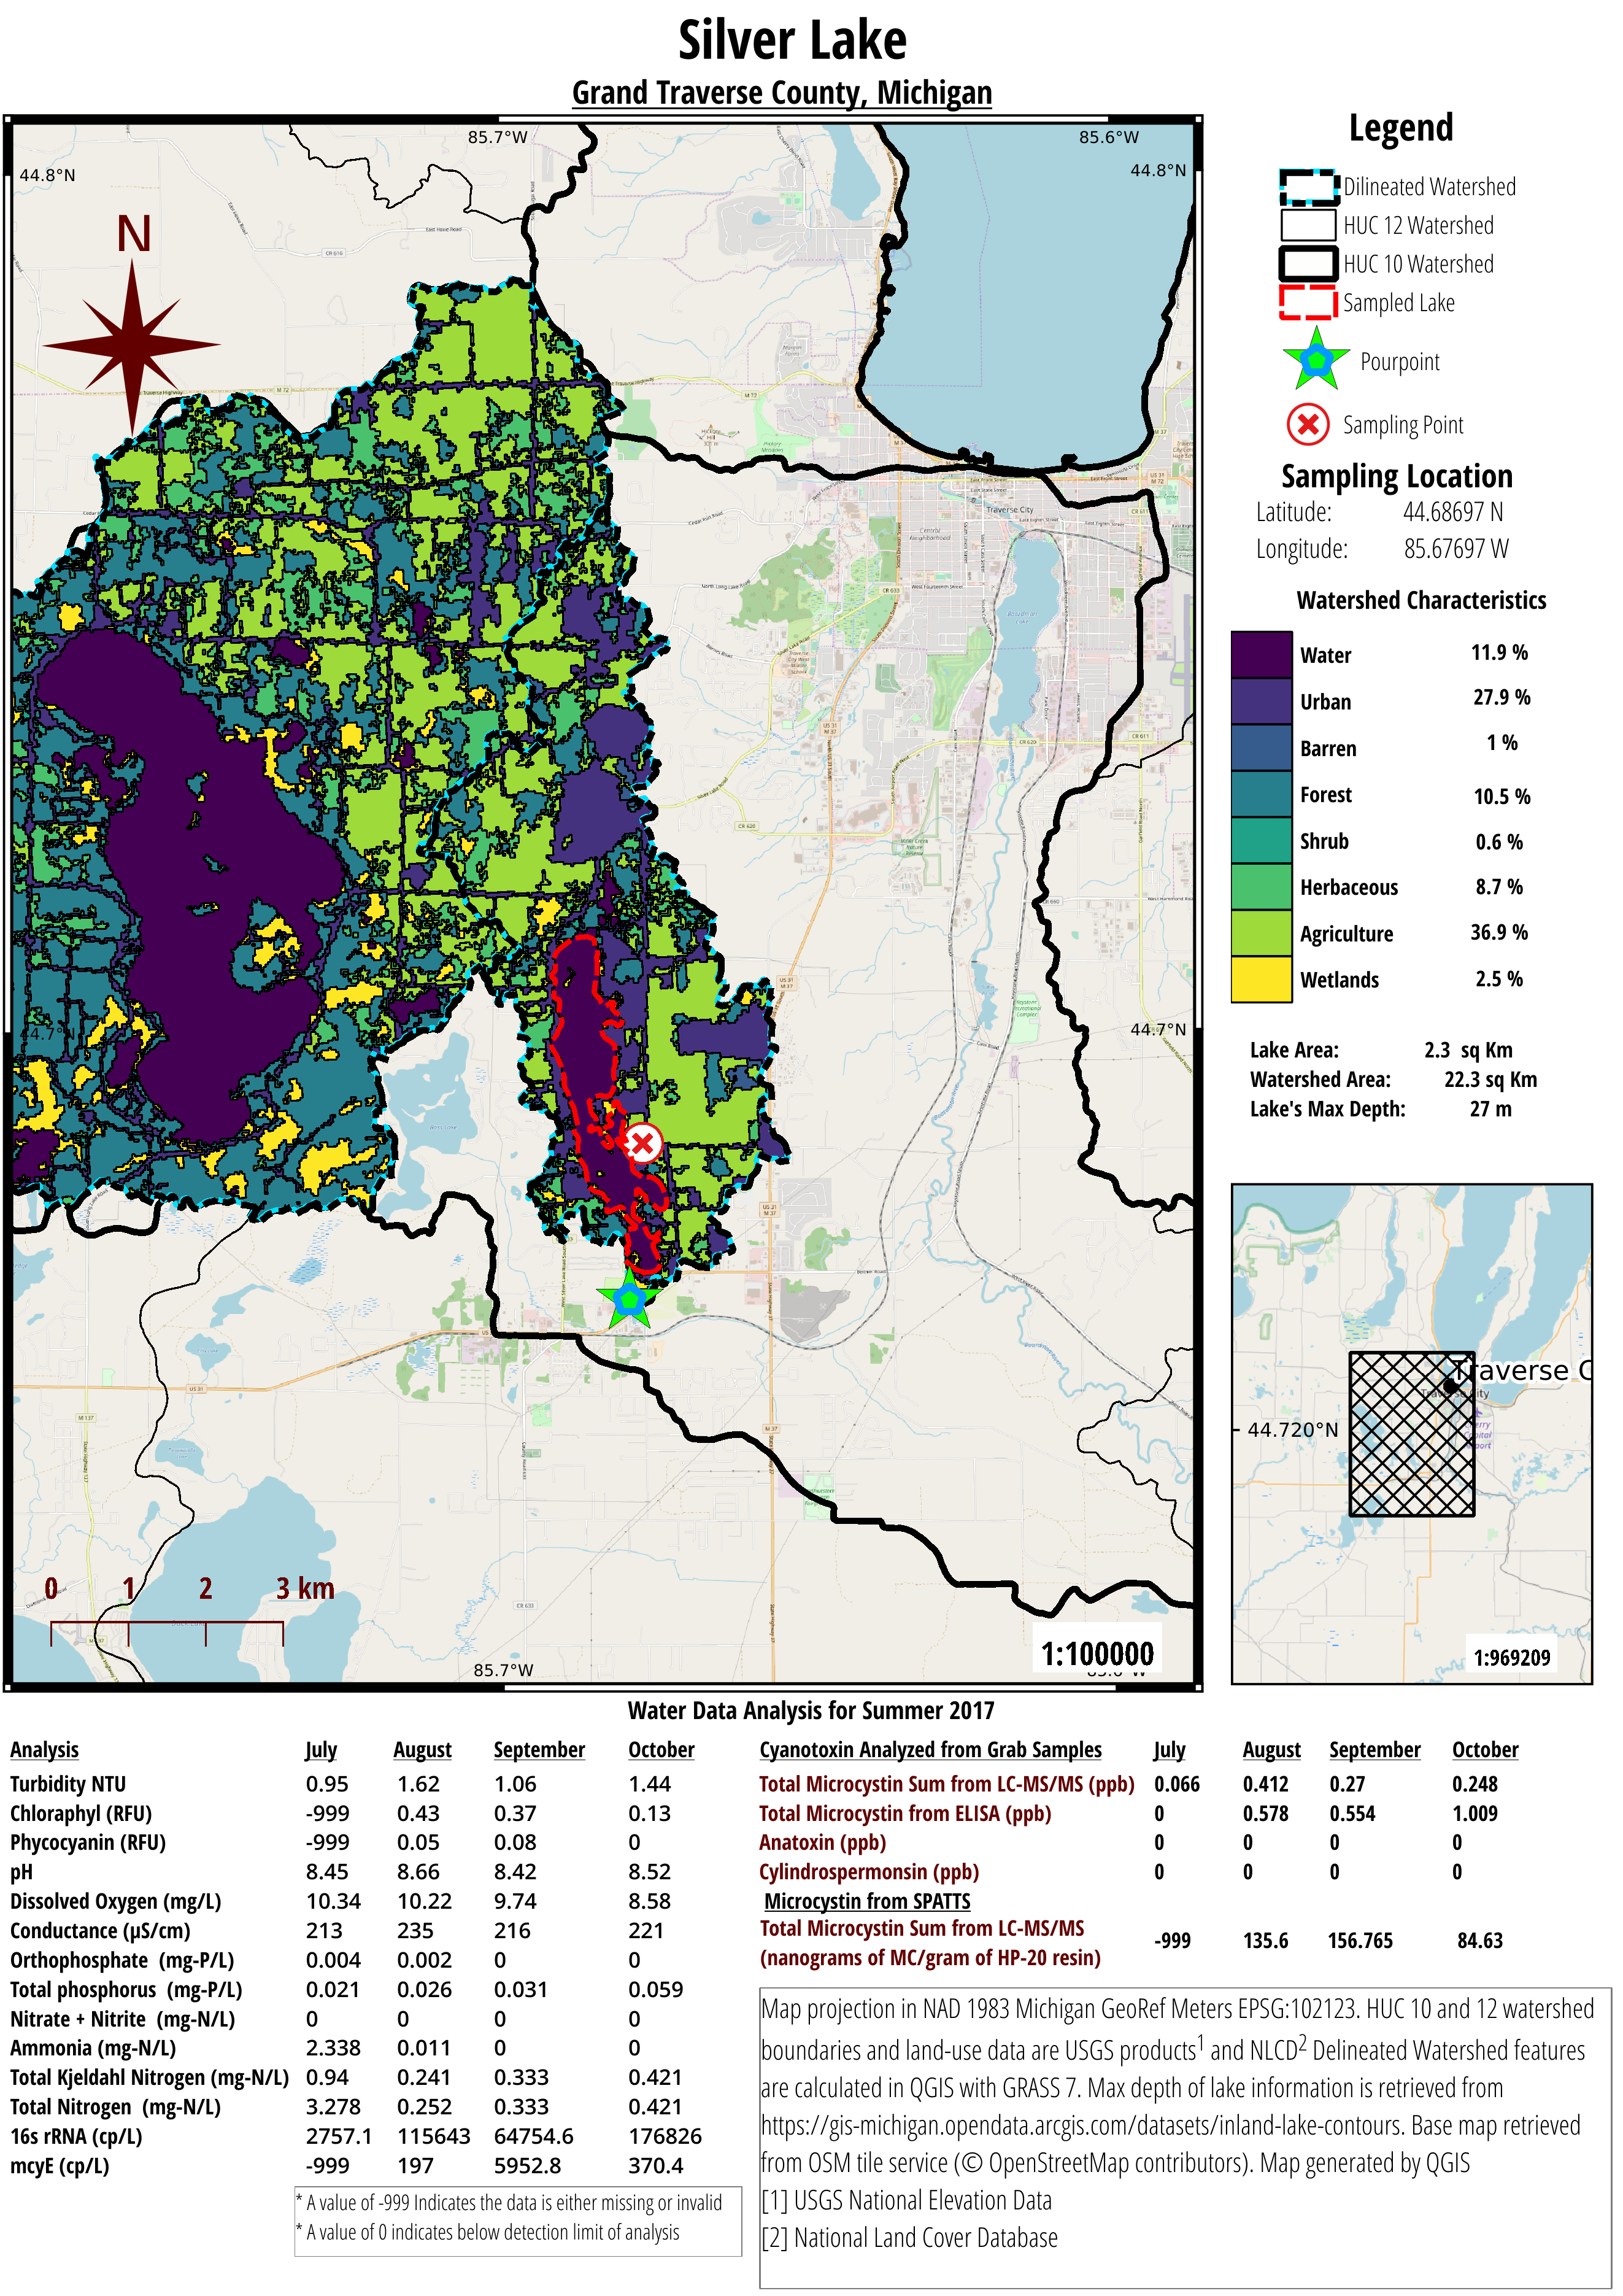
\includegraphics{figures/atlas/output_25}}
  }
\caption{GIS Map of Silver Lake}
\end{figure}

\begin{figure}[t]
\centerline{%
  \resizebox{\textwidth}{!}{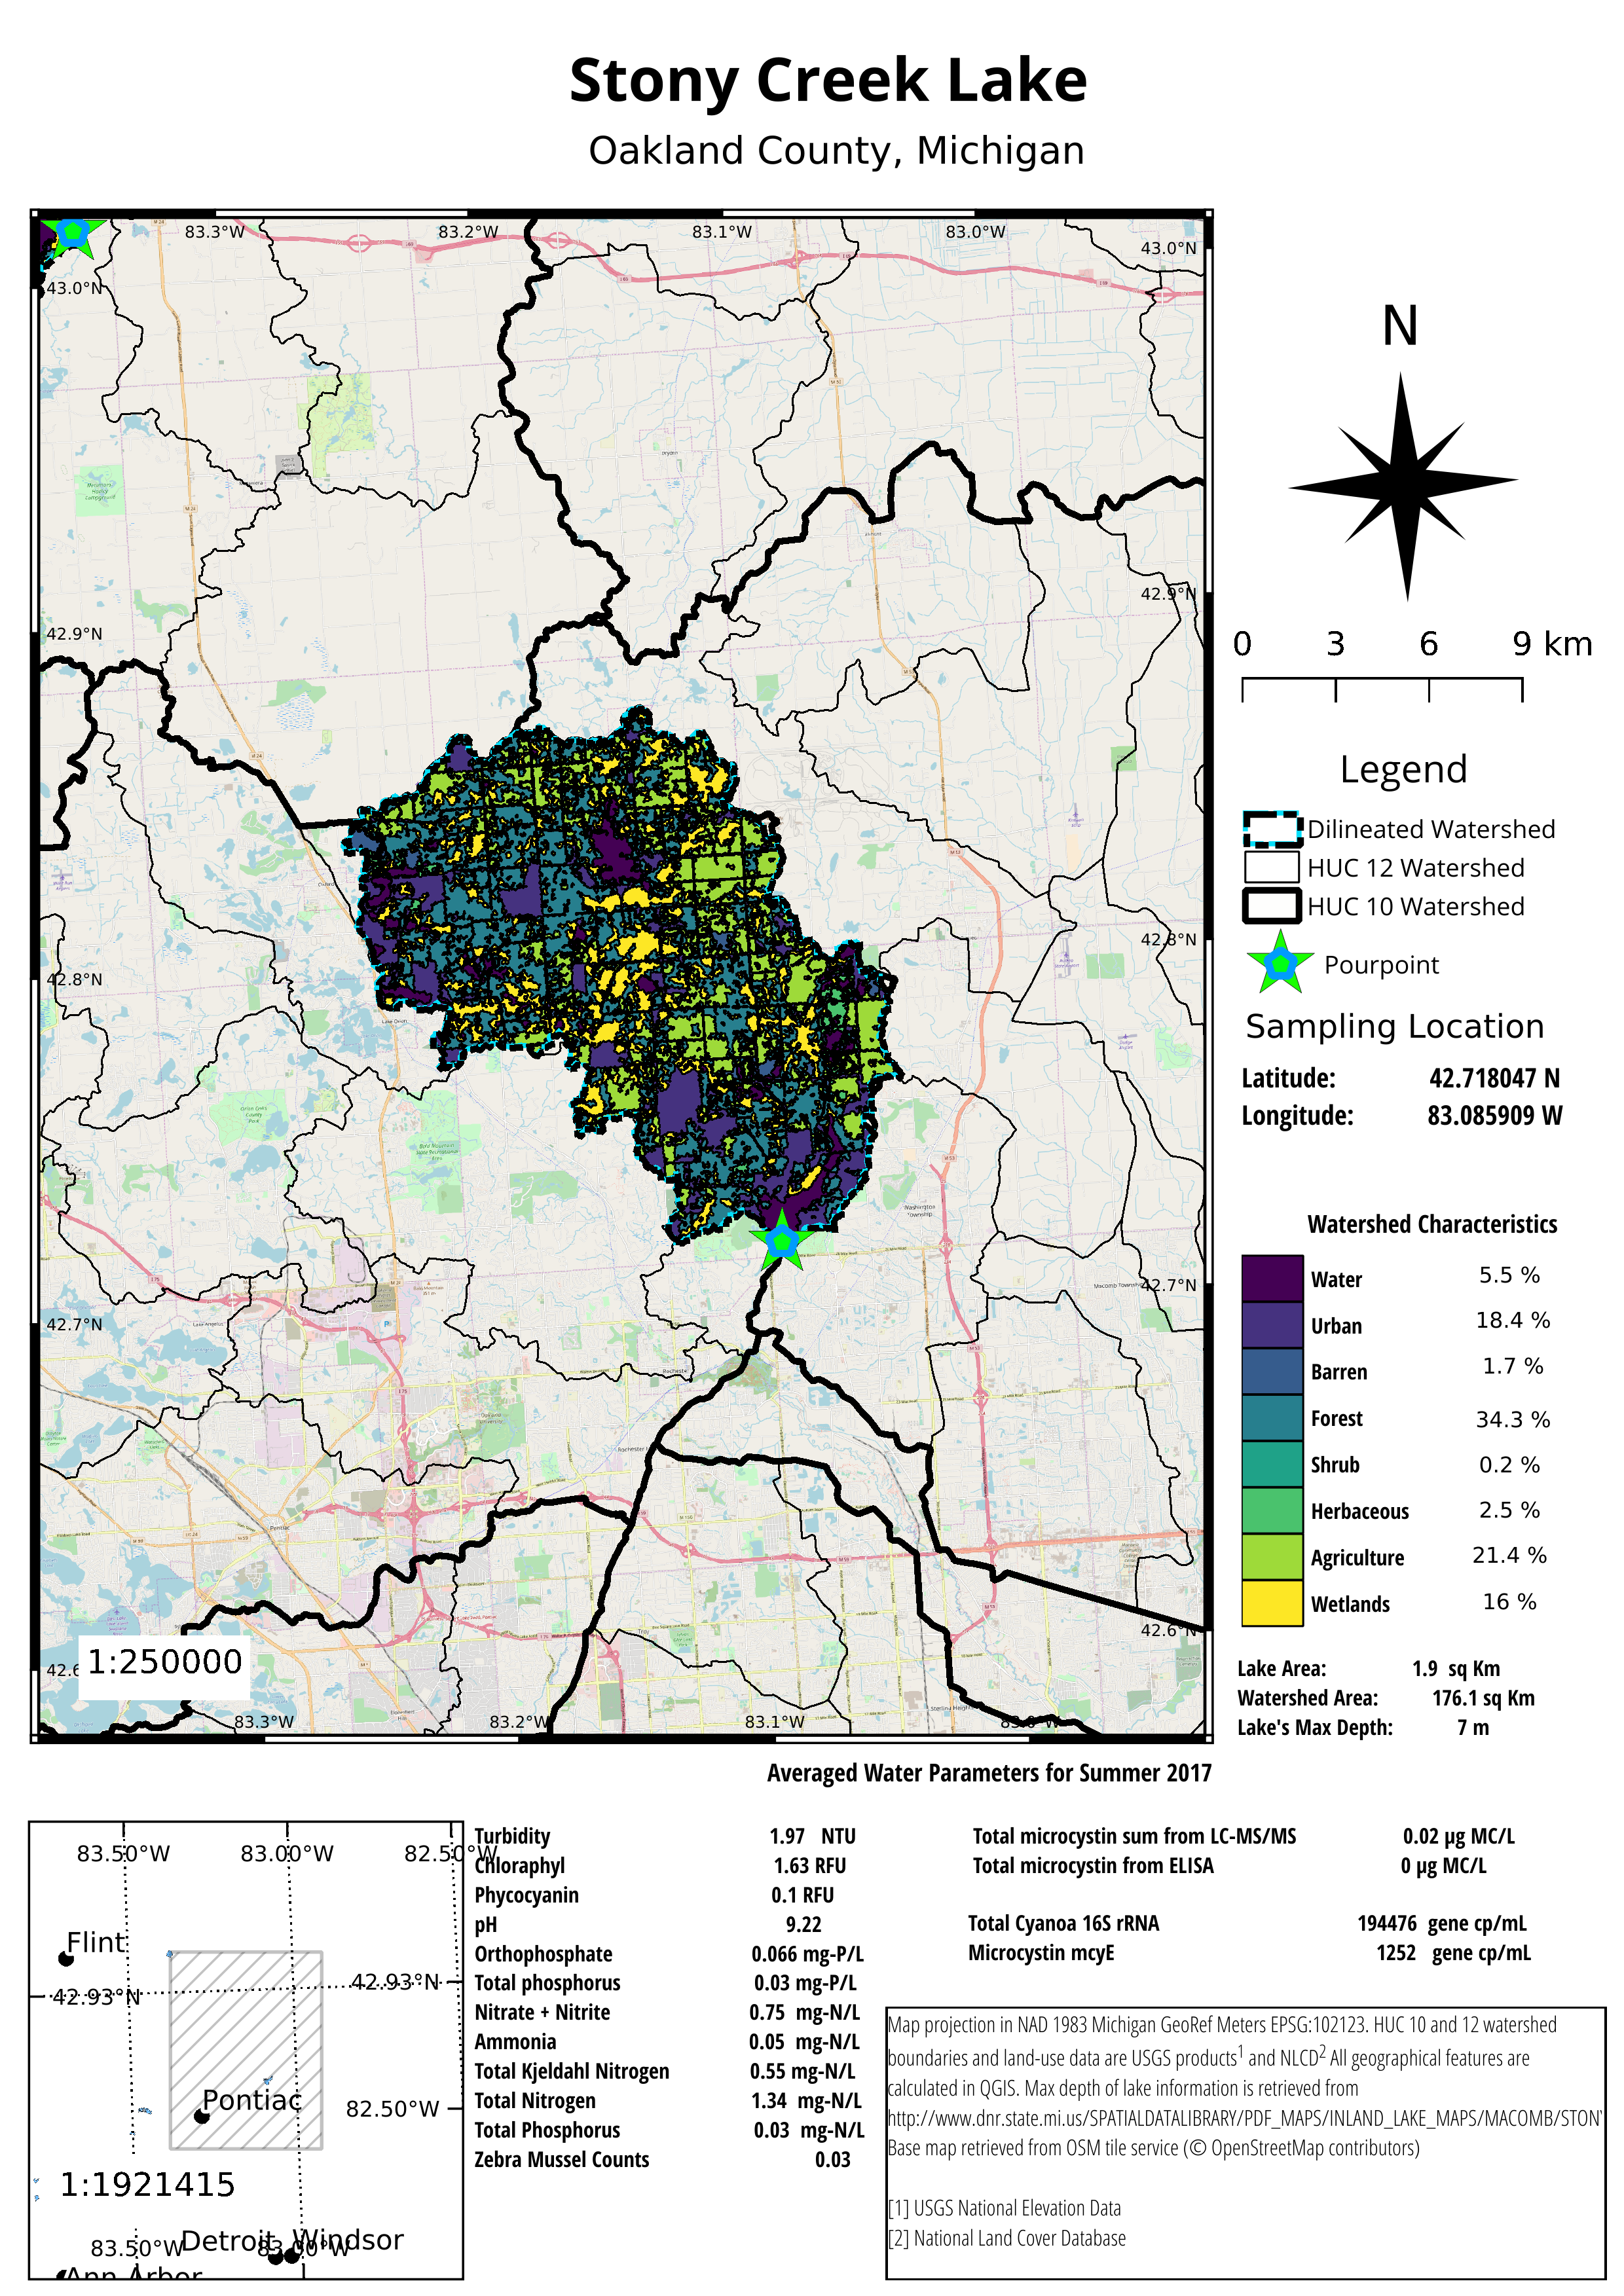
\includegraphics{figures/atlas/output_26}}
  }
\caption{GIS Map of Stoney Lake}
\end{figure}

\begin{figure}[t]
\centerline{%
  \resizebox{\textwidth}{!}{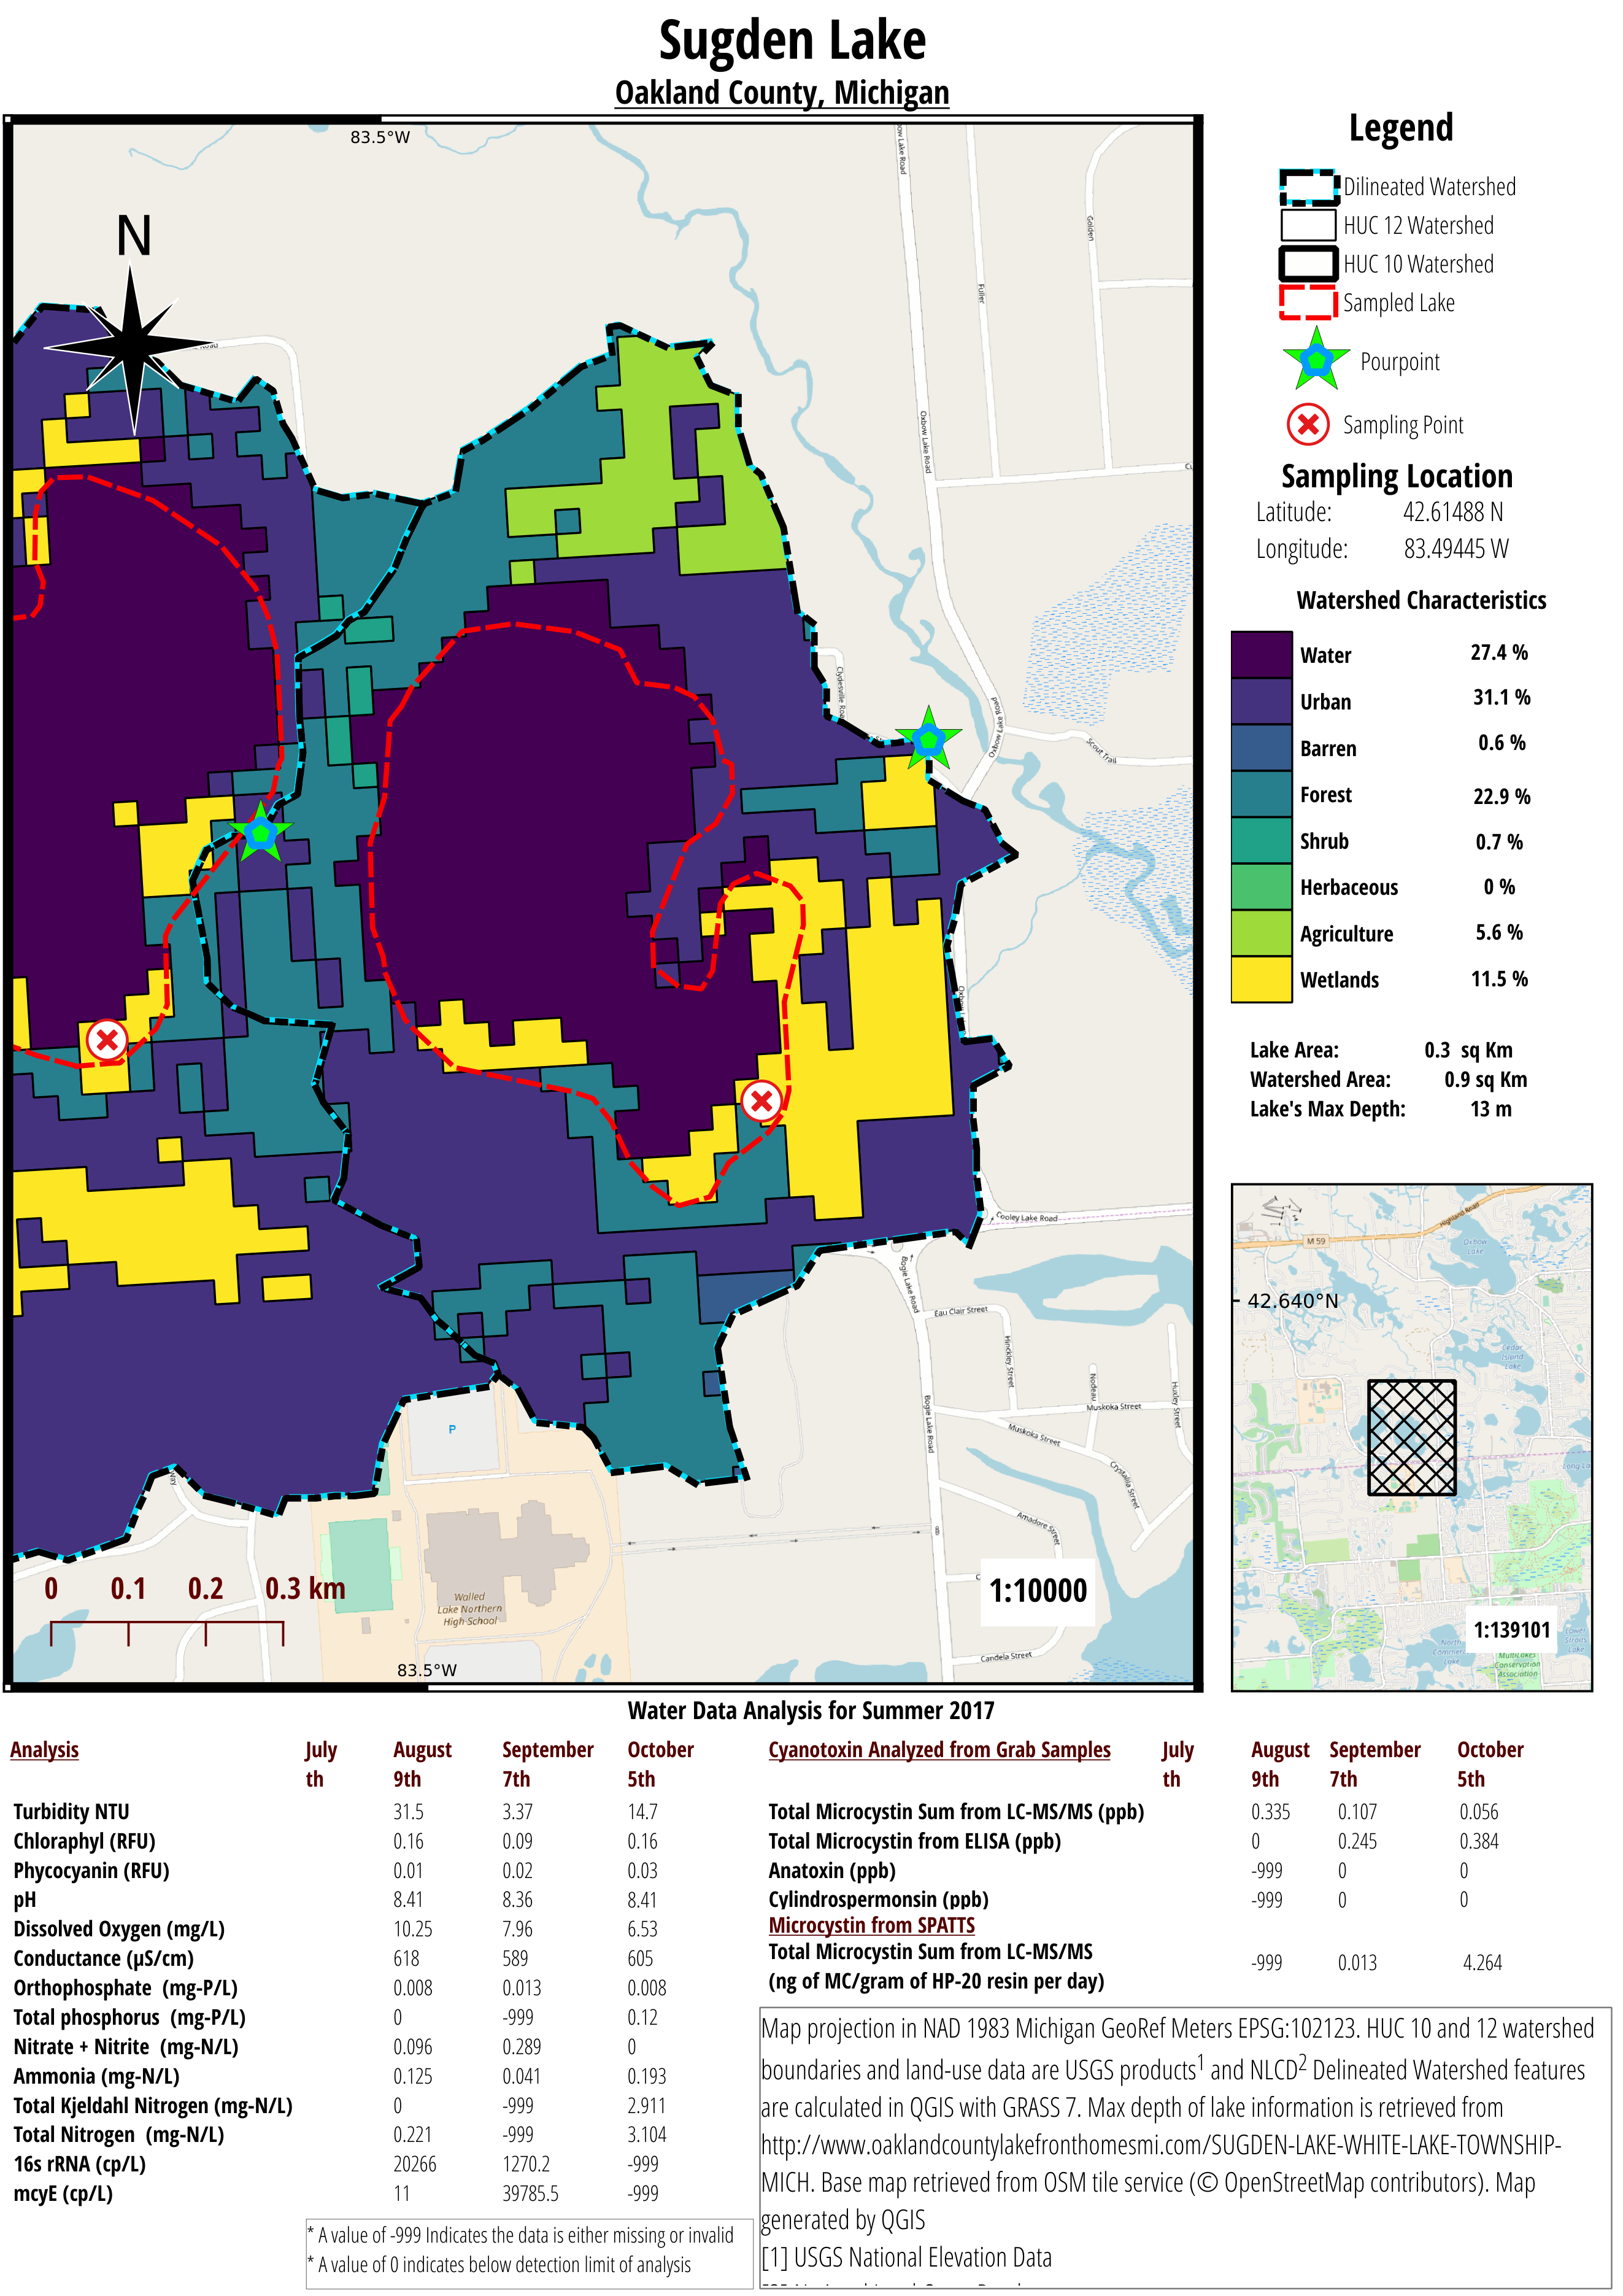
\includegraphics{figures/atlas/output_27}}
  }
\caption{GIS Map of Sugden Lake}
\end{figure}

\begin{figure}[t]
\centerline{%
  \resizebox{\textwidth}{!}{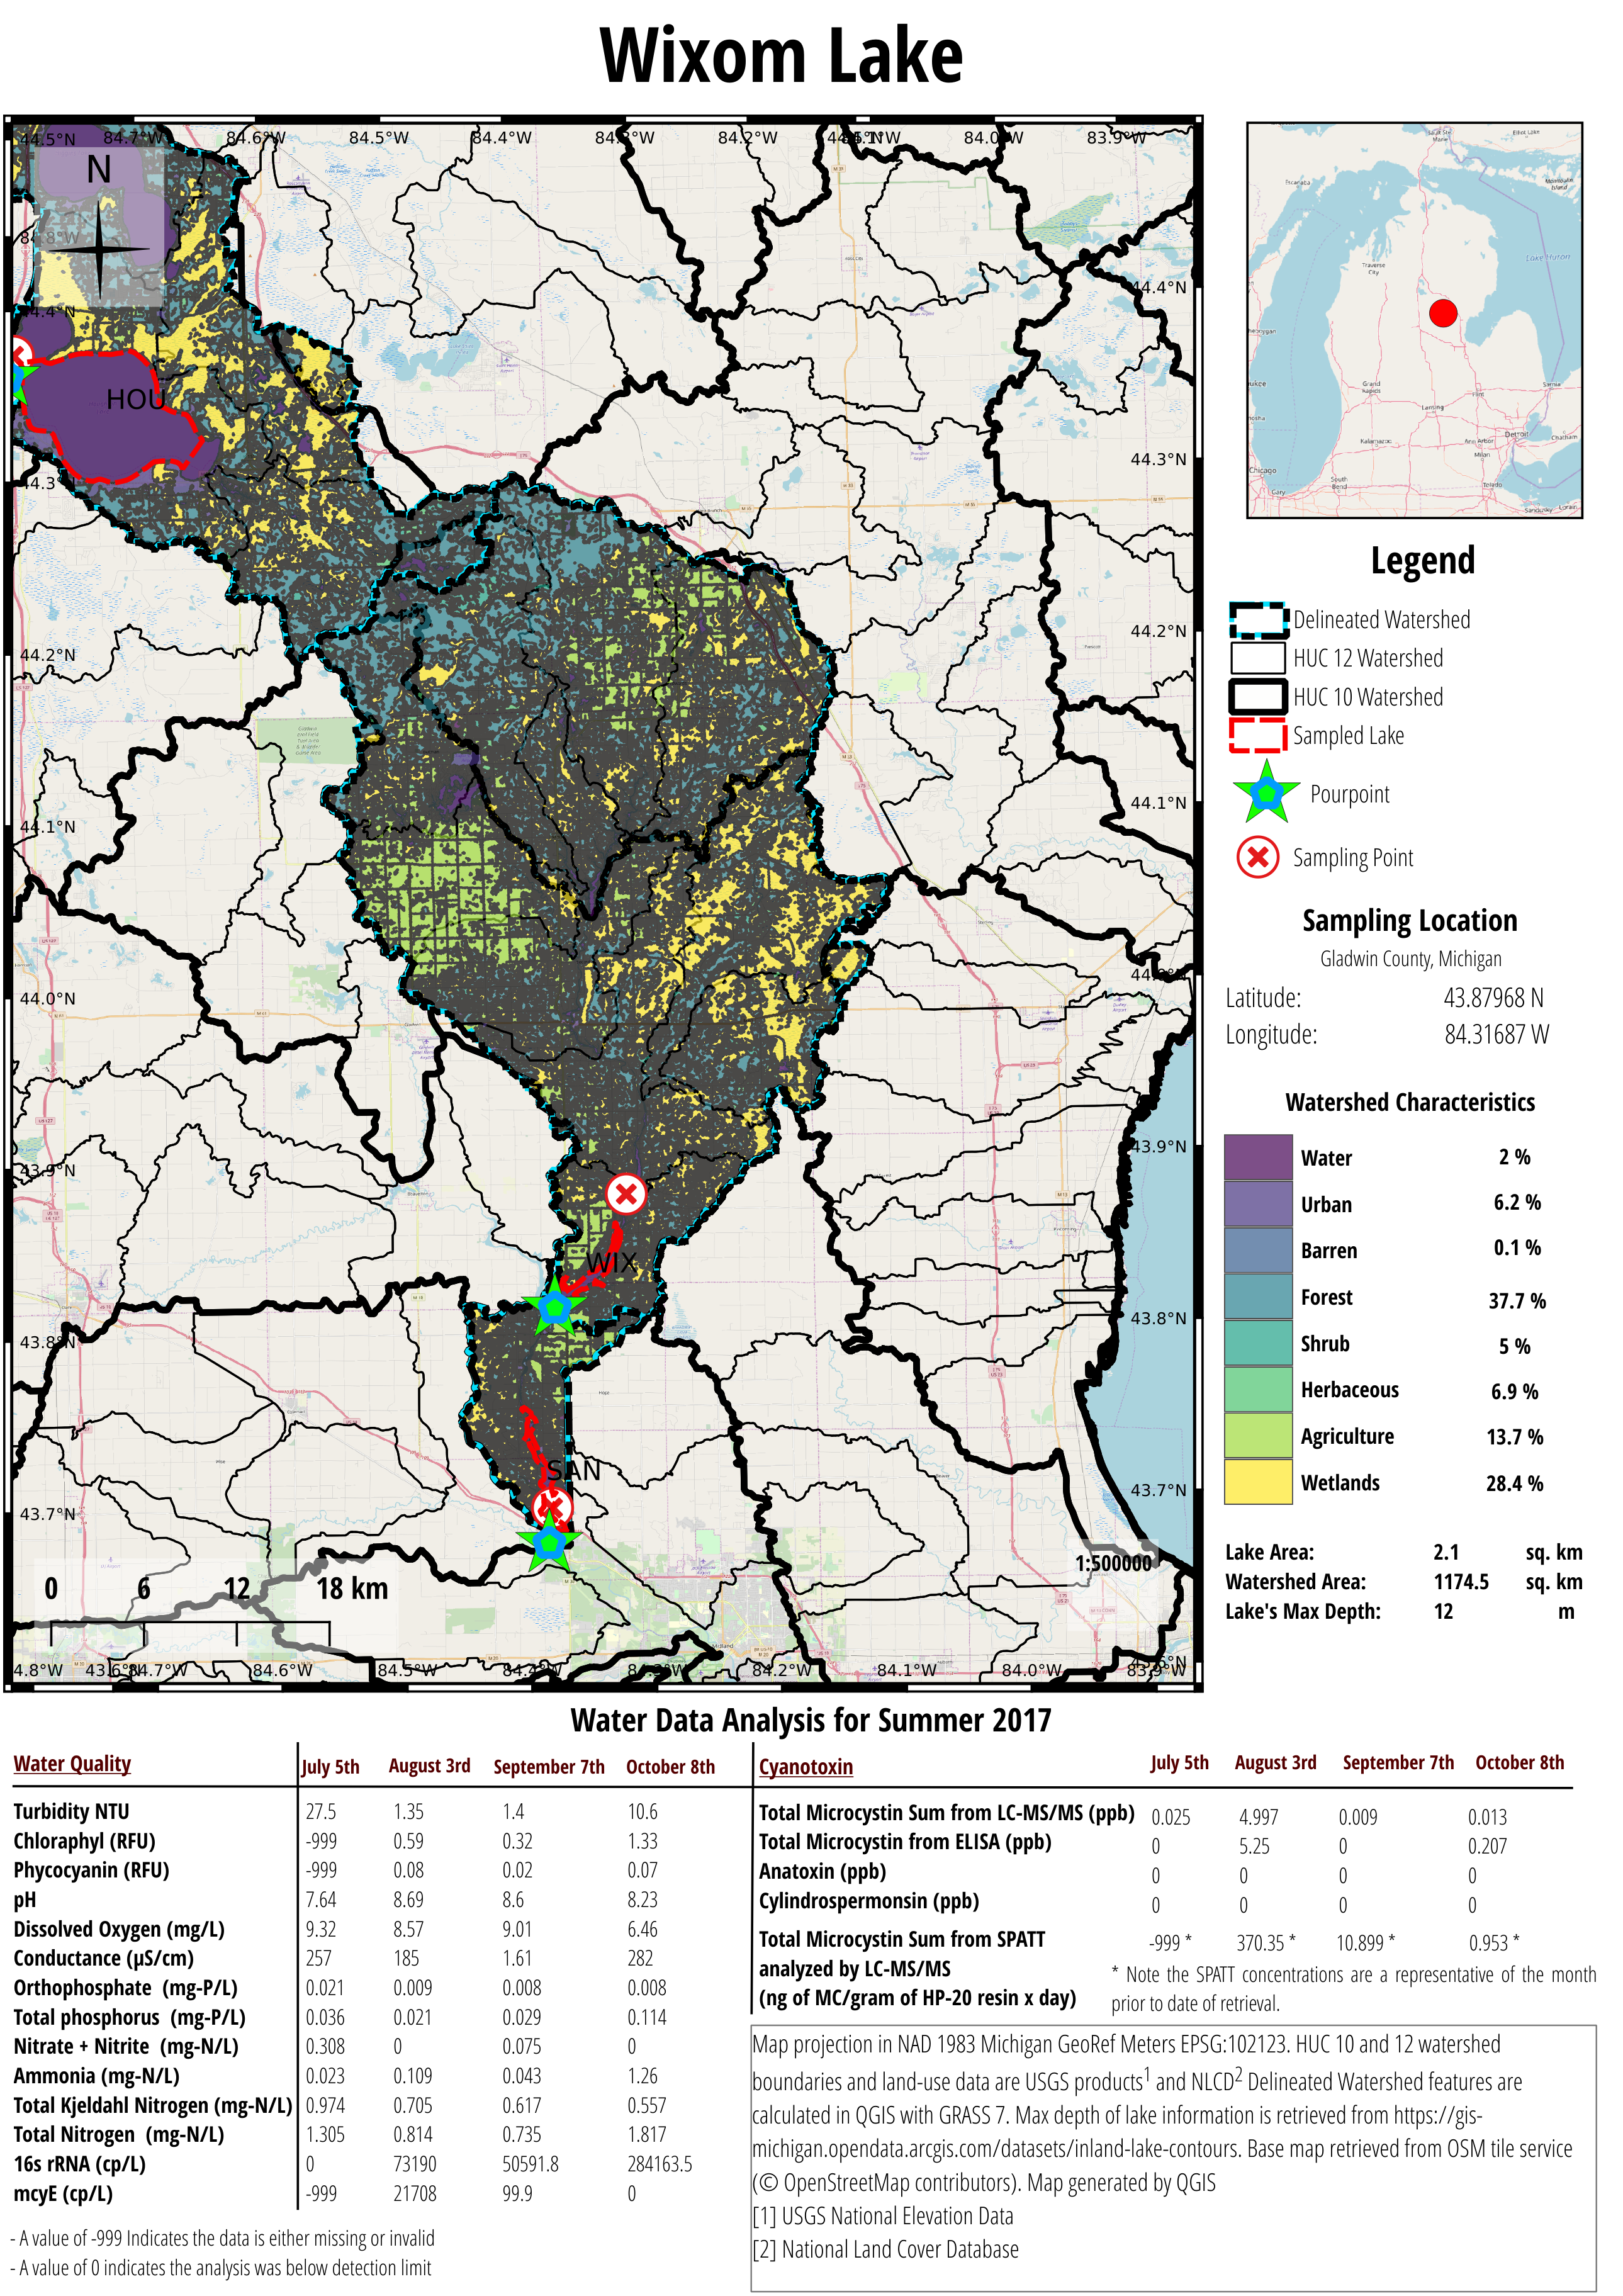
\includegraphics{figures/atlas/output_28}}
  }
\caption{GIS Map of Wixom Lake}
\end{figure}

\begin{figure}[t]
\centerline{%
  \resizebox{\textwidth}{!}{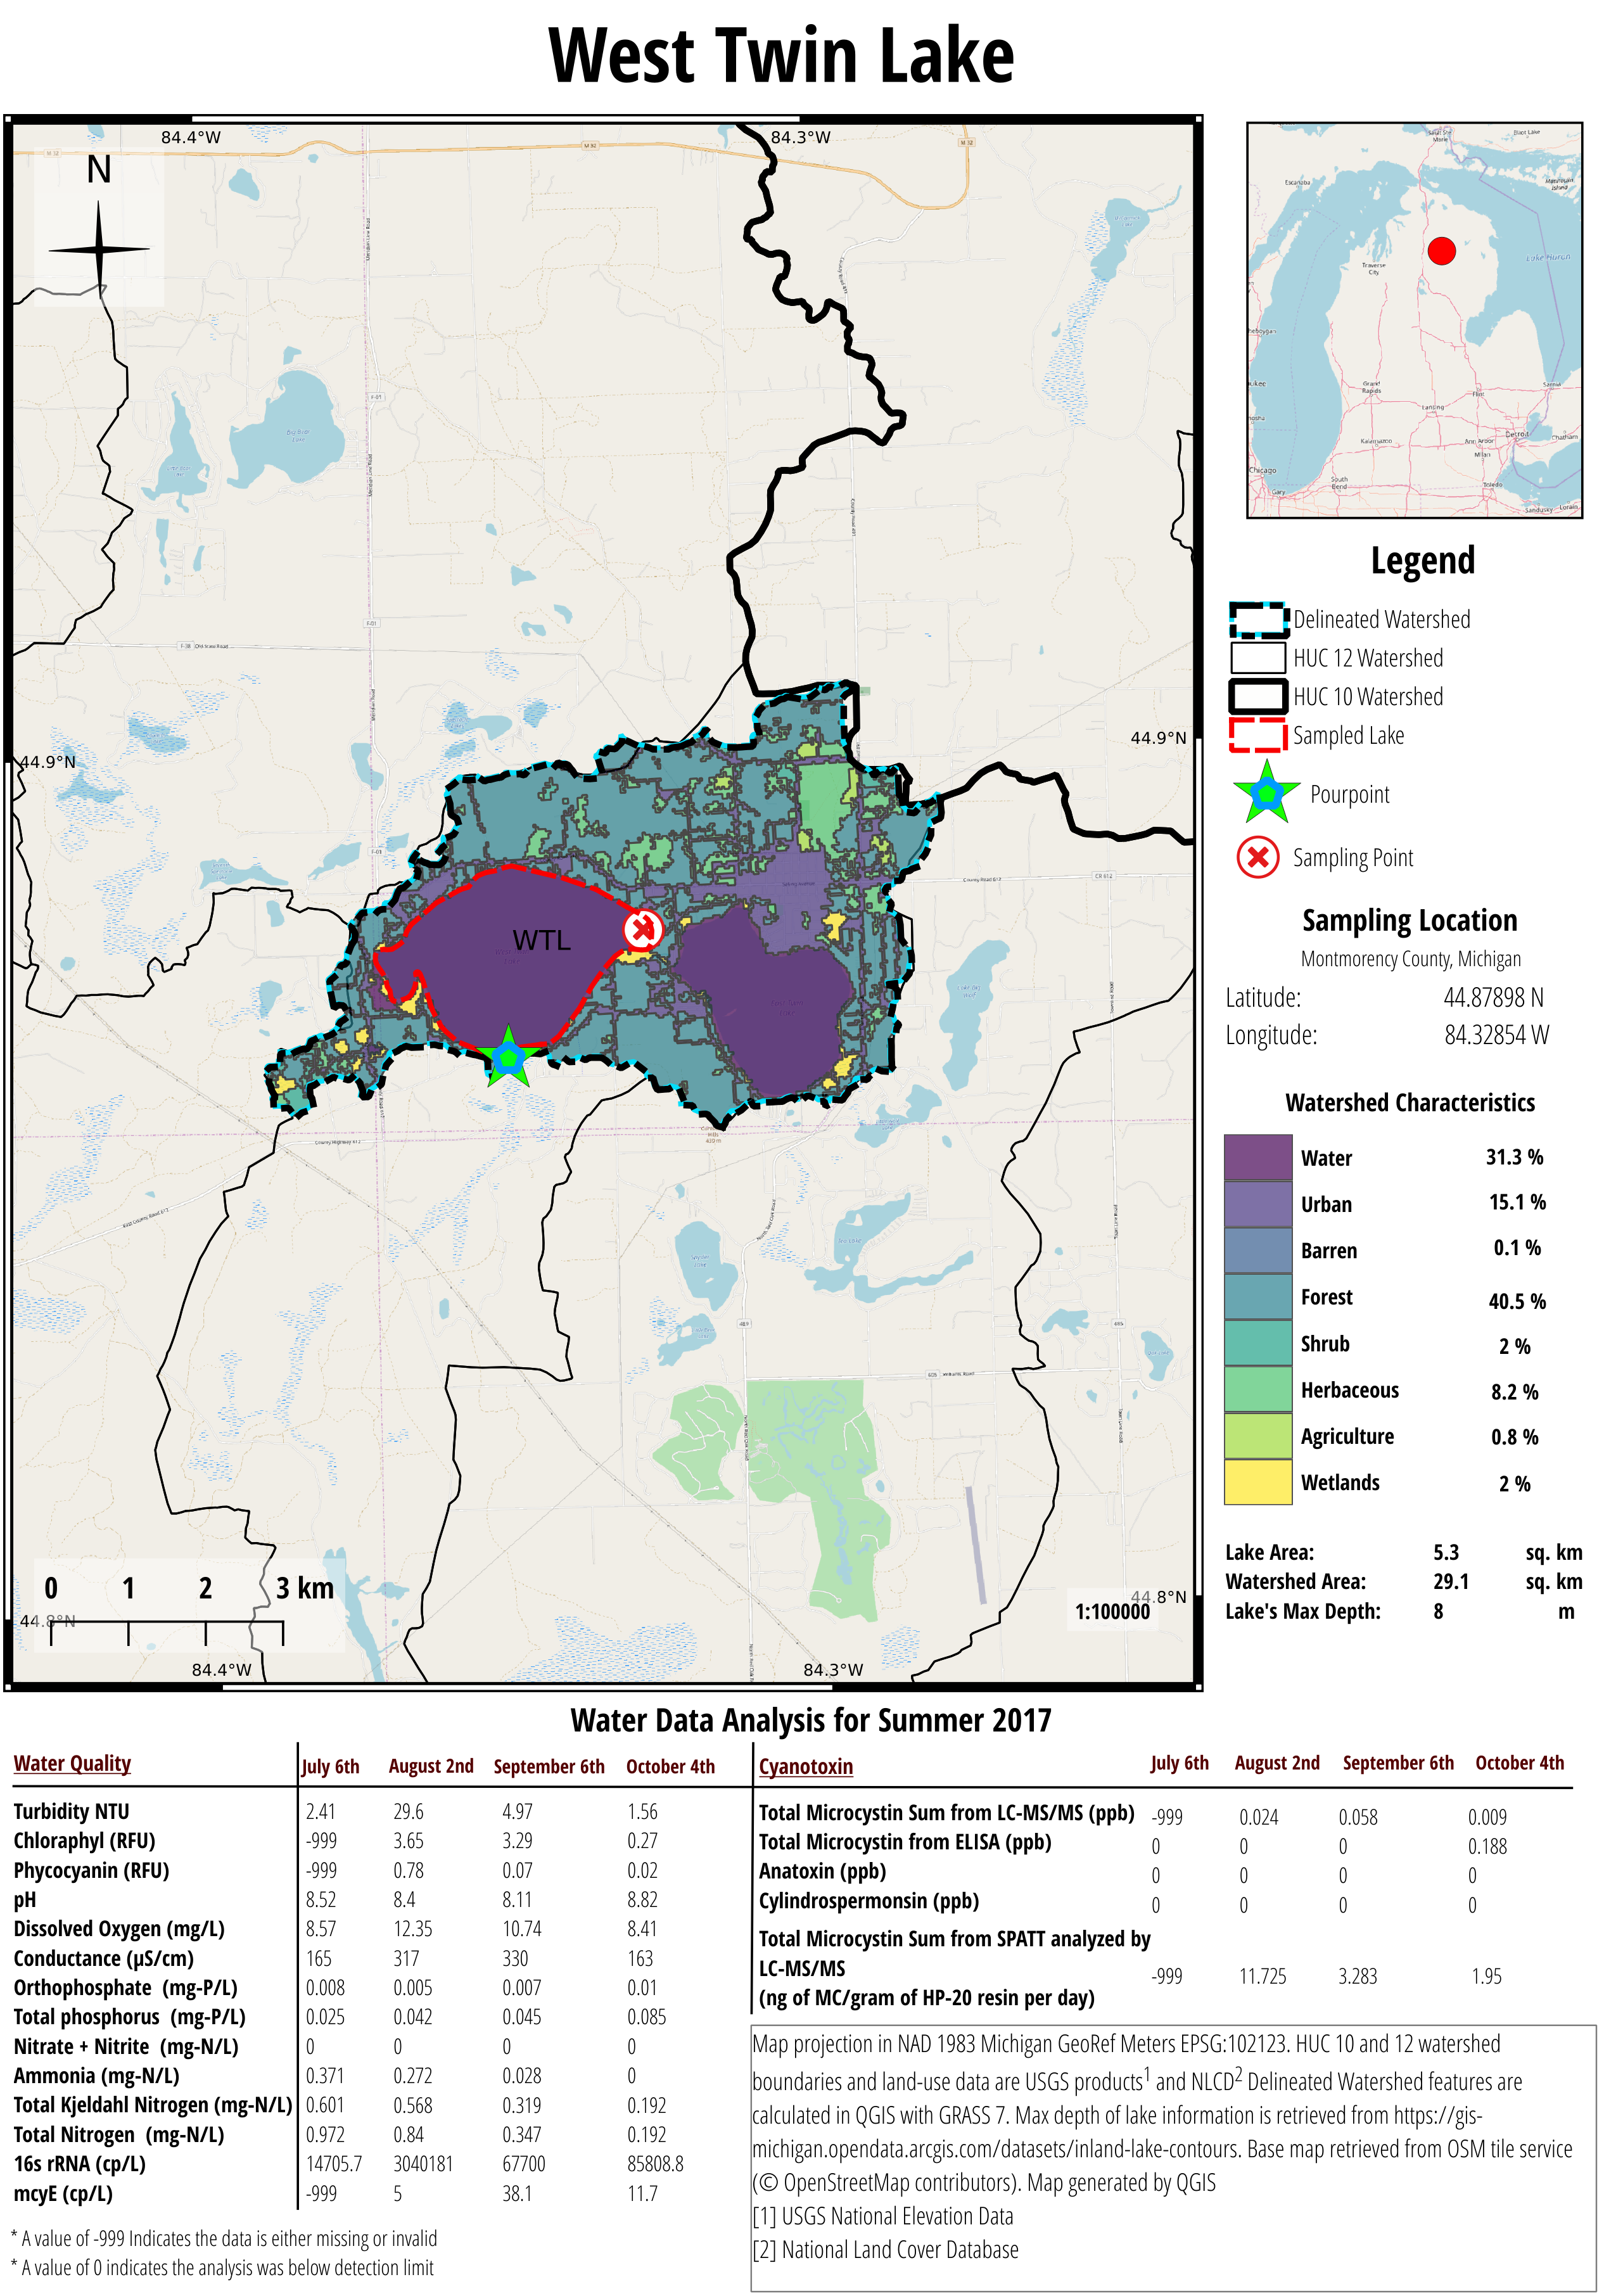
\includegraphics{figures/atlas/output_29}}
  }
\caption{GIS Map of West Twin Lake}
\end{figure}


\end{appendix}

\end{document}
